\documentclass{cmspaper}
\usepackage{graphicx}
\usepackage{amsmath}
\usepackage{amssymb}
\usepackage{subfigure}
\usepackage{multirow}
\usepackage{array}
\usepackage[pdfborder=0 0 0,
            colorlinks,
            urlcolor = blue,
            linkcolor = black,
            citecolor = black,
            menucolor = black,]
           {hyperref}
%% \usepackage[colorlinks]{hyperref}
%% \usepackage{url}
\usepackage[toc,page]{appendix}
\usepackage{varioref}
\renewcommand{\appendixname}{Appendix}
%% \renewcommand{\appendixtocname}{List of appendices}

%-------------------------------------------------------------------------------
% private environments
%-------------------------------------------------------------------------------

\newcommand{\customChapter}[1]{\chapter{\boldmath #1 \unboldmath}}
\newcommand{\customSection}[1]{\section{\boldmath #1 \unboldmath}}
\newcommand{\customSubsection}[1]{\boldmath\subsection{#1}\unboldmath}
\newcommand{\customSubsubsection}[1]{\boldmath\subsubsection{#1}\unboldmath}

%-------------------------------------------------------------------------------
% technical reference definitions
%-------------------------------------------------------------------------------

\newcommand{\AppendixRef}[1]{Appendix~\ref{#1}}
\newcommand{\EquationRef}[1]{Equation~(\ref{#1})}
\newcommand{\FigureRef}[1]{Figure~\ref{#1}}
\newcommand{\ReferenceRef}[1]{Reference~\cite{#1}}
\newcommand{\SectionRef}[1]{Section~\ref{#1}}
\newcommand{\TableRef}[1]{Table~\ref{#1}}

%-------------------------------------------------------------------------------
% unit definitions
%-------------------------------------------------------------------------------

\newcommand{\fs}{\ensuremath{\mathrm{fs}}}
\newcommand{\ps}{\ensuremath{\mathrm{ps}}}
\newcommand{\ns}{\ensuremath{\mathrm{ns}}}
\newcommand{\ips}{\ensuremath{\mathrm{ps^{-1}}}}
\newcommand{\um}{\ensuremath{\mathrm{\mu m}}}
\newcommand{\mm}{\ensuremath{\mathrm{mm}}}
\newcommand{\cm}{\ensuremath{\mathrm{cm}}}
\renewcommand{\deg}{\ensuremath{^\mathrm{o}}}
\newcommand{\ifb}{\ensuremath{\mathrm{fb^{-1}}}}
\newcommand{\ipb}{\ensuremath{\mathrm{pb^{-1}}}}
\newcommand{\inb}{\ensuremath{\mathrm{nb^{-1}}}}
\newcommand{\iub}{\ensuremath{\mathrm{\mu b^{-1}}}}
\newcommand{\fb}{\ensuremath{\mathrm{fb}}}
\newcommand{\pb}{\ensuremath{\mathrm{pb}}}
\newcommand{\nb}{\ensuremath{\mathrm{nb}}}
\newcommand{\ub}{\ensuremath{\mathrm{\mu b}}}
\newcommand{\eV}{\ensuremath{\mathrm{e\kern -0.1em V}}}
\newcommand{\keV}{\ensuremath{\mathrm{ke\kern -0.1em V}}}
\newcommand{\MeV}{\ensuremath{\mathrm{Me\kern -0.1em V}}}
\newcommand{\GeV}{\ensuremath{\mathrm{Ge\kern -0.1em V}}}
\newcommand{\TeV}{\ensuremath{\mathrm{Te\kern -0.1em V}}}
\newcommand{\eVc}{\ensuremath{\mathrm{e\kern -0.1em V/}c}}
\newcommand{\keVc}{\ensuremath{\mathrm{ke\kern -0.1em V/}c}}
\newcommand{\MeVc}{\ensuremath{\mathrm{Me\kern -0.1em V/}c}}
\newcommand{\GeVc}{\ensuremath{\mathrm{Ge\kern -0.1em V/}c}}
\newcommand{\TeVc}{\ensuremath{\mathrm{Te\kern -0.1em V/}c}}
\newcommand{\eVcc}{\ensuremath{\mathrm{e\kern -0.1em V/}c^2}}
\newcommand{\keVcc}{\ensuremath{\mathrm{ke\kern -0.1em V/}c^2}}
\newcommand{\MeVcc}{\ensuremath{\mathrm{Me\kern -0.1em V/}c^2}}
\newcommand{\GeVcc}{\ensuremath{\mathrm{Ge\kern -0.1em V/}c^2}}
\newcommand{\TeVcc}{\ensuremath{\mathrm{Te\kern -0.1em V/}c^2}}
\newcommand{\Tesla}{\ensuremath{\mathrm{T}}}

\newcommand{\kB}{\ensuremath{\mathrm{kBytes}}}
\newcommand{\MB}{\ensuremath{\mathrm{MBytes}}}
\newcommand{\GB}{\ensuremath{\mathrm{GBytes}}}
\newcommand{\PB}{\ensuremath{\mathrm{PBytes}}}
\newcommand{\TB}{\ensuremath{\mathrm{TBytes}}}
\newcommand{\kBs}{\ensuremath{\mathrm{kBytes/s}}}
\newcommand{\MBs}{\ensuremath{\mathrm{MBytes/s}}}

\newcommand{\Hz}{\ensuremath{\mathrm{Hz}}}
\newcommand{\kHz}{\ensuremath{\mathrm{kHz}}}
\newcommand{\MHz}{\ensuremath{\mathrm{MHz}}}
\newcommand{\GHz}{\ensuremath{\mathrm{GHz}}}

\newcommand{\icmSQs}{\ensuremath{\mathrm{cm^{-2}s^{-1}}}}

%-------------------------------------------------------------------------------
% reconstruction variable definitions
%-------------------------------------------------------------------------------

\newcommand{\SQS}{\ensuremath{\sqrt{s}}}
\newcommand{\ILUM}{\ensuremath{{\cal L}}}
\newcommand{\TZ}{\ensuremath{t_0}}
\newcommand{\PHISIX}{\ensuremath{\mathrm{\phi_6}}}
\newcommand{\PHIZERO}{\ensuremath{\mathrm{\phi_0}}}
\newcommand{\DPHI}{\ensuremath{\mathrm{\Delta \phi}}}
\newcommand{\ETA}{\ensuremath{\mathrm{\eta}}}
\newcommand{\DZERO}{\ensuremath{\mathrm{d_0}}}
\newcommand{\DZEB}{\ensuremath{\mathrm{d_B}}}
\newcommand{\PT}{\ensuremath{p_{T}}}
\newcommand{\Y}{\ensuremath{\mathrm{y}}}
\newcommand{\BDCUTS}{\ensuremath{\mathrm{\PT(\BD)>6\,\GeV;~|\Y| < 1}}}
\newcommand{\XSBD}{\ensuremath{\mathrm{\sigma_\BD}}}
\newcommand{\XSTOT}{\ensuremath{\mathrm{\sigma_{total}}}}

\newcommand{\Br}{\ensuremath{{\cal B}}}

%-------------------------------------------------------------------------------
% CKM matrix related
%-------------------------------------------------------------------------------

\newcommand{\LAM}{\ensuremath{\mathrm{\lambda}}}
\newcommand{\RHO}{\ensuremath{\mathrm{\rho}}}
%\newcommand{\ETA}{\ensuremath{\mathrm{\eta}}}

\newcommand{\VCKM}{\ensuremath{\mathrm{V}}}
\newcommand{\VCKMd}{\ensuremath{\mathrm{V^\dagger}}}

\newcommand{\VUD}{\ensuremath{\mathrm{V_{ud}}}}
\newcommand{\VUS}{\ensuremath{\mathrm{V_{us}}}}
\newcommand{\VUB}{\ensuremath{\mathrm{V_{ub}}}}
\newcommand{\VCD}{\ensuremath{\mathrm{V_{cd}}}}
\newcommand{\VCB}{\ensuremath{\mathrm{V_{cb}}}}
\newcommand{\VCS}{\ensuremath{\mathrm{V_{cs}}}}
\newcommand{\VTB}{\ensuremath{\mathrm{V_{tb}}}}
\newcommand{\VTD}{\ensuremath{\mathrm{V_{td}}}}
\newcommand{\VTS}{\ensuremath{\mathrm{V_{ts}}}}

\newcommand{\VUDs}{\ensuremath{\mathrm{V^*_{ud}}}}
\newcommand{\VUBs}{\ensuremath{\mathrm{V^*_{ub}}}}
\newcommand{\VCDs}{\ensuremath{\mathrm{V^*_{cd}}}}
\newcommand{\VCBs}{\ensuremath{\mathrm{V^*_{cb}}}}
\newcommand{\VCSs}{\ensuremath{\mathrm{V^*_{cs}}}}
\newcommand{\VTBs}{\ensuremath{\mathrm{V^*_{tb}}}}
\newcommand{\VTDs}{\ensuremath{\mathrm{V^*_{td}}}}
\newcommand{\VTSs}{\ensuremath{\mathrm{V^*_{ts}}}}

%-------------------------------------------------------------------------------
% physics parameter definitions
%-------------------------------------------------------------------------------

\newcommand{\EPS}{\ensuremath{\varepsilon}}
\newcommand{\DIL}{\ensuremath{\rm D}}
\newcommand{\EPSDSQ}{\ensuremath{\rm \varepsilon D^2}}

\newcommand{\SINTA}{\ensuremath{\sin 2 \alpha}}
\newcommand{\SINTB}{\ensuremath{\sin 2 \beta}}

\newcommand{\PHIDNP}{\ensuremath{\mathrm{\phi^d_{NP}}}}
\newcommand{\PHISNP}{\ensuremath{\mathrm{\phi^s_{NP}}}}

\newcommand{\FU}{\ensuremath{\mathrm{f_u}}}
\newcommand{\FD}{\ensuremath{\mathrm{f_d}}}
\newcommand{\FS}{\ensuremath{\mathrm{f_s}}}
\newcommand{\FLB}{\ensuremath{\mathrm{f_{\Lambda_B}}}}
\newcommand{\EPSB}{\ensuremath{\varepsilon_\mathrm{b}}}

\newcommand{\GBS}{\ensuremath{\Gamma_s}}
\newcommand{\DGBS}{\ensuremath{\Delta \Gamma_s}}
\newcommand{\MBS}{\ensuremath{m_\BS}}
\newcommand{\DMS}{\ensuremath{\Delta m_s}}
\newcommand{\XS}{\ensuremath{x_s}}

\newcommand{\GBD}{\ensuremath{\Gamma_\mathrm{d}}}
\newcommand{\DGBD}{\ensuremath{\Delta \Gamma_\mathrm{d}}}
\newcommand{\DG}{\ensuremath{\Delta\Gamma}}
\newcommand{\DGG}{\ensuremath{\Delta\Gamma/\Gamma}}
\newcommand{\DGGS}{\ensuremath{\Delta\Gamma_s/\Gamma_s}}
\newcommand{\MBD}{\ensuremath{m_d}}
\newcommand{\DMD}{\ensuremath{\Delta m_d}}
\newcommand{\XD}{\ensuremath{x_d}}

\newcommand{\MT}{\ensuremath{m_t}}

%-------------------------------------------------------------------------------
% particle definitions
%-------------------------------------------------------------------------------

% single particles - bosons
\newcommand{\GAM}{\ensuremath{\gamma}}
\newcommand{\Z}{\ensuremath{Z}}
\newcommand{\W}{\ensuremath{W}}
\newcommand{\WP}{\ensuremath{W^+}}
\newcommand{\WM}{\ensuremath{W^-}}
\newcommand{\WPM}{\ensuremath{W^\pm}}
\newcommand{\WMP}{\ensuremath{W^\mp}}
\newcommand{\Higgs}{\ensuremath{H}}

% single particles - leptons
\newcommand{\EL}{\ensuremath{e}}
\newcommand{\ELP}{\ensuremath{e^+}}
\newcommand{\ELM}{\ensuremath{e^-}}
\newcommand{\MU}{\ensuremath{\mu}}
\newcommand{\MUP}{\ensuremath{\mu^+}}
\newcommand{\MUM}{\ensuremath{\mu^-}}
\newcommand{\TAU}{\ensuremath{\tau}}
\newcommand{\TAUP}{\ensuremath{\tau^+}}
\newcommand{\TAUM}{\ensuremath{\tau^-}}
\newcommand{\LP}{\ensuremath{\ell^{+}}}
\newcommand{\LM}{\ensuremath{\ell^{-}}}
\newcommand{\NL}{\ensuremath{\nu_{\ell}}}
\newcommand{\NLB}{\ensuremath{\overline{\nu}_{\ell}}}

% single particles - quarks
\newcommand{\up}{\ensuremath{u}}
\newcommand{\down}{\ensuremath{d}}
\newcommand{\strange}{\ensuremath{s}}
\newcommand{\charm}{\ensuremath{c}}
\newcommand{\bottom}{\ensuremath{b}}
\newcommand{\topquark}{\ensuremath{t}}
\newcommand{\ubar}{\ensuremath{\bar{u}}}
\newcommand{\dbar}{\ensuremath{\bar{d}}}
\newcommand{\sbar}{\ensuremath{\bar{s}}}
\newcommand{\cbar}{\ensuremath{\bar{c}}}
\newcommand{\bbar}{\ensuremath{\bar{b}}}
\newcommand{\tbar}{\ensuremath{\bar{t}}}




% single particles - B hadrons
\newcommand{\B}{\ensuremath{B}}
\newcommand{\BU}{\ensuremath{\mathrm{B_u}}}
\newcommand{\BUP}{\ensuremath{\mathrm{B^+}}}
\newcommand{\BUM}{\ensuremath{\mathrm{B^-}}}
\newcommand{\BD}{\ensuremath{\mathrm{B^0}}}
\newcommand{\BDB}{\ensuremath{\mathrm{\overline{B^0}}}}
\newcommand{\BS}{\ensuremath{\mathrm{B_s}}}
\newcommand{\BSB}{\ensuremath{\mathrm{\overline{B}_s}}}
\newcommand{\BC}{\ensuremath{\mathrm{B_c}}}
\newcommand{\BCP}{\ensuremath{\mathrm{B_c^+}}}
\newcommand{\BCM}{\ensuremath{\mathrm{B_c^-}}}
\newcommand{\LB}{\ensuremath{\mathrm{\Lambda_b}}}
\newcommand{\LBB}{\ensuremath{\mathrm{\overline{\Lambda}_b}}}

% single particles - charmed hadrons
\newcommand{\D}{\ensuremath{D}}
\newcommand{\DZ}{\ensuremath{\mathrm{D^0}}}
\newcommand{\DZB}{\ensuremath{\mathrm{\overline{D}^0}}}
\newcommand{\DP}{\ensuremath{\mathrm{D^+}}}
\newcommand{\DM}{\ensuremath{\mathrm{D^-}}}
\newcommand{\DS}{\ensuremath{\mathrm{D_s}}}
\newcommand{\DSP}{\ensuremath{\mathrm{D^+_s}}}
\newcommand{\DSM}{\ensuremath{\mathrm{D^-_s}}}
\newcommand{\DSPM}{\ensuremath{\mathrm{D^\pm_s}}}
\newcommand{\DSMP}{\ensuremath{\mathrm{D^\mp_s}}}
\newcommand{\DSS}{\ensuremath{\mathrm{D^*_s}}}
\newcommand{\DSSP}{\ensuremath{\mathrm{D^{*\,+}_s}}}
\newcommand{\DSSM}{\ensuremath{\mathrm{D^{*\,-}_s}}}
\newcommand{\DSSPM}{\ensuremath{\mathrm{D^{*\,\pm}_s}}}
\newcommand{\DSSMP}{\ensuremath{\mathrm{D^{*\,\mp}_s}}}
\newcommand{\LC}{\ensuremath{\mathrm{\Lambda_c}}}
\newcommand{\LCP}{\ensuremath{\mathrm{\Lambda_c^+}}}
\newcommand{\LCM}{\ensuremath{\mathrm{\Lambda_c^-}}}
\newcommand{\SCZ}{\ensuremath{\mathrm{\Sigma_c^0}}}
\newcommand{\SCP}{\ensuremath{\mathrm{\Sigma_c^+}}}
\newcommand{\SCPP}{\ensuremath{\mathrm{\Sigma_c^{++}}}}

% single particles - quarkonia
\newcommand{\UPSI}{\ensuremath{\Upsilon}}
\newcommand{\JPSI}{\ensuremath{\mathrm{J/\psi}}}
\newcommand{\PHI}{\ensuremath{\phi}}

% single particles - kaons
\newcommand{\K}{\ensuremath{K}}
\newcommand{\KP}{\ensuremath{\mathrm{K^+}}}
\newcommand{\KM}{\ensuremath{\mathrm{K^-}}}
\newcommand{\KPM}{\ensuremath{\mathrm{K^\pm}}}
\newcommand{\KMP}{\ensuremath{\mathrm{K^\mp}}}
\newcommand{\KZ}{\ensuremath{\mathrm{K^0}}}
\newcommand{\KZB}{\ensuremath{\mathrm{\overline{K}^0}}}
\newcommand{\KS}{\ensuremath{\mathrm{K^*}}}
\newcommand{\KSZ}{\ensuremath{\mathrm{K^{*\,0}}}}
\newcommand{\KZS}{\ensuremath{\mathrm{K^0_S}}}
\newcommand{\KZL}{\ensuremath{\mathrm{K^0_L}}}
\newcommand{\LS}{\ensuremath{\mathrm{\Lambda}}}
\newcommand{\SSZ}{\ensuremath{\mathrm{\Sigma^0}}}
\newcommand{\SSP}{\ensuremath{\mathrm{\Sigma^{+}}}}
\newcommand{\SSM}{\ensuremath{\mathrm{\Sigma^{-}}}}

% single particles - pions
\newcommand{\PI}{\ensuremath{\pi}}
\newcommand{\PIZ}{\ensuremath{\pi^0}}
\newcommand{\PIP}{\ensuremath{\pi^+}}
\newcommand{\PIM}{\ensuremath{\pi^-}}

% single particles - protons
\newcommand{\PR}{\ensuremath{p}}
\newcommand{\PRB}{\ensuremath{\overline{p}}}

% particle pairs
\newcommand{\EE}{\ensuremath{e^+e^-}}
\newcommand{\PPBAR}{\ensuremath{p\overline{p}}}
\newcommand{\BBBAR}{\ensuremath{b\overline{b}}}
\newcommand{\CCBAR}{\ensuremath{c\overline{c}}}
\newcommand{\ZZ}{\ensuremath{ZZ}}
\newcommand{\WW}   {\ensuremath{\WP\WM}}
\newcommand{\TTBAR}{\ensuremath{t \bar{t}}}

% more complicated particle combination
\newcommand{\WPlusJets}{\ensuremath{W\mathrm{+Jets}}}
\newcommand{\WPlusGamma}{\ensuremath{W\mathrm{+}\gamma}}
\newcommand{\Wb}{\ensuremath{Wb}}
\newcommand{\Wc}{\ensuremath{Wc}}
\newcommand{\Wbb}{\ensuremath{Wbb}}
\newcommand{\Wcc}{\ensuremath{Wcc}}

%-------------------------------------------------------------------------------
% particle decay chain definitions
%-------------------------------------------------------------------------------

% helper
\renewcommand{\to}{\ensuremath{\rightarrow}}

% Higgs decays
\newcommand{\HiggsToWW}   {\ensuremath{\Higgs \to \WP\WM}}
\newcommand{\HiggsToZZ}   {\ensuremath{\Higgs \to \ZZ}}
\newcommand{\ZToTauTau}   {\ensuremath{\Z \to \TAUP\TAUM}}
\newcommand{\ZToEE}       {\ensuremath{\Z \to \Ep\Em}}
\newcommand{\ZToMuMu}     {\ensuremath{\Z \to \Mup\Mum}}
\newcommand{\ZToEEGamma}       {\ensuremath{\Z \to \Ep\Em\gamma}}
\newcommand{\ZToLL}       {\ensuremath{\Z \to \LP\LM}}
\newcommand{\HiggsToGammaGamma} {\ensuremath{\Higgs \to \gamma\gamma}}


% Lambda_b hadronic decays
\newcommand{\LBPRDZPI}   {\ensuremath{\LB \to \PR \DZ \PIP}}
\newcommand{\LBLCDS}     {\ensuremath{\LB \to \LCP \DSM}}
\newcommand{\LBLCDSS}    {\ensuremath{\LB \to \LCP \DSSM}}
\newcommand{\LBLCDSPIPI} {\ensuremath{\LB \to \LCP \DSM \PIP \PIM}}
\newcommand{\LBLCDSSPIPI}{\ensuremath{\LB \to \LCP \DSSM \PIP \PIM}}
\newcommand{\LBPRDS}     {\ensuremath{\LB \to \PR \DSM}}
\newcommand{\LBPRDSS}    {\ensuremath{\LB \to \PR \DSSM}}
\newcommand{\LBPRDSPIPI} {\ensuremath{\LB \to \PR \DSM \PIP \PIM}}
\newcommand{\LBPRDSSPIPI}{\ensuremath{\LB \to \PR \DSSM \PIP \PIM}}
\newcommand{\LBLCPI}     {\ensuremath{\LB \to \LCP \PIM}}
\newcommand{\LBLCPIPIPI} {\ensuremath{\LB \to \LCP \PIM \PIP \PIM}}
\newcommand{\LBSCZPIPI}  {\ensuremath{\LB \to \SCZ \PIM \PIP}}
\newcommand{\LBSCPPPIPI} {\ensuremath{\LB \to \SCPP \PIM \PIM}}
\newcommand{\LBPRPI}     {\ensuremath{\LB \to \PR \PIM}}
\newcommand{\LBPRPIPIPI} {\ensuremath{\LB \to \PR \PIM \PIP \PIM}}
\newcommand{\LBPRK}      {\ensuremath{\LB \to \PR \KM}}

% Lambda_c hadronic decays
\newcommand{\LCPRKPI}   {\ensuremath{\LCP \to \PR \KM \PIP}}
\newcommand{\LCLSPIPIPI}{\ensuremath{\LCP \to \LS \PIP \PIM \PIP}}
\newcommand{\LCLSPI}    {\ensuremath{\LCP \to \LS \PIP}}

% Sigma_c hadronic decays
\newcommand{\SCZLCPI}   {\ensuremath{\SCZ \to \LCP \PIM}}
\newcommand{\SCPPLCPI}  {\ensuremath{\SCPP \to \LCP \PIP}}

% Bs hadronic decays
\newcommand{\BSDSPI}   {\ensuremath{\BS \to \DSM \PIP}}
\newcommand{\BSDSSPI}  {\ensuremath{\BS \to \DSSM \PIP}}
\newcommand{\BSDSTPI}  {\ensuremath{\BS \to \DSM \PIP \PIP \PIM}}
\newcommand{\BSDSSTPI} {\ensuremath{\BS \to \DSSM \PIP \PIP \PIM}}
\newcommand{\BSDSDS}   {\ensuremath{\BS \to \DSM \DSP}}
\newcommand{\BSDSSDS}  {\ensuremath{\BS \to \DSSPM \DSMP}}
\newcommand{\BSDSSDSS} {\ensuremath{\BS \to \DSSM \DSSP}}
\newcommand{\BSDSKPHI} {\ensuremath{\BS \to \DSPM \KMP \PHI }}
\newcommand{\BSDSSKPHI}{\ensuremath{\BS \to \DSSPM \KMP \PHI }}
\newcommand{\BSKK}     {\ensuremath{\BS \to \KM \KP}}
\newcommand{\BSKPI}    {\ensuremath{\BS \to \KM \PIP}}

% Bs leptonic decays
\newcommand{\BSJPSIPHI}{\ensuremath{\BS \to \JPSI \PHI}}
\newcommand{\BSNLDSX}  {\ensuremath{\BS \to \NL \LP \DSM X}}

% Bd hadronic decays
\newcommand{\BDPIPI}   {\ensuremath{\BD \to \PIM \PIP}}
\newcommand{\BDPIK}    {\ensuremath{\BD \to \PIM \KP}}
\newcommand{\BDJPSIKS} {\ensuremath{\BD \to \JPSI \KZS}}

% Ds* decays
\newcommand{\DSSDSGP}  {\ensuremath{\DSS \to \DS \gamma,\PIZ}}

% Ds decays
\newcommand{\DSPHIPI}  {\ensuremath{\DSM \to \PHI \PIM}}
\newcommand{\DSKSK}    {\ensuremath{\DSM \to \KSZ \KM}}
\newcommand{\DSPIPIPI} {\ensuremath{\DSM \to \PIM \PIP \PIM}}
\newcommand{\DSKZSK}   {\ensuremath{\DSM \to \KZS \KM}}
\newcommand{\DSTPI}    {\ensuremath{\DSM \to \PIM \PIM \PIP}}
\newcommand{\DSKKZSPIPI}{\ensuremath{\DSM \to \KP \KZS \PIM \PIM}}
\newcommand{\DSPHITPI} {\ensuremath{\DSM \to \PHI \PIM \PIM \PIP}}
\newcommand{\DSKPIPI}  {\ensuremath{\DSM \to \KM \PIM \PIP}}
\newcommand{\DSNLLPHIX}{\ensuremath{\DSM \to \NLB \LP \PHI   X}}
\newcommand{\DSALL}    {\ensuremath{\DSM \to \rm all \,\, above }}

% D decays
\newcommand{\DZKPI}    {\ensuremath{\DZ \to \KM \PIP}}
\newcommand{\DZKPIPIPI}{\ensuremath{\DZ \to \KM \PIP \PIM \PIP}}

% Lambda_c hadronic decays
\newcommand{\LSPRPI}   {\ensuremath{\LS \to \PR \PIM}}

% Phi decays
\newcommand{\PHIKK}    {\ensuremath{\PHI \to \KM \KP}}

% K* decays
\newcommand{\KSKPI}    {\ensuremath{\KSZ \to \KP \PIM}}

% Kshort decays
\newcommand{\KZSPIPI}  {\ensuremath{\KZS \to \KP \PIM}}


\newcommand{\CLs}{\ensuremath{CL_\mathrm{s}}}
\newcommand{\CLb}{\ensuremath{CL_\mathrm{b}}}
\newcommand{\CLsb}{\ensuremath{CL_\mathrm{s+b}}}

\newcommand{\grad}{\ensuremath{^{\circ}}}
%
% Special user made math symbols
%
\newcommand{\lsim}{\raisebox{-1.5mm}{$\:\stackrel{\textstyle{<}}{\textstyle{\sim}}\:$}}
\newcommand{\gsim}{\raisebox{-1.5mm}{$\:\stackrel{\textstyle{>}}{\textstyle{\sim}}\:$}}

% particles

\newcommand{\pipm}{\ensuremath{\pi^{\pm}}}
\newcommand{\pizero}{\ensuremath{\pi^{0}}}
\newcommand{\Kpm}{\ensuremath{K^{\pm}}}
\newcommand{\Hi}{\ensuremath{H}}
\newcommand{\Wjets}{\ensuremath{W+\mathrm{jets}}}
\newcommand{\Zjets}{\ensuremath{Z+\mathrm{jets}}}
\newcommand{\Wt}{\ensuremath{\mathrm{Wt}}}
\newcommand{\Wstar}{\ensuremath{W^{*}}}
\newcommand{\Wparenthesisstar}{\ensuremath{W^{(*)}}}
\newcommand{\Zstar}{\ensuremath{Z^{*}}}
\newcommand{\WZ}{\ensuremath{\W\Z}}
\newcommand{\E}{\ensuremath{\mathrm{e}}}
\newcommand{\Ep}{\ensuremath{\mathrm{e}^{+}}}
\newcommand{\Em}{\ensuremath{\mathrm{e}^{-}}}
\newcommand{\Epm}{\ensuremath{\mathrm{e}^{\pm}}}
\newcommand{\Emp}{\ensuremath{\mathrm{e}^{\mp}}}
\newcommand{\Mu}{\ensuremath{\mu}}
\newcommand{\Mup}{\ensuremath{\mu^{+}}}
\newcommand{\Mum}{\ensuremath{\mu^{-}}}
\newcommand{\Mupm}{\ensuremath{\mu^{\pm}}}
\newcommand{\Mump}{\ensuremath{\mu^{\mp}}}
\newcommand{\Tau}{\ensuremath{\tau}}
\newcommand{\Taup}{\ensuremath{\tau^{+}}}
\newcommand{\Taum}{\ensuremath{\tau^{-}}}
\newcommand{\Taupm}{\ensuremath{\tau^{\pm}}}
\newcommand{\Taump}{\ensuremath{\tau^{\mp}}}
\newcommand{\Nu}{\ensuremath{\nu}}
\newcommand{\Nubar}{\ensuremath{\bar{\nu}}}
\newcommand{\Lep}{\ensuremath{\ell}}
\newcommand{\Lepp}{\ensuremath{\ell^{+}}}
\newcommand{\Lepm}{\ensuremath{\ell^{-}}}
\newcommand{\Lprime}{\ensuremath{\Lep^{\prime}}}
\newcommand{\Prot}{\ensuremath{p}}
\newcommand{\Pbar}{\ensuremath{\bar{p}}}
\newcommand{\PP}{\Prot\Prot}
\newcommand{\PPbar}{\Prot\Pbar}
\newcommand{\ttbar}{\ensuremath{t\bar{t}}}
\newcommand{\qq}{\ensuremath{\mathrm{q}\mathrm{q}}}
\newcommand{\bbbar}{\ensuremath{\mathrm{b}\bar{\mathrm{b}}}}
\newcommand{\Wtb}{\ensuremath{\W\mathrm{t}\mathrm{b}}}
\newcommand{\Top}{\ensuremath{\mathrm{t}}}
\newcommand{\Bot}{\ensuremath{\mathrm{b}}}
\newcommand{\Atop}{\ensuremath{\bar{\mathrm{t}}}}
\newcommand{\Abot}{\ensuremath{\bar{\mathrm{b}}}}
% arrow
\newcommand{\To}{\ensuremath{\rightarrow}}

% masses
\newcommand{\mHi}{\ensuremath{m_{\mathrm{Higgs}}}}
\newcommand{\mW}{\ensuremath{m_{\mathrm{W}}}}
\newcommand{\mZ}{\ensuremath{m_{\mathrm{Z}}}}
\newcommand{\mll}{\ensuremath{m_{\Lep\Lep}}}


% kinematics
\newcommand{\pt}{\ensuremath{p_\mathrm{T}}}
\newcommand{\ptHat}{\ensuremath{\hat{p_\mathrm{T}}}}
\newcommand{\ptveto}{\ensuremath{\pt^\mathrm{veto}}}
\newcommand{\ptl}{\ensuremath{p_\perp^{\Lep}}}
\newcommand{\ptlmax}{\ensuremath{p_{\mathrm{T}}^{\Lep,\mathrm{max}}}}
\newcommand{\ptlmin}{\ensuremath{p_{\mathrm{T}}^{\Lep,\mathrm{min}}}}
\newcommand{\met}{\ensuremath{\Et^{\mathrm{miss}}}}
\newcommand{\delphill}{\ensuremath{\Delta\phi_{\Lep\Lep}}}
\newcommand{\deletall}{\ensuremath{\Delta\eta_{\Lep\Lep}}}
\newcommand{\delphimetl}{\ensuremath{\Delta\phi_{\met\Lep}}}
\newcommand{\deltaRll}{\ensuremath{\Delta\mathrm{R}_{\Lep\Lep}}}
\newcommand{\delphimetdilep}{\ensuremath{\Delta\phi_{\met,\Lep\Lep}}}
\newcommand{\delphimetLeadingJet}{\ensuremath{\Delta\phi_{\met,\mathrm{leading\ jet}}}}
\newcommand{\Et}{\ensuremath{E_\mathrm{T}}}
\newcommand{\delR}{\ensuremath{\Delta R}}
\newcommand{\Eta}{\ensuremath{\eta}}
\newcommand{\mT}{\ensuremath{m_{T}^{\ell\ell \met}}}


%efficiencies
\newcommand{\effsig}{\ensuremath{\varepsilon_{\mathrm{bkg}}^{\mathrm{S}}}}
\newcommand{\effnorm}{\ensuremath{\varepsilon_{\mathrm{bkg}}^{\mathrm{N}}}}
\newcommand{\Nsig}{\ensuremath{N_{\mathrm{bkg}}^{\mathrm{S}}}}
\newcommand{\Nnorm}{\ensuremath{N_{\mathrm{bkg}}^{\mathrm{N}}}}
\newcommand{\epsilonFake}{\ensuremath{\varepsilon_{\mathrm{fake}}}}

% processes
\newcommand{\dyee}{\ensuremath{Z/\gamma^*\to ee}}
\newcommand{\dymm}{\ensuremath{Z/\gamma^*\to\mu\mu}}
\newcommand{\dytt}{\ensuremath{Z/\gamma^*\to\tau\tau}}
\newcommand{\dyll}{\ensuremath{Z/\gamma^*\to\ell\ell}}
\newcommand{\dy}{\ensuremath{Z/\gamma^*}}
\newcommand{\zee}{\ensuremath{Z\to ee}}
\newcommand{\zmm}{\ensuremath{Z\to\mu\mu}}
\newcommand{\ztt}{\ensuremath{Z\to\tau\tau}}
%\newcommand{\ttbar}{\ensuremath{t\bar{t}}}
\newcommand{\ppww}{\ensuremath{pp \to W^+W^-}}
\newcommand{\wwll}{\ensuremath{WW\to \ell^+\ell^-}}
\newcommand{\wwlnln}{\ensuremath{W^+W^-\to \ell^+\nu \ell^-\bar{\nu}}}
\newcommand{\ww}{\ensuremath{WW}}
\newcommand{\wwpm}{\ensuremath{W^+W^-}}
\newcommand{\hww}{\ensuremath{H\to W^+W^-}}
\newcommand{\wz}{\ensuremath{WZ}}
\newcommand{\zz}{\ensuremath{ZZ}}
\newcommand{\wgamma}{\ensuremath{W\gamma}}
\newcommand{\wjets}{\ensuremath{W+}jets} 
\newcommand{\tw}{\ensuremath{tW}} 
\newcommand{\singletopt}{\ensuremath{t} ($t$-chan)} 
\newcommand{\singletops}{\ensuremath{t} ($s$-chan)} 
\newcommand{\z}{\ensuremath{\mathrm{Z}}}
\newcommand{\routin}{\ensuremath{R_{out/in}}}

%other 
\def\fixme{({\bf FixMe})}
\newcommand{\ee}{\ensuremath{ee}}
\newcommand{\emu}{\ensuremath{e\mu}}
\def\mm{\ensuremath{\mu\mu}}

% integrated luminosity
\newcommand{\intlumi}{4.9~\ifb}


\setcounter{topnumber}{1}
\setcounter{bottomnumber}{1}
\setcounter{secnumdepth}{6}
%===================================================================================================
\begin{document}
\begin{titlepage}

  \analysisnote{2012/XXX}

  \date{\today}

  \title{Matrix Element Based Discriminants for Higgs Look-Alike Particles}

  \begin{Authlist}
%
Y. Chen, E. DiMarco, M. Spiropulu, J. Veverka, S. Xie.
\Instfoot{caltech}{California Institute of Technology, Pasadena, USA}
B. Mangano, G. Petrucciani, V. Sharma, A. Vartak.
\Instfoot{ucsd}{University of California, San Diego, La Jolla, USA}
%

\end{Authlist}


  \begin{abstract}
  Abstract
  \end{abstract} 

\end{titlepage}
\tableofcontents
%\listoftables
%\listoffigures
\newpage 

%===================================================================================================
\section{Introduction}
  \label{sec:intro}

This is introduction!

\section{Detector Response Model}
\label{sec:DetectorResponseModel}
Besides the effect of the acceptance on the distribution of the independant discriminating observables,
the effects of lepton selection efficiency and lepton momentum resolution also play a role. The lepton
selection efficiency typically decreases severely between $15$~\GeV and $5$~\GeV, resulting in 
significant sculpting of the distributions of the important observables. Furthermore, the 
non-perfect energy and momentum measurement for electrons and muons also induce sculpting effects.

Ideally to build the probability density function for the matrix element discriminant input observables,
we would pass all events through the full detector simulation to fully parameterize all possible
detector effects. Unfortunately, this procedure is far too slow to be able to produce anything useful. 
We, instead, adopt the strategy of parametrizing the efficiency and energy response in sufficiently
small bins of $p_{T}$ and $\eta$ allowing us to roughly reproduce the detector response using many
orders of magnitude less computing time.

\subsection{Efficiency Model}
\label{sec:EfficiencyModel}
The efficiency map is built using the full simulation Monte Carlo sample of the ZZ process. 
The pileup is reweighted to the distribution observed in data. The efficiencies for 
electron selection are summarized in Tables \ref{tab:ElectronEfficiencyMap1}, 
\ref{tab:ElectronEfficiencyMap2}, and \ref{tab:ElectronEfficiencyMap3}. The efficiencies
for muon selection are summaized in Tables \ref{tab:MuonEfficiencyMap1}, 
\ref{tab:MuonEfficiencyMap2}, and \ref{tab:MuonEfficiencyMap3}.

\begin{table}[!htbp]
\begin{center}
\begin{tabular}{|c|c|c|c|c|c|}
\hline
$p_{T}$/$\eta$ Bin        &  0.00 - 0.20        &  0.20 - 0.40        &  0.40 - 0.60        &  0.60 - 0.80        &  0.80 - 1.00        \\
\hline
5.0 - 6.0~\GeV        & 0.055        & 0.053        & 0.054        & 0.048        & 0.044        \\
6.0 - 7.0~\GeV        & 0.093        & 0.092        & 0.098        & 0.086        & 0.078        \\
7.0 - 8.0~\GeV        & 0.467        & 0.509        & 0.523        & 0.519        & 0.482        \\
8.0 - 9.0~\GeV        & 0.618        & 0.669        & 0.671        & 0.683        & 0.644        \\
9.0 - 10.0~\GeV        & 0.716        & 0.741        & 0.755        & 0.754        & 0.725        \\
10.0 - 12.0~\GeV        & 0.794        & 0.826        & 0.820        & 0.816        & 0.800        \\
12.0 - 14.0~\GeV        & 0.841        & 0.868        & 0.868        & 0.858        & 0.844        \\
14.0 - 16.0~\GeV        & 0.870        & 0.886        & 0.890        & 0.889        & 0.862        \\
16.0 - 18.0~\GeV        & 0.879        & 0.902        & 0.906        & 0.894        & 0.888        \\
18.0 - 20.0~\GeV        & 0.894        & 0.915        & 0.907        & 0.906        & 0.890        \\
20.0 - 25.0~\GeV        & 0.903        & 0.922        & 0.920        & 0.915        & 0.902        \\
25.0 - 30.0~\GeV        & 0.914        & 0.931        & 0.933        & 0.926        & 0.913        \\
30.0 - 35.0~\GeV        & 0.921        & 0.938        & 0.940        & 0.933        & 0.925        \\
35.0 - 40.0~\GeV        & 0.925        & 0.941        & 0.943        & 0.937        & 0.927        \\
40.0 - 50.0~\GeV        & 0.931        & 0.944        & 0.948        & 0.942        & 0.935        \\
50.0 - 7000        & 0.942        & 0.956        & 0.957        & 0.950        & 0.947        \\
\hline
\end{tabular}
\caption{Table of electron selection efficiencies in bins of $p_{T}$ and $|\eta|$,
for $|\eta| < 1.0$}
\label{tab:ElectronEfficiencyMap1}
\end{center}
\end{table}


\begin{table}[!htbp]
\begin{center}
\begin{tabular}{|c|c|c|c|c|c|}
\hline
$p_{T}$/$\eta$ Bin        &  1.00 - 1.20        &  1.20 - 1.44        &  1.44 - 1.57        &  1.57 - 1.80        &  1.80 - 2.00        \\
\hline
5.0 - 6.0~\GeV        & 0.045        & 0.047        & 0.053        & 0.061        & 0.066        \\
6.0 - 7.0~\GeV        & 0.076        & 0.082        & 0.085        & 0.114        & 0.150        \\
7.0 - 8.0~\GeV        & 0.422        & 0.366        & 0.199        & 0.299        & 0.347        \\
8.0 - 9.0~\GeV        & 0.598        & 0.534        & 0.287        & 0.448        & 0.467        \\
9.0 - 10.0~\GeV        & 0.685        & 0.632        & 0.362        & 0.529        & 0.553        \\
10.0 - 12.0~\GeV        & 0.759        & 0.704        & 0.435        & 0.608        & 0.640        \\
12.0 - 14.0~\GeV        & 0.813        & 0.765        & 0.481        & 0.691        & 0.703        \\
14.0 - 16.0~\GeV        & 0.840        & 0.796        & 0.532        & 0.732        & 0.756        \\
16.0 - 18.0~\GeV        & 0.858        & 0.820        & 0.551        & 0.767        & 0.777        \\
18.0 - 20.0~\GeV        & 0.870        & 0.833        & 0.566        & 0.787        & 0.802        \\
20.0 - 25.0~\GeV        & 0.885        & 0.852        & 0.576        & 0.813        & 0.825        \\
25.0 - 30.0~\GeV        & 0.898        & 0.870        & 0.594        & 0.831        & 0.836        \\
30.0 - 35.0~\GeV        & 0.909        & 0.881        & 0.597        & 0.846        & 0.851        \\
35.0 - 40.0~\GeV        & 0.912        & 0.888        & 0.606        & 0.855        & 0.859        \\
40.0 - 50.0~\GeV        & 0.921        & 0.900        & 0.618        & 0.876        & 0.872        \\
50.0 - 7000~\GeV        & 0.936        & 0.925        & 0.651        & 0.906        & 0.902        \\
\hline
\end{tabular}
\caption{Table of electron selection efficiencies in bins of $p_{T}$ and $|\eta|$,
for $|\eta|$ between $1.0$ and $2.0$}
\label{tab:ElectronEfficiencyMap2}
\end{center}
\end{table}
\begin{table}[!htbp]
\begin{center}
\begin{tabular}{|c|c|c|c|c|c|}
\hline
$p_{T}$/$\eta$ Bin        &  2.00 - 2.10        &  2.10 - 2.20        &  2.20 - 2.30        &  2.30 - 2.40        &  2.40 - 2.50        \\
\hline
5.0 - 6.0~\GeV        & 0.072        & 0.060        & 0.055        & 0.037        & 0.030        \\
6.0 - 7.0~\GeV        & 0.169        & 0.146        & 0.134        & 0.107        & 0.079        \\
7.0 - 8.0~\GeV        & 0.328        & 0.293        & 0.242        & 0.192        & 0.133        \\
8.0 - 9.0~\GeV        & 0.439        & 0.369        & 0.326        & 0.259        & 0.180        \\
9.0 - 10.0~\GeV        & 0.516        & 0.441        & 0.394        & 0.311        & 0.225        \\
10.0 - 12.0~\GeV        & 0.590        & 0.521        & 0.471        & 0.399        & 0.293        \\
12.0 - 14.0~\GeV        & 0.662        & 0.592        & 0.551        & 0.484        & 0.347        \\
14.0 - 16.0~\GeV        & 0.714        & 0.651        & 0.597        & 0.550        & 0.406        \\
16.0 - 18.0~\GeV        & 0.741        & 0.696        & 0.652        & 0.588        & 0.441        \\
18.0 - 20.0~\GeV        & 0.770        & 0.725        & 0.668        & 0.606        & 0.476        \\
20.0 - 25.0~\GeV        & 0.797        & 0.746        & 0.701        & 0.648        & 0.494        \\
25.0 - 30.0~\GeV        & 0.811        & 0.766        & 0.724        & 0.661        & 0.515        \\
30.0 - 35.0~\GeV        & 0.819        & 0.769        & 0.728        & 0.675        & 0.527        \\
35.0 - 40.0~\GeV        & 0.824        & 0.773        & 0.746        & 0.687        & 0.531        \\
40.0 - 50.0~\GeV        & 0.844        & 0.793        & 0.756        & 0.696        & 0.549        \\
50.0 - 7000~\GeV        & 0.873        & 0.829        & 0.797        & 0.765        & 0.595        \\
\hline
\end{tabular}
\caption{Table of electron selection efficiencies in bins of $p_{T}$ and $|\eta|$,
for $|\eta|$ between $2.0$ and $2.5$}
\label{tab:ElectronEfficiencyMap3}
\end{center}
\end{table}


\begin{table}[!htbp]
\begin{center}
\begin{tabular}{|c|c|c|c|c|c|}
\hline
$p_{T}$/$\eta$ Bin        &  0.00 - 0.20        &  0.20 - 0.40        &  0.40 - 0.60        &  0.60 - 0.80        &  0.80 - 1.00        \\
\hline
5.0 - 6.0~\GeV        & 0.794        & 0.789        & 0.805        & 0.796        & 0.784        \\
6.0 - 7.0~\GeV        & 0.878        & 0.875        & 0.883        & 0.876        & 0.869        \\
7.0 - 8.0~\GeV        & 0.913        & 0.913        & 0.916        & 0.914        & 0.907        \\
8.0 - 9.0~\GeV        & 0.937        & 0.938        & 0.937        & 0.937        & 0.933        \\
9.0 - 10.0~\GeV        & 0.947        & 0.948        & 0.951        & 0.951        & 0.950        \\
10.0 - 12.0~\GeV        & 0.963        & 0.963        & 0.965        & 0.964        & 0.963        \\
12.0 - 14.0~\GeV        & 0.967        & 0.972        & 0.974        & 0.976        & 0.972        \\
14.0 - 16.0~\GeV        & 0.975        & 0.975        & 0.977        & 0.975        & 0.975        \\
16.0 - 18.0~\GeV        & 0.977        & 0.978        & 0.977        & 0.978        & 0.976        \\
18.0 - 20.0~\GeV        & 0.978        & 0.979        & 0.980        & 0.977        & 0.977        \\
20.0 - 25.0~\GeV        & 0.979        & 0.979        & 0.980        & 0.980        & 0.978        \\
25.0 - 30.0~\GeV        & 0.980        & 0.980        & 0.983        & 0.983        & 0.979        \\
30.0 - 35.0~\GeV        & 0.982        & 0.981        & 0.984        & 0.984        & 0.982        \\
35.0 - 40.0~\GeV        & 0.984        & 0.982        & 0.986        & 0.986        & 0.984        \\
40.0 - 50.0~\GeV        & 0.985        & 0.983        & 0.988        & 0.986        & 0.984        \\
50.0 - 7000~\GeV        & 0.989        & 0.987        & 0.991        & 0.990        & 0.988        \\
\hline
\end{tabular}
\caption{Table of muon selection efficiencies in bins of $p_{T}$ and $|\eta|$,
for $|\eta| < 1.0$}
\label{tab:MuonEfficiencyMap1}
\end{center}
\end{table}



\begin{table}[!htbp]
\begin{center}
\begin{tabular}{|c|c|c|c|c|c|}
\hline
$p_{T}$/$\eta$ Bin        &  1.00 - 1.20        &  1.20 - 1.44        &  1.44 - 1.57        &  1.57 - 1.80        &  1.80 - 2.00        \\
\hline
5.0 - 6.0~\GeV        & 0.766        & 0.756        & 0.752        & 0.755        & 0.753        \\
6.0 - 7.0~\GeV        & 0.860        & 0.858        & 0.863        & 0.855        & 0.837        \\
7.0 - 8.0~\GeV        & 0.900        & 0.895        & 0.895        & 0.890        & 0.887        \\
8.0 - 9.0~\GeV        & 0.923        & 0.924        & 0.921        & 0.918        & 0.915        \\
9.0 - 10.0~\GeV        & 0.945        & 0.936        & 0.936        & 0.939        & 0.940        \\
10.0 - 12.0~\GeV        & 0.957        & 0.952        & 0.955        & 0.956        & 0.954        \\
12.0 - 14.0~\GeV        & 0.965        & 0.962        & 0.967        & 0.965        & 0.966        \\
14.0 - 16.0~\GeV        & 0.971        & 0.967        & 0.968        & 0.969        & 0.971        \\
16.0 - 18.0~\GeV        & 0.973        & 0.968        & 0.974        & 0.972        & 0.973        \\
18.0 - 20.0~\GeV        & 0.975        & 0.971        & 0.973        & 0.973        & 0.971        \\
20.0 - 25.0~\GeV        & 0.975        & 0.973        & 0.972        & 0.973        & 0.974        \\
25.0 - 30.0~\GeV        & 0.978        & 0.973        & 0.975        & 0.974        & 0.977        \\
30.0 - 35.0~\GeV        & 0.979        & 0.975        & 0.978        & 0.975        & 0.978        \\
35.0 - 40.0~\GeV        & 0.982        & 0.976        & 0.980        & 0.975        & 0.977        \\
40.0 - 50.0~\GeV        & 0.981        & 0.978        & 0.981        & 0.977        & 0.979        \\
50.0 - 7000~\GeV        & 0.986        & 0.983        & 0.985        & 0.980        & 0.982        \\
\hline
\end{tabular}
\caption{Table of muon selection efficiencies in bins of $p_{T}$ and $|\eta|$,
for $|\eta|$ between $1.0$ and $2.0$}
\label{tab:MuonEfficiencyMap2}
\end{center}
\end{table}
\begin{table}[!htbp]
\begin{center}
\begin{tabular}{|c|c|c|c|c|}
\hline
$p_{T}$/$\eta$ Bin        &  2.00 - 2.10        &  2.10 - 2.20        &  2.20 - 2.30        &  2.30 - 2.40        \\
\hline
5.0 - 6.0~\GeV        & 0.726        & 0.690        & 0.688        & 0.630        \\
6.0 - 7.0~\GeV        & 0.827        & 0.804        & 0.794        & 0.739        \\
7.0 - 8.0~\GeV        & 0.876        & 0.839        & 0.832        & 0.774        \\
8.0 - 9.0~\GeV        & 0.907        & 0.871        & 0.868        & 0.811        \\
9.0 - 10.0~\GeV        & 0.935        & 0.901        & 0.896        & 0.846        \\
10.0 - 12.0~\GeV        & 0.948        & 0.919        & 0.915        & 0.870        \\
12.0 - 14.0~\GeV        & 0.961        & 0.935        & 0.931        & 0.895        \\
14.0 - 16.0~\GeV        & 0.963        & 0.936        & 0.935        & 0.894        \\
16.0 - 18.0~\GeV        & 0.966        & 0.944        & 0.940        & 0.899        \\
18.0 - 20.0~\GeV        & 0.972        & 0.947        & 0.936        & 0.903        \\
20.0 - 25.0~\GeV        & 0.968        & 0.943        & 0.939        & 0.889        \\
25.0 - 30.0~\GeV        & 0.970        & 0.943        & 0.939        & 0.891        \\
30.0 - 35.0~\GeV        & 0.969        & 0.944        & 0.939        & 0.882        \\
35.0 - 40.0~\GeV        & 0.973        & 0.947        & 0.936        & 0.884        \\
40.0 - 50.0~\GeV        & 0.969        & 0.949        & 0.941        & 0.886        \\
50.0 - 7000~\GeV        & 0.976        & 0.961        & 0.956        & 0.909        \\
\hline
\end{tabular}
\caption{Table of muon selection efficiencies in bins of $p_{T}$ and $|\eta|$,
for $|\eta|$ between $2.0$ and $2.4$}
\label{tab:MuonEfficiencyMap3}
\end{center}
\end{table}



\subsection{Lepton Momentum Scale and Resolution Model}
\label{sec:MomentumResolutionModel}
The detector response model for the momentum of the leptons are also built from the full simulation
ZZ Monte Carlo sample. Electrons and muons are categorized into the same $p_{T}$ and $|\eta|$ 
bins are for the efficiencies above, and the response functions are constructed by 
plotting the histogram of the reconstructed energy or momentum divided by the generated 
momentum. We then fit the response histogram with a double-sided crystal ball function, allowing
for non-gaussian tails on both sides of the peak. The functional form is given by:

\begin{eqnarray}
  \label{eqn:antiKtJetClusteringFormula} 
f(x| x_{0},\sigma ,\alpha_{\mathrm{L}}, n_{\mathrm{L}}, \alpha_{\mathrm{R}}, n_{\mathrm{R}}) =  \left\{
 \begin{array}{l l}
     \frac{n_{\mathrm{L}}}{|\alpha_{\mathrm{L}}|}^{n_{\mathrm{L}}} \exp(  -\frac{1}{2} \alpha_{\mathrm{L}}^{2}) / ( \frac{n_{\mathrm{L}}}{|\alpha_{\mathrm{L}}|} - |\alpha_{\mathrm{L}}| - \frac{x-x_{0}}{\sigma})^{n_{\mathrm{L}}}  & \quad \frac{x-x_{0}}{\sigma} < -\alpha_{\mathrm{L}} \\
     \exp( -\frac{1}{2} \frac{x-x_{0}}{\sigma}^{2} ) & \quad  -\alpha_{\mathrm{L}} \le \frac{x-x_{0}}{\sigma} < \alpha_{\mathrm{R}} \\
     \frac{n_{\mathrm{R}}}{|\alpha_{\mathrm{R}}|}^{n_{\mathrm{R}}} \exp(  -\frac{1}{2} \alpha_{\mathrm{R}}^{2}) / ( \frac{n_{\mathrm{R}}}{|\alpha_{\mathrm{R}}|} - |\alpha_{\mathrm{R}}| + \frac{x-x_{0}}{\sigma})^{n_{\mathrm{L}}} & \quad  \alpha_{\mathrm{R}} \le \frac{x-x_{0}}{\sigma} \\ 
 \end{array} \right. 
\end{eqnarray} 

where $x_{0},\sigma ,\alpha_{\mathrm{L}}, n_{\mathrm{L}}, \alpha_{\mathrm{R}}, n_{\mathrm{R}}$ are 
parameters to be determined via a best fit to the response histograms. The parameter $x_{0}$ 
represents the mean response; $\sigma$ represents the core width of the response function;
and $\alpha$ and $n$ describe the non-gaussian tail.

The response histograms and fitted response function are shown for all of the $p_{T}$ and 
$\eta$ bins in Appendices \ref{sec:ElectronResponseFunctions} and \ref{sec:MuonResponseFunctions}
for electrons and muons respectively. 
 

\section{Likelihood}

Overview here

\subsection{Parameterization}

In the case of Standard Model production of a Higgs boson decaying into two Z boson and subsequently to 4 leptons,
the system can be fully parameterized in terms of the masses of the Higgs boson, the masses of the
two Z candidates and the following five angles:

\begin{enumerate}
\item $\Theta$: Z decay direction with respect to Higgs in the Higgs rest frame.
\item $\theta_1$: Lepton decay direction with respect to first Z candidate
\item $\theta_2$: Lepton decay direction with respect to second Z candidate
\item $\phi$: Opening angle between the two Z decay planes.
\item $\Phi$: Opening angle between HZZ plane and one of the Z decay plane.
\end{enumerate}

\begin{figure}[htb!]
  \begin{center}
    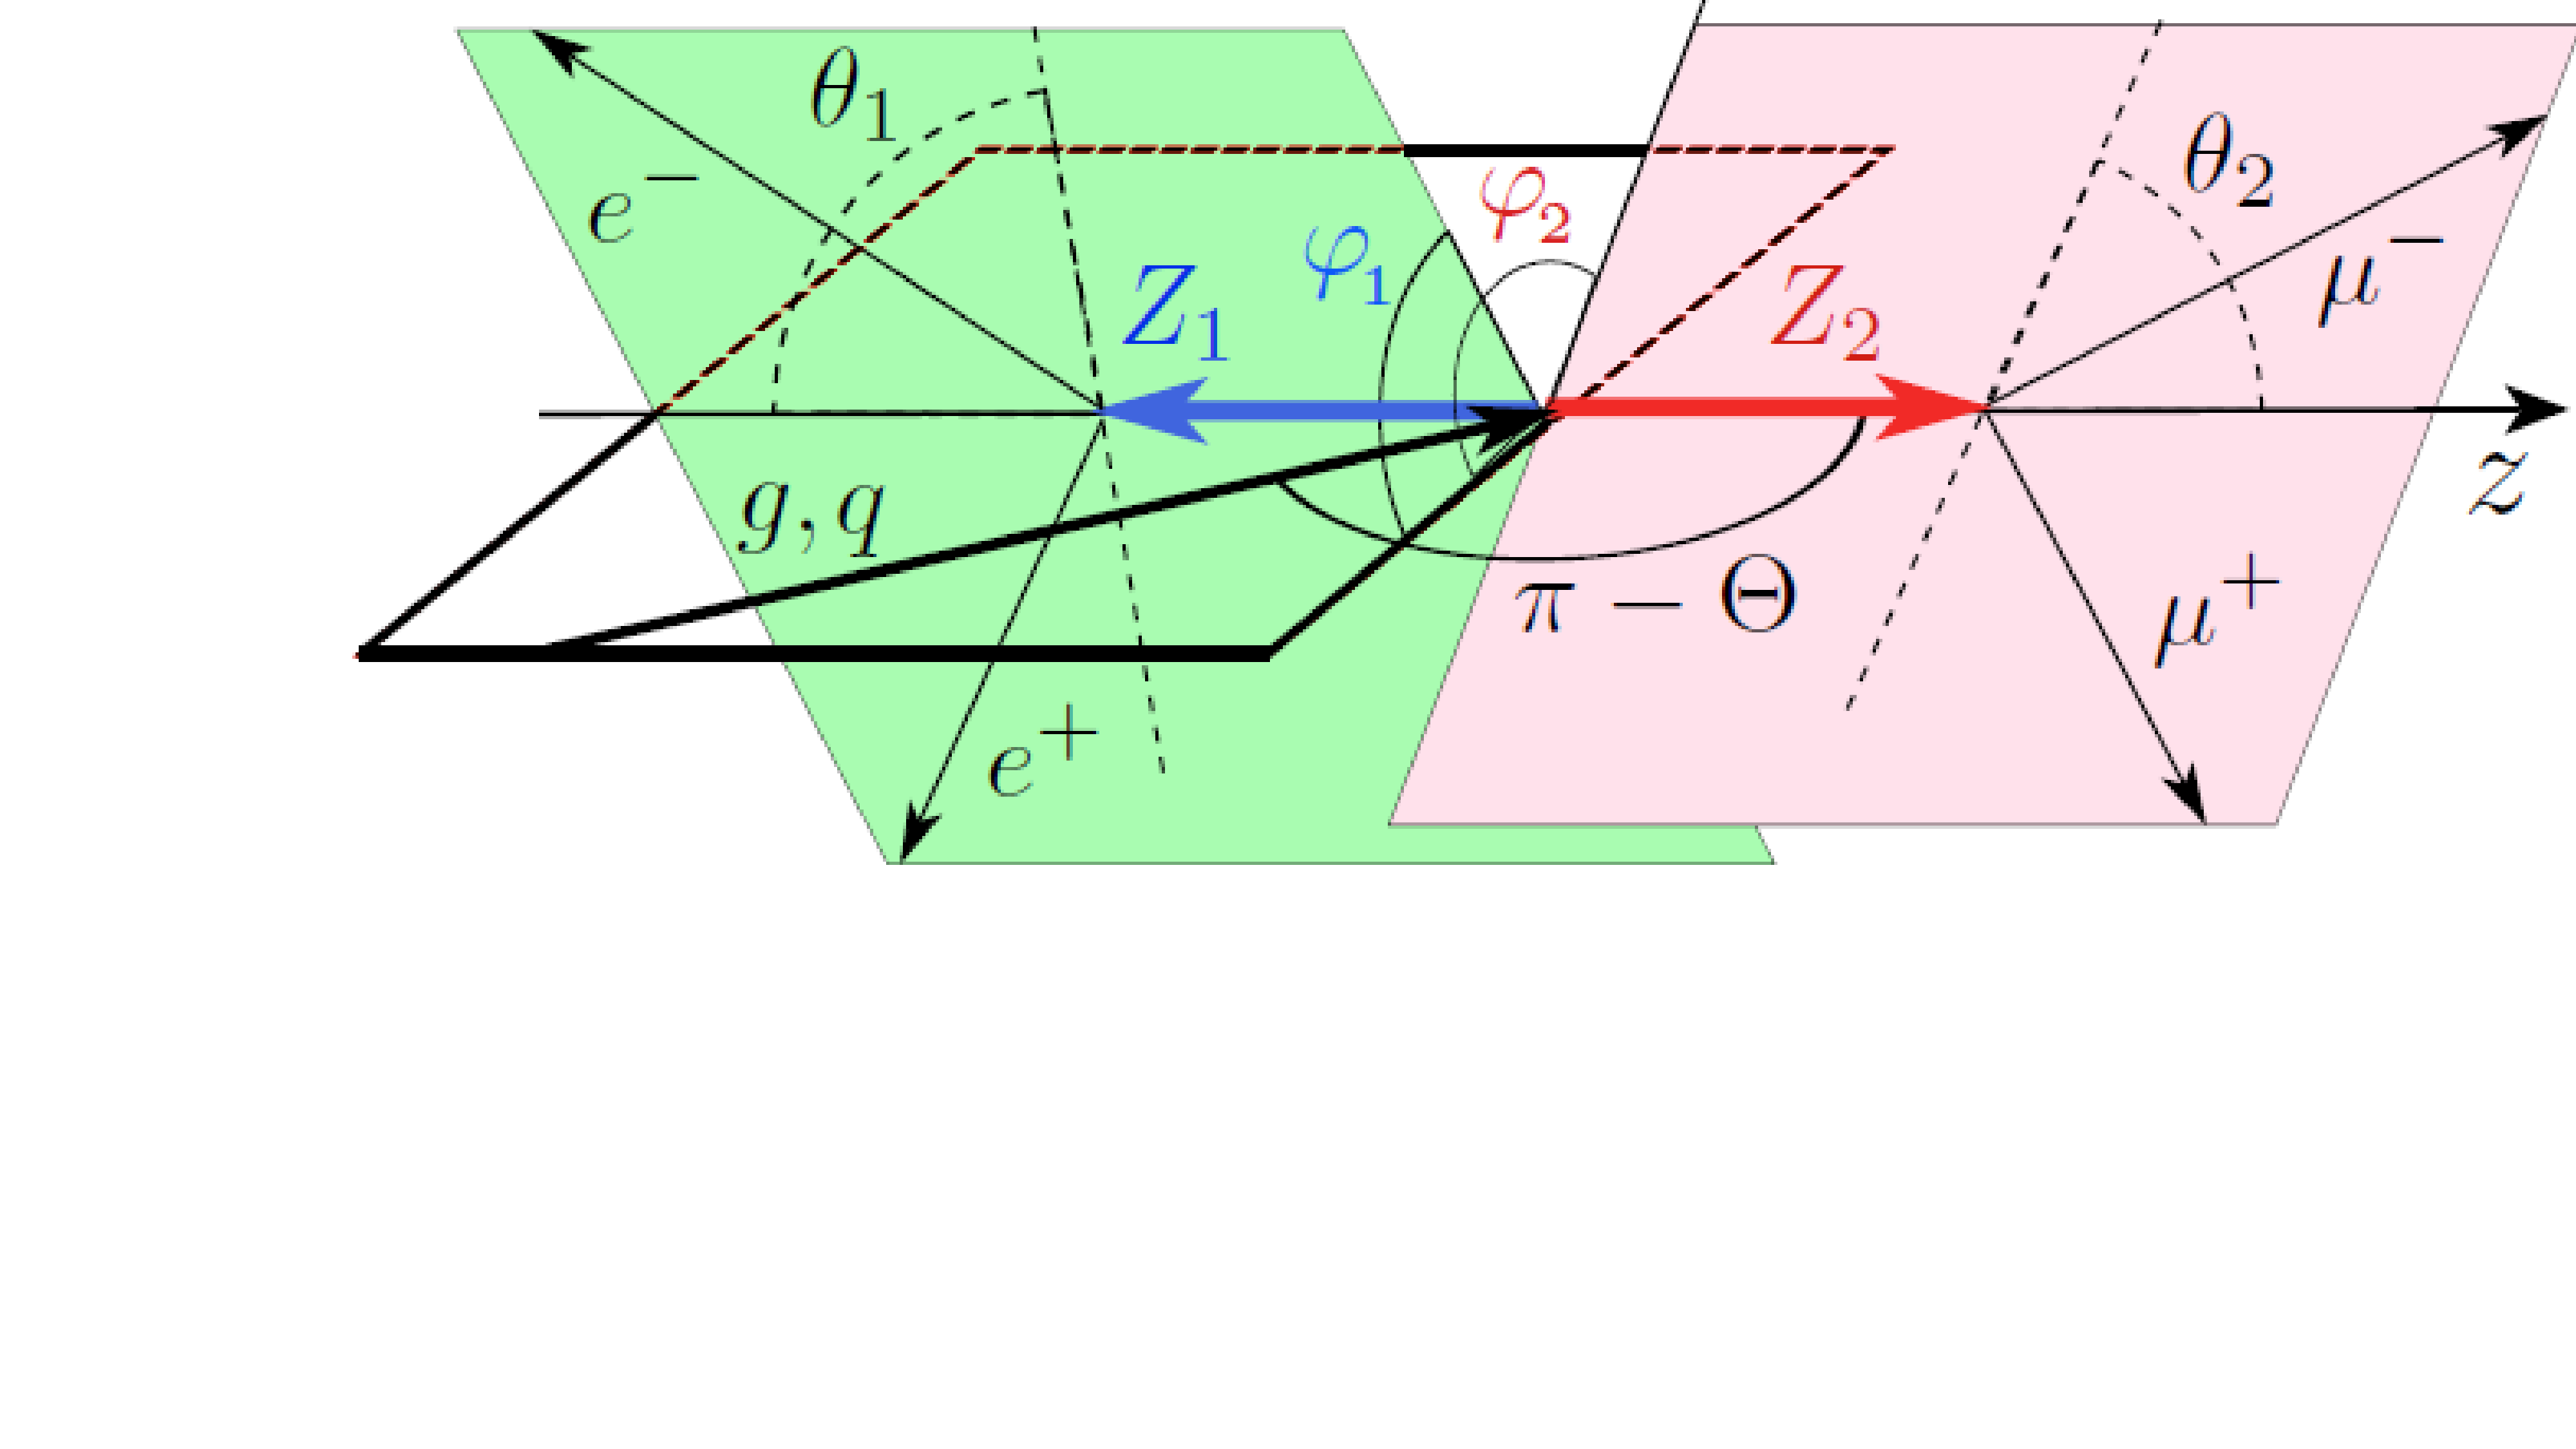
\includegraphics[width=0.85\textwidth]{figures/HiggsSystemDiagram.pdf}
    \caption{ The Cabibbo-maksymowicz angles that fully define the \HiggsToZZ\ system.
    }  
    \label{fig:HiggsSystemDiagram}
  \end{center}
\end{figure}

These angles are diagramatically represented by Figure \ref{fig:HiggsSystemDiagram}.
It's also worth noting that in the case of non-zero spin, there is one more angular degree of freedom.
In such cases, a rotation of the entire system about the axis defined by the direction of the 
Higgs, denoted by $\phi_{\mathrm{H}}$, is no longer a symmetry. 
The typical assumption that it is uniformly distributed is no longer accurate and should be
taken into account in the matrix element calculation. 
When we attempt to simulate detector effects, however, this 6'th angle must always be taken into account,
since Higgs direction might not align exactly with detector.

\subsection{ME expression from Roberto}

Expression for Higgs signal and pseudoscalar Higgs-like signal are taken from paper by Chris et al. (CITE ME)
The general expression for standard model ZZ/ZGamma/GammaGamma background is calculated by Roberto
Mega-Vorales (CITE ME), which includes full interference effects from t/u channels as well as
s-channel single Z production, where one of the leptons radiate an off-shell Z which subsequently decays into
two leptons.  The expression themselves are given both in terms of lepton 4-vectors and CM variables
(angles and masses).  It's too long (>160000 lines) so we don't copy it here.

List of constants used in the expression is listed as follows

\begin{enumerate}
\item $\pi = 3.141592653589793238462643383279502884797169399375105820974944$
\item $M_Z = 91.1876$~GeV
\item $\Gamma_Z = 2.4952$~GeV
\item $\sin^2(\theta_W) = 0.2397$
\item $\alpha_{EM} = \dfrac{1}{127}$
\item $e = \sqrt{4\pi\alpha_{EM}}$
\item $\eta = \dfrac{2 c_v v_a}{c_v^2 + c_a^2} \simeq 0.15$
\item Left-handed coupling to lepton:
   $g_L = 2\left(-\dfrac{1}{2}+\sin^2(\theta_W)\right)\sqrt{\dfrac{\pi\alpha_{EM}}{\sin^2(\theta_W)\cos^2(\theta_W)}}$
\item Right-handed coupling to lepton:
   $g_R = 2 \sin^2(\theta_W)\sqrt{\dfrac{\pi\alpha_{EM}}{\sin^2(\theta_W)\cos^2(\theta_W)}}$
\item Left-handed coupling to up-type quark:
   $g_L^u = 2\left(\dfrac{1}{2}-\dfrac{2}{3}\sin^2(\theta_W)\right)\sqrt{\dfrac{\pi\alpha_{EM}}{\sin^2(\theta_W)\cos^2(\theta_W)}}$
\item Right-handed coupling to up-type quark:
   $g_R^u = 2\left(-\dfrac{2}{3}\sin^2(\theta_W)\right)\sqrt{\dfrac{\pi\alpha_{EM}}{\sin^2(\theta_W)\cos^2(\theta_W)}}$
\item Left-handed coupling to down-type quark:
   $g_L^d = 2\left(-\dfrac{1}{2}+\dfrac{1}{3}\sin^2(\theta_W)\right)\sqrt{\dfrac{\pi\alpha_{EM}}{\sin^2(\theta_W)\cos^2(\theta_W)}}$
\item Right-handed coupling to down-type quark:
   $g_R^d = 2\left(\dfrac{1}{3}\sin^2(\theta_W)\right)\sqrt{\dfrac{\pi\alpha_{EM}}{\sin^2(\theta_W)\cos^2(\theta_W)}}$
\item $v_H = 246$~GeV
\end{enumerate}

\subsection{Formation of the likelihood}

The likelihood we want to calculate depends on the angles, Z candidate masses and Higgs mass.
Once the 5 (+1) angles, Z candidate masses, Higgs mass and Higgs momentum are specified,
the whole system is unambiguously defined.  The description of this system is fully specified by
the differential cross section $d\sigma (\vec{X}, p_T^H, y^H, m_H)$. As a simplification, 
we typically work with the dimensionless equivalent probability density function 
$d\sigma / \sigma = P(\vec{X}_{reco}, p_T^H, y^H, m_H)$. Due to larger theoretical systematic uncertainties from higher order
$\alpha_{\mathrm{s}}$ corrections, we typically do not make use of the differential distribution
in $p_{T}^{H}$ and $y^H$. Instead, we choose to integrate over the best prediction of these
distributions. Thus the expression for the probability density function of interest, 
$P(\vec{X}, m_H)$, where $\vec{X}$ denotes the five angles
and two Z candidate masses, can be expanded in the following fashion:

\begin{eqnarray}
\label{eqn:PDF}
P(\vec{X}_{reco}, m_H) &=& \int_{p_T^H,y^H} P(\vec{X}_{reco}, p_T^H, y^H, m_H)\, \mathrm{d}p_{T}^{H}\, \mathrm{d}y^{H}  \nonumber\\
   &=& \int_{p_T^H,y^H} P(\vec{X}_{reco}, p_T^H, y^H | m_H) \, P(m_H)\, \mathrm{d}p_{T}^{H}\, \mathrm{d}y^{H} \nonumber\\
   &=& \int_{p_T^H,y^H} P(\vec{X}_{reco} | p_T^H, y^H, m_H) \, P(p_T^H, y^H | m_H) \, P(m_H)\, \mathrm{d}p_{T}^{H}\, \mathrm{d}y^{H},
\end{eqnarray} 

where the probability density function for $\vec{X}_{reco}$, $p_T^H$, $y^H$, and $m_H$ can be factorized into a
product of conditional probability density functions $P(\vec{X}_{reco} | p_T^H, y^H, m_H)$, $P(p_T^H, y^H | m_H)$, and $P(m_H)$.
Then, we express the conditional probability density function $P(\vec{X}_{reco} | p_T^H, y^H, m_H)$, $P(p_T^H, y^H | m_H)$
as a convolution of the matrix element computed at particle level with the transfer functions that take particle level
four-momenta into the reconstructed four-momenta:

\begin{eqnarray}
\label{eqn:CondPDF}
P(\vec{X}_{reco} | p_T^H, y^H, m_H) &=& N \int_{\vec{X}_{gen}, \phi_{H}} ME(\vec{X}_{gen} | m_H)
      \, \epsilon(\vec{X}_{reco})|_{\phi_H,p_T^H, y^H, m_H} \, F(\vec{X}_{gen}, \vec{X}_{reco})|_{\phi_H,p_T^H, y^H, m_H} \nonumber\\
 &=& N \int_{\vec{X}_{gen}, \phi_{H}} ME(\vec{X}_{gen} | m_H)
      \, \epsilon(\vec{X}_{reco})|_{\phi_H,p_T^H, y^H, m_H} \, F(\vec{X}_{gen}, \vec{X}_{reco})|_{\phi_H,p_T^H, y^H, m_H}, \nonumber\\
\end{eqnarray} 

where $N$ is some constant which properly normalizes the probability density function.
The function $ME(\vec{X}_{gen} | m_H)$ is the matrix element and depends only on the particular hypothesized quantum numbers 
of the Higgs candidate. It is independent of the Higgs candidate momentum. The function $\epsilon(\vec{X}_{reco})|_{\phi_H,p_T^H, y^H, m_H}$
describes the product of the acceptance and lepton selection efficiency, whereas $F(\vec{X}_{gen}, \vec{X}_{reco})$
is the transfer function that takes the particle level $\vec{X}_{gen}$ to the reconstructed level $\vec{X}_{reco}$.


The Higgs candidate transverse momentum and rapidity spectrum $P(p_T^H, y^H | m_H)$ is obtained 
from generator-level information.  Several generators are used to generate the spectrum: 
MC@NLO (version 4.07) interfaced with {\sc Herwig++} (version 2.6.0).
% POWHEG+Pythia?? <== for signal this will be one of the alternate map for systematics %
In the case of standard model ZZ background, the $p_T$ and $y$ refer to the 
transverse momentum and rapidity of the di-boson system
This spectrum is currently computed using {\sc Powheg} (revision 2119)
interfaced with {\sc Pythia8} (version 8.165). %let's consider checking against POWHEG%

The acceptance is computed for the lepton $p_{T}$ and $\eta$ cuts and the cuts on the
masses of the two Z candidates that were applied for the ICHEP 2012 analysis simply
by evaluating how many generated events with a given system configuration pass such cuts. 
The lepton selection efficiency is evaluated using the Monte Carlo simulation as described
in Section \ref{sec:EfficiencyModel}.

Due to the multi-dimensional nature of the probability density functions, we are 
sensitive to the computational time needed to perform the integrations. 
To reduce computational time, we assume that the resolution on the direction of the 
lepton trajectory is negligible. From the Monte Carlo simulation, we observe that
the angular resolution for the direction of leptons is typically significantly below 
a percent, so that neglecting this effect is a fairly good approximation. 
Therefore, we only account for the resolution on the momentum of the leptons.
The transfer function can be written as:

\begin{eqnarray}
F(\vec{X}_{gen}, \vec{X}_{reco}) &=& \delta (\Theta_{gen} - \Theta_{reco})
   \delta (\Phi_{gen} - \Phi_{reco})
   \delta (\phi_{gen} - \phi_{reco})
   \delta (\theta_{1, gen} - \theta_{1, reco})
   \delta (\theta_{2, gen} - \theta_{2, reco}) \nonumber\\
   &\,& F(m_{1, gen}, m_{2, gen}, m_{1, reco}, m_{2, reco}), 
\end{eqnarray}

and reduces to a transfer function for the masses. This transfer function is 
evaluated using the binned resolution functions of each lepton described
in section \ref{sec:MomentumResolutionModel}. As a simplification, 
we suppress the effect of the lepton momentum resolution on $m_H$.  
Note that interchanges between the two Z candidates 
is also taken into account, if the lower Z candidate mass fluctuates
above the higher one.


\subsection{Binned Representation of the likelihood}

The probability density functions in Equations \ref{eqn:PDF}
and \ref{eqn:CondPDF} are defined in terms of a large number of integration. These integrals 
cannot generically be solved symbolically, and we must instead resort to numerical 
integration techniques. As a result, the finite size of the numerical integration
grid bins define the granularity to which we can define these probability
density functions. Therefore, all of our probability density functions
are represented by binned maps, from here on denoted as $P_B$ to 
distinguish them from $P$ which denote the corresponding continuous representations.

%
% Si: don't really understand the point of the statement below.
% Yi: It's related to BDT approach, since they need MC for training.  Let's delete this paragraph.
%
% Since the bin contents are calculated via theoretical calculations of the matrix element,
% detector effect parameterization and underlying spectrum for the ZZ system,
% and not from generating MC events to populate all bins,
% we can afford to have much large number of binnings without running into problems
% of insuficient statistics.
%

We start by generating conditional maps with fixed $m_H$: $P_B(\vec{X}_{reco} | m_H)$.
The $\phi$ and $\Phi$ angles are binned in uniform steps between 0 and $2\pi$.
The other angles, $\Theta$, $\theta_1$ and $\theta_2$ are binned uniformly
in the cosine of the angle from -1 to 1.
The ``on-shell'' Z candidate mass is binned uniformly from 0 to 110\% of Higgs mass,
and ``off-shell'' Z candidate mass is binned uniformly from 0 to 55\% of Higgs mass.
Current working dimension (number of bins) for these are
12 bins in $\Phi$, 15 bins in $\Theta$, 10 bins in $\phi$, 12 bins in $\theta_1$,
12 bins in $\theta_2$ and 22 bins in both Z candidate masses, resulting
in roughly $125 \times 10^6$ bins per $m_H$.

The integrals in the likelihood expression are evaluated using the Monte Carlo integration technique.
This is done by randomly drawing a sample from the $p_T, y$ two-dimensional spectrum, as well
as $\phi_H$, then calculating the contribution to the likelihood, and then repeating this many times.
For each sampling, we first smear the momentum of the leptons, and then compute the corresponding efficiency and acceptance
via a lookup table using the values given in Section \ref{sec:EfficiencyModel}.
Then we recalculate the Z candidate masses, and fill the result into the correct bin
after multiplying the appropriate matrix element. Since the bins are large, we also randomize the angles and masses from sample
to sample within each bin.

The likelihood is then normalized according to the following condition:

\begin{eqnarray}
\sum_{\vec{X}} P_B(\vec{X} | m_H) \Delta\Phi \Delta\Theta \Delta\phi \Delta\theta_1 \Delta\theta_2
   \Delta m_1 \Delta m_2 &=& 1. 
\end{eqnarray}

Since all the angle bin sizes are constant across the whole analysis,
and in the end we only care about likelihood ratios, we can ignore these factors.
The bin sizes in masses do change across different $m_H$ maps, so we need to
keep them around.  The working normalization condition we chose
in the end is as follows:

\begin{eqnarray}
\sum_{\vec{X}} P_B(\vec{X} | m_H) m_H^2 &=& 1. 
\end{eqnarray}

The last dimension, in $m_H$, is fairly large and it is inefficient to
scan through it with small binning. Instead, we generated conditional 
maps $P_B(\vec{X}_{reco} | m_H)$ for a handful of different Higgs masses, 
and interpolate for intermediate masses.  
The current choice of masses are 100, 110, 120, 125, 130, 140,
160, 200, 300 and 400, for a total of 10 bins.  Computationally
we could afford more bins if we want better discrimination for masses
that are far away from 125.

The interpolation of maps is done bin-by-bin as follows.
First we find the enclosing two maps, and calculate the interpolation:

\begin{eqnarray}
P_B(\vec{X} | m_H)
   = \dfrac{(m_{H_2}^2 - m_H^2) P_B(\vec{X} | m_{H_1}) + (m_H^2 - m_{H_1}^2) P_B(\vec{X} | m_{H_2})}
      {m_{H_2}^2 - m_{H_1}^2},
\end{eqnarray}

assuming $H_1 < H < H_2$.  This interpolation preserves the normalization
condition for all intermediate Higgs masses.

\subsection{Interpolation in the other dimensions}

The computing power is limiting much higher number of bins than what is current used, and
the rather-coarse bin size generates discontinuities in the final likelihood.
In order to mitigate the effect, we have implemented linear interpolations in all
7 dimensions.  The interpolation for any non-cyclic dimension proceeds as follows:

\begin{enumerate}
\item For each bin, take the bin center point as the representative of the bin
\item Connect all the bin centers into a pair-wise linear function
\item For the outermost two bins, the two half of the bin that is not covered
gets a flat value of the bin themselves.
\end{enumerate}

In the case of cyclic dimensions ($\phi, \Phi$),
the pair-wise linear function goes across the border,
connecting center of first bin and center of last bin.

This choice of interpolation perserves total integral of the 7D map, and therefore
there is no need to recalculate it.

To combine the interpolation for multiple dimensions, we follow a simple generalization
from linear $\rightarrow$ bilinear $\rightarrow$ trilinear interpolation:
interpolate dimensions one by one.  The order doesn't matter, since it's linear.

Side note...this is non-trivial to implement, especially with more than 1B bins
and one does not simply load everything into memory.
Should I include description of the implementation?
Maybe none of the physicists will be interested though.
Let's leave that aside for now.


\subsection{Uncertainty bin-by-bin due to numerical integration}

TODO Repeat exercise and fill in

\subsection{Toy generation and hypothesis testing without systematic uncertainties}

In order to study expected signal-to-background separation, we developed
an algorithm to efficiently generate large amounts of pseudo-data.
From above, we already have the expression of $P_B(\vec{X}|m_H)$,
which is an approximation of the continuous probability density function
$P(\vec{X}|m_H)$.  To generate pseudo-experiments, $P(m_H)$ is needed
as input.

The basic steps of toy generation is as follows:

\begin{enumerate}
\item For each new sample, determine the values of $\vec{X}$
from the ensemble of conditional maps.  This step will be
elaborated more in the next paragraph.
\item Once we know $\vec{X}$, we can look up the maps and get a
1D distribution of $m_H$ by multiplying a piece-wise linear
interpolated function and the input $P(m_H)$.
\item Finally, from this 1D distribution we determine what
the value of $m_H$ that we want for the sample.
\item Return to step one as many times as needed, and collect the output.
\end{enumerate}

This procedure has some shortcomings in the case of huge maps
that we are dealing with.  First, There are more than $10^9$
bins in total, and random access to this map is very time-consuming.
Furthermore, typically we need a huge number of generated samples too,
which worsens the problem.  We also need to do quite some pre-processing
to integrate out $m_H$ and get the correct $P_B(\vec{X})$
for the first step.  To get around this problem,
the algorithm is reassembled, taking advantage of the Poisson nature of
toy generation:

\begin{enumerate}
\item Specify target number of toy samples we want in the end.
\item Loop over $\vec{X}$, for each bin we calculate target number of toy samples that
will fall into this bin.
\item Make a decision on the actual number of events that will be generated from this bin by
drawing a number from a Poisson distribution centered at the target sample count
\item Generate toy(s) from this 1D $m_H$ distribution.
\item After looping through all bins, randomize the order of the generated samples.
\end{enumerate}

For this modified algorithm, we only need to loop through the map once.
If we want to calculate normalization on the fly, then we need to loop through the map twice.
Random access to the map is not needed either.  The slight
inconvenience is that actual number of generated events might not be exactly
what we wanted, but this can be easily compensated by generating more events
then needed in the end and randomly discard some of them.


TODO Recap of likelihood normalization, condition for $P(m_H)$

TODO Result of separation.

\subsection{7TeV vs. 8TeV}

TODO Generate map with 7 TeV spectrum, and compare distance

\subsection{Projection to different amount of data}

This section will be moved later

This part will come later

\section{General Scalar Lagrangian}

In addition to the specific hypotheses introduced before, we have also received the expression of general
Lagrangian for spin-0, including full interference effects.  The relevant parts of Lagrangian is as follows:

\begin{eqnarray}
\mathcal{L} &=& A_1^{ZZ} m_Z^2 X Z_\mu Z^\mu + A_2^{ZZ} X Z_{\mu\nu} Z^{\mu\nu} + A_3^{ZZ} X Z_{\mu\nu} \tilde{Z}^{\mu\nu} \nonumber\\
   &+& A_1^{ZA} (\textrm{1 GeV})^2 X Z_\mu A^\mu + A_2^{ZA} X Z_{\mu\nu} F^{\mu\nu} + A_3^{ZA} X Z_{\mu\nu} \tilde{F}^{\mu\nu} \nonumber\\
   &+& A_1^{AA} (\textrm{1 GeV})^2 X A_\mu A^\mu + A_2^{AA} X F_{\mu\nu} F^{\mu\nu} + A_3^{AA} X F_{\mu\nu} \tilde{F}^{\mu\nu},
\end{eqnarray}

where the coefficients $A_i^{XX}$ are dimensionless coupling strengths.  For the expression I have, $A_1^{ZA}$ and
$A_1^{AA}$ are always set to zero for some reason I don't quite understand.  Sure, direct terms like that violates
gauge symmetry, but if this is an effective theory, I'm not sure why we can't have terms like that.  Anyways.
Each non-zero coefficients are allowed to be complex, so there are 14 coefficients to specify to use the expression.

\subsection{Relative strength of different terms}

The relative strength of the terms can be estimated by looking at the integrals.  Since the coupling constans are all
unitless, and we're only interested in relative strength of the terms, we are free to choose whatever coupling we want.
For ths purpose of visualizing the size of interference terms, I choose coupling constants so that each of the
pure terms (ie., when there's only one term in the Lagrangian) has the same integral as the other.  Under this choice
of parameters, we can integrate various interference terms and see how large they are.  I have tried two different
way of integrating the expressions; either integrating the expression directly, or integrating the absolute value
of the expressions, since interference terms tend to be partly constructive and partly destructive, as illustrated for
example in Figure \ref{fig:A1A3PhiDistribution}, where we compared $A_1^{ZZ}$ and $A_3^{ZZ}$ and their interference.

\begin{figure}[htb!]
  \begin{center}
    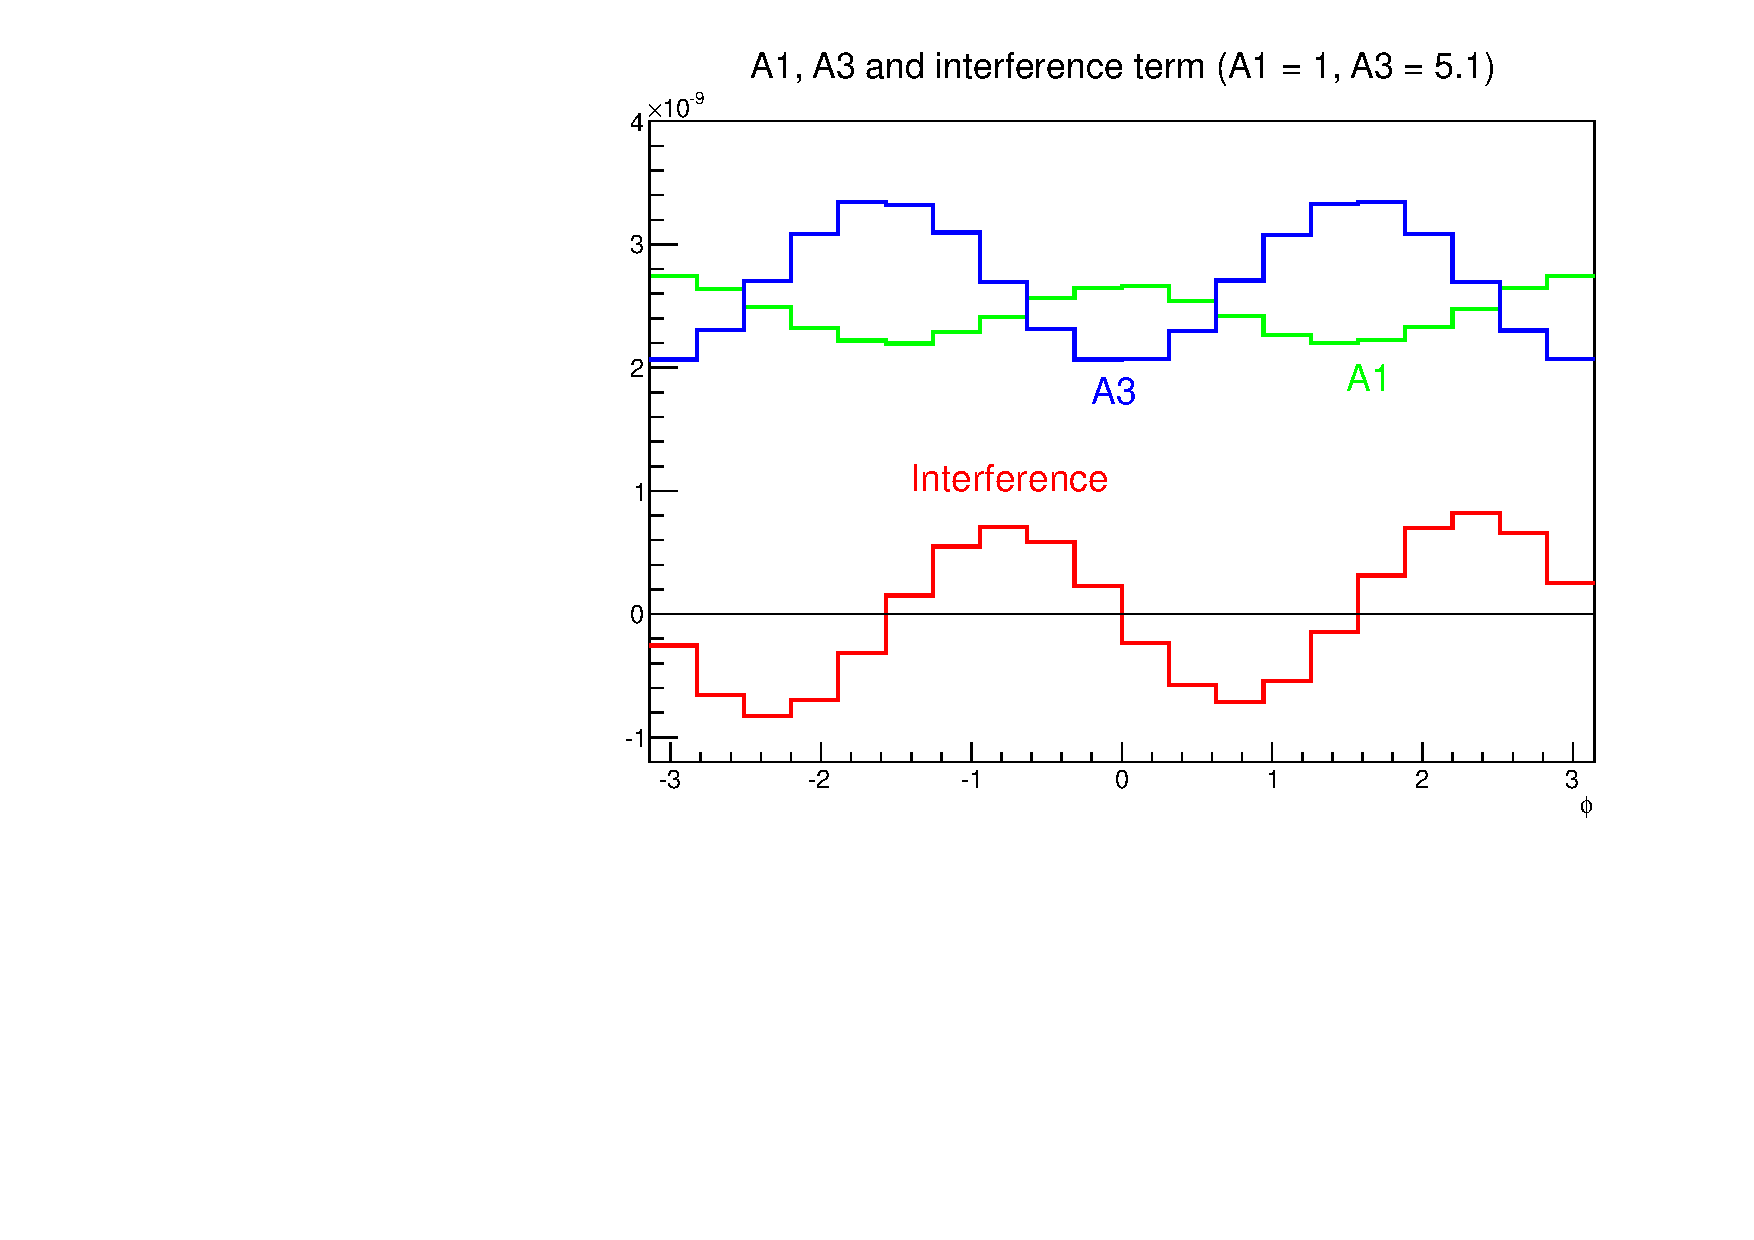
\includegraphics[width=0.48\textwidth]{figures/SignalPhiComparison.pdf}
    \caption{Comparison of $A_1^{ZZ}$ and $A_3^{ZZ}$ with their interference, when the two terms are
    roughly of the same size.  This is for $M_H = 125$ GeV.}
    \label{fig:A1A3PhiDistribution}
  \end{center}
\end{figure}

Summary plots are shown in Figure \ref{fig:InterferenceSize}.  Plots for different $M_H$ values are shown.
We apply basic phase-space cuts to be closer to real experimental analysis: $40 < M_1 < 120$ and $10 < M_2 < 120$.
For each plot, the diagonal entries are the pure terms, and they equal to 1 by construction, since this defines
the choice of parameters.  The off-diagonal terms are all various interference terms.  Each parameter appears
twice in both the x axis and y axis with real and imaginary components.  The plots can be divided into
quadrants.  The lower-right quadrant is empty so let's ignore those.  Lower-left quadrant is the case
when all parameters are real, and the upper-right quadrant is the case when all parameters are pure imaginary.
These two triangles are exactly the same since we don't expect to be sensitive to overall phase shifts.
Here we can already see that the interference terms are partly constructive and partly destructive, and
the absolute value integral is by no means negligible compared to the pure terms.
The upper-left quadrant is the interference between real component and imaginary components.
Supposedly this is the only place where we might have CP violation (need to check with people).

\begin{figure}[htb!]
  \begin{center}
    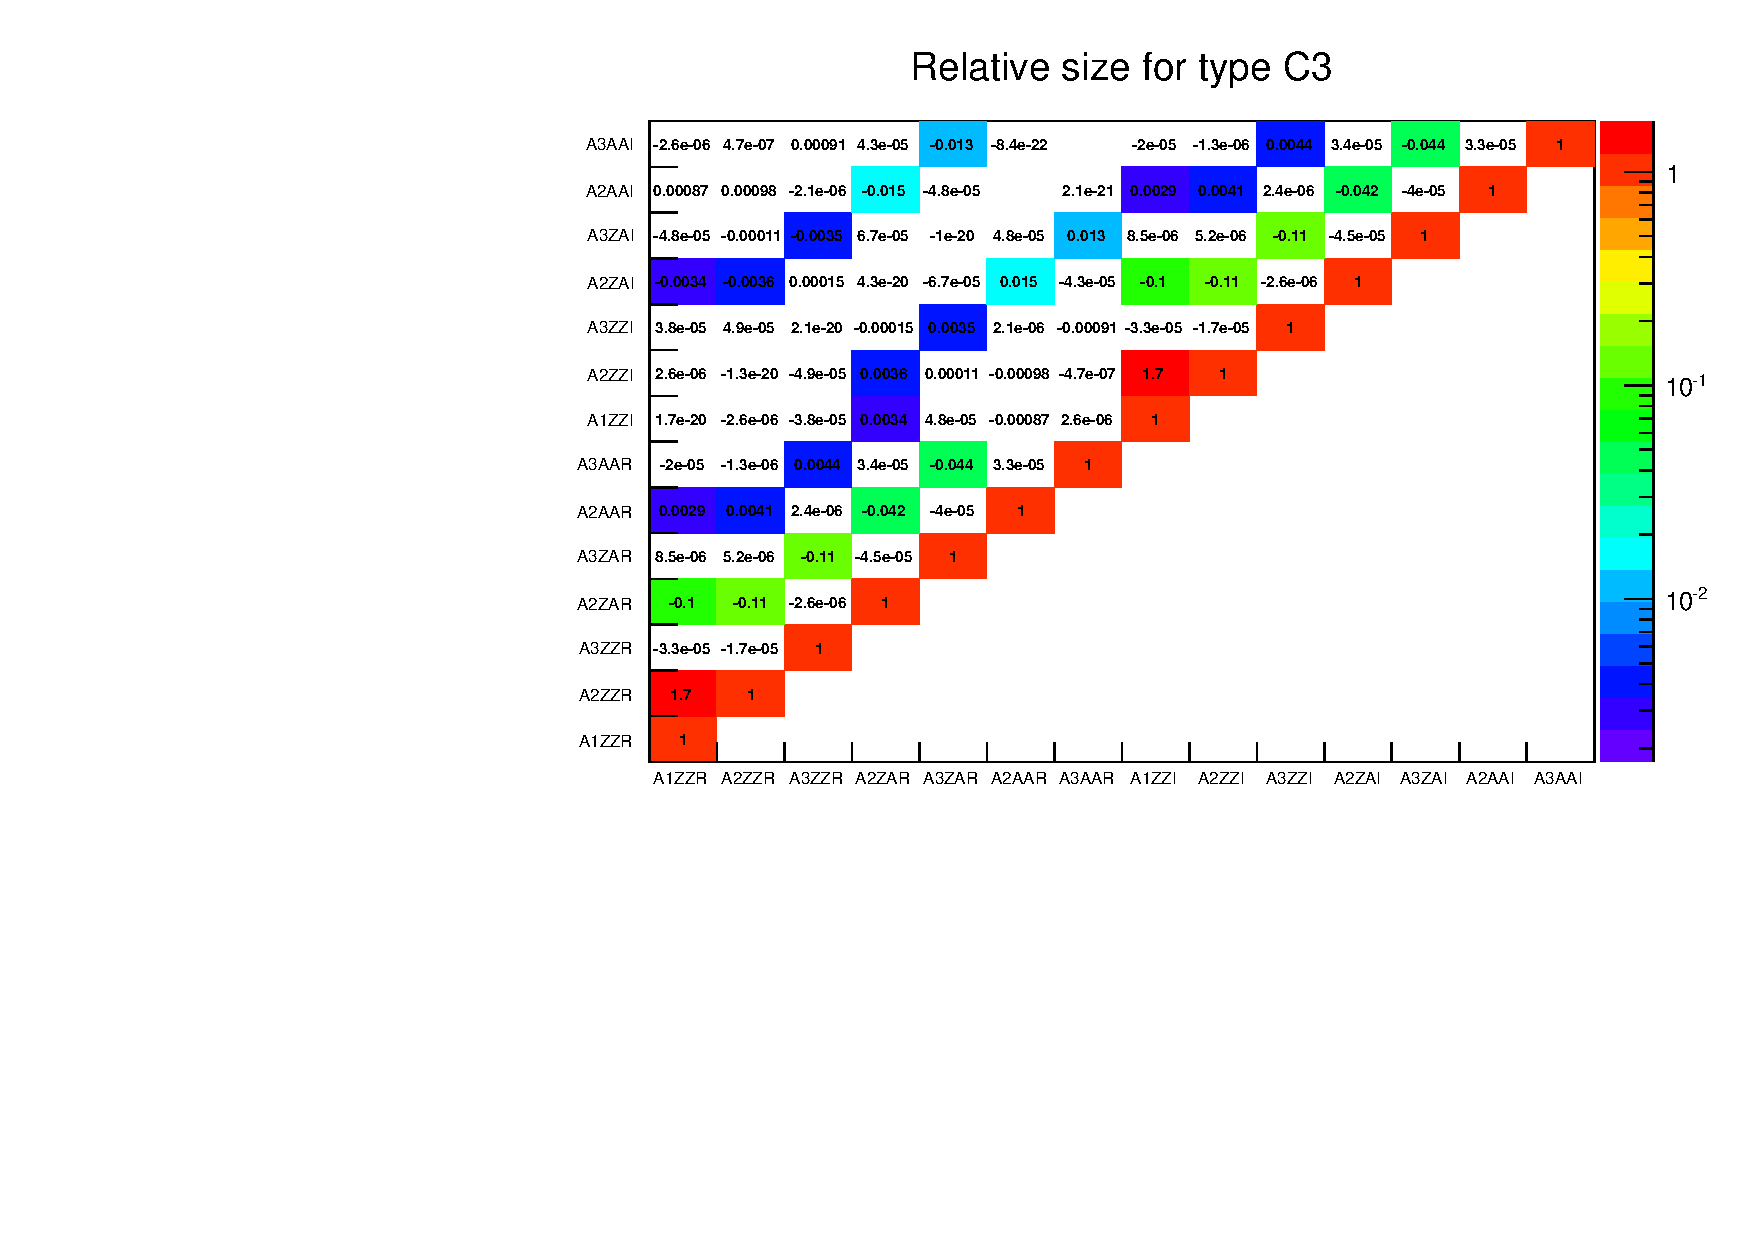
\includegraphics[width=0.48\textwidth]{figures/InterferenceSizeUsualIntegral_C3.pdf}
    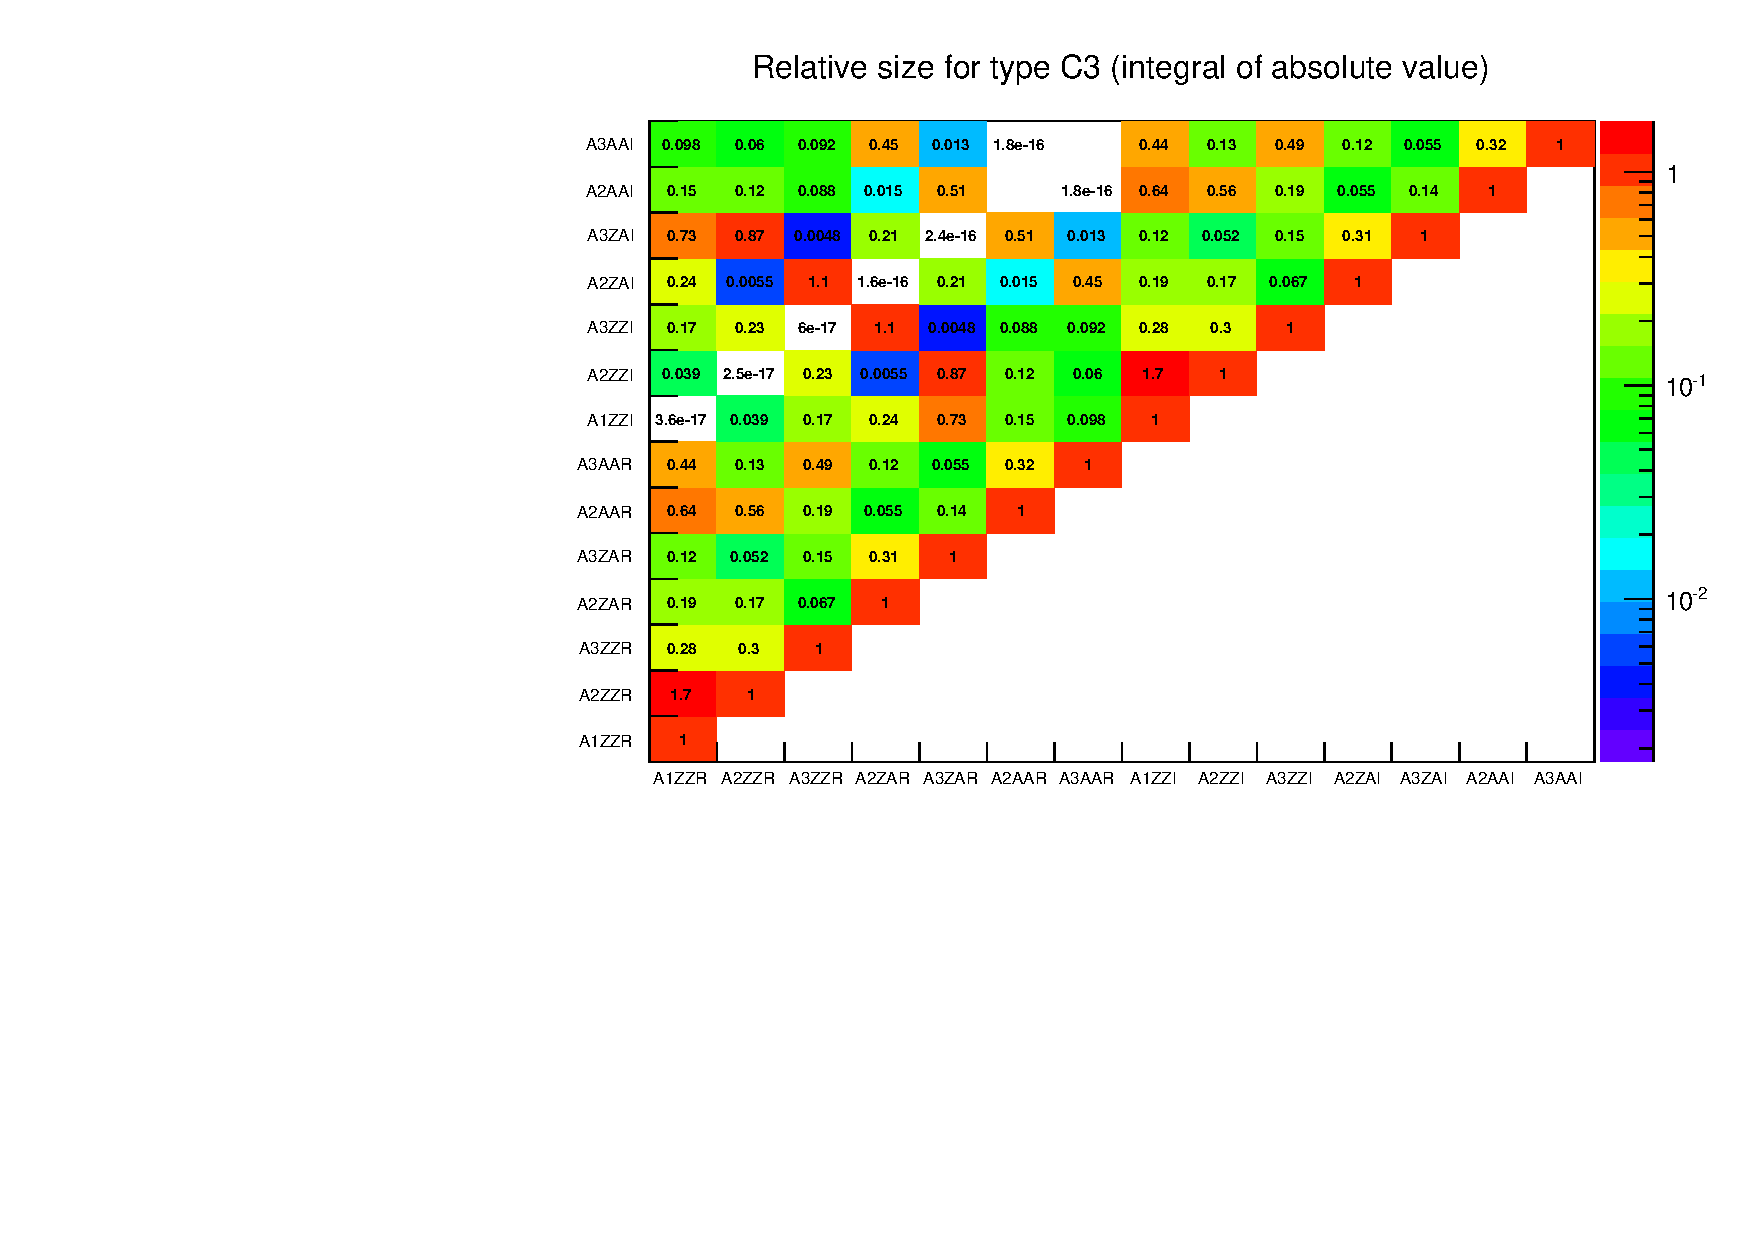
\includegraphics[width=0.48\textwidth]{figures/InterferenceSizeAbsoluteIntegral_C3.pdf}\\
    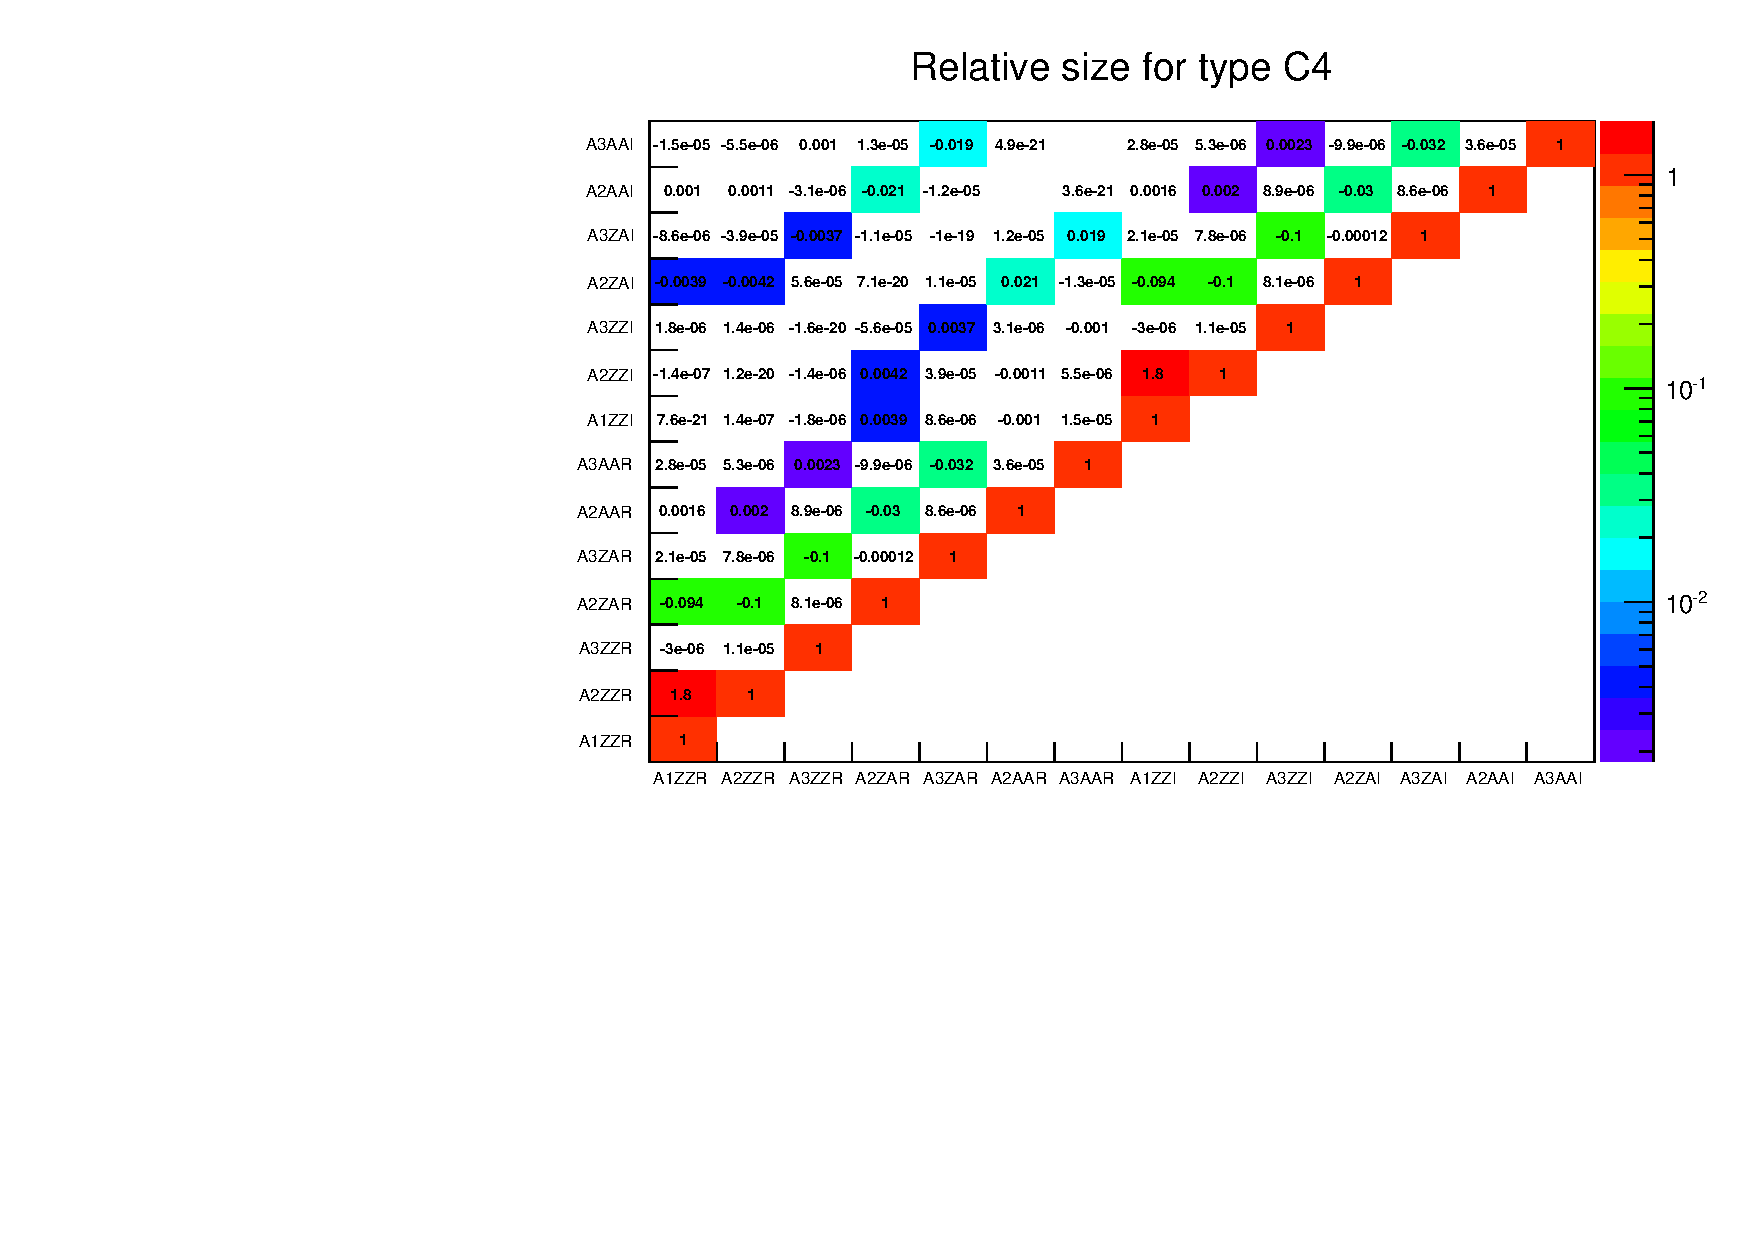
\includegraphics[width=0.48\textwidth]{figures/InterferenceSizeUsualIntegral_C4.pdf}
    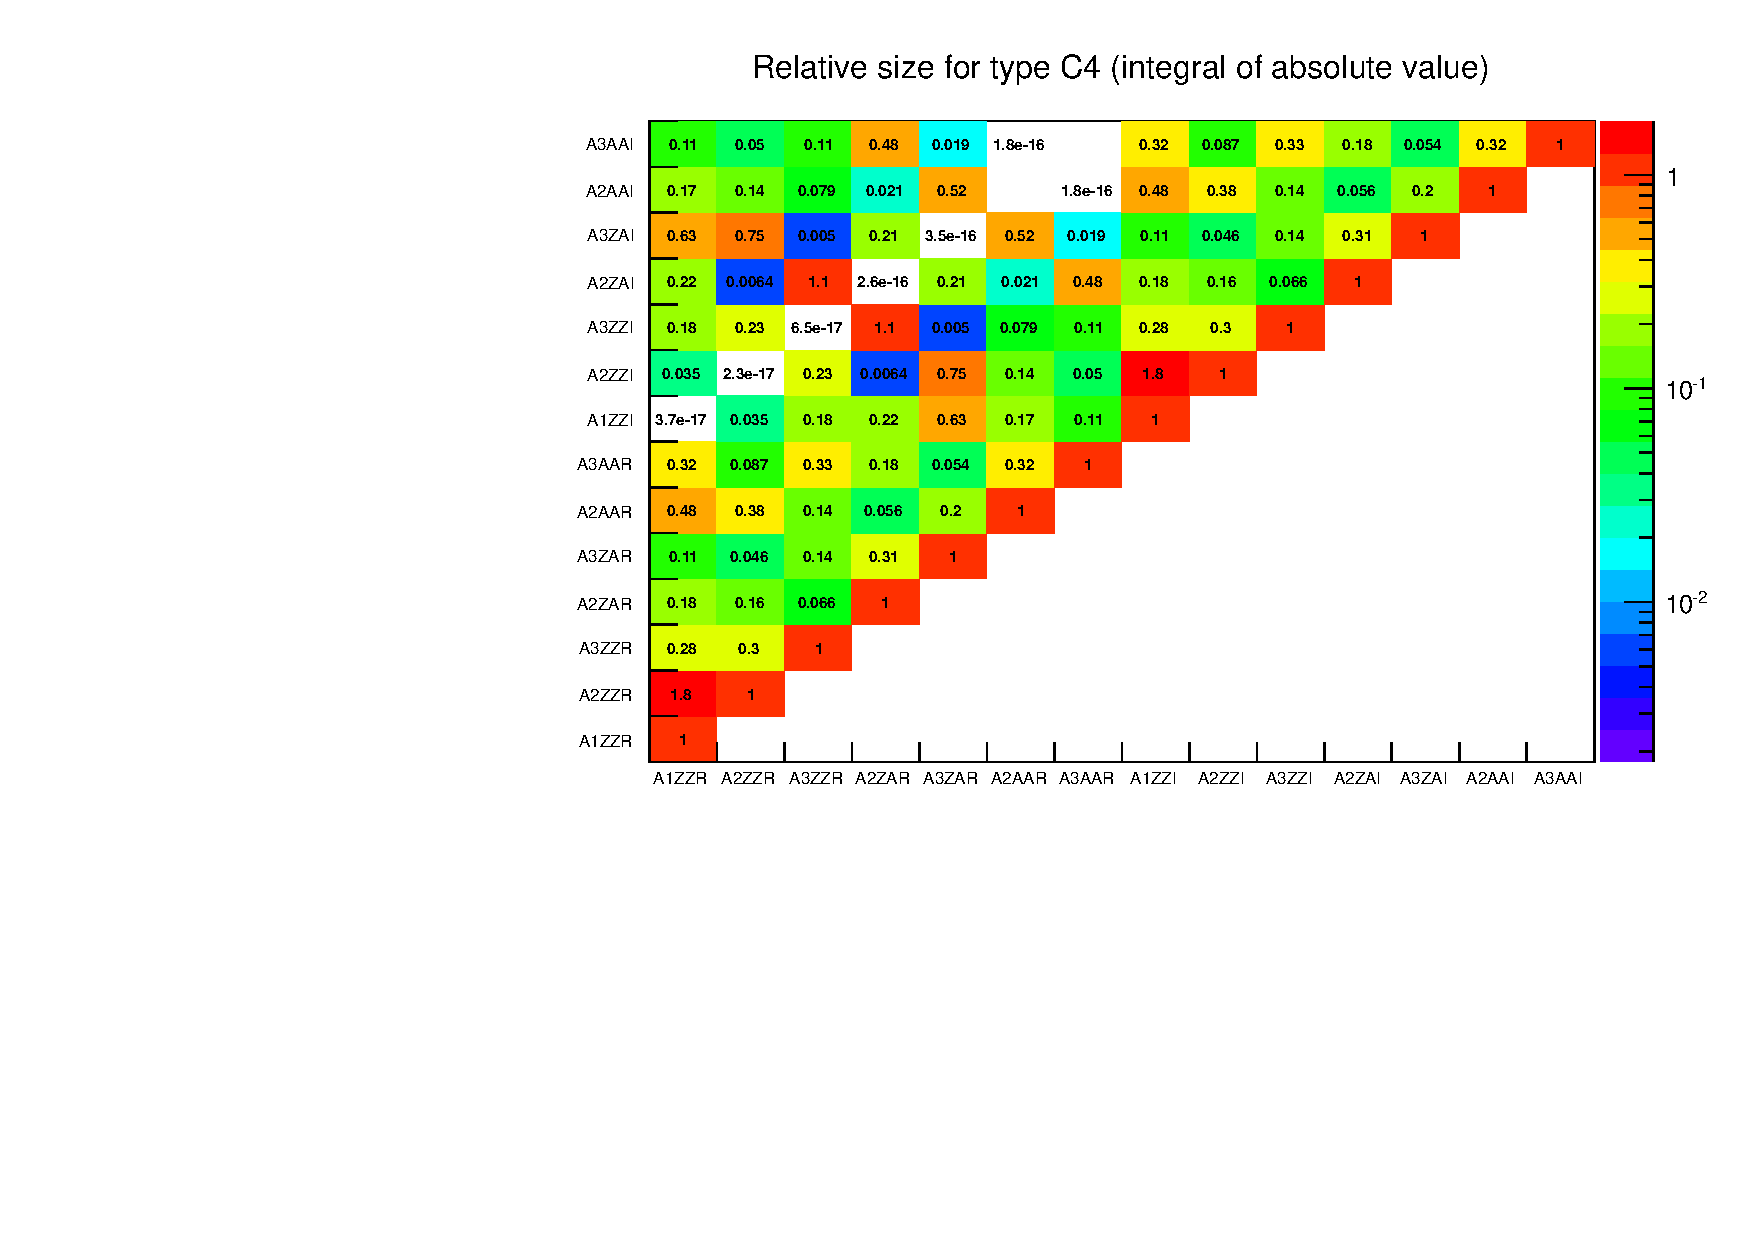
\includegraphics[width=0.48\textwidth]{figures/InterferenceSizeAbsoluteIntegral_C4.pdf}\\
    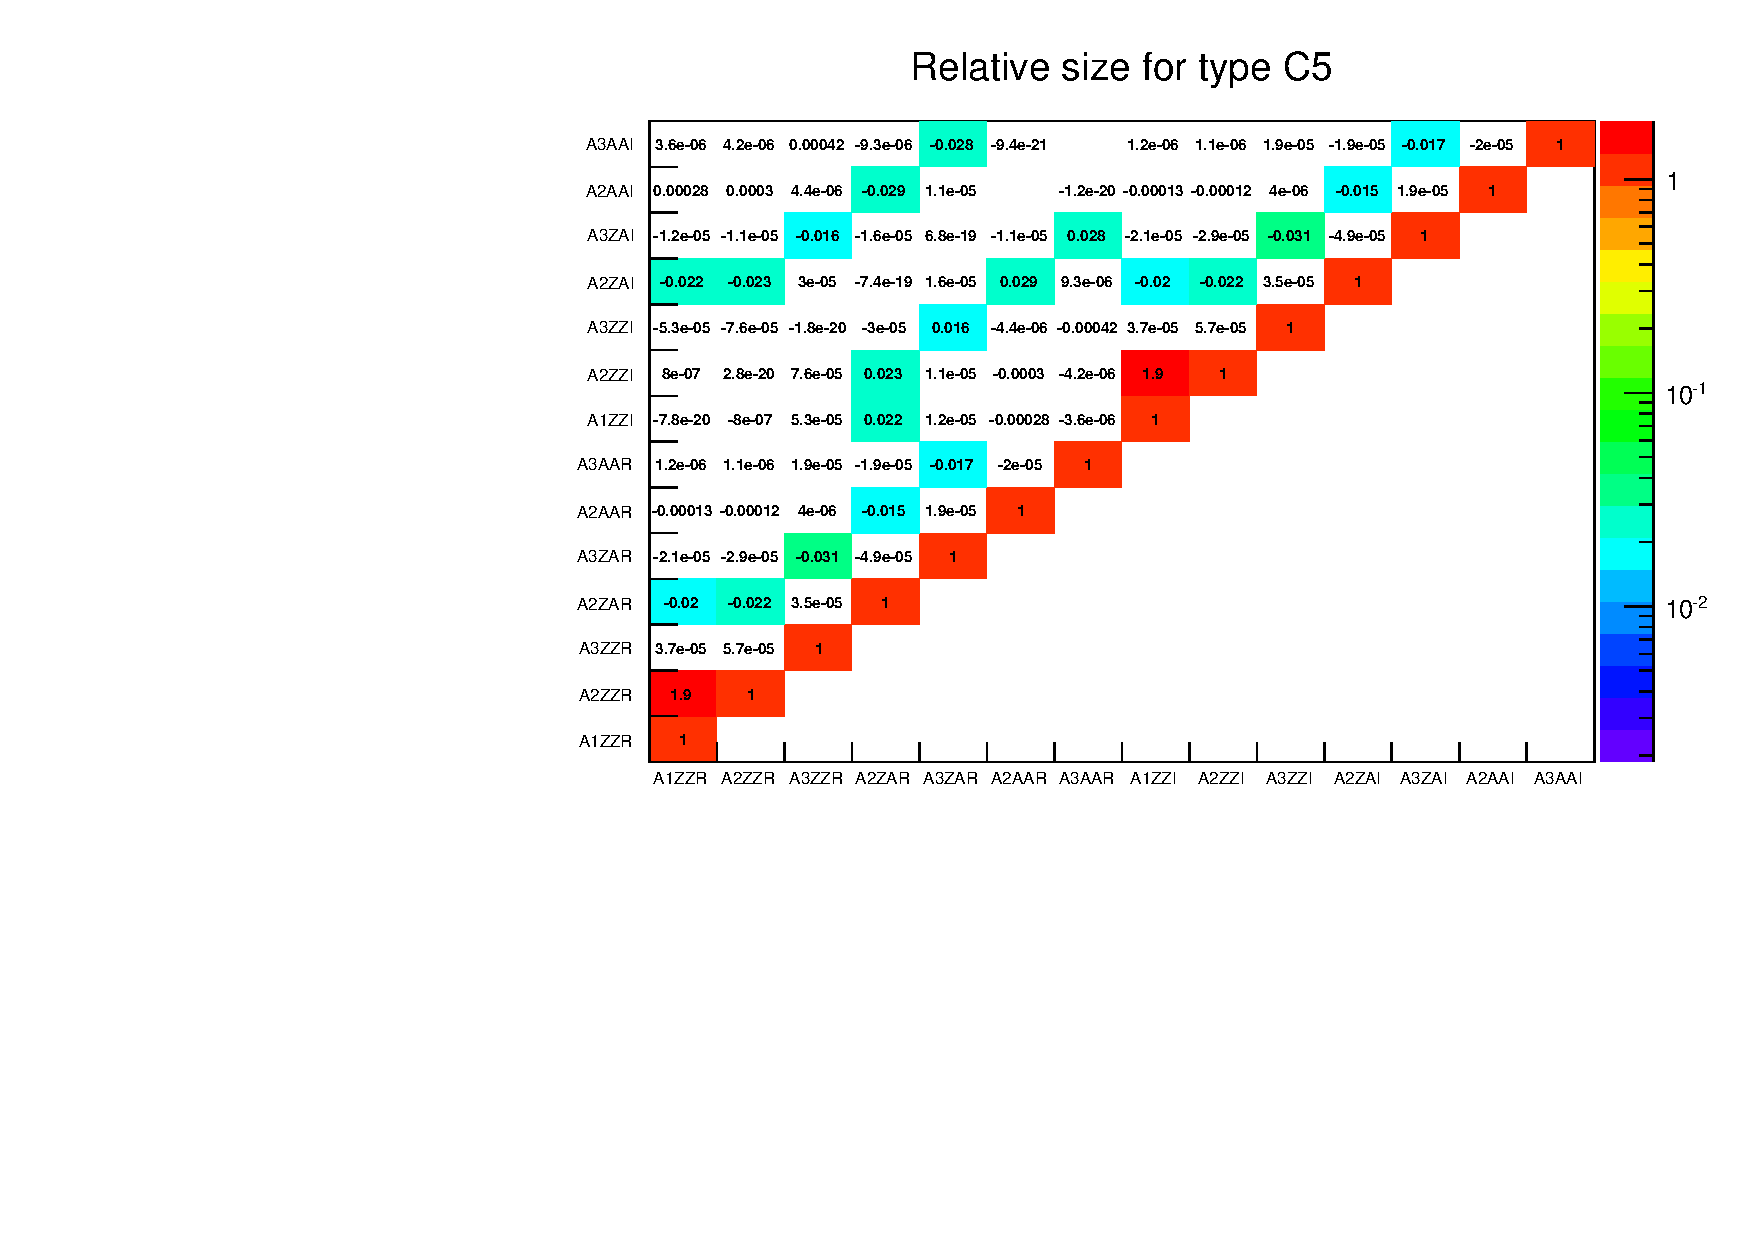
\includegraphics[width=0.48\textwidth]{figures/InterferenceSizeUsualIntegral_C5.pdf}
    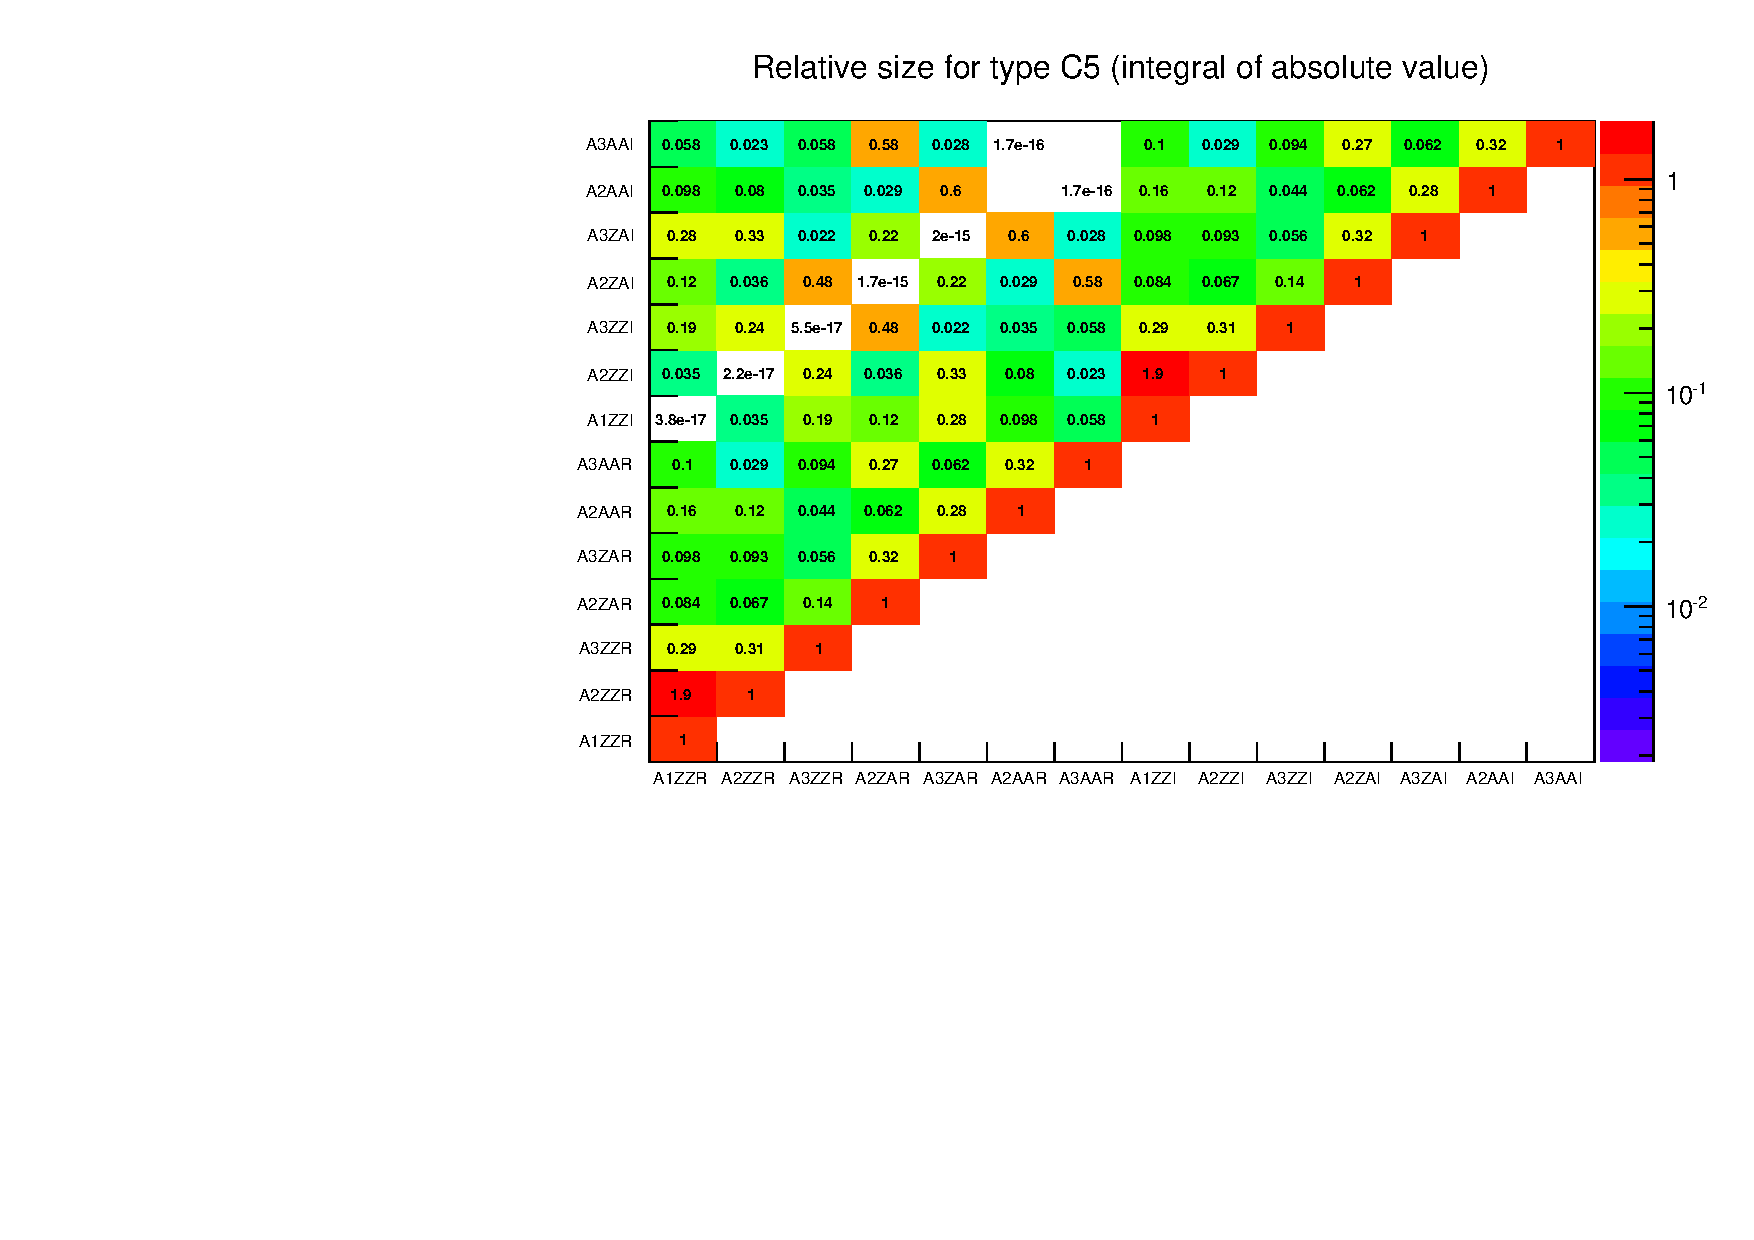
\includegraphics[width=0.48\textwidth]{figures/InterferenceSizeAbsoluteIntegral_C5.pdf}\\
    \caption{Size of interference terms when all pure terms have the same size for $M_H = 125, 145$ and 200 GeV.
    The three rows are for different $M_H$, and left column is usual integral, right column is the integral of
    absolute values.  (n.b. I will fix plot title later - C3 = 125 GeV, C4 = 145 GeV, C5 = 200 GeV; and they all have phase space cut of M1 = 40-120, M2 = 10-120.  I might switch it to D3-D5 later, where there's extra requirement on 5 GeV leptons, but the plot doesn't change much with the lepton pt cuts.)}
    \label{fig:InterferenceSize}
  \end{center}
\end{figure}



\section{Fitting}

\subsection{Methods: how to fit - 7D}

We have performed maximum-likelihood fits to say something about
the parameters of the Lagragian.  This is done by taking the maps
and use as 7D templates.  Full interference effects between different
terms for signal are taking into account.  For the moment I didn't
consider yet about the interference between signal and ZZ background,
which might be non-negligible.

The interference term is taking into account as follows.  Since the general-
scalar expression we have is at the tree-level (correct me if I'm wrong),
the differential cross section is quadratic in all the coupling constants
we are interested in.  For this I have decomposed the expression into separate
pieces, each proportional to one of the 21 (91) pairs of coupling constants we have.
Therefore it is possible to generate the differential maps for all of these
separately, and we can easily calculate the final differential cross section
without the need to regenerate maps for all possible parameter combinations.
Furthermore, since integral is linear, we can calculate the integral of combined
map with ease from the individual maps and coupling constant values.  These
together, gives an easy way to recalculate needed likelihoods for each event
(be it toy or MC or data) on the fly once we have the individual maps.

Now that we have the likelihoods for individual events, I proceeded to
maximize combined likelihood for any given dataset:

\begin{equation}
L(\vec{A}) = \prod_i P(\vec{X}_i | \vec{A}),
\end{equation}

where the $\vec{X}$ encodes 5 angles and the two di-lepton masses, and
$\vec{A}$ is the vector of all coupling constants.  To put the description
from last paragraph into math formulae, here the signal likelihood
for any given event can be written as

\begin{equation}
P_S(\vec{X}_i | \vec{A}) = \dfrac{\sum_{j \leq k} V(\vec{X}_i | A_j=1, A_k=1, A_{other}=0) A_j A_k}{\sum_{j \leq k} I(A_j=1, A_k=1, A_{other}=0) A_j A_k},
\end{equation}

where $V(...)$ is the value of that certain map at $\vec{X}$, and $I(...)$
is the integral of the map.  In the presense of background, I constructed
the total likelihood as simple combination of two pdfs as

\begin{equation}
P(\vec{X}_i | \vec{A}) = (1-f) P_S(\vec{X}_i | \vec{A}) + f P_B(\vec{X}_i),
\end{equation}

and fit for the fraction $f$, varying from 0 to 1.

\subsection{Treatment of nuisance parameters}

With the most correct treatment, the nuisance parameters are to be implemented
as an extra dimension in our 7(+1)D maps.  In reality this is hard to do, so
I did something simpler.  A set of alternate maps are generated in each
direction of the systematics (usually $\pm 1 \sigma$).  We do a linear
morphing of the 7(+1)D maps in the nuisance parameter direction, and then
we apply a Gaussian prior on this dimension.  In the case of multiple
nuisance parameters, correlated Gaussian priors are imposed. (I HAVEN'T
GOT TO THIS PART WITH MULTIPLE NUISANCE PARAMETERS, SO IT'S ONLY THOUGHTS
SO FAR...IS THIS CORRECT?)

For each map, we have 2 alternate maps in each direction, and each of them are
normalized by themselves.  In terms of formulae, take background for example,

\begin{equation}
P_B(\vec{X}_i, \vec{N}) = P_B(\vec{X}_i | \vec{N}) P(\vec{N}),
\end{equation}

where $P(\vec{N})$ is the Gaussian prior we impose on the nuisance parameter, and
$P_B(\vec{X}_i | \vec{N})$ is the morphed maps from the maps we generated for central value
and $\pm 1 \sigma$.  Since each $P_B(\vec{X}_i | \vec{N})$ are normalized as well as
the Gaussian we put in, the total pdf, $P_B(\vec{X}_i, \vec{N})$, will also be normalized
by construction.

Then the morphing is done as follows.  Take the example of only one nuisance parameter.
Since in reality while generating the
maps we don't have infinite CPU power and thus there will be fluctuation in each
bin (see earlier section for a discussion on this), for now, for {\it each bin} I did
a linear regression to find the best linear function that describes the same
bin in the three maps, and then uses this linear function as the alias for
the morphed map for that bin.  The linear function is chosen to minimize the
sum of square of errors for the three points.  Suppose for one bin, we have
values of $y_{-1}, y_{0}$ and $y_{1}$ where $\pm 1$ denotes the alternative
maps and $0$ denotes the central map, then the three points we have are
$(-1, y_{-1})$, $(0, y_{0})$, and $(1, y_{1})$ where we need to find the best
straight line for.  The answer is calculated as

\begin{equation}
y(x) = a x + b = \dfrac{1}{2}(y_1 - y_{-1})\; x + \dfrac{1}{3}(y_{-1} + y_0 + y_1),
\end{equation}

where $x$ denotes the number of sigmas along the direction of this nuisance parameter.
This has the added value of essentially increasing the number of samples used for
the maps, which helps decreasing the bin-by-bin statistical error from limited CPU power.

In the case of multiple nuisance parameters, this morphing can be trivially generalized.
We use a n-D plane to morph for n nuisance parameters.  Each alternate map in the $j$-th
direction provides a point at $(0, ..., 0, \pm1, 0, ..., 0)$ with $y_{\pm j}$ value.
The best solution for the plane is

\begin{equation}
y(\vec{x}) = \dfrac{1}{2n + 1}\sum_{j=-n}^{n} y_j + 
   \sum_{j = 1}^{n} \dfrac{1}{2}(y_j - y_{-j}) x_j.
\end{equation}


\subsection{Various toy scenarios}

In order to convince ourselves that the fit works, let's start with a few
simple scenarios.  All the fits, unless otherwise noted, are performed
using reconstructed MC events with either SM Higgs signal, SM ZZ background,
and/or pseudoscalar MC.  For the signal(s) I take the sample with CM energy
at 125 GeV, and for background I require a cut on energy between 120 and 130.

The maps are generated using pure-$A_1^{ZZ}$ term, pure-$A_3^{ZZ}$ term
and their interference, as well as the full background expression including
ZZ/Z$\gamma$/$\gamma$$\gamma$ contributions.

One thing of note is that since this is a series of toy studies, I don't
intent to redo all of these every time there is an updated lepton resolution
modeling etc.  Also this is with only muon efficiency and smearing.
For the full thing we need to put in electrons too.  So take what we need
from these and don't over-interpret.


\subsubsection{Signal-only with only two terms}
% This fit is called A1-A3 fit

Let's start with the simpliest case of only two terms in the signal
Lagrangian and no background.  Here I only allow $A_1^{ZZ}$ and $A_3^{ZZ}$
to be non-zero, and they are both real.  In order to factorize effort,
we separate cross-section measurement and spin/CP measurement into two
different analyses, and only deal with spin/CP measurement here.
In terms of fitting this means that we fit only for the ratio of parameters,
not absolute value of parameters: in this case it's $A_3^{ZZ} / A_1^{ZZ}$.
A simple likelihood scan for one example pseudo-dataset (taken from SM signal MC
at reco level) is shown in figure \ref{fig:A1A3FitLikelihoodScan}.
The minimum is our best-fit value for this dataset, and the width indicates
uncertainty from the fit.

\begin{figure}[htb!]
  \begin{center}
    
\includegraphics[width=0.48\textwidth]{figures/PlaceHolder.pdf}
    \caption{Likelihood scan for one example dataset.}
    \label{fig:A1A3FitLikelihoodScan}
  \end{center}
\end{figure}

Upon repeating the fit for many times for pseudo-datasets from reconstructed
events for either SM or pure pseudoscalar, the following plots, figure
\ref{fig:A1A3FitCentralValueDistribution}, summarize the
distribution of central values of the fits.  Figure
\ref{fig:A1A3FitSpread} shows the spread in central value from SM higgs MC as
a function of dataset size.  Here "1" in the y-axis means that the pure
$A_1^{ZZ}$ term and pure $A_3^{ZZ}$ term have the same integral over all
7 dimensions.  I would call it 50-50 mixing, but I'm not sure what the
convention is out there, so don't go out and drop this disclaimer.

\begin{figure}[htb!]
  \begin{center}
    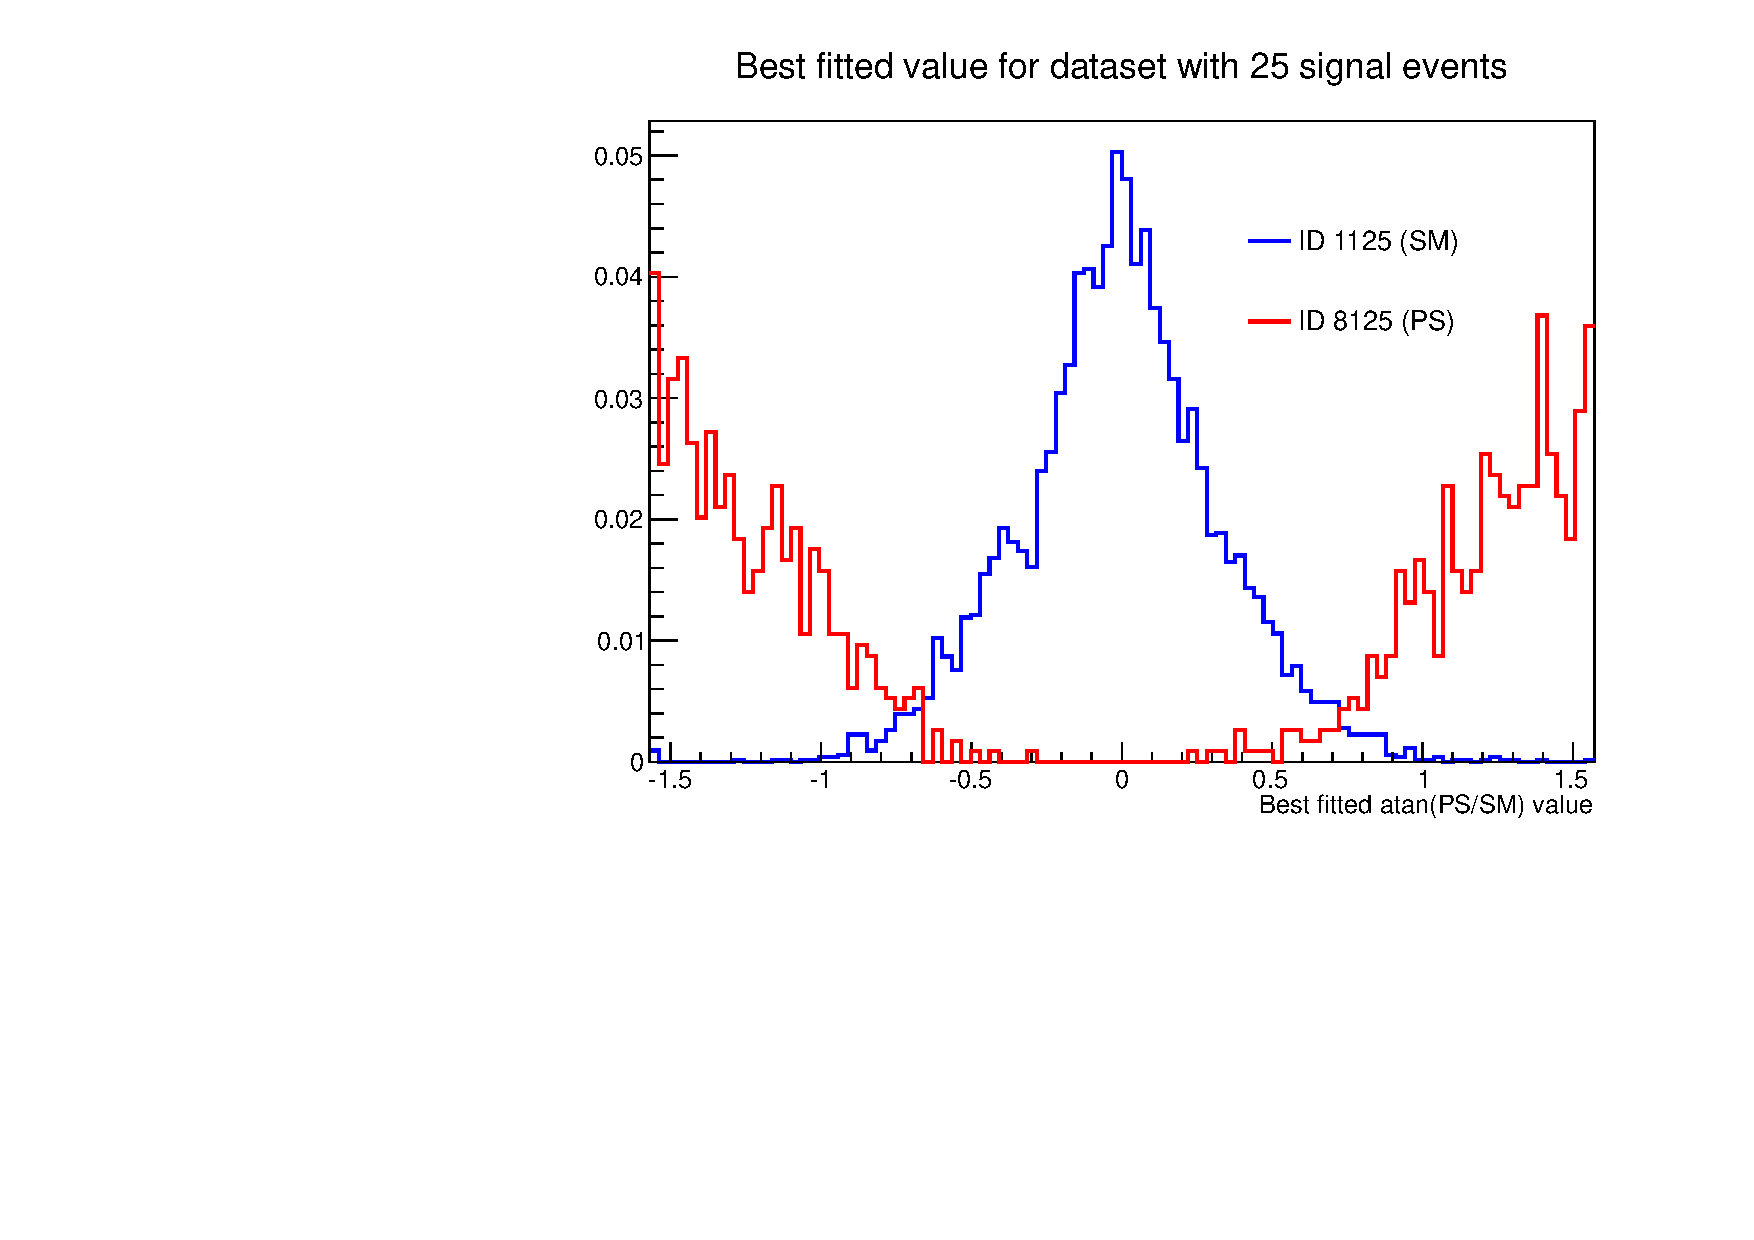
\includegraphics[width=0.48\textwidth]{figures/A1A3Fit_A3ZZA1ZZComparison_25.pdf}
    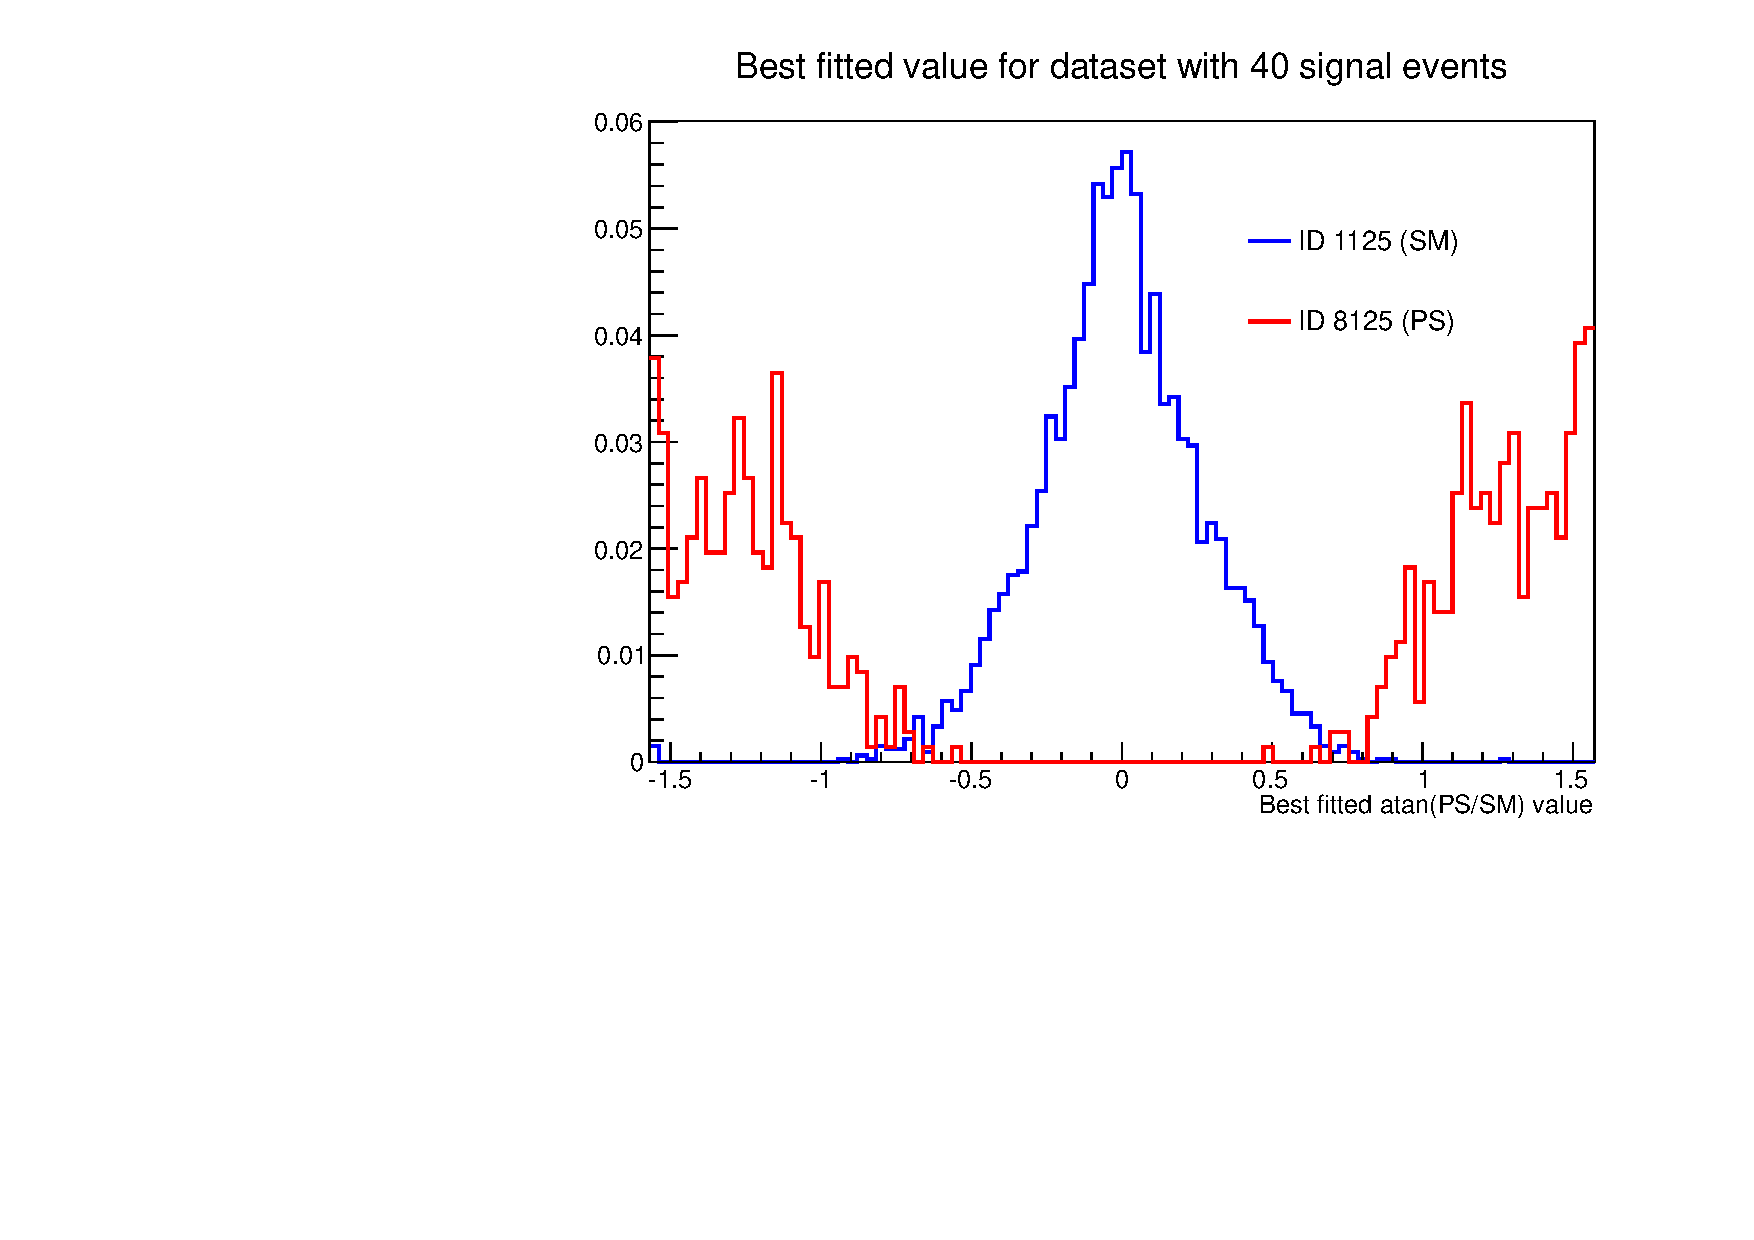
\includegraphics[width=0.48\textwidth]{figures/A1A3Fit_A3ZZA1ZZComparison_40.pdf}
    \caption{Central values of the two-term only, signal-only fits from
    pseudodatasets from MC, for dataset size 25 and 40.}
    \label{fig:A1A3FitCentralValueDistribution}
  \end{center}
\end{figure}

\begin{figure}[htb!]
  \begin{center}
    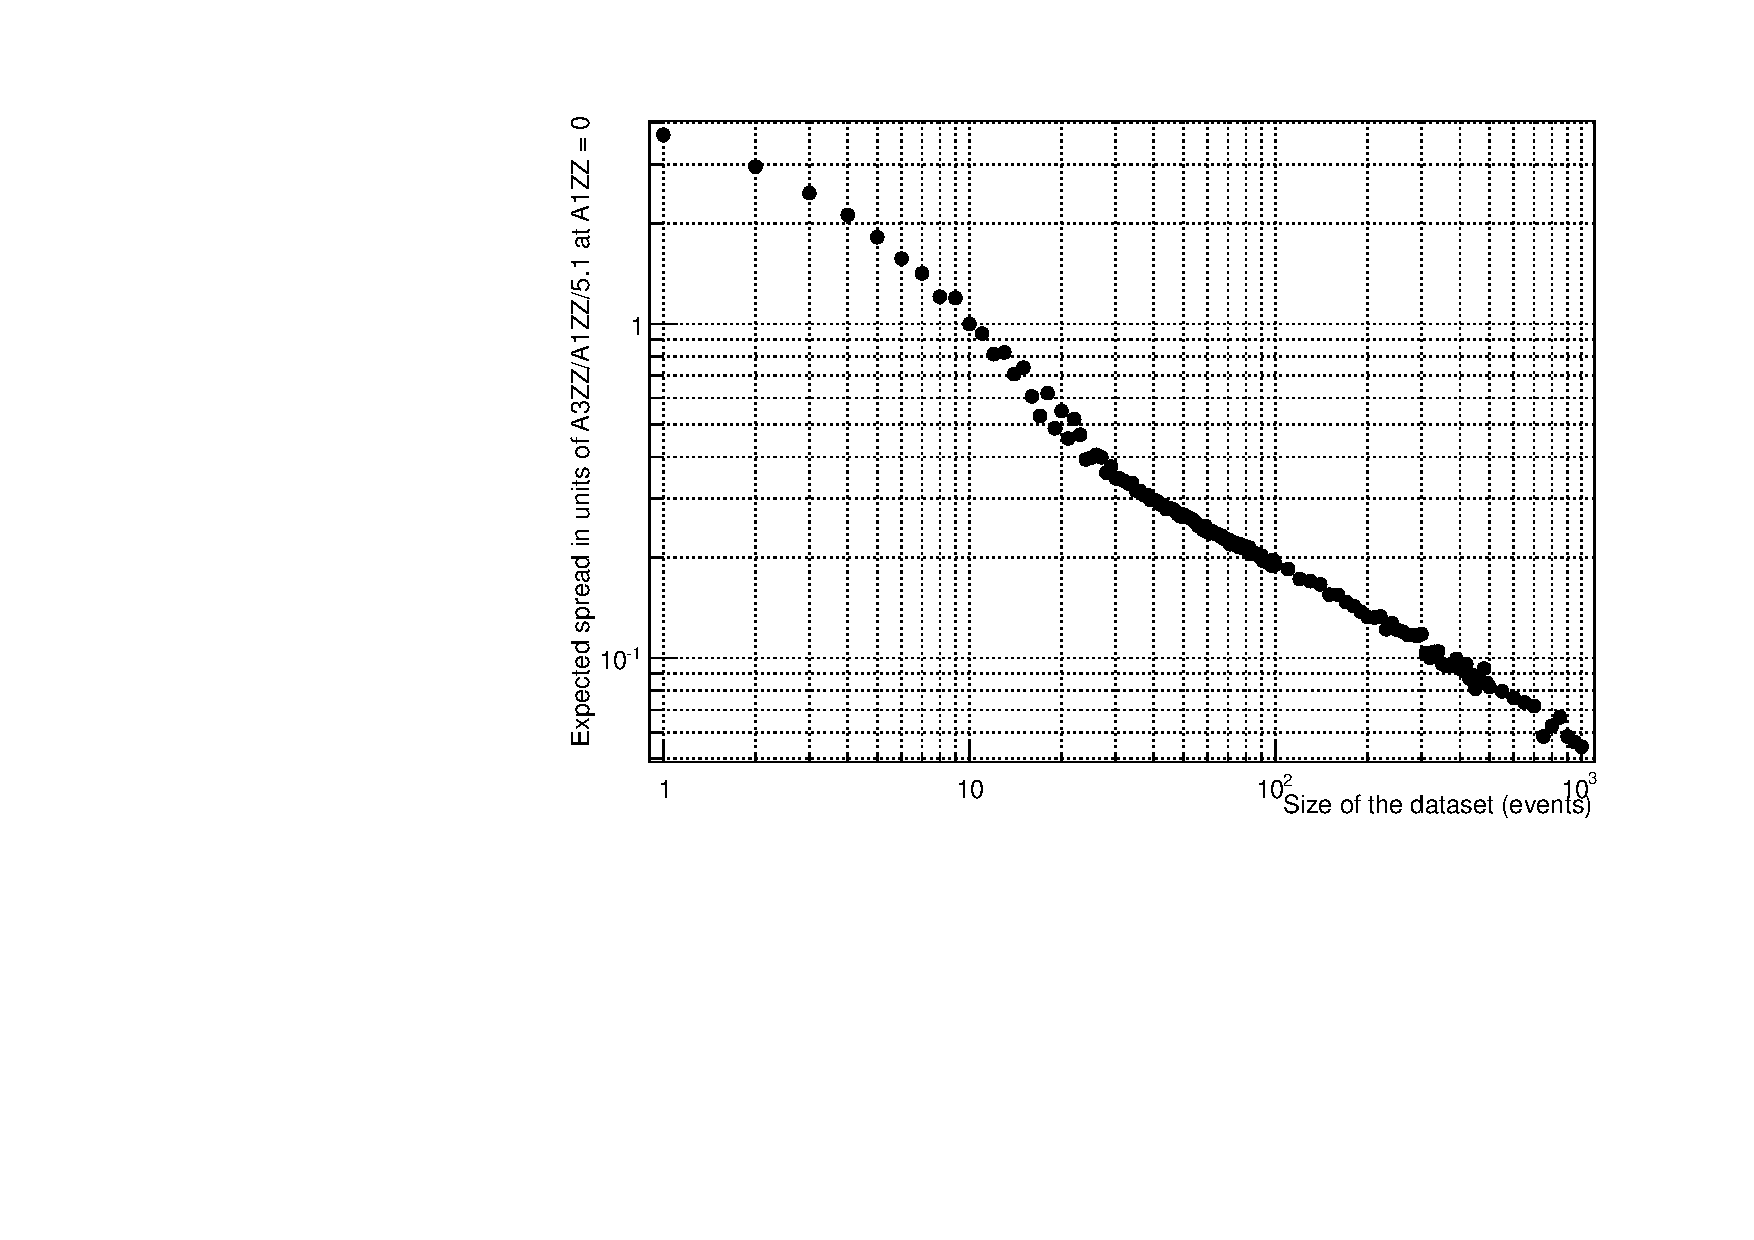
\includegraphics[width=0.48\textwidth]{figures/A1A3Fit_ExpectedSpread.pdf}
    \caption{Spread in units of $A_3^{ZZ}/(5.1 A_1^{ZZ})$ for SM MC as a
    functino of dataset sizes.}
    \label{fig:A1A3FitSpread}
  \end{center}
\end{figure}

\subsubsection{SM-like signal with background fit}
% I call this fit "A1-B fit"

Here I performed fits with only one parameter, $f$, the fraction of background.
Signal model is with only non-zero $A_1^{ZZ}$ term.  An example of the likelihood
profile is shown in figure \ref{fig:A1BFitLikelihoodScan}.  In addition,
to understand if we have any bias or structure in the fitted fraction, fits with
different input number of signal event and background events are repeated few hundred
times for each configuration.  The result is then collected and shown in figure
\ref{fig:A1BFitFractionBias}.  I compared the median fitted background yield (fraction
multiplied by total dataset size) to the true (input) background yield, and plotted
the fractional change.  The red color at 0 means that there is no bias observed,
at least if we take median as the representative, while other colors indicate an
underestimation.  We see that there is a blue valley at the low-background yield
region, which translates into a couple events underestimated.  A slighly more
troublesome region is the orange-ish color everywhere, which is roughly 5-10\%
underestimation.  This both points to the fact that there is some small discrepancy
between generated maps and MC distributions (could be signal or background).
As a quick-and-dirty test, if we manually increase the likelihood of background by
3\% for all events, we can eliminate the bias on the plateau region.

Since this is a toy scenario, there are many things not up-to-speed with what
we will be using in the end.  First of all, the signal model used contains only
$A_1^{ZZ}$ term, while in reality for SM Higgs there will be some small effective
coupling to $\gamma^*$.  Also I didn't separate the maps between electron channels
and muon channels.  All the maps I use here are done with muon smearing and efficiencies.
In addition this is 7D fit, with $E_{CM} = 125$ GeV.  For background events obviously
we need to cut a small window around 125 GeV, and this induces extra uncertainty.
Despite all the caveats, the result turns out reasonable, surprisingly.  Let's move
up one step in fit complexity.


\begin{figure}[htb!]
  \begin{center}
    
\includegraphics[width=0.48\textwidth]{figures/PlaceHolder.pdf}
    \caption{Likelihood scan for SM-like signal + background fit for a pseudo-dataset
    with X signal and Y background events.}
    \label{fig:A1BFitLikelihoodScan}
  \end{center}
\end{figure}

\begin{figure}[htb!]
  \begin{center}
    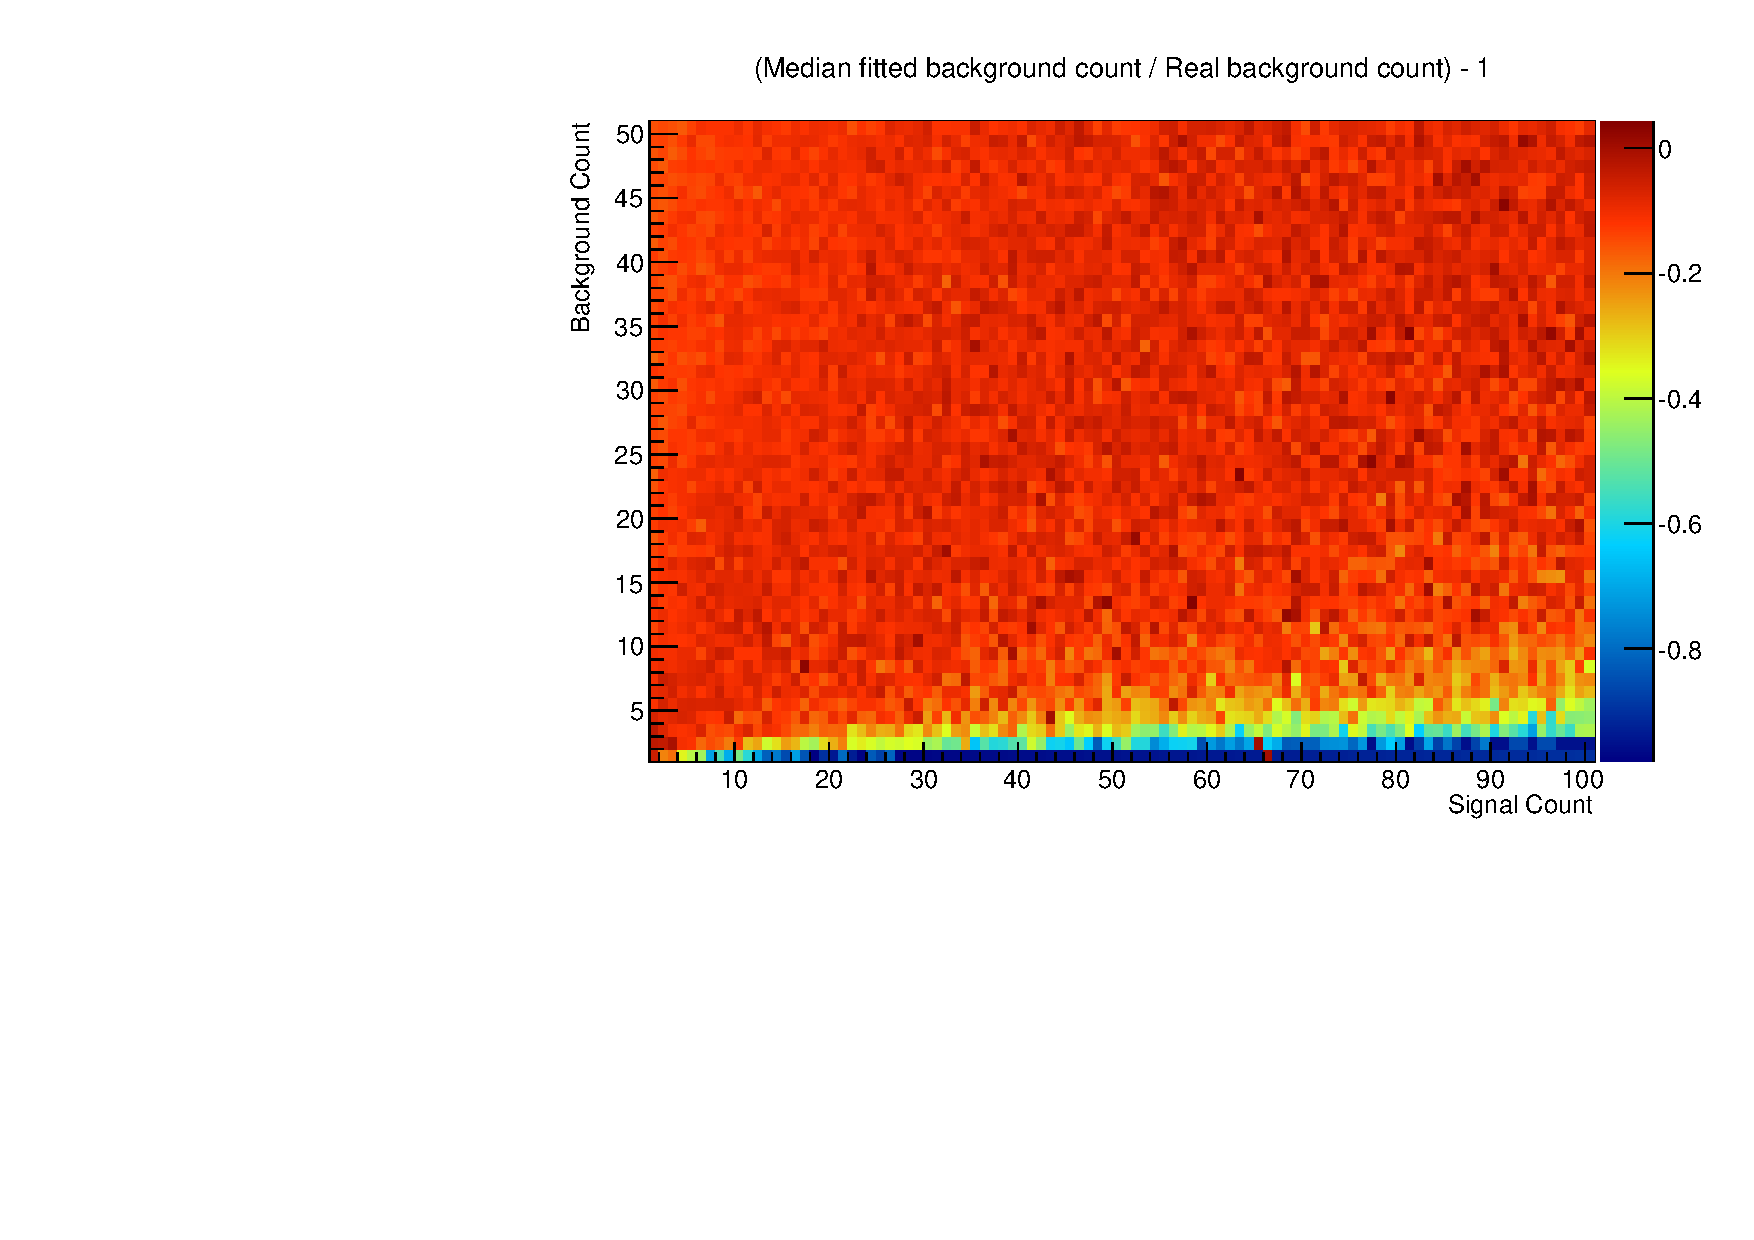
\includegraphics[width=0.48\textwidth]{figures/A1BFit_BackgroundBias.pdf}
    \caption{Bias study for the SM-like signal + background fit for different pseudo-dataset
    sizes}
    \label{fig:A1BFitFractionBias}
  \end{center}
\end{figure}


\subsubsection{SM-like signal with CP-odd term plus background}
% "A1-A3-B" fit

One of the primary goal for this effort is to infer on Lagrangian parameters, we add $A_3^{ZZ}$ back
into the fit.  Similar reason as the previous sections, we only have two free-parameters to fit for:
$A_3^{ZZ} / A_1^{ZZ}$ ratio as well as the background fraction $f$.  An example likelihood scan for
a fit to pseudo-dataset with 40 SM signal events and 10 background events is shown in figure
\ref{fig:A1A3BFitLikelihoodExample}.  The white dot shows where the best fit point is.

I repeated the fit with different signal model (SM Higgs or pseudoscalar) with different signal-to-background
yield configurations.  Collection of the central values is shown in figure \ref{fig:A1A3BFitCentralValueDistribution}.
The presense of background widens distribution of fitted $A_3^{ZZ} / A_1^{ZZ}$ distributions, but
we can still maintain good separation power.

The picture on bias on background yield remains.  We see an overall 5-10\% underestimation of background
everywhere, and a couple events underestimation when signal is overwhelmingly large compared to background.
In terms of impact on signal, a more appropriate quantity to look at is the overestimation of signal
divided by the amount of input signals.  The plots are shown in figure \ref{fig:A1A3BFitBackgroundBias}.
Different contours of iso-overestimation are drawn.  When signal and background are compatible, the
overestimation is about 10\%.  However, as stated before, this is just a toy scenario study, and
the final maps will be updated with better detector resolution modeling etc., and we expect the reality to
be better than this.

Expected spread of $A_3^{ZZ} / A_1^{ZZ}$ in the presense of background is also redone, as shown in figure
\ref{fig:A1A3BFitSignalSpread}.

\begin{figure}[htb!]
  \begin{center}
    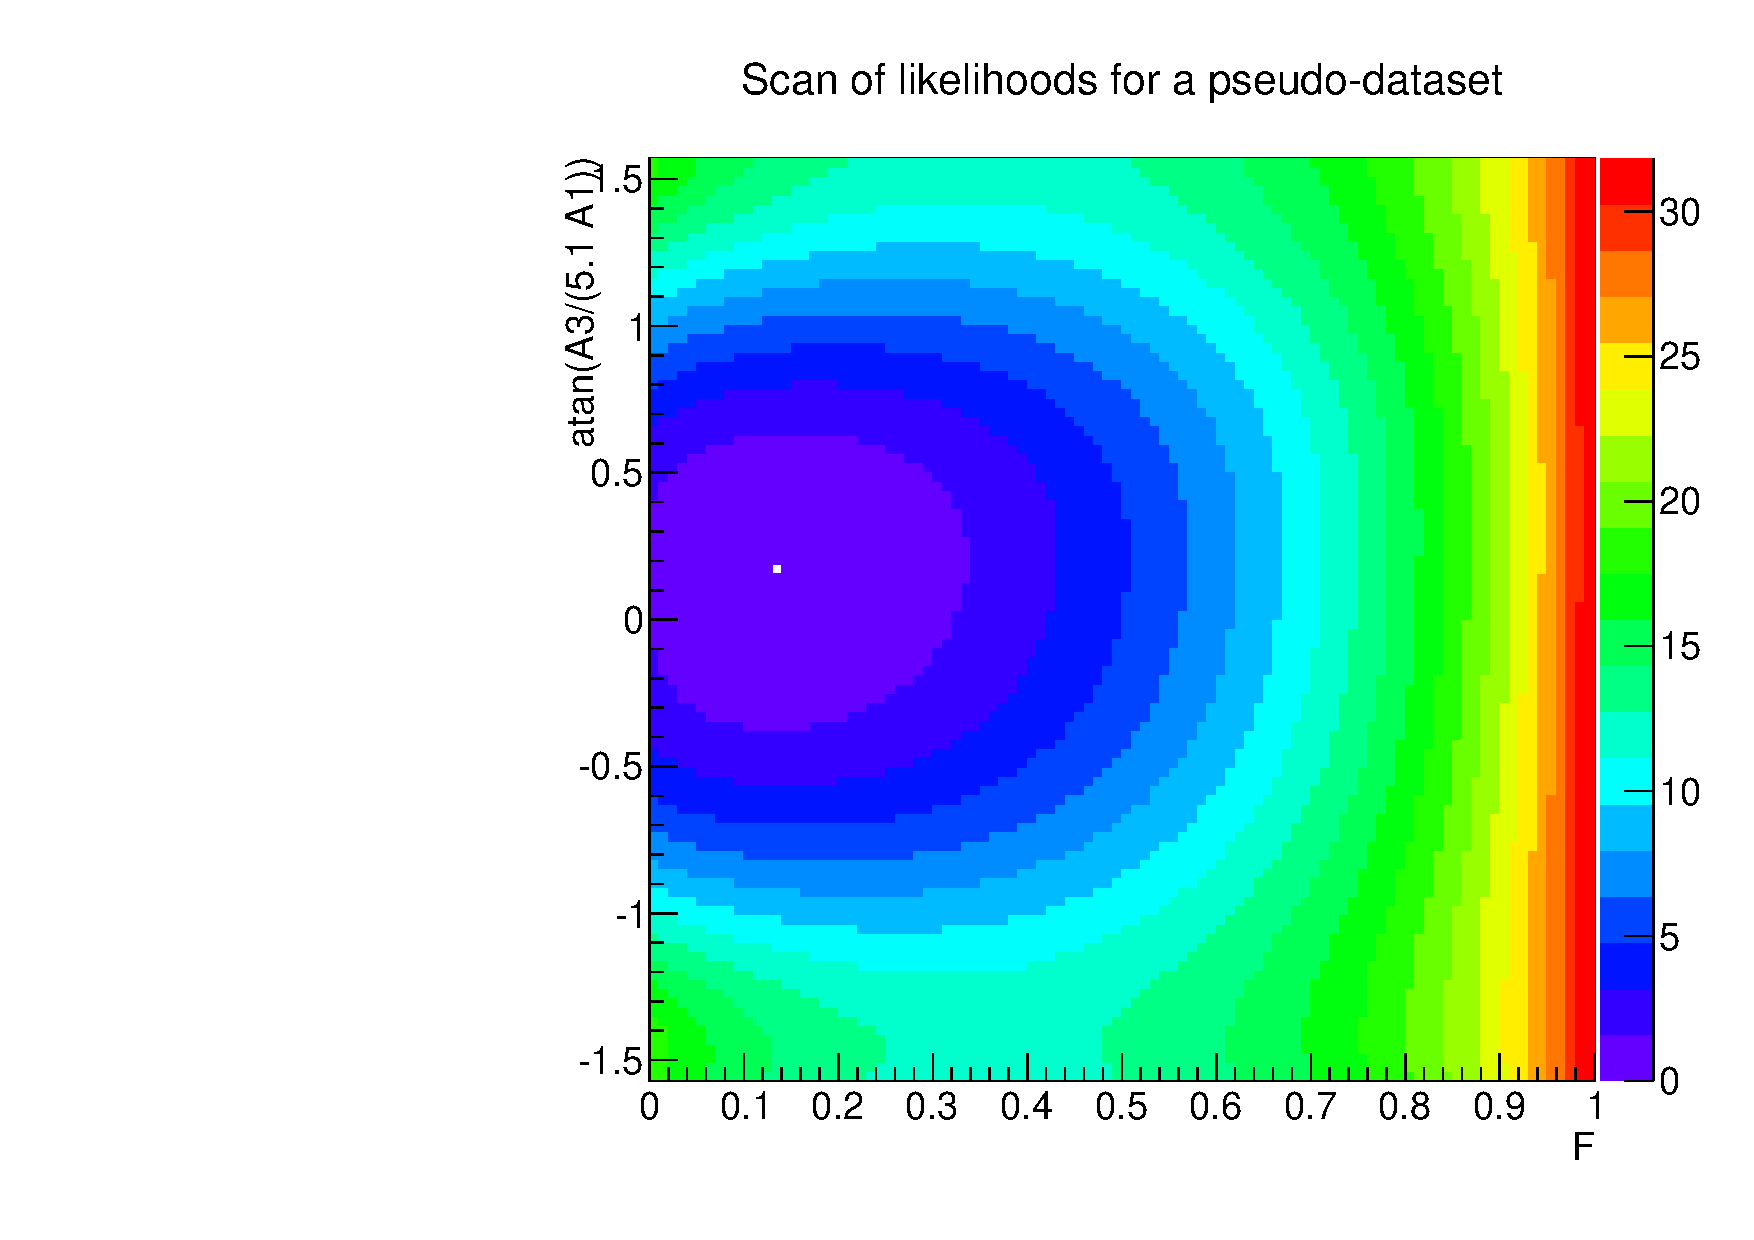
\includegraphics[width=0.48\textwidth]{figures/A1A3BFit_ScanLikelihood_40_10_10.pdf}
    \caption{Example likelihood for the 2D fit.}
    \label{fig:A1A3BFitLikelihoodExample}
  \end{center}
\end{figure}

\begin{figure}[htb!]
  \begin{center}
    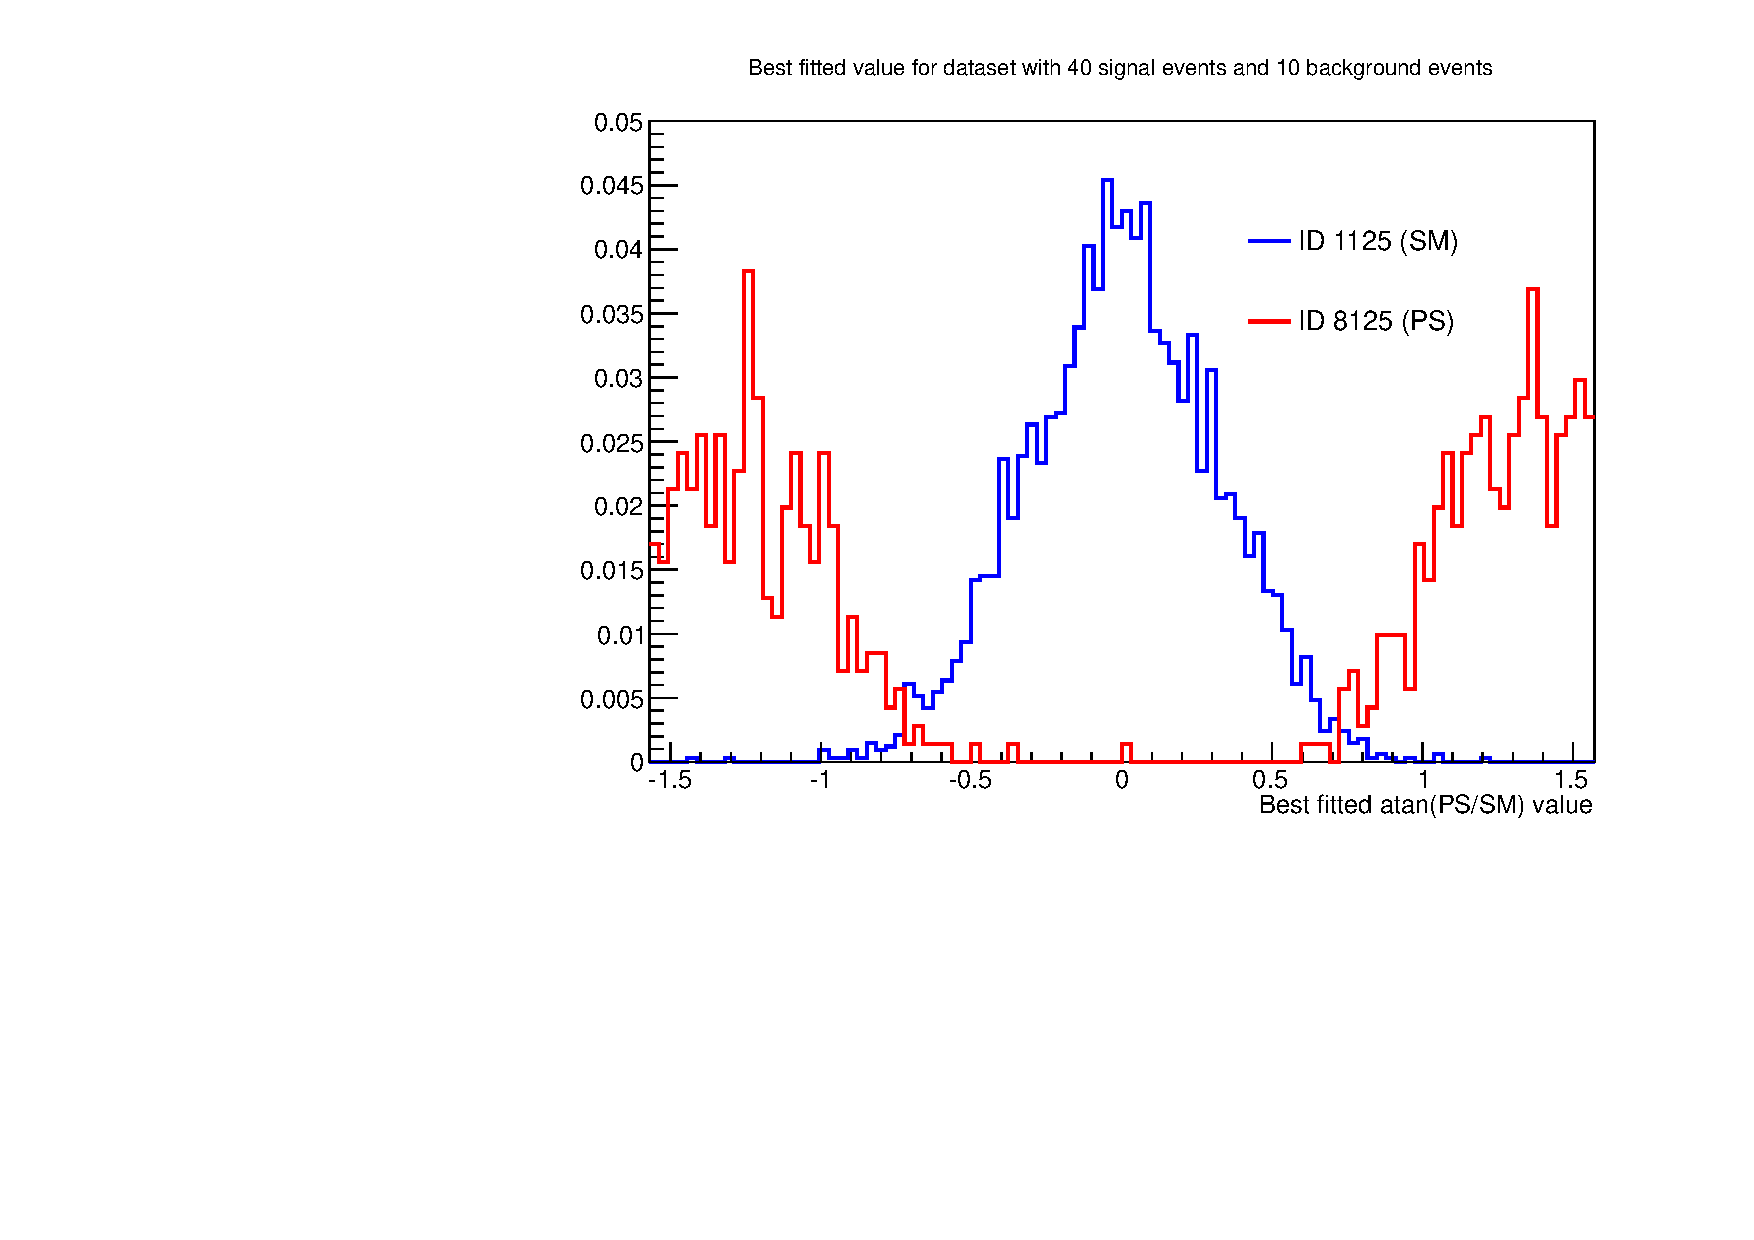
\includegraphics[width=0.48\textwidth]{figures/A1A3BFit_Comparison_40_10.pdf}
    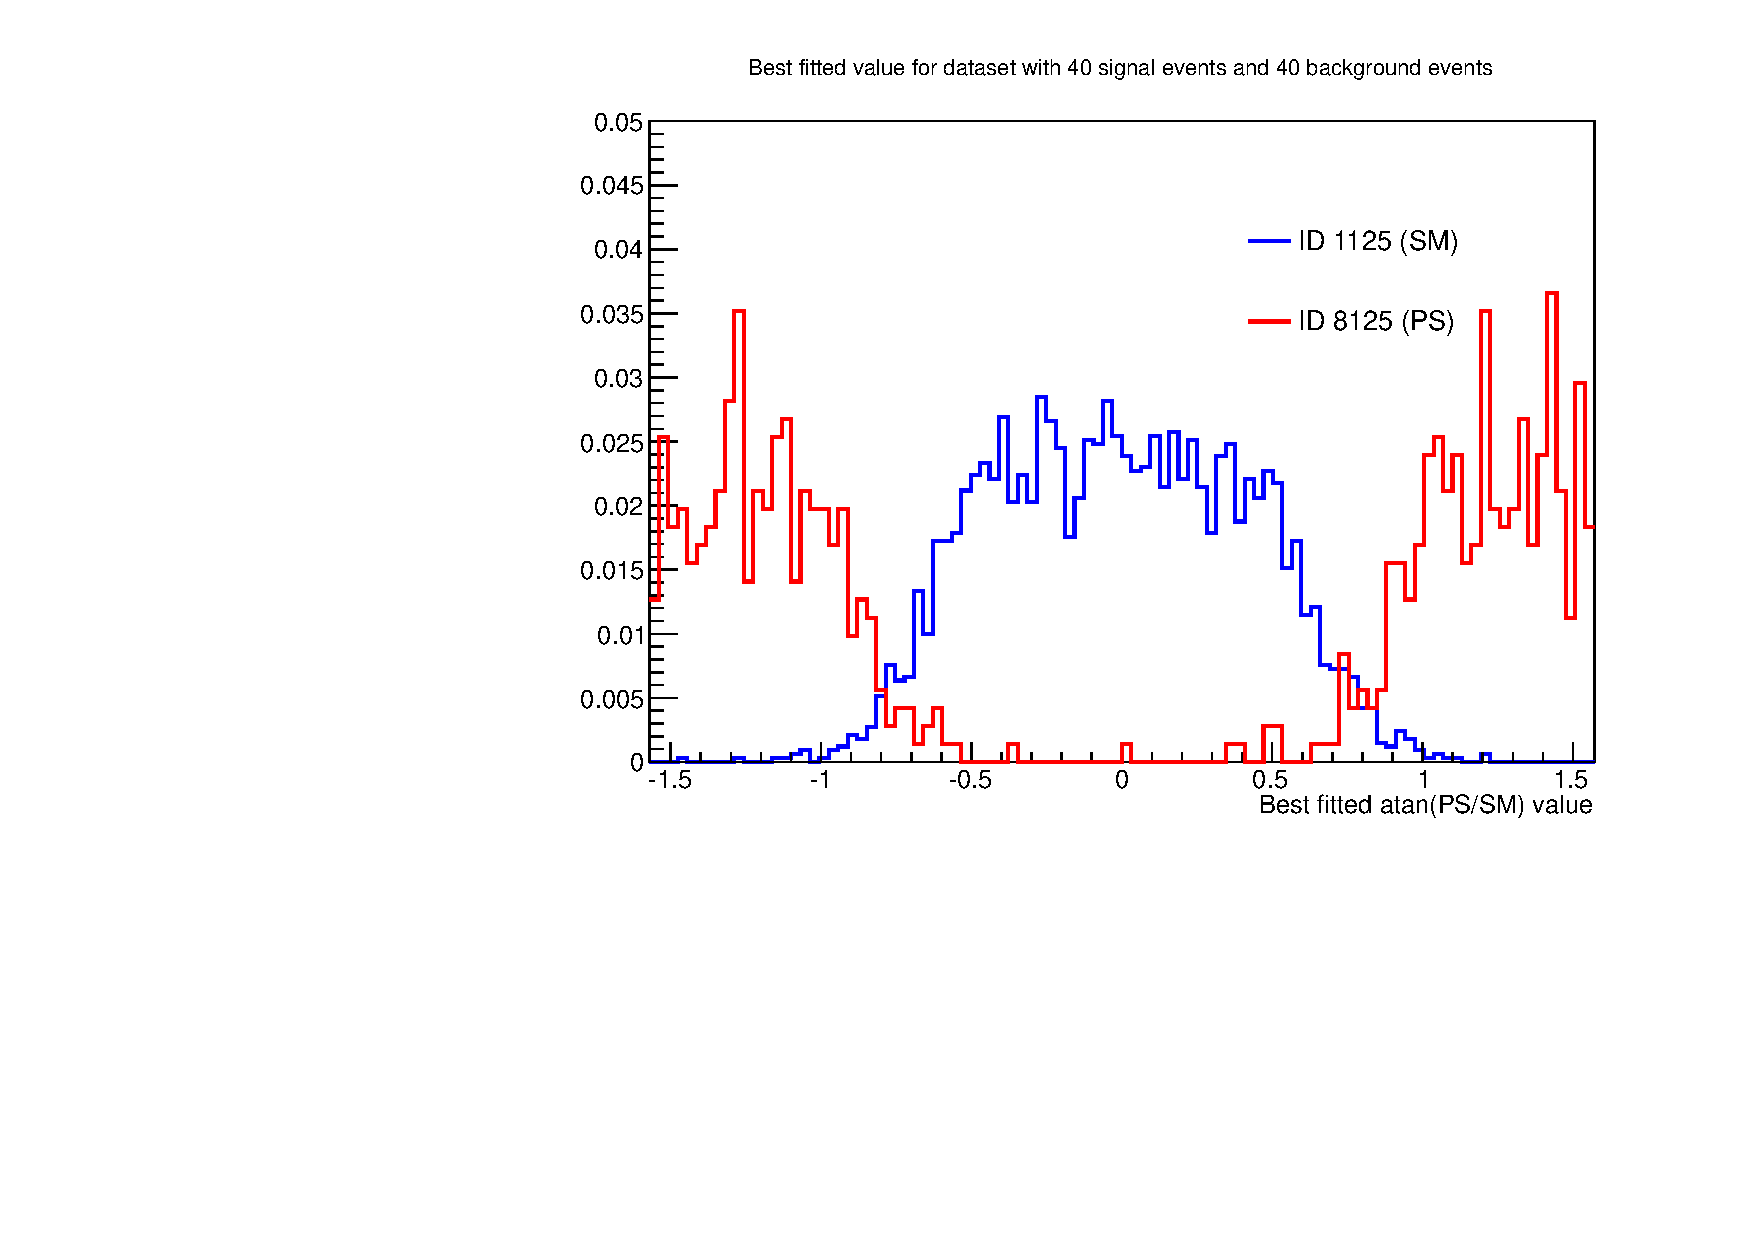
\includegraphics[width=0.48\textwidth]{figures/A1A3BFit_Comparison_40_40.pdf}
    \caption{Central values of the two-parameter fits from
    pseudodatasets from MC, for dataset size 40+10 and 40+40.}
    \label{fig:A1A3BFitCentralValueDistribution}
  \end{center}
\end{figure}

\begin{figure}[htb!]
  \begin{center}
    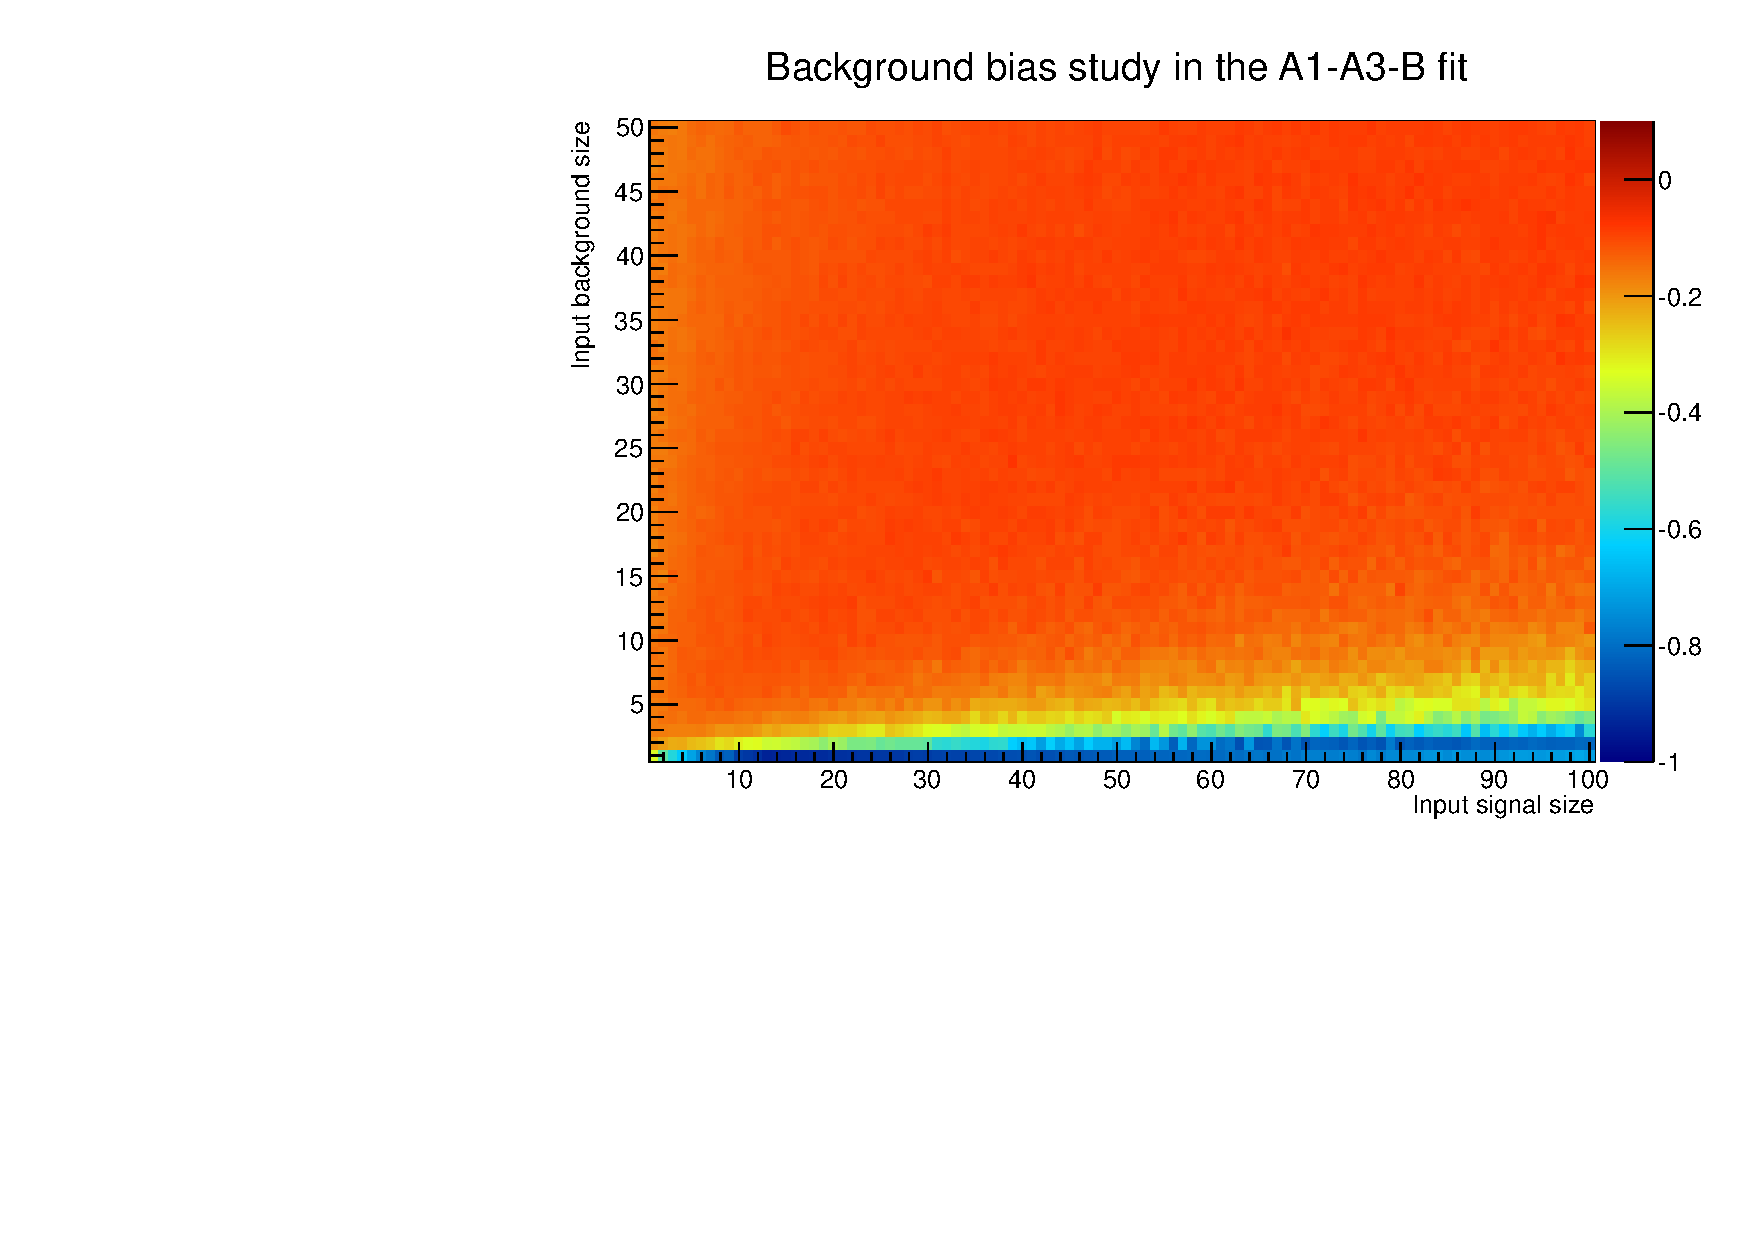
\includegraphics[width=0.48\textwidth]{figures/A1A3BFit_BackgroundBias.pdf}
    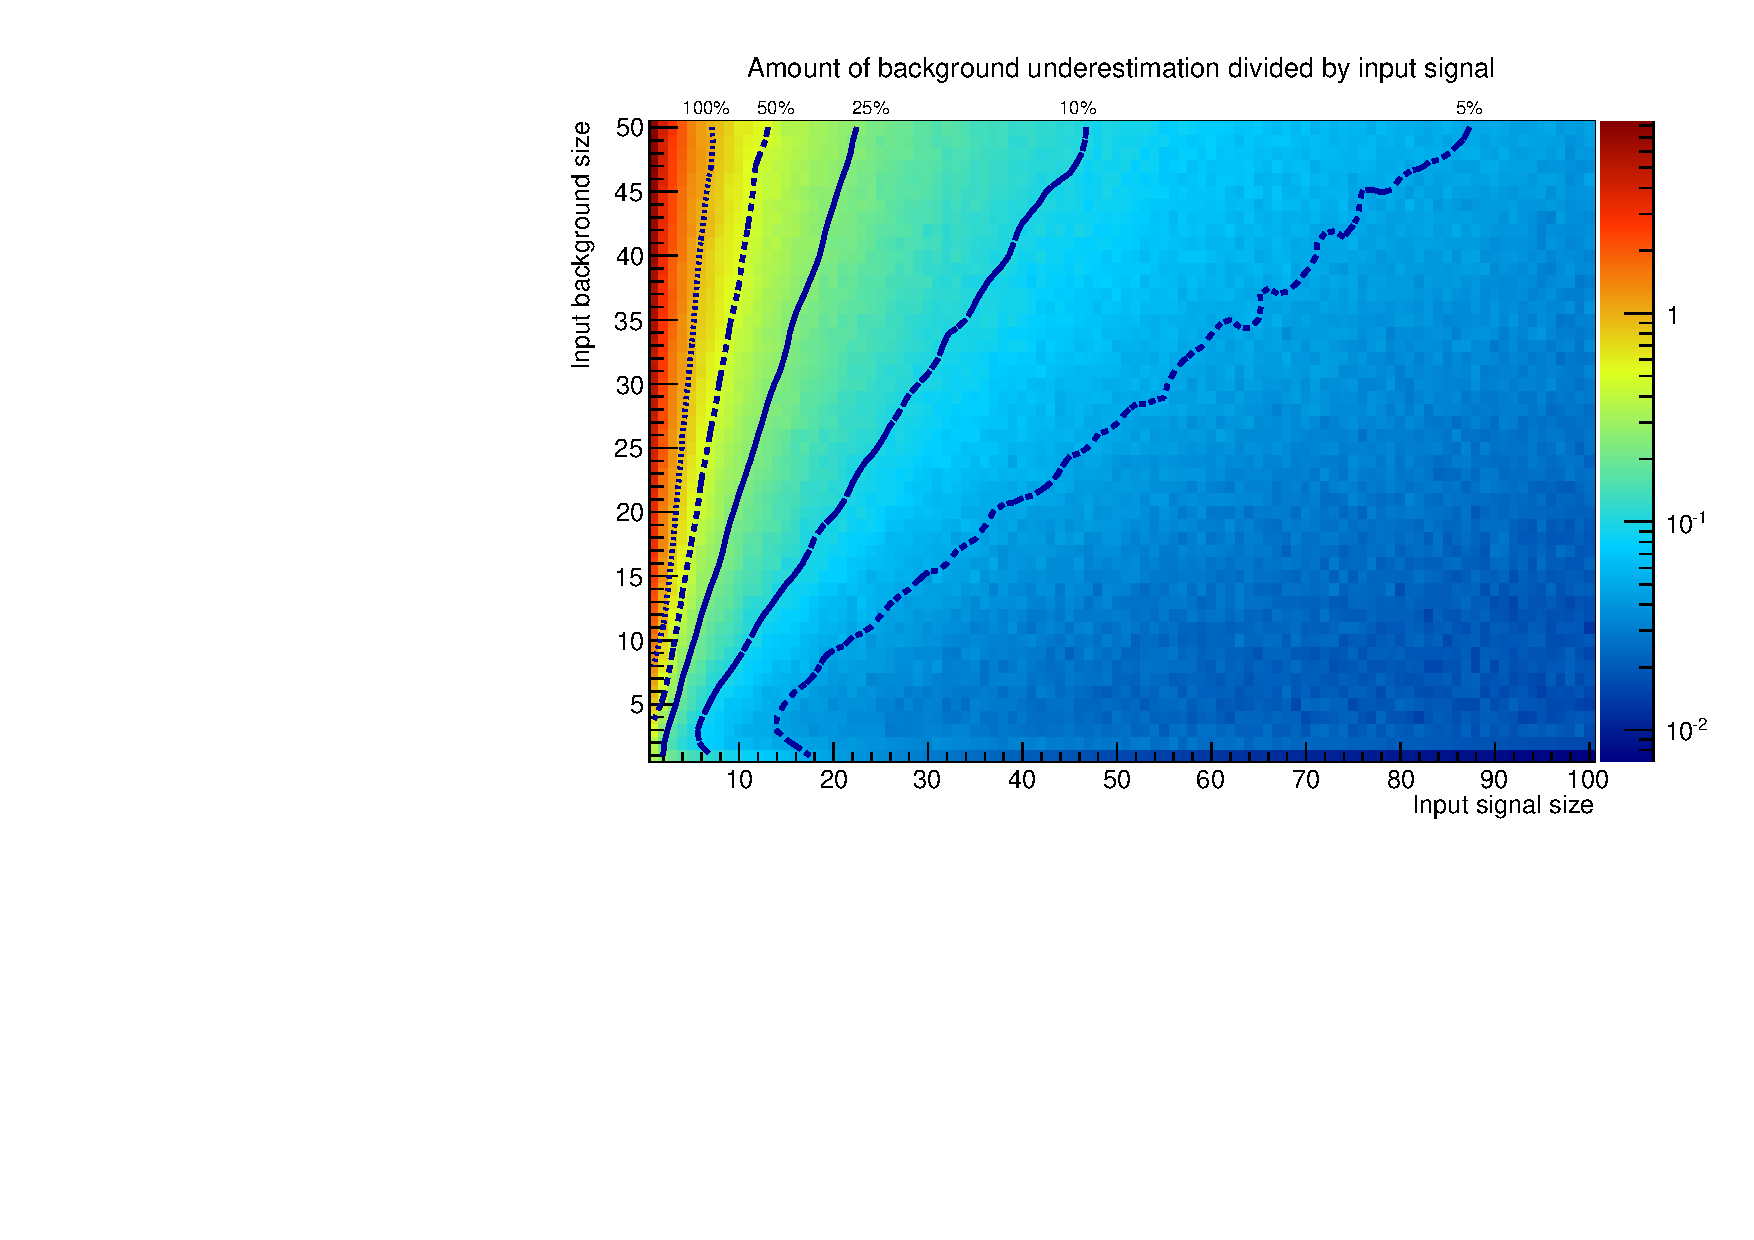
\includegraphics[width=0.48\textwidth]{figures/A1A3BFit_Underestimation.pdf}
    \caption{Background bias study for the 2D fit.  Upper plot shows the underestimation of background
    in units of input background count, and the lower plot is in units of input signal count.  Lines
    are the iso-underestimation contours.}
    \label{fig:A1A3BFitBackgroundBias}
  \end{center}
\end{figure}

\begin{figure}[htb!]
  \begin{center}
    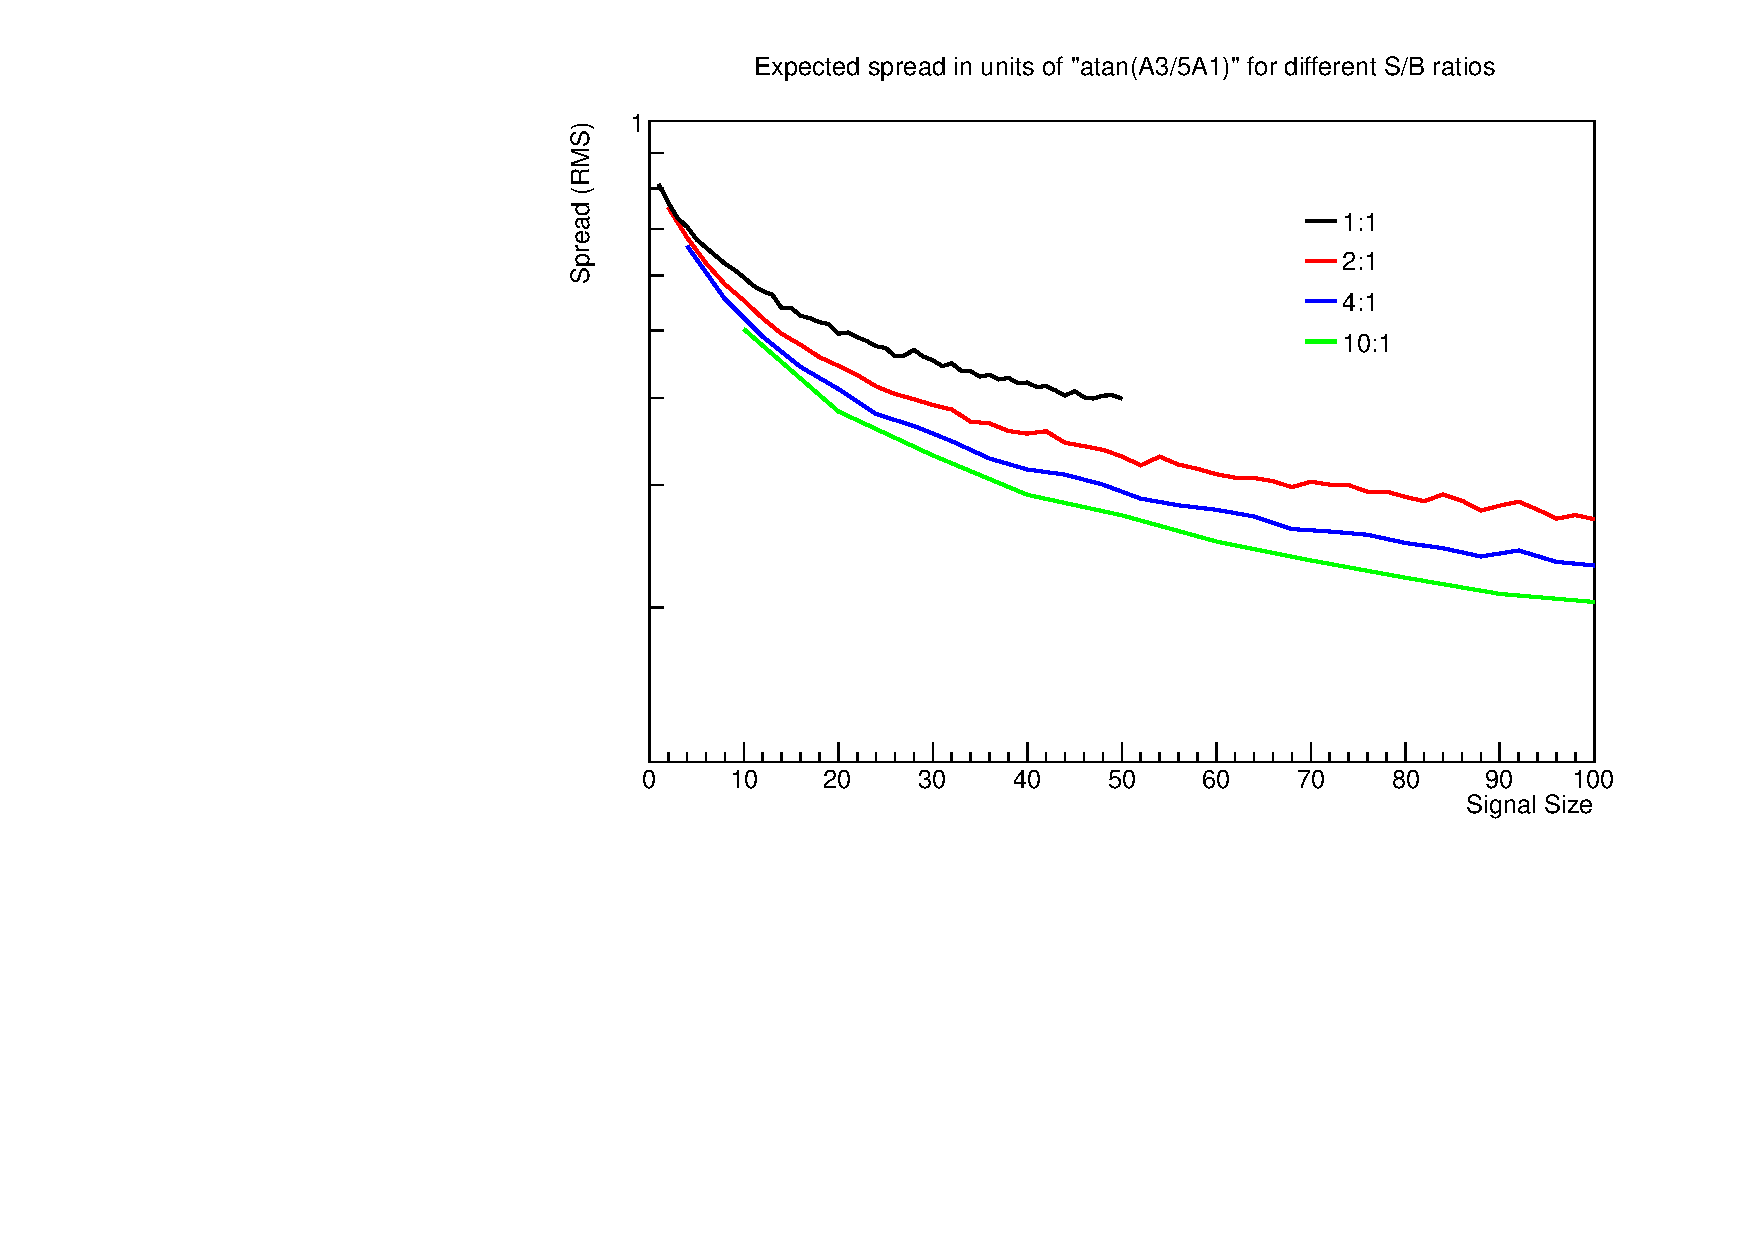
\includegraphics[width=0.48\textwidth]{figures/A1A3BFit_SignalSpread.pdf}
    \caption{Expected fitted signal spread (in units of $atan(A3/(5 A1))$) for different S:B ratios.}
    \label{fig:A1A3BFitSignalSpread}
  \end{center}
\end{figure}


\subsubsection{Signal-only fit with a single nuisance parameter}
% A1-A3-N Fit

Since in reality we have systematics which will take the form of nuisance parameters, let's investigate
how things look in the presense of a single nuisance parameter.  As usual, I start with the simpliest
case.  I tried out a fit for $A_3^{ZZ}/A_1^{ZZ}$ ratio as well as a nuisance parameter for the lepton
energy scale.  The alternate maps are generated with a shift in energy by $1 \sigma$, where the $\sigma$
is the core of the double-sided crystal ball shape in the lepton resolution modeling.
The treatment of the nuisanse parameter in the fit is described in previous sections.

We can scan through all parameters and plot the likelihood profile, shown in figure
\ref{fig:A1A3NFitLikelihoodExample}.  On the y axis the unit is in sigmas of nuisance parameters.
The expected spread in fitted value is plotted as a function of dataset size, figure
\ref{fig:A1A3NFitExpectedSpread}, and compared
with the case when we do not have nuisance parameters.  We don't see a big
effect from this systematics.  With the dataset size is small, we observe some increase
in RMS of fitted value.  The spread in nuisance parameter scales nicely
as a function of $\sqrt{\text{Dataset size}}$.


\begin{figure}[htb!]
  \begin{center}
    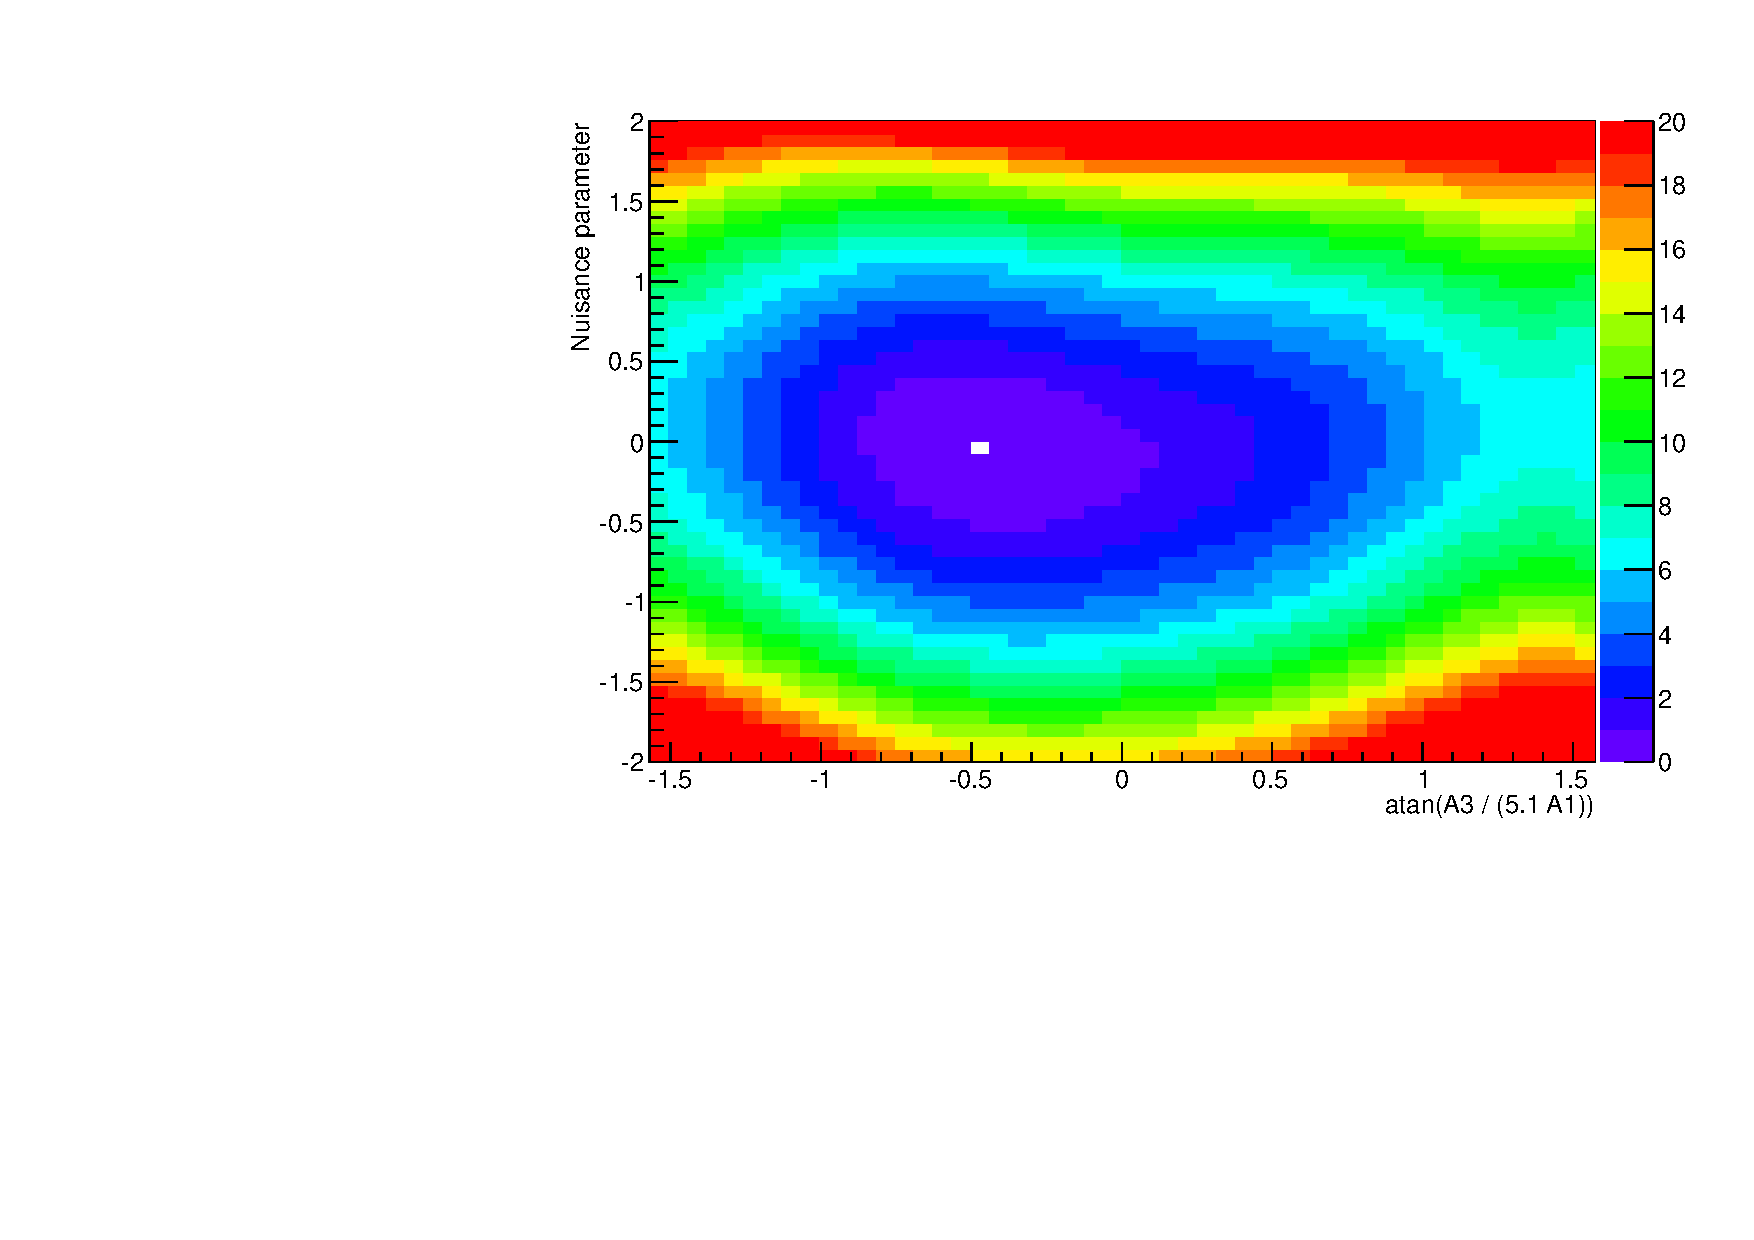
\includegraphics[width=0.48\textwidth]{figures/A1A3NFit_LikelihoodExample_8.pdf}
    \caption{Example likelihood for the signal-only fit with one nuisance parameter of a pseudo-dataset
    consists of 30 SM Higgs signal.}
    \label{fig:A1A3NFitLikelihoodExample}
  \end{center}
\end{figure}

\begin{figure}[htb!]
  \begin{center}
    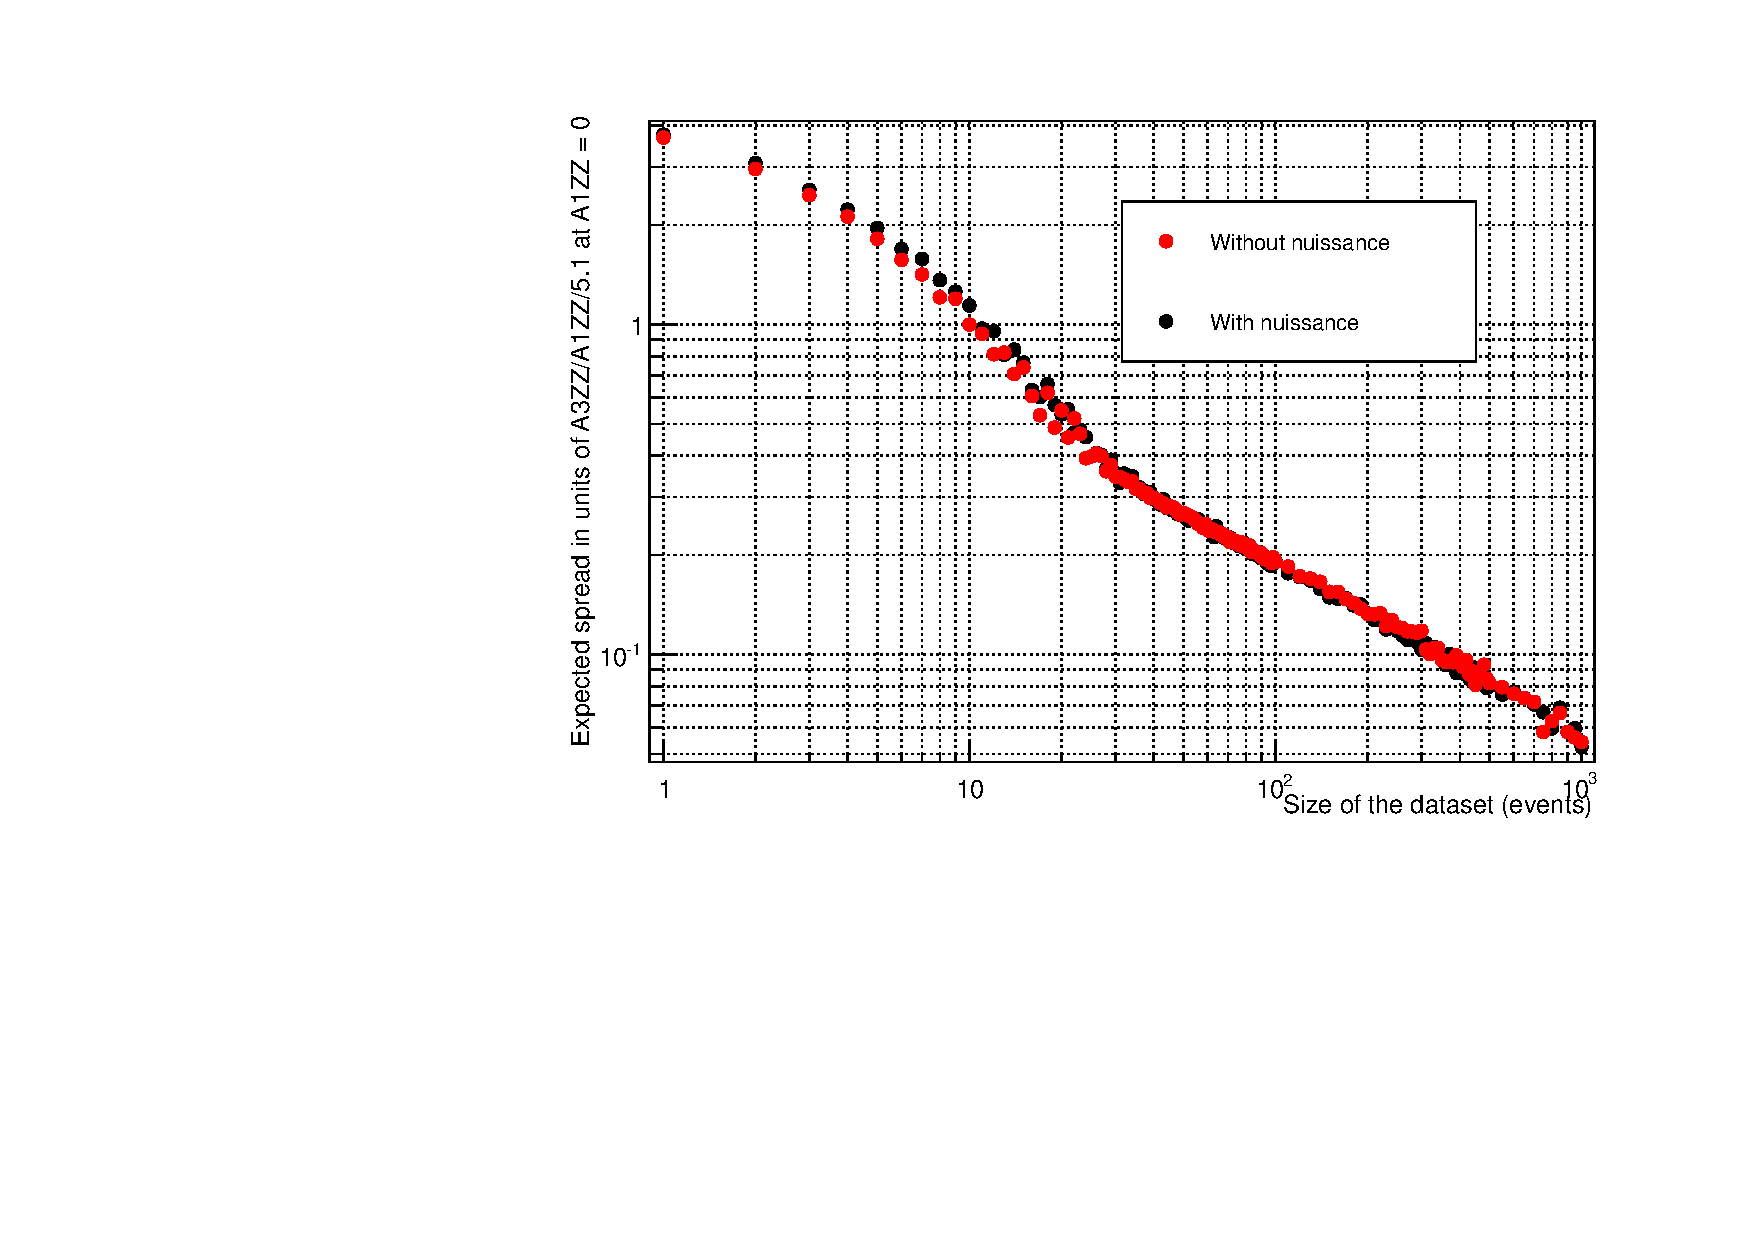
\includegraphics[width=0.48\textwidth]{figures/A1A3NFit_ComparisonOfExpectedSpread.pdf}
    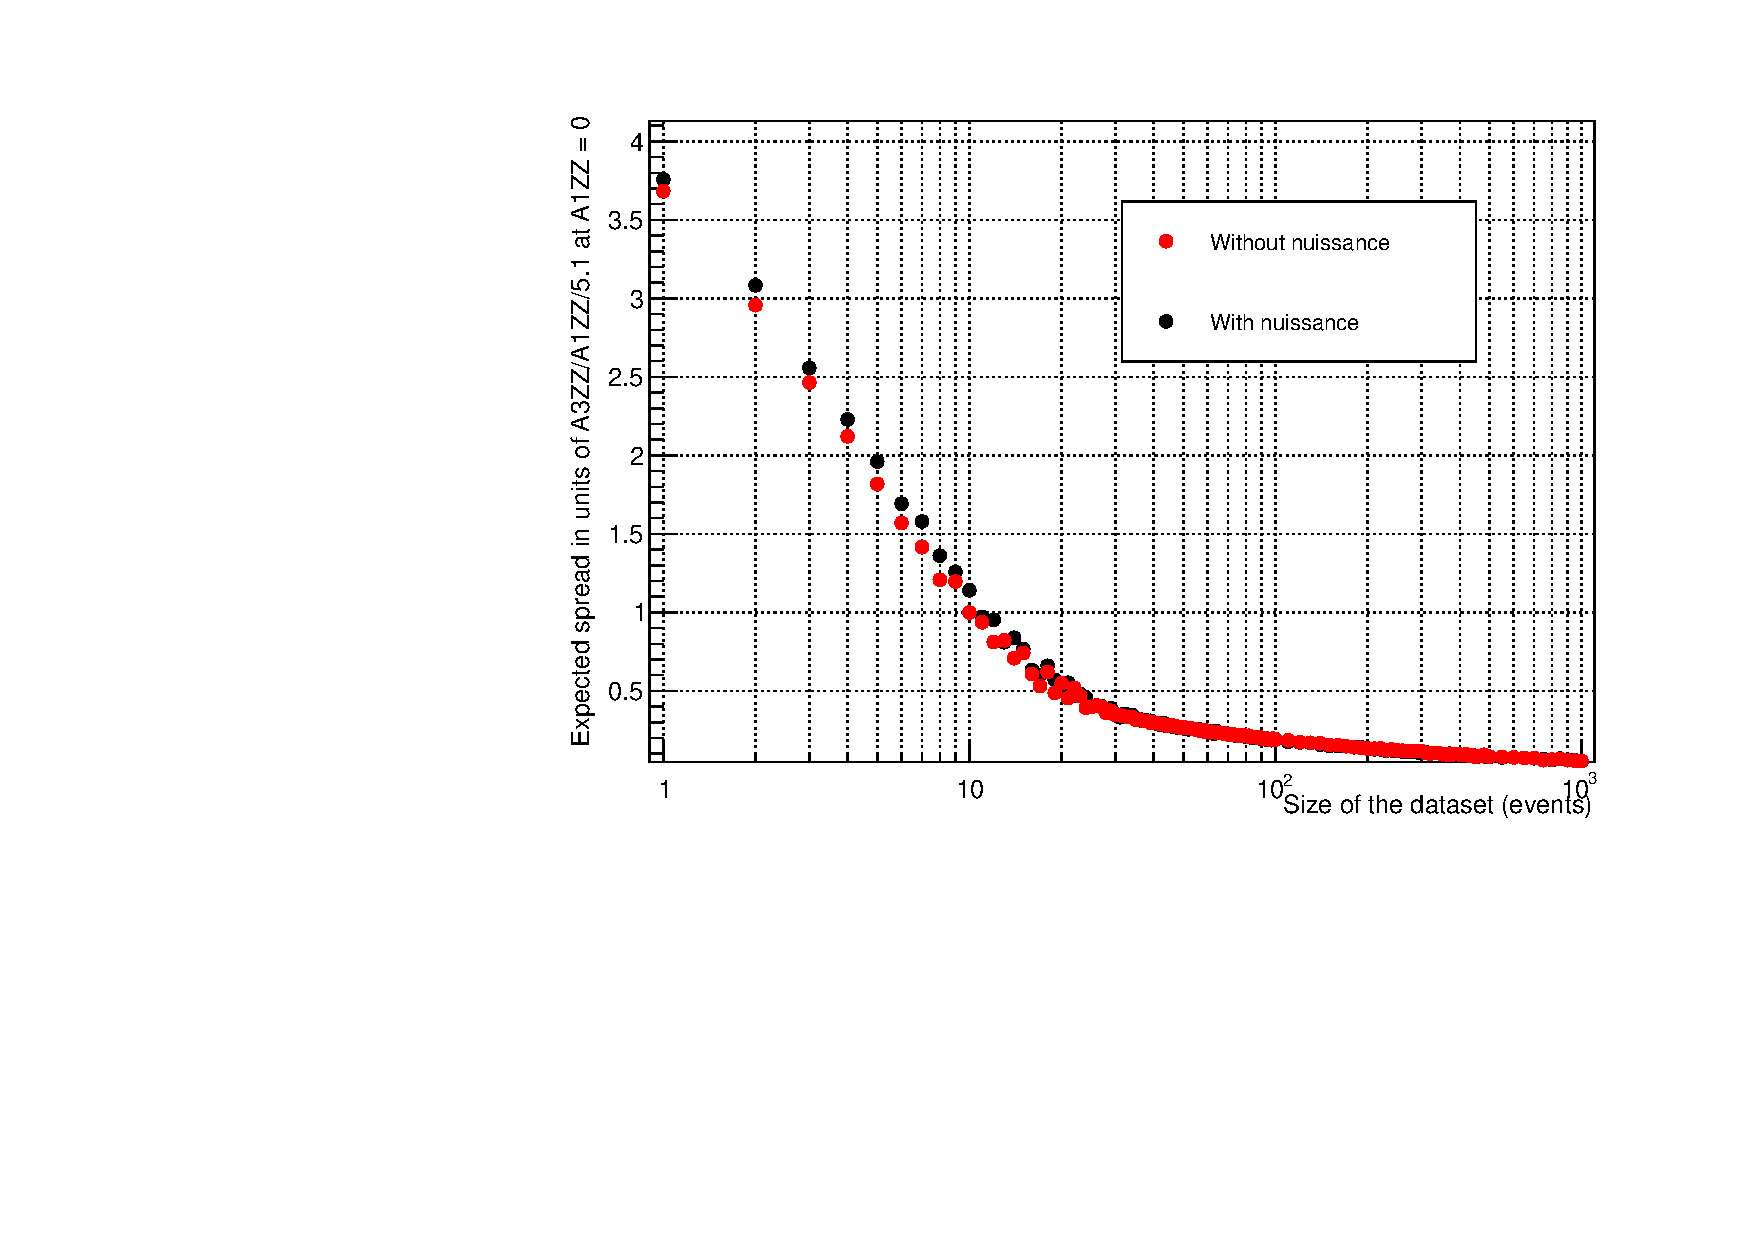
\includegraphics[width=0.48\textwidth]{figures/A1A3NFit_ComparisonOfExpectedSpread_YNormal.pdf}
    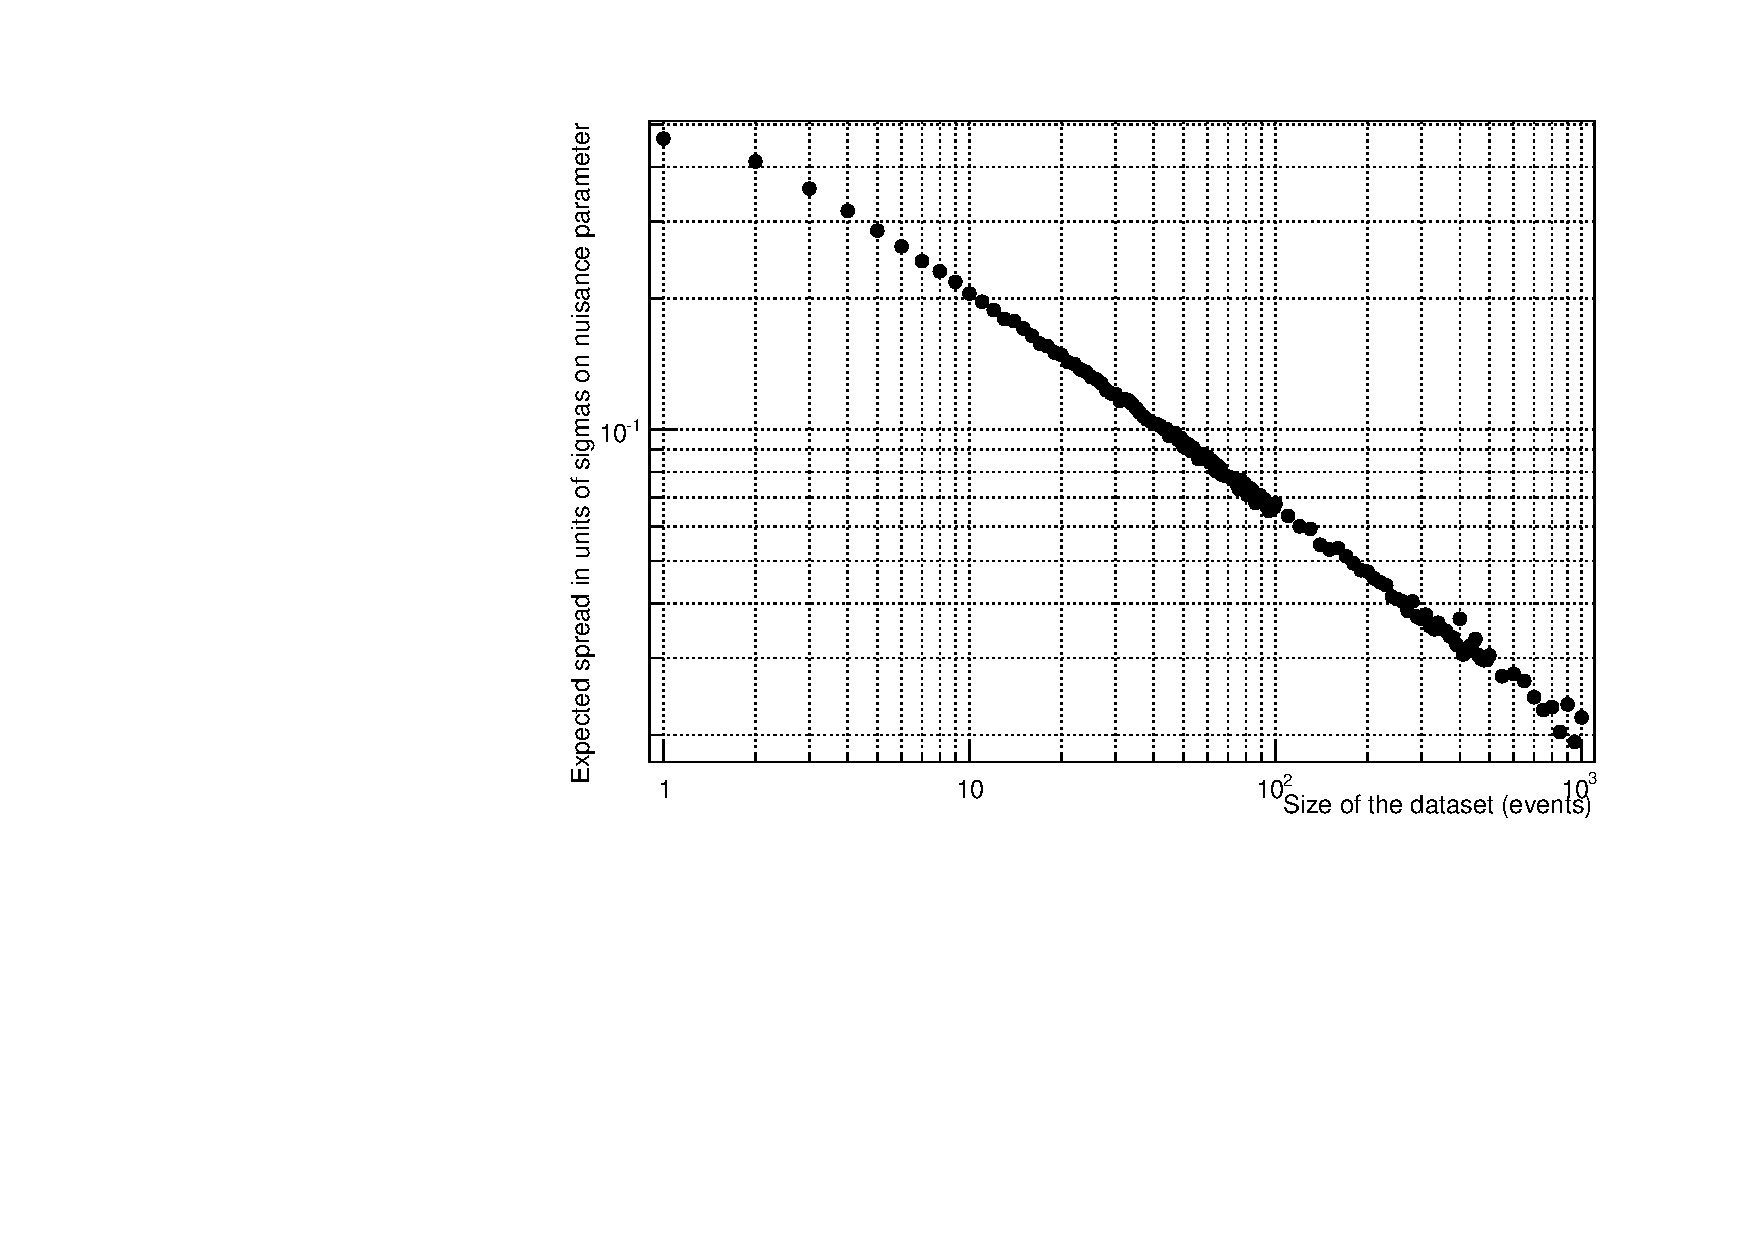
\includegraphics[width=0.48\textwidth]{figures/A1A3NFit_ExpectedSpreadN.pdf}
    \caption{Spread of the fitted central value for $A_3^{ZZ}/(5.1 A_1^{ZZ})$ as well as the nuisance
    parameter.  First two plots are the same except for the y-axis scale.}
    \label{fig:A1A3NFitExpectedSpread}
  \end{center}
\end{figure}

\subsubsection{Signal (including CP-odd term) with background fit with a single nuisance parameter}
% A1-A3-B-N Fit

Here I fit for $A_3^{ZZ}/A_1^{ZZ}$, background fraction while minimizing the nuisance parameter, which
in this case is the same one as in the last sub-sub-section: width on the lepton resolution model.

The fit is still running so I don't know how it will turn out.  Fingers crossed.  One example fit
is shown in figure \ref{fig:A1A3BNFitLikelihoodExample}, where we scan the likelihood across
$atan(A_3^{ZZ}/(5.1\,A_1^{ZZ}))$-Fraction plane, and at every point minimize position for
nuisance parameter.  The best position for nuisance parameter in shown in the right-hand-side figure.

Now let's wait for the repeated fits, which will take a while...


\begin{figure}[htb!]
  \begin{center}
    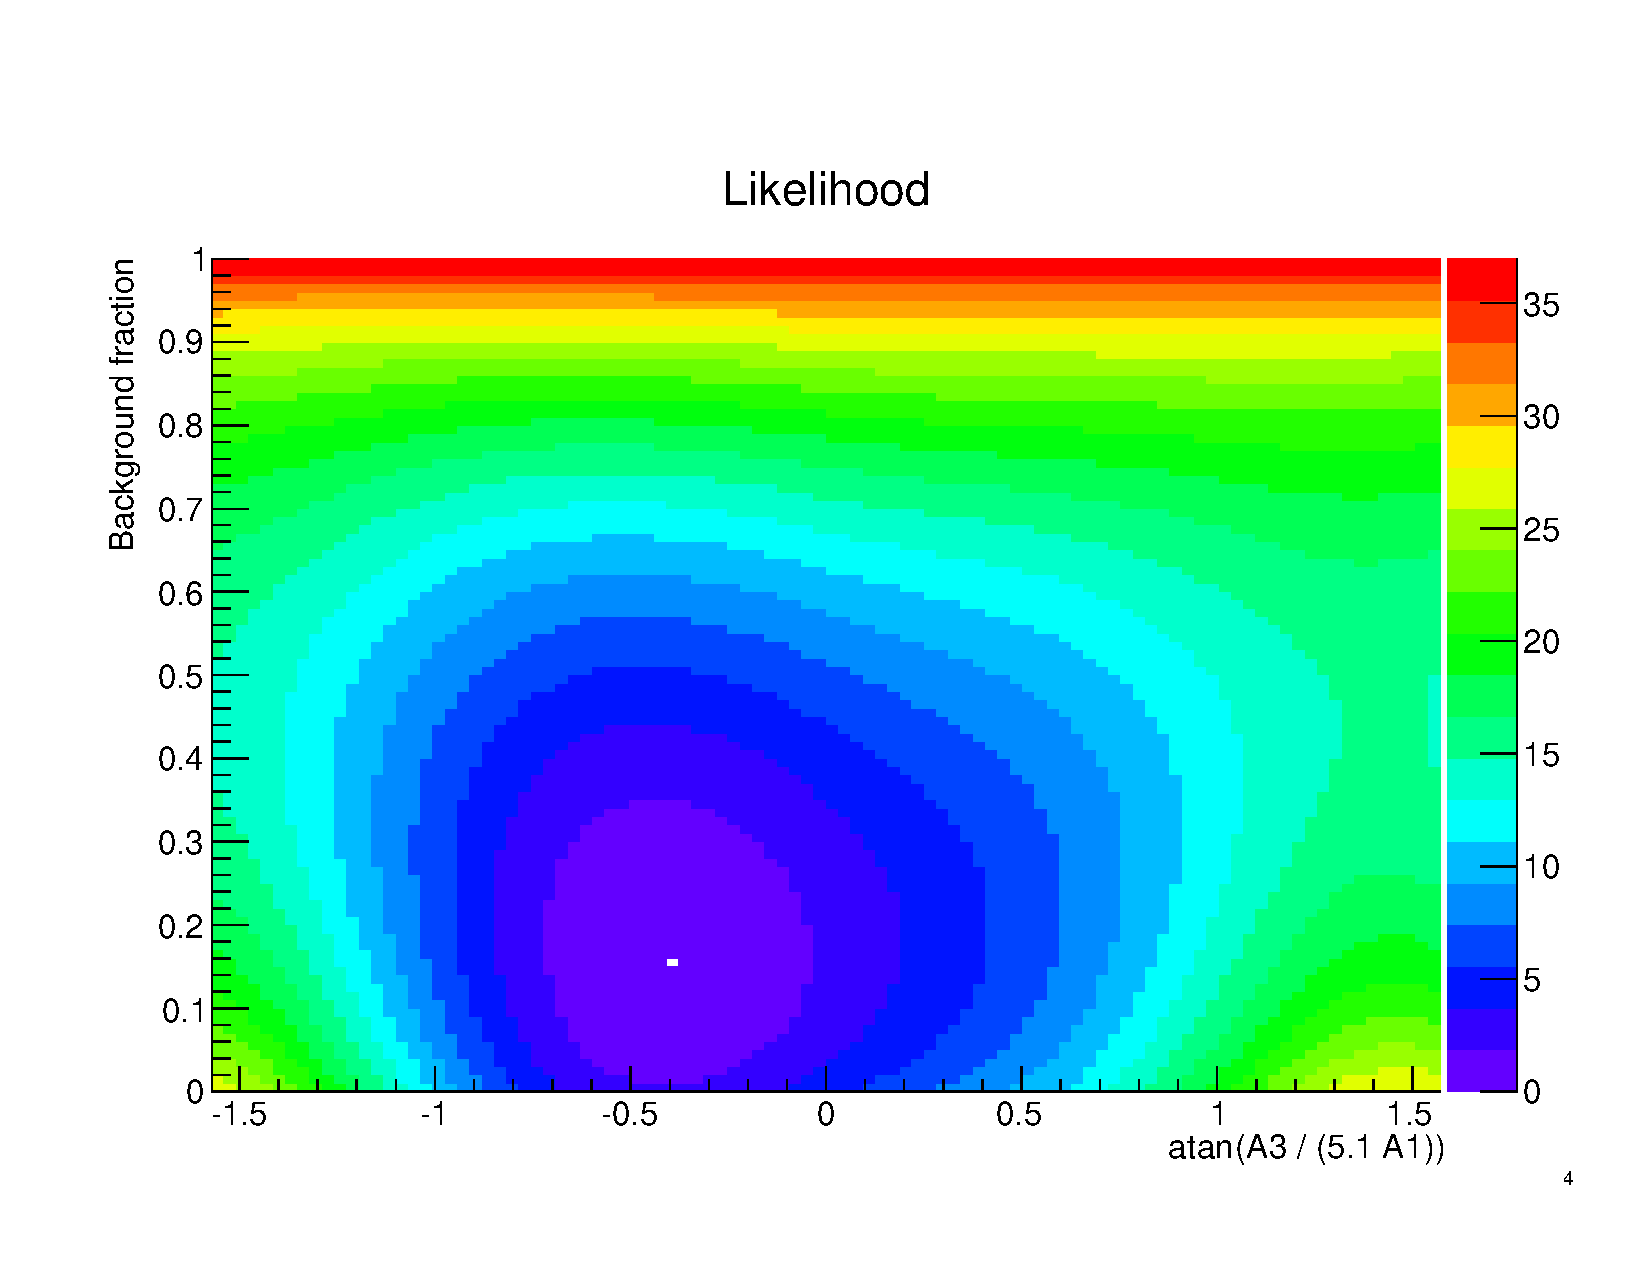
\includegraphics[width=0.48\textwidth]{figures/A1A3BNFit_LikelihoodExample.pdf}
    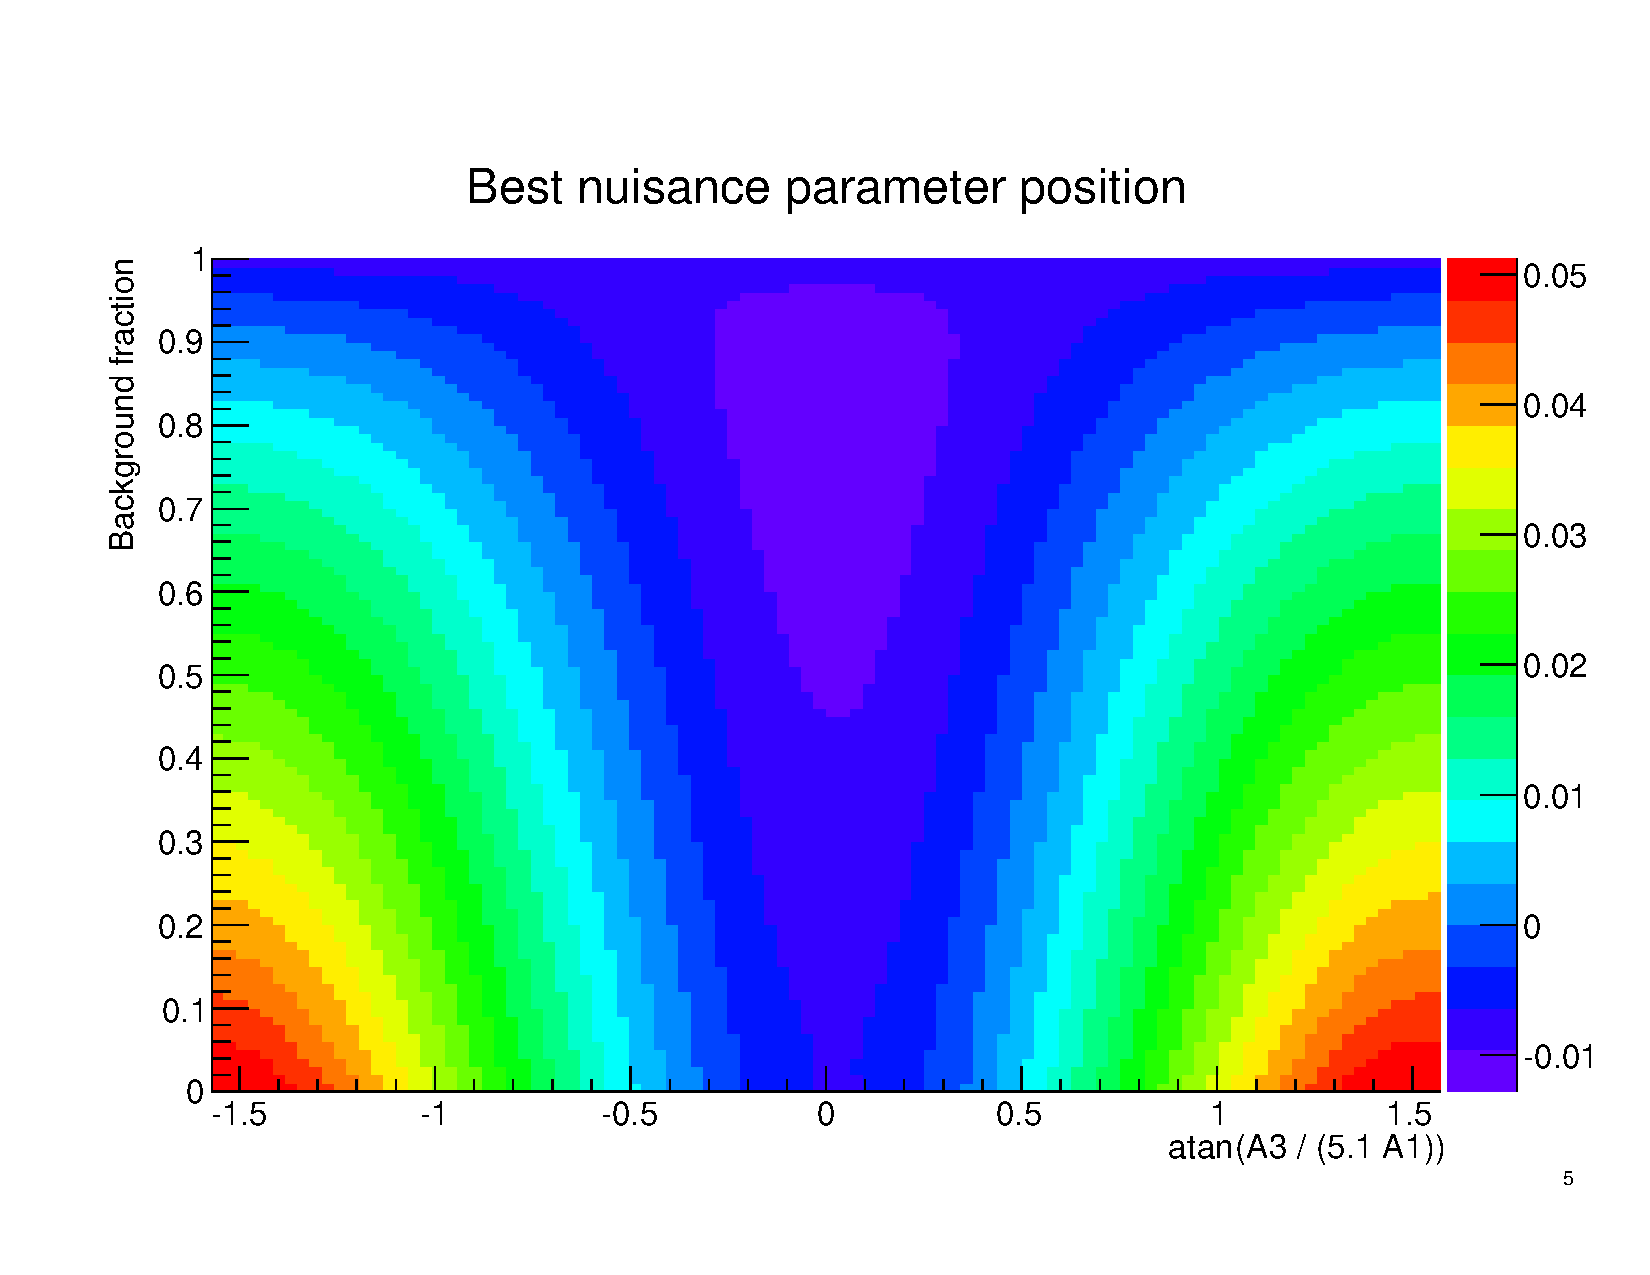
\includegraphics[width=0.48\textwidth]{figures/A1A3BNFit_NuisancePositionExample.pdf}
    \caption{Example likelihood scan for the signal (both $A_1^{ZZ}$ and $A_3^{ZZ}$) plus background fit
    with one nuisance parameter of a pseudo-dataset consists of 80 SM Higgs signal and 10 background events.
    On the right, best position for nuisance parameter is shown from the same fit, in units of sigmas}
    \label{fig:A1A3BNFitLikelihoodExample}
  \end{center}
\end{figure}


\section{Hybrid likelihood}

\subsection{General idea}

Since we do not need all the bins in the 8D space to do the fitting, we can do much better than the
brute-force way of filling all bins as described above.  In order to perform fitting, all we need
is a fast way to calculate the likelihood only for the events we want to fit.  This can be realized
by imaging that there is a tiny bin around each event in our interest, and spend time on calculating
the bin values for those bins only.  The integral of the whole ``invisible'' map is also needed,
but that can be pre-calculated on a grid once and for all.

With this being said, it's still a non-trivial task to calculate each single event in a reasonable
amount of time, and some simple approximations are needed.

\subsection{Integration in case of a flat ME}

The complication comes when we want to include lepton momentum resolution effects.  Let $m_{ij}$
denote the invariant mass between lepton $i$ and $j$, where leptons 1 and 2 make up the first Z
candidate, and 3 and 4 make up the second.  If each lepton $i$ is smeared by a smearing factor $c_i$,
in other word when we write in terms of the 4-momenta,

\begin{equation}
p'_i = c_i p_i,
\end{equation}

then the dilepton masses can be written (in the massless lepton limit) simply as

\begin{equation}
{m'}_{ij}^2 = (p'_i + p'_j)^2 = (c_i p_i + c_j p_j)^2 = c_i^2 p_i^2 + 2 c_i c_j p_i p_j + c_j^2 p_j^2
   = c_i c_j m_{ij}^2.
\end{equation}

As a consequence, when we are doing integral of the contribution from different masses to the target
dilepton mass, there is one integral per Z over $c_i$.  The integration to get ``bin'' value can be
written as

\begin{eqnarray}
V(\vec{X}) &=& \int\int F(m'_{12} \rightarrow m_{12} | \vec{X}) F(m'_{34} \rightarrow m_{34} | \vec{X}) d (m'_{12})^2 d (m'_{34})^2\\
F(m' \rightarrow m | \vec{X}) &=& \int f(c | \vec{X}) f\left(\left(\dfrac{m}{m'}\right)^2 \dfrac{1}{c}|\vec{X}\right) \epsilon\left(c, \left(\dfrac{m}{m'}\right)^2 \dfrac{1}{c} | \vec{X}\right) d c,
\end{eqnarray}

where $\epsilon(c_i, c_j | \vec{X})$ incorporates efficiency and acceptance effects from detector,
and $f(c | \vec{X})$ is the smearing function for lepton momenta.  Note that the $m_{4l}$ will also be
smeared, but it's ignored for now, and will be restored in the next section when we include ME back into the game.

A number of different approaches are probed to study the time vs. precision performance for the 4 nested integrals:
MC integration with uniform sampling, Gaussian sampling, uniform grid with Simpson's rule, uniform grid with
Boole's rule, adapted Simpson's rule and Boole's rule.  Their performance are summarized as follows:

\begin{enumerate}
\item The sampling integration ones are performing significantly worse than the quadrature counter-parts: ie.,
   we need a lot more time to reach similar precision.
\item Integration with Boole's rule with uniformly-spaced grid takes about 10 ms (without ME) to reach 1\% precision.
   With ME the time needed is estimated to be at least 250 times longer.
\item Adapted Simpson's rule has similar performance to adapted Boole's rule if we limit ourselves to 0.1\% precision.
   With fake ME evaluation in appropriate places, time spent is estimated to be 0.6 s per event for a 0.1\%
   top-level tolerance (inner integral have 1/10 tolerance than it's immediate parent integral, and initial
   division is 10).
\end{enumerate}

PS. I HAVE A LOT OF PLOTS FOR THESE ITEMS.  DO WE WANT TO CORE-DUMP EVERYTHING INTO THE NOTE?

Example of performace summary for adapted Simpson's is shown in figure \ref{fig:FlatMEAdaptedSimpsonsPrecisionVsTime}.

\begin{figure}[htb!]
  \begin{center}
    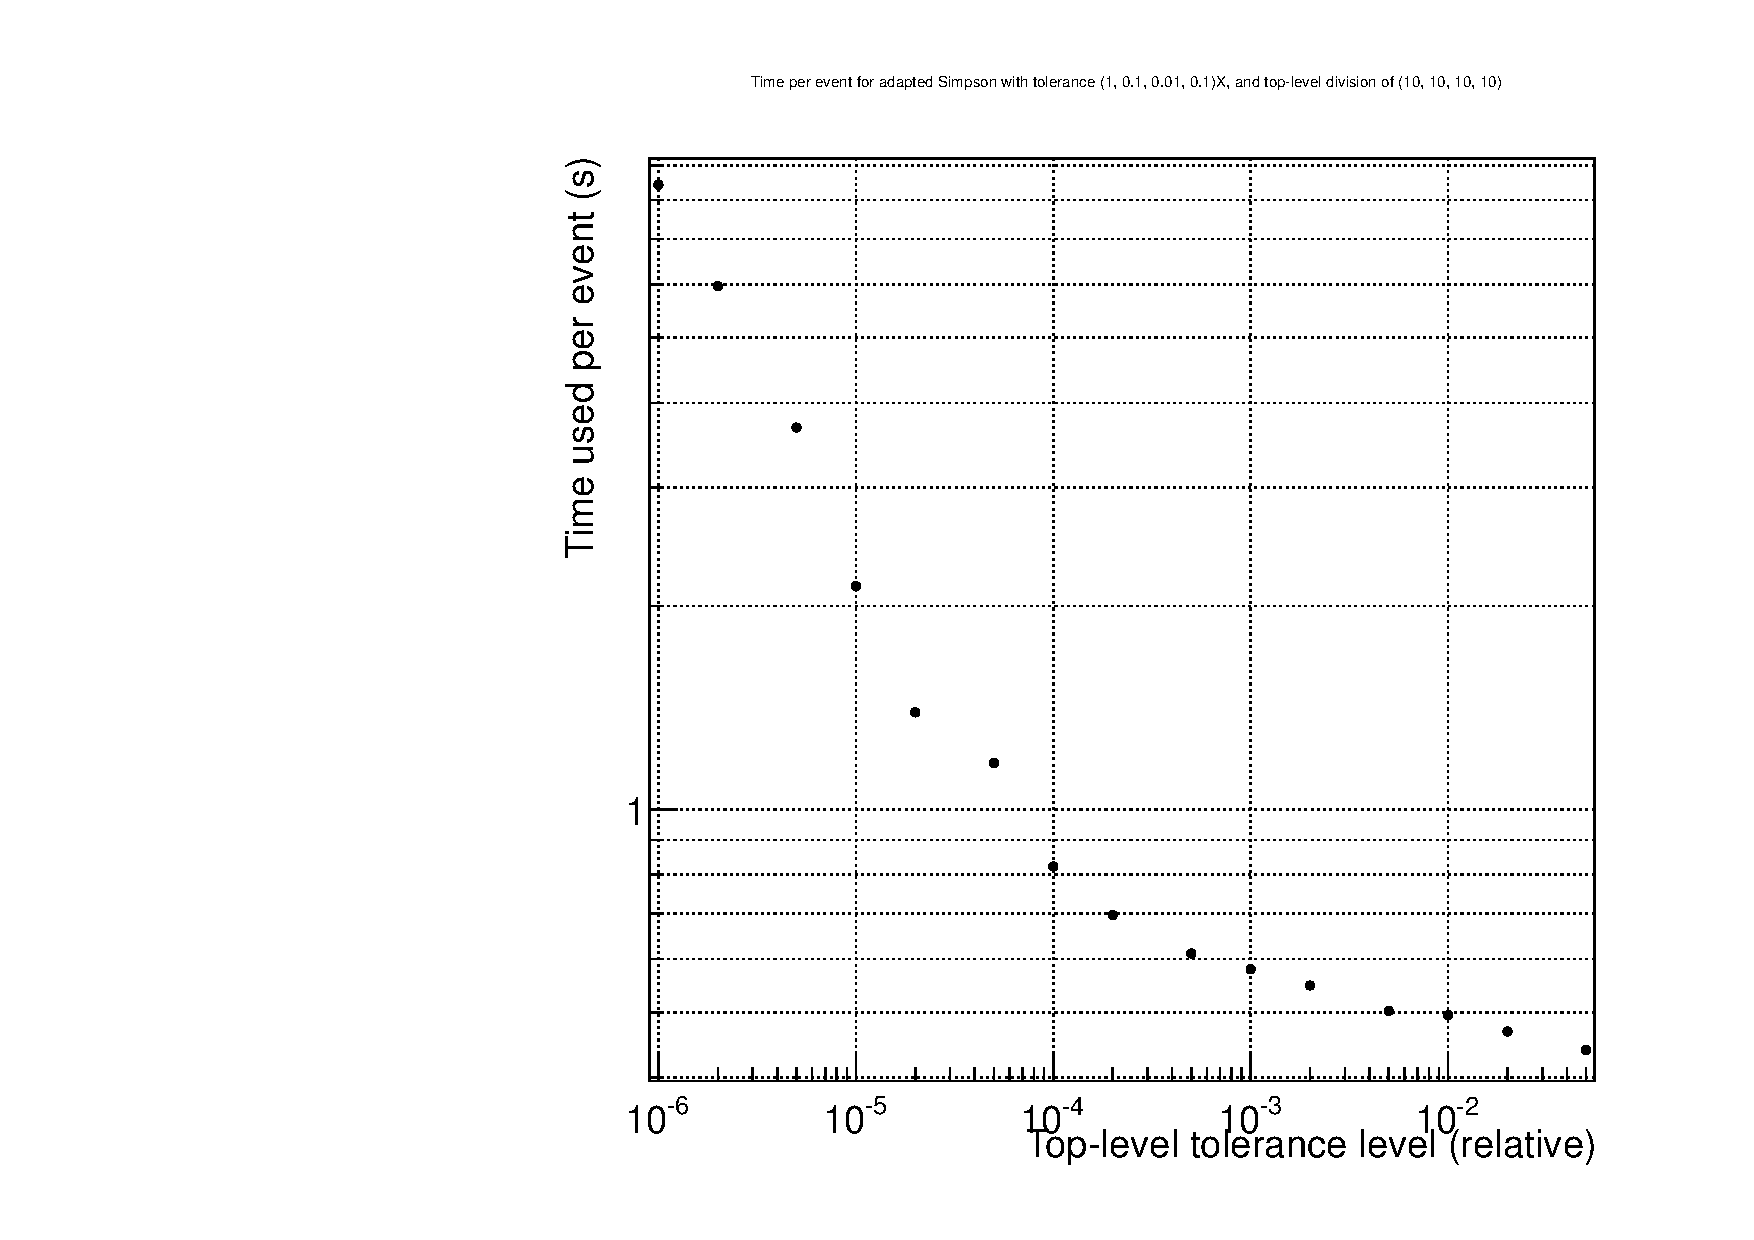
\includegraphics[width=0.48\textwidth]{figures/PrecisionVsTime_FlatME_AdaptedSimpsons.pdf}
    \caption{Time per event vs. precision for one example point in phase space using adapted Simpson's rule
    to perform numerical integration.  Tolerance level is relative to a quick-estimate of the integral, which
    is seen to be within O(20\%) to the final answer.}
    \label{fig:FlatMEAdaptedSimpsonsPrecisionVsTime}
  \end{center}
\end{figure}

\subsection{Including ME to leading order(s)}

If we were to blindly include ME into the game, the $F(...)$ integrals can no longer be integrated separately,
since the expression of ME depends on $m_1$, $m_2$ as well as $m_{4l}$, and $m_{4l}$ depends on the cross-talk
between all pairs of leptons.  If we define the deviations as follows,

\begin{eqnarray}
c_i &=& 1 + \delta_i\\
m'_{ij} &=& m_{ij} (1 - \delta_{ij}^m),
\end{eqnarray}

then it follows that

\begin{eqnarray}
\left(\dfrac{m_{ij}}{m'_{ij}}\right)\dfrac{1}{c_i} &\simeq& (1 + 2 \delta_{ij}^m) (1 - \delta_i)
   \simeq 1 + (2 \delta_{ij}^m - \delta_i)\\
{m_{4l}'}^2 &\simeq& m_{4l}^2 + \sum_{i>j} (\delta_i + \delta_j) m_{ij}^2\nonumber\\
   &\simeq& m_{4l}^2 + 2 \delta_{12}^m (m_{12}^2 + m_{23}^2 + m_{24}^2)
   + 2 \delta_{34}^m (m_{34}^2 + m_{14}^2 + m_{24}^2)\nonumber\\
   && + 2 \delta_1 (E_1 - E_2) m_{4l} + 2 \delta_3 (E_3 - E_4) m_{4l},
\end{eqnarray}

where $E_i$ is the energy of the lepton in the 4-lepton rest frame.  This is the first-order expression
assuming all the $\delta$'s are small (of order of few percent).  Given the resolution we have
on the leptons, this is not a bad assumption.  Eventually we need to evaluate the effect from this however.
The last equation gives us the dependence of $m_{4l}$ to small smearing of lepton momentum starting from
some small displaced di-lepton masses.  We have shown that the relative change on 4-lepton mass
due to smearing on leptons is smaller than $\delta_i$, and that expansion make sense when
$\delta_i$ is of order of few percents.  This also allows us to write the matrix element to first order as

\begin{equation}
ME(\delta_{12}^m, \delta_{34}^m, \delta_1, \delta_3, \vec{X}) =
ME(\delta_{12}^m, \delta_{34}^m, \delta_1 = 0, \delta_3 = 0, \vec{X})
+ B_1(\delta_{12}^m, \delta_{34}^m, \vec{X}) \delta_1 + B_3(\delta_{12}^m, \delta_{34}^m, \vec{X}) \delta_3.
\end{equation}

We can easily pre-calculate various components and store in an array before engaging in any integration,
and furthermore, if we define an augmented version of inner integral $F$ as

\begin{equation}
F^{(n)}(m' \rightarrow m) = \int f(c) f\left(\left(\dfrac{m}{m'}\right)^2\dfrac{1}{c}\right) (c-1)^n d c,
\end{equation}

the crazy integral can be simplified as follows:

\begin{eqnarray}
&& \int\int\int\int
f(c_1) f\left(\left(\dfrac{m_{12}}{m'_{12}}\right)^2\dfrac{1}{c_1}\right)
f(c_3) f\left(\left(\dfrac{m_{34}}{m'_{34}}\right)^2\dfrac{1}{c_3}\right)
ME(\delta_{12}^m, \delta_{34}^m, \delta_1, \delta_3, \vec{X}) d c_1 d c_3 d (m'_{12})^2 d (m_{34})^2\nonumber\\
&=& \int\int\int\int
f(c_1) f\left(\left(\dfrac{m_{12}}{m'_{12}}\right)^2\dfrac{1}{c_1}\right)
f(c_3) f\left(\left(\dfrac{m_{34}}{m'_{34}}\right)^2\dfrac{1}{c_3}\right)
\left[ME(...)|_{\delta_1 = 0, \delta_3 = 0} + B_1(...) \delta_1 + B_3(...) \delta_3\right] d c_1 d c_3 d {m'_{12}}^2 d {m'_{34}}^2\nonumber\\
&=& \int\int
F^{(0)}(m'_{12}\rightarrow m_{12}) F^{(0)}(m'_{34}\rightarrow m_{34}) ME(...)|_{\delta_1 = 0, \delta_3 = 0}\nonumber\\
&& + F^{(1)}(m'_{12}\rightarrow m_{12}) F^{(0)}(m'_{34}\rightarrow m_{34}) B_1(...)
 + F^{(0)}(m'_{12}\rightarrow m_{12}) F^{(1)}(m'_{34}\rightarrow m_{34}) B_3(...) d {m'_{12}}^2 d {m'_{34}}^2.
\end{eqnarray}

For each event that we want to calculate likelihood for, $F^{(n)} (m' \rightarrow m)$ can also be pre-calculated.
In this fashion the integral become feasible again.  There are a couple remarks on this function $F^{(n)}$.
First, even though I didn't write out the dependence on the angles to save space, $F^{(n)}$'s are different
from event to event, and we need to recalculate those for each event.  Another point is that with this
final form, it is pretty easy to generalize into higher orders: there will be terms like $F^{(0)}F^{(2)}$,
$F^{(1)}F^{(1)}$, and so on.  Examples of the $F^{(n)}$ functions for an example point is shown in figure
\ref{fig:ExampleFFunctions}.

\begin{figure}[htb!]
  \begin{center}
    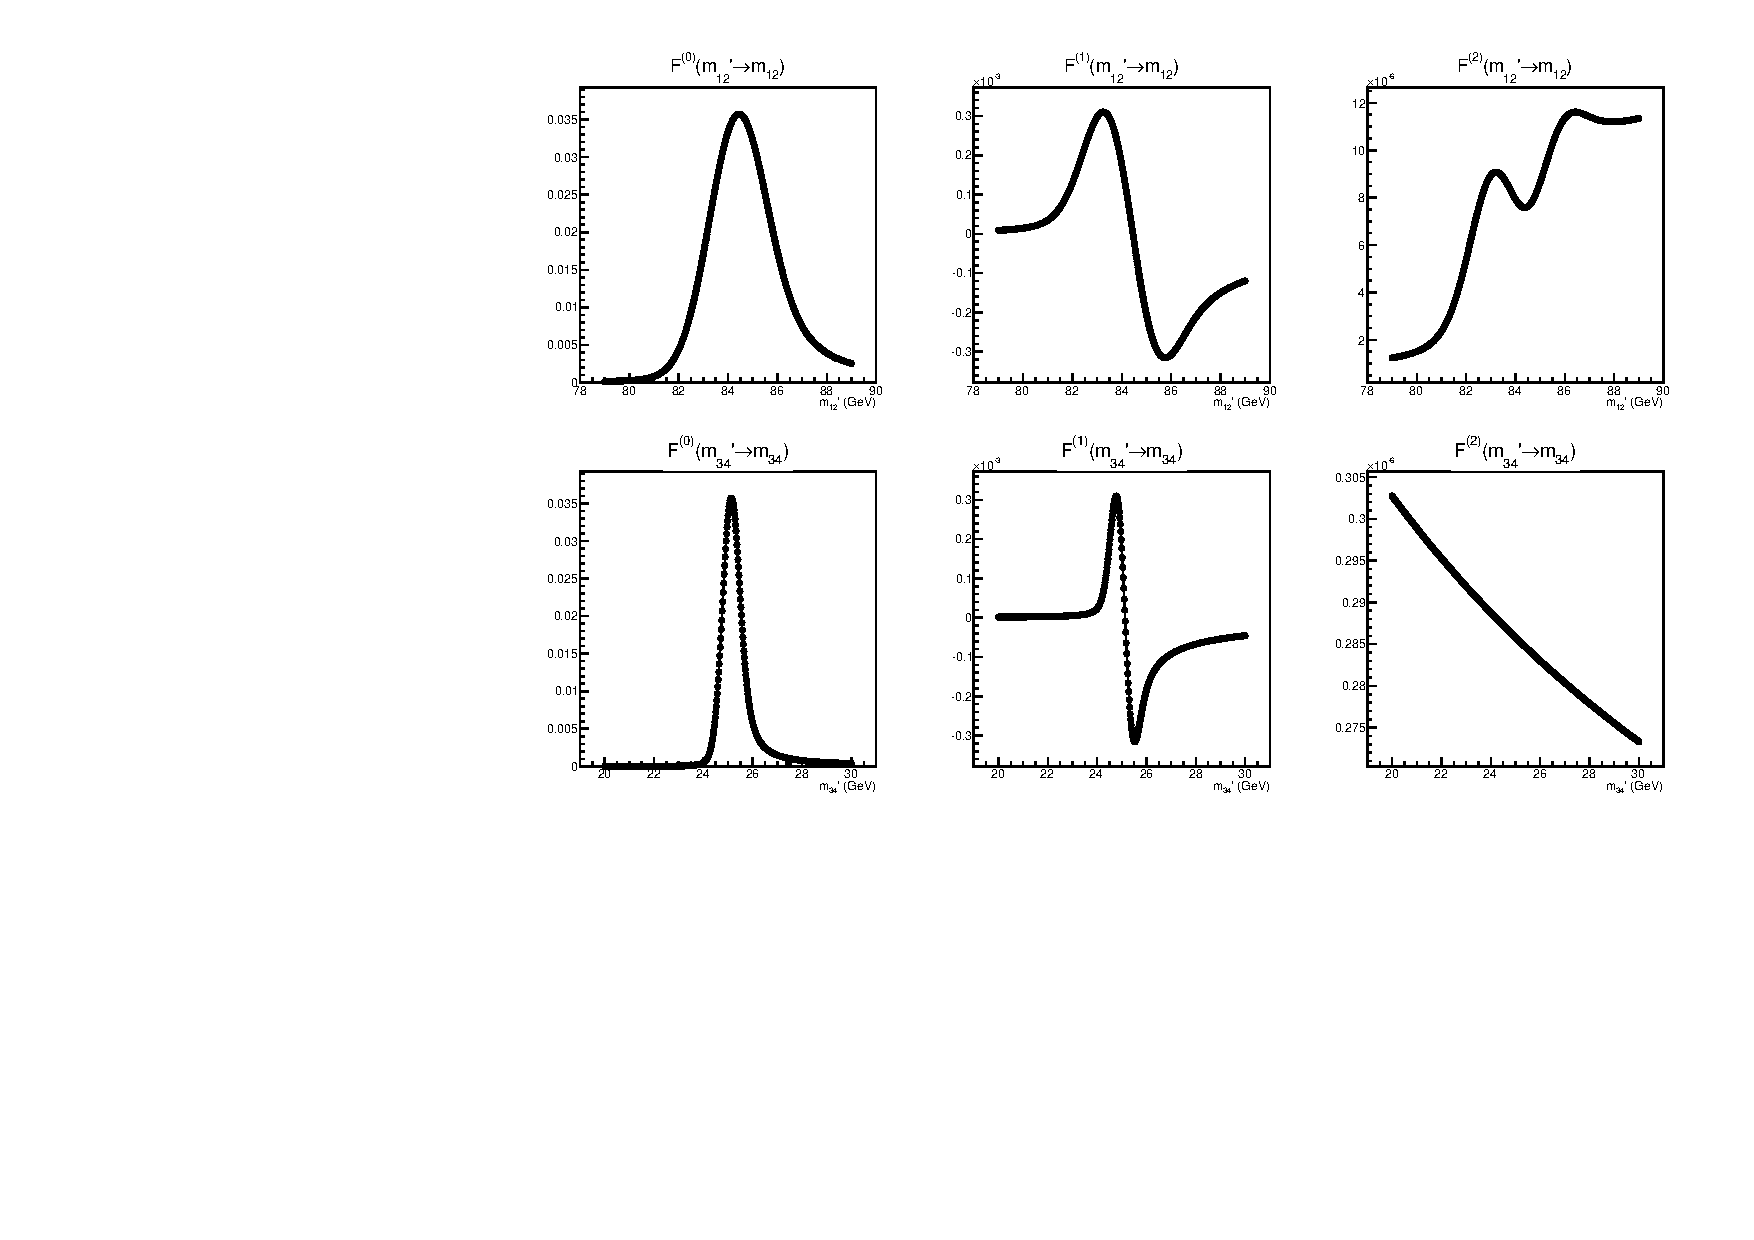
\includegraphics[width=0.85\textwidth]{figures/ExampleFFunction.pdf}
    \caption{Example $F^{(n)}$ functions for one point in phase space ($m_{4l} = 125$, $m_{12} = 84$, $m_{34} = 25$,
    $\Phi = 2.1$, $\cos(\Theta) = 0.92$, $\phi = 2.03$, $\cos(\theta_1) = 0.02$, $\cos(\theta_2) = -0.02$,
    with example smearing of lepton 1 ($\mu = 1$, $\sigma = 0.02$, $\alpha_L = 1.7$, $\alpha_R = 2.5$,
    $n_L = 1.49$, $n_R = 2.06$) and lepton 2 ($\mu = 0.99$, $\sigma = 0.02$, $\alpha_L = 1.7$, $\alpha_R = 2.5$,
    $n_L = 1.49$, $n_R = 2.06$)).  Tolerance in this plot are down to $10^{-5}$, $10^{-9}$ and $10^{-14}$ for different
    values of $n$ respectively.  Note the small-ness of the higher-order functions compared to $F^{(0)}$.}
    \label{fig:ExampleFFunctions}
  \end{center}
\end{figure}





\section{Systematics}

\section{Conclusion}

Conclusion


%===================================================================================================
\clearpage

\vspace*{-0.2cm}
\thebibliography{12}

\bibitem{ZeeTagAndProbeEGamma}
 CMS AN-2012/116, ``Tag and probe methodology for analyses using electrons and photons'',
CMS Egamma ID Group.

\bibitem{ZeeTagAndProbe2010}
 CMS AN-2010/464, ``Electron and muon efficiency measurements in 2010 proton-proton dataset'',
G. Bauer \textit{et al.}.

\bibitem{ZeeTagAndProbeTool}
 CMS AN-2009/111, ``Generic Tag and Probe Tool for Measuring Efficiency at CMS with Early Data'',
N. Adam \textit{et al.}.

\bibitem{VGammaPaper}
S. Chatrchyan \textit{et al.}, ``Measurement of W$\gamma$ and Z$\gamma$ production in pp collisions at $\sqrt{s}$ = 7 TeV'', Physiscs Letters B, vol. 701 pp535-555, 2011.

\bibitem{VGammaCMSNote}
CMS AN-2011/251, ``Study of Wgamma and Zgamma production at CMS with sqrt(s) = 7 TeV'', 
A. Askew \textit{et al.}.
%===================================================================================================

\appendix
\appendixpage

\section{Electron Response Functions}
\label{sec:ElectronResponseFunctions}


\begin{figure}[htb!]
  \begin{center}
    \subfigure[$|\eta| < 0.2$]{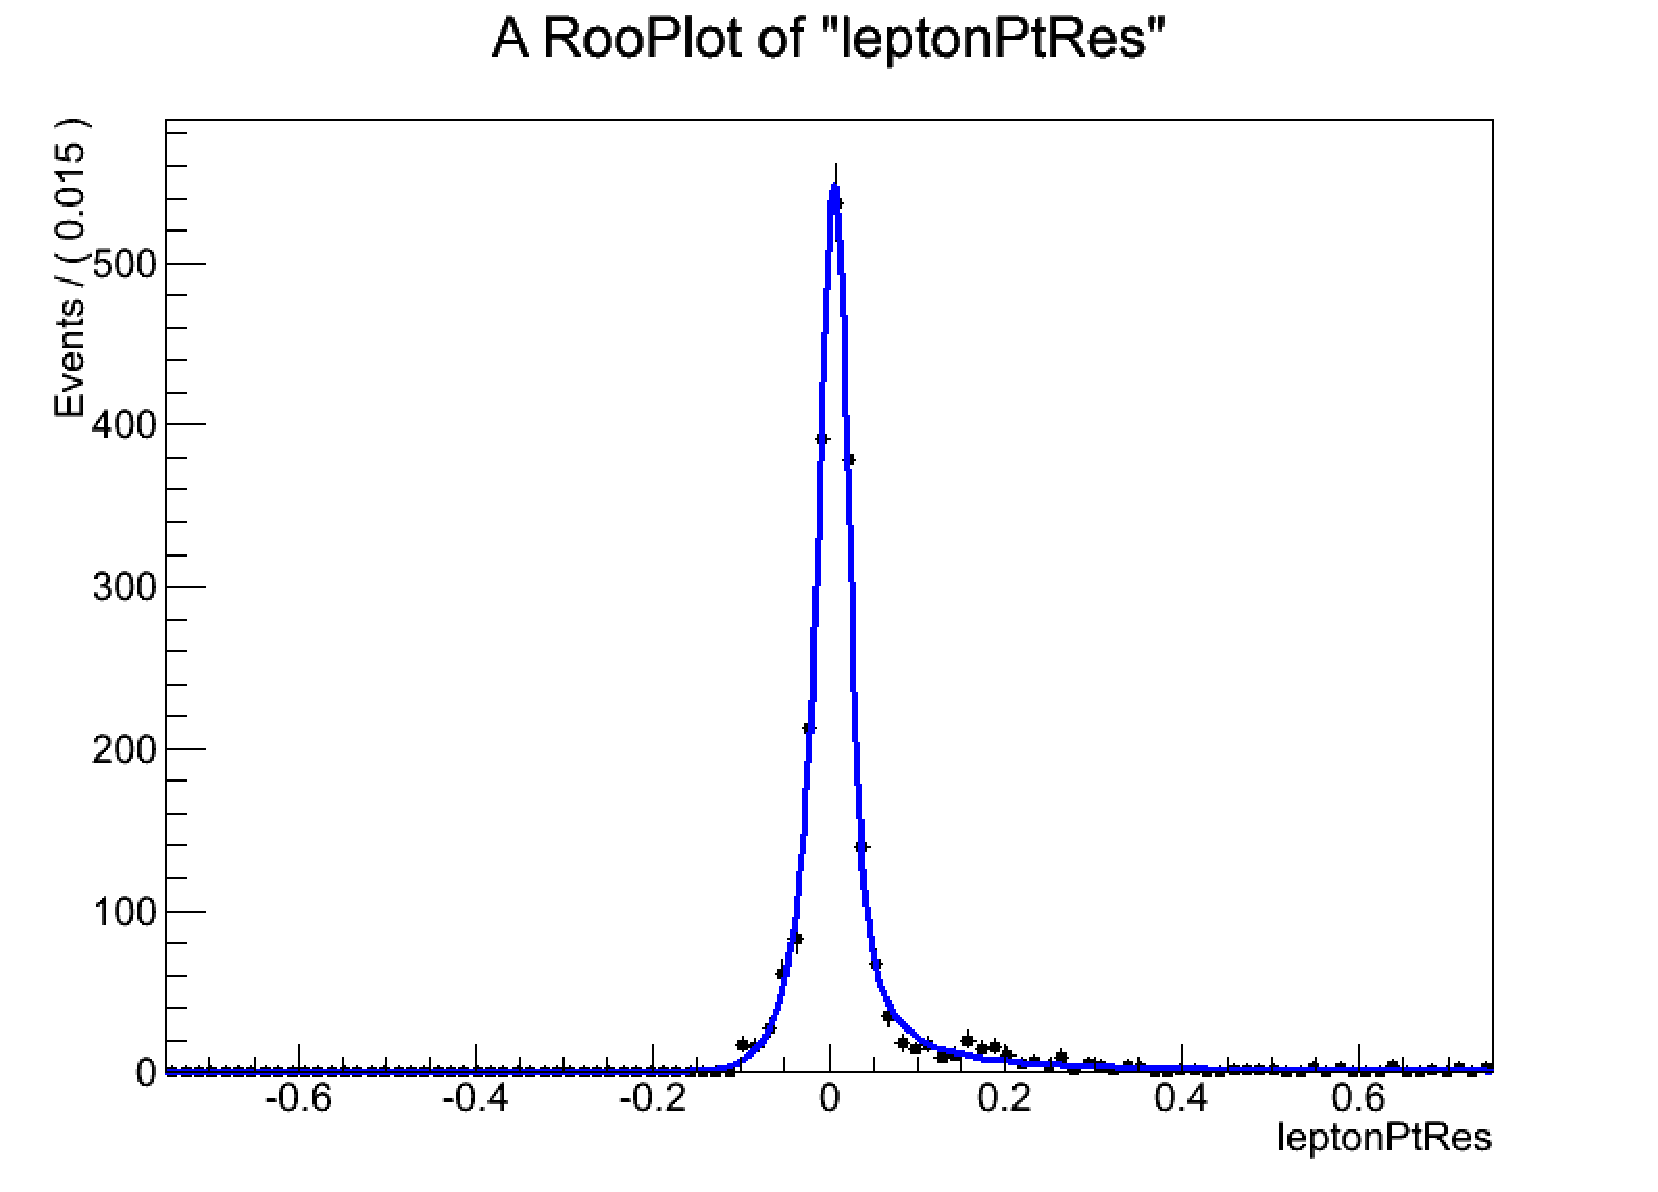
\includegraphics[width=0.245\textwidth]{figures/LeptonPtResolution_Electrons_PtBin2_EtaBin1.pdf}}
    \subfigure[$0.2 \le |\eta| < 0.4$]{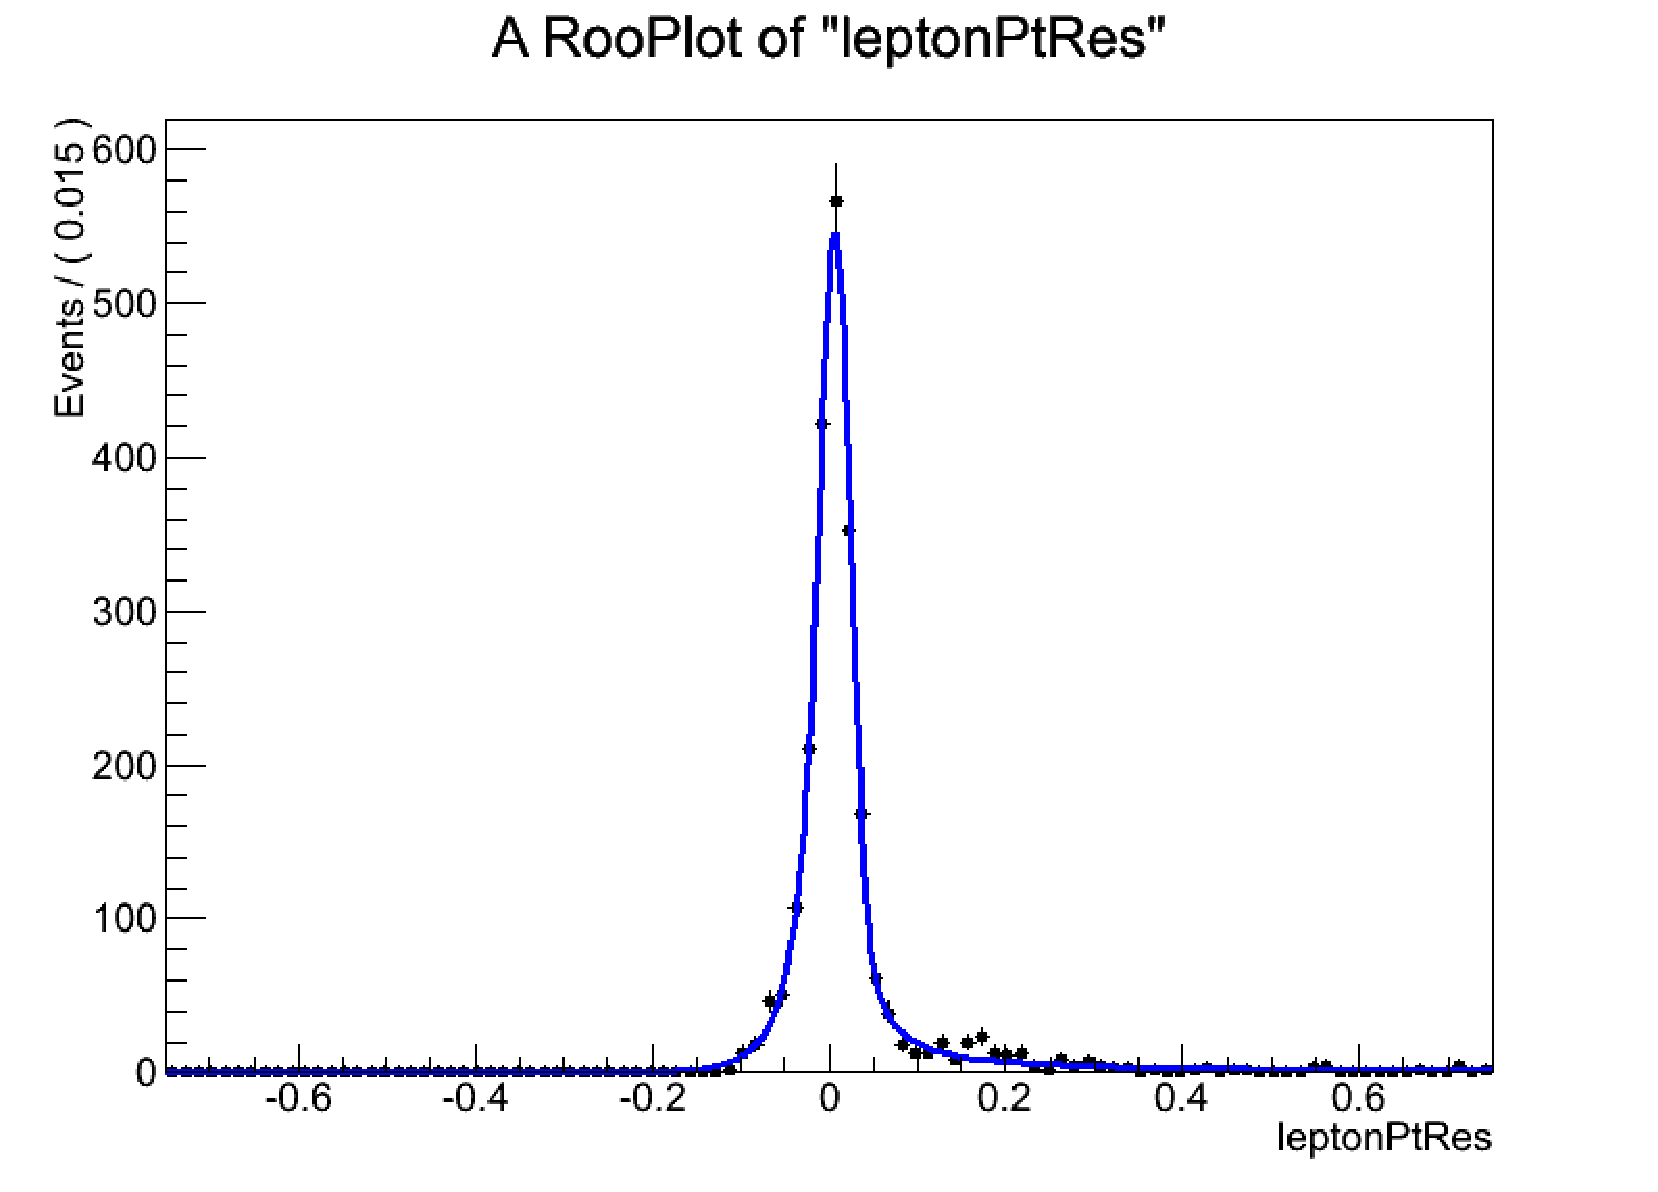
\includegraphics[width=0.245\textwidth]{figures/LeptonPtResolution_Electrons_PtBin2_EtaBin2.pdf}}
    \subfigure[$0.4 \le |\eta| < 0.6$]{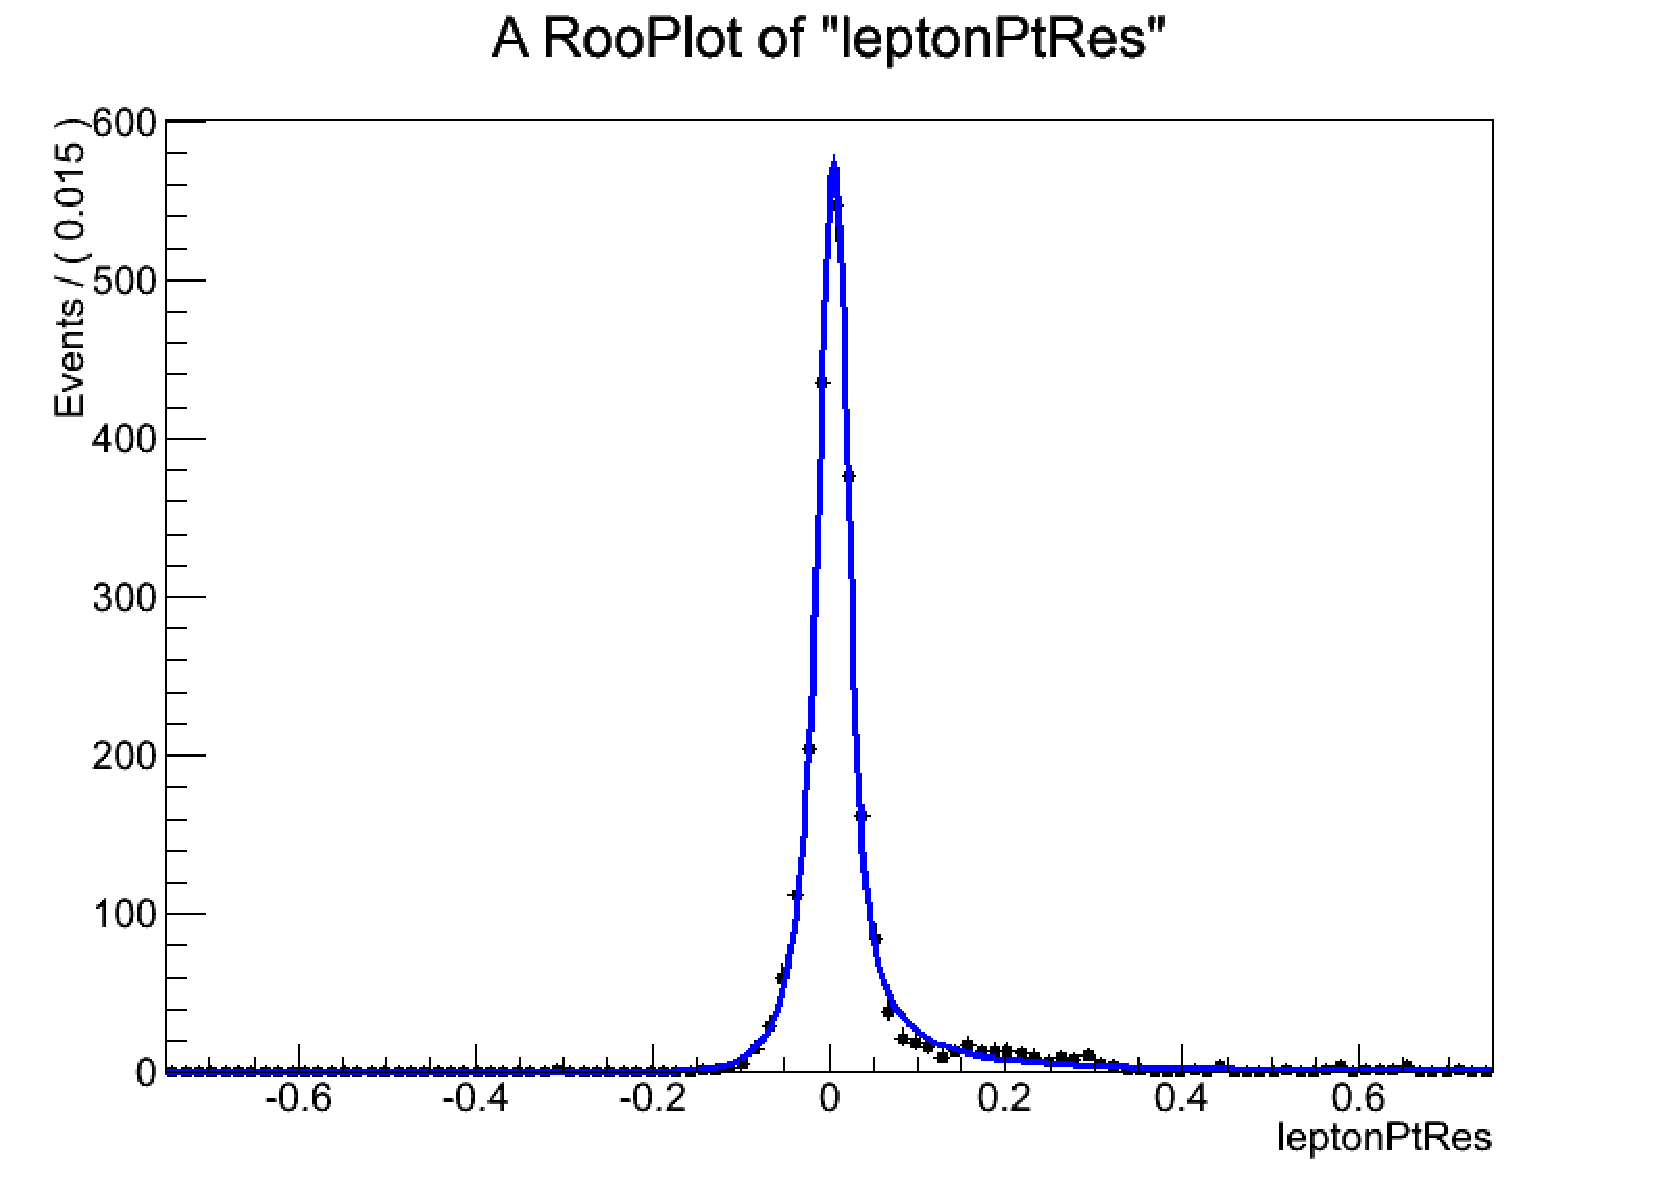
\includegraphics[width=0.245\textwidth]{figures/LeptonPtResolution_Electrons_PtBin2_EtaBin3.pdf}}
    \subfigure[$0.6 \le |\eta| < 0.8$]{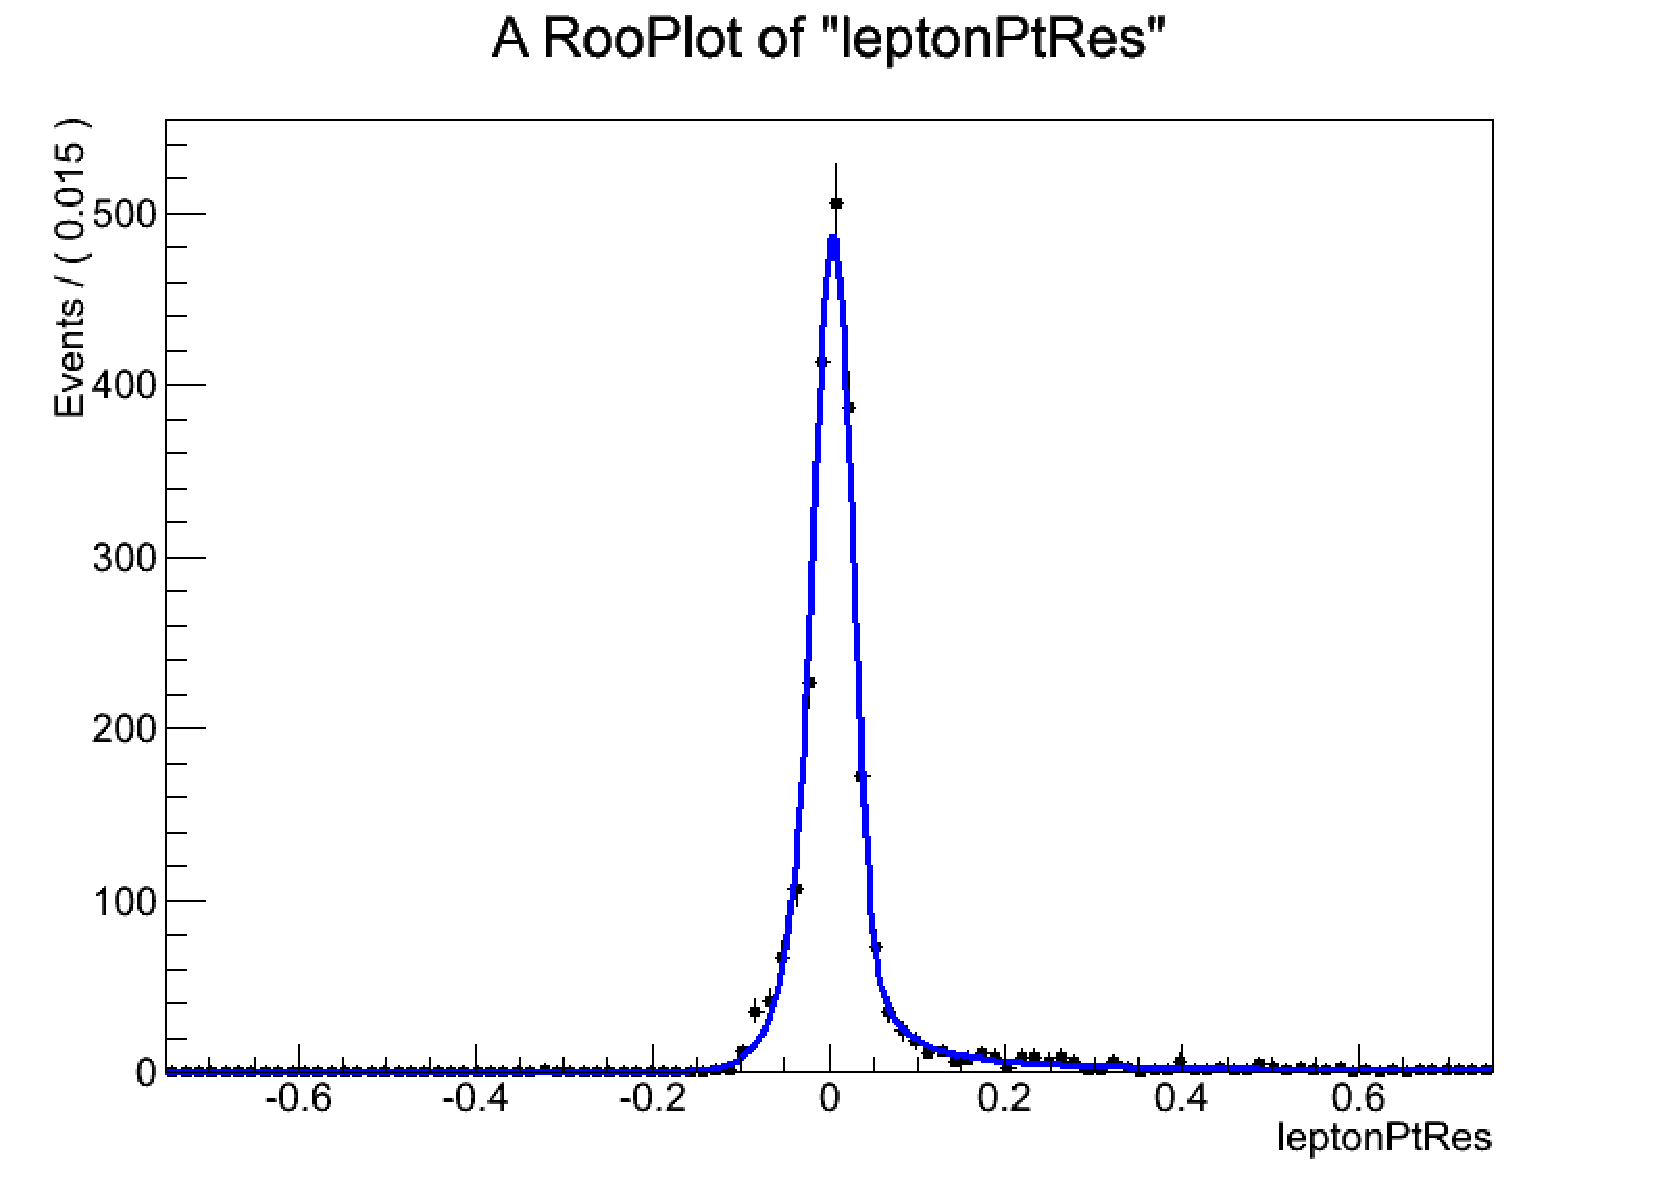
\includegraphics[width=0.245\textwidth]{figures/LeptonPtResolution_Electrons_PtBin2_EtaBin4.pdf}}
    \subfigure[$0.8 \le |\eta| < 1.0$]{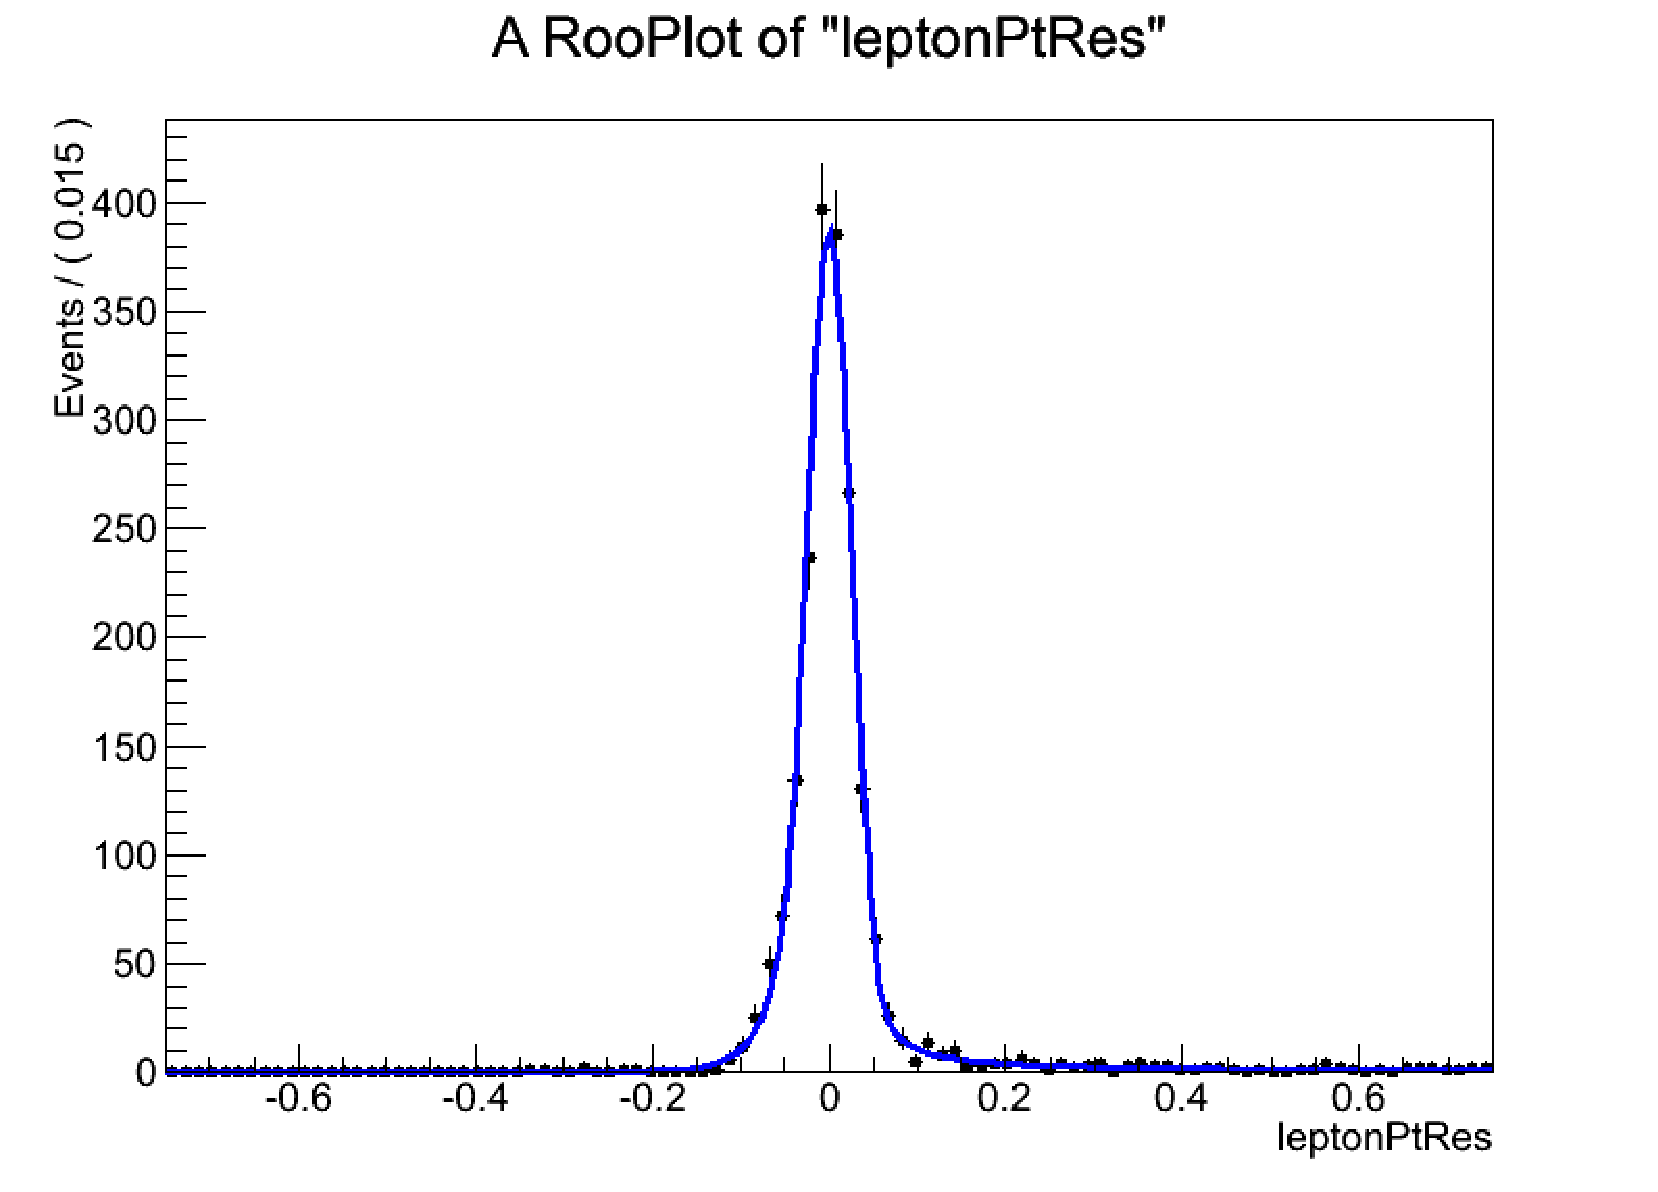
\includegraphics[width=0.245\textwidth]{figures/LeptonPtResolution_Electrons_PtBin2_EtaBin5.pdf}}
    \subfigure[$1.0 \le |\eta| < 1.2$]{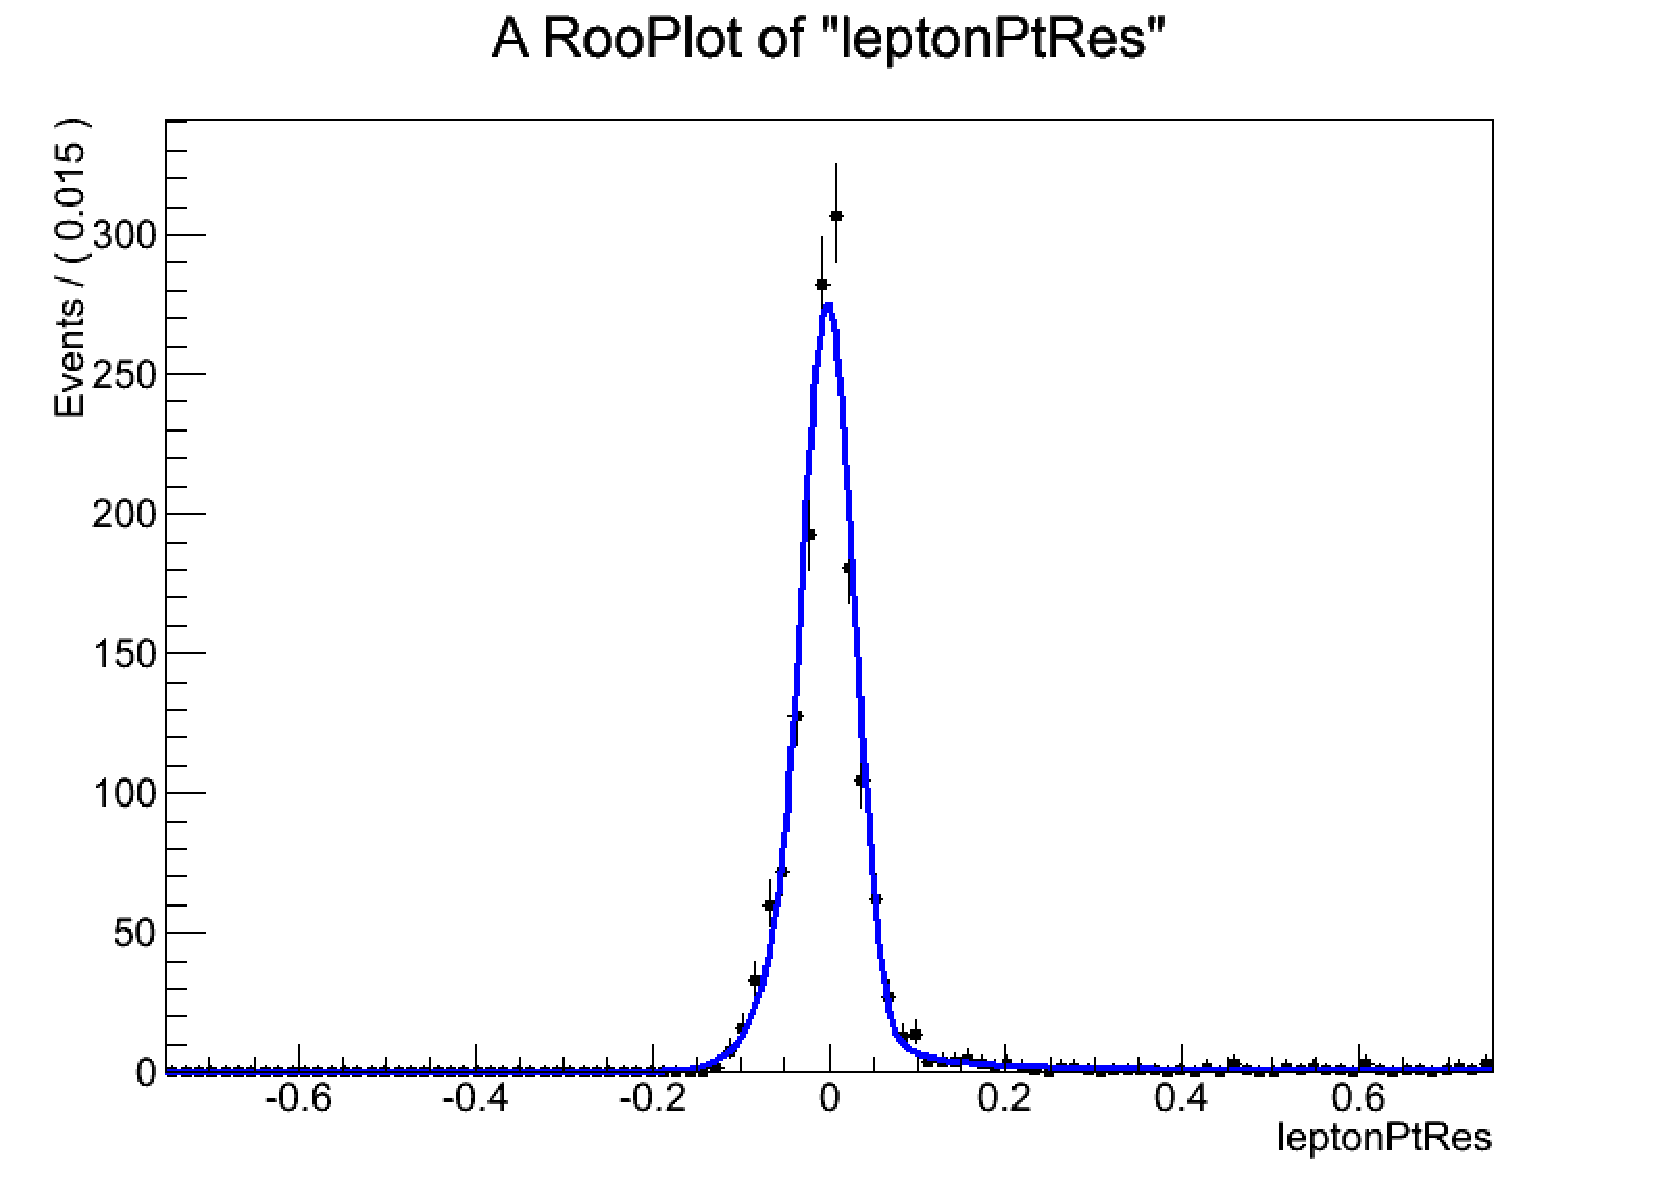
\includegraphics[width=0.245\textwidth]{figures/LeptonPtResolution_Electrons_PtBin2_EtaBin6.pdf}}
    \subfigure[$1.2 \le |\eta| < 1.4442$]{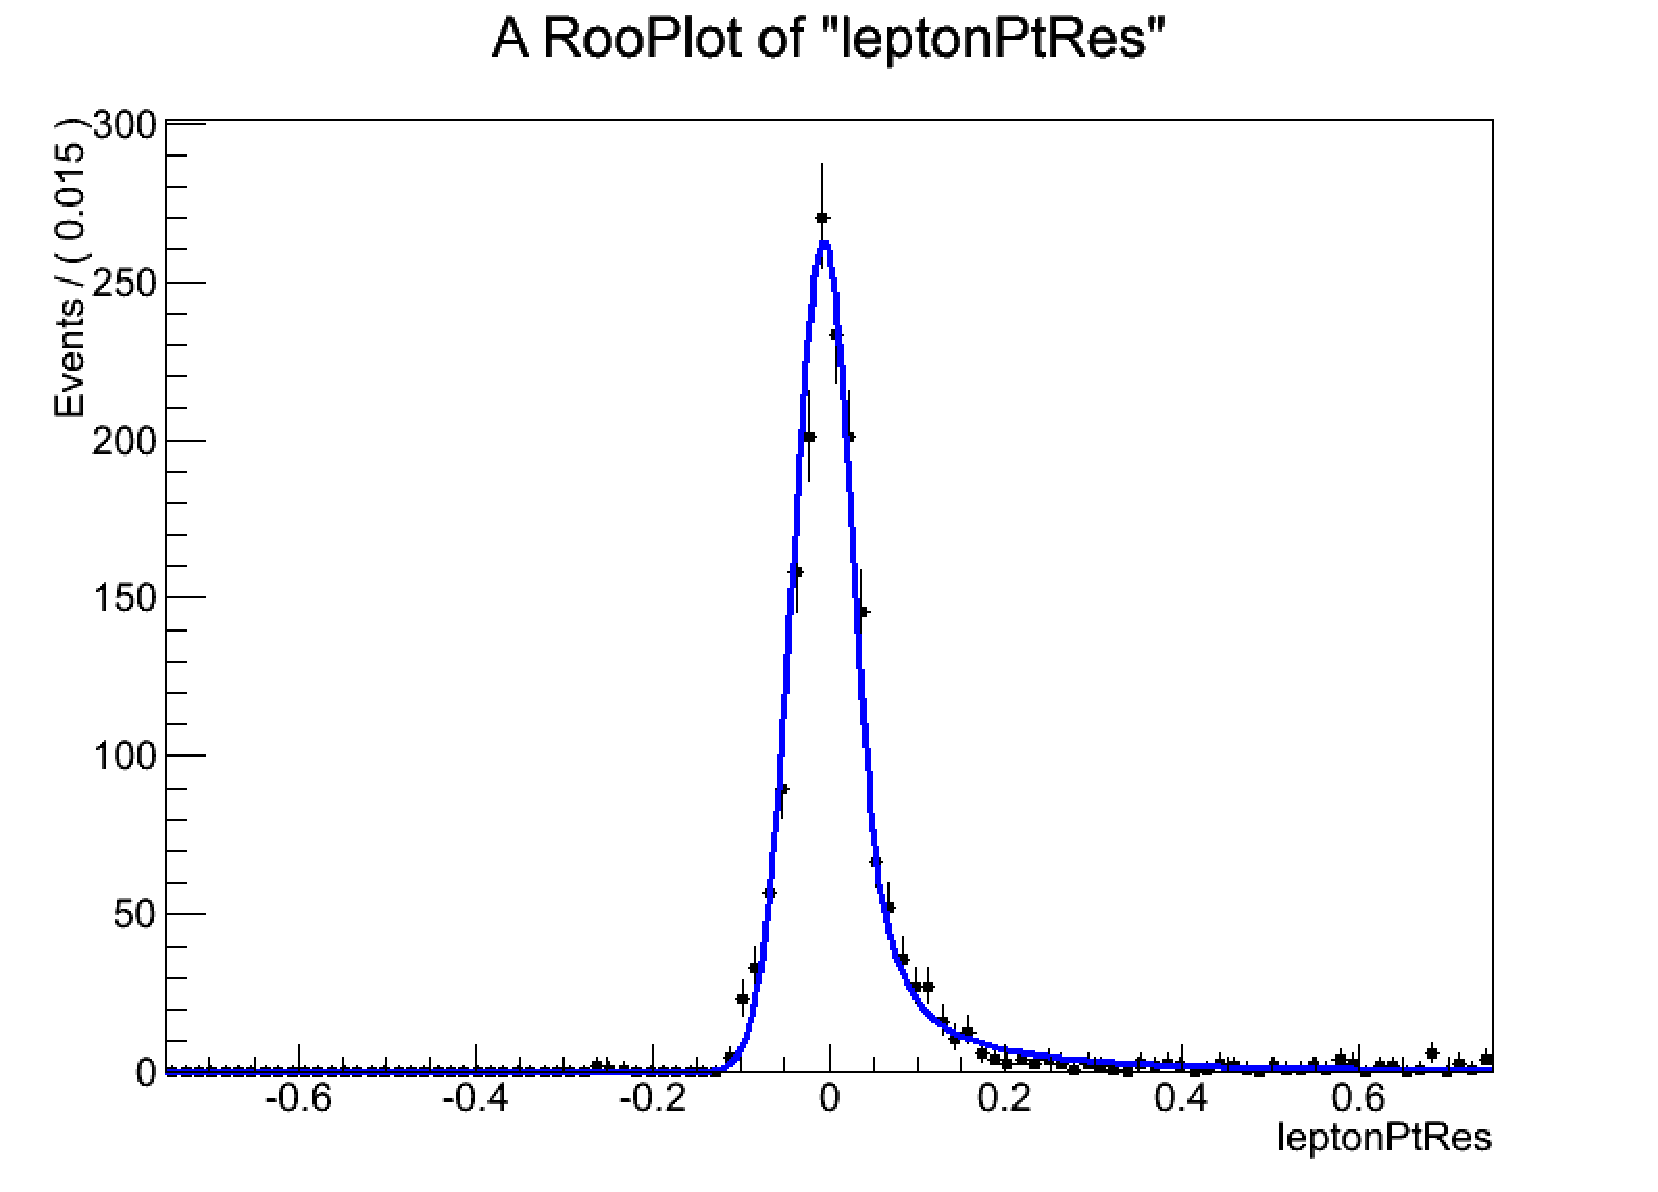
\includegraphics[width=0.245\textwidth]{figures/LeptonPtResolution_Electrons_PtBin2_EtaBin7.pdf}}
    \subfigure[$1.4 \le |\eta| < 1.566$]{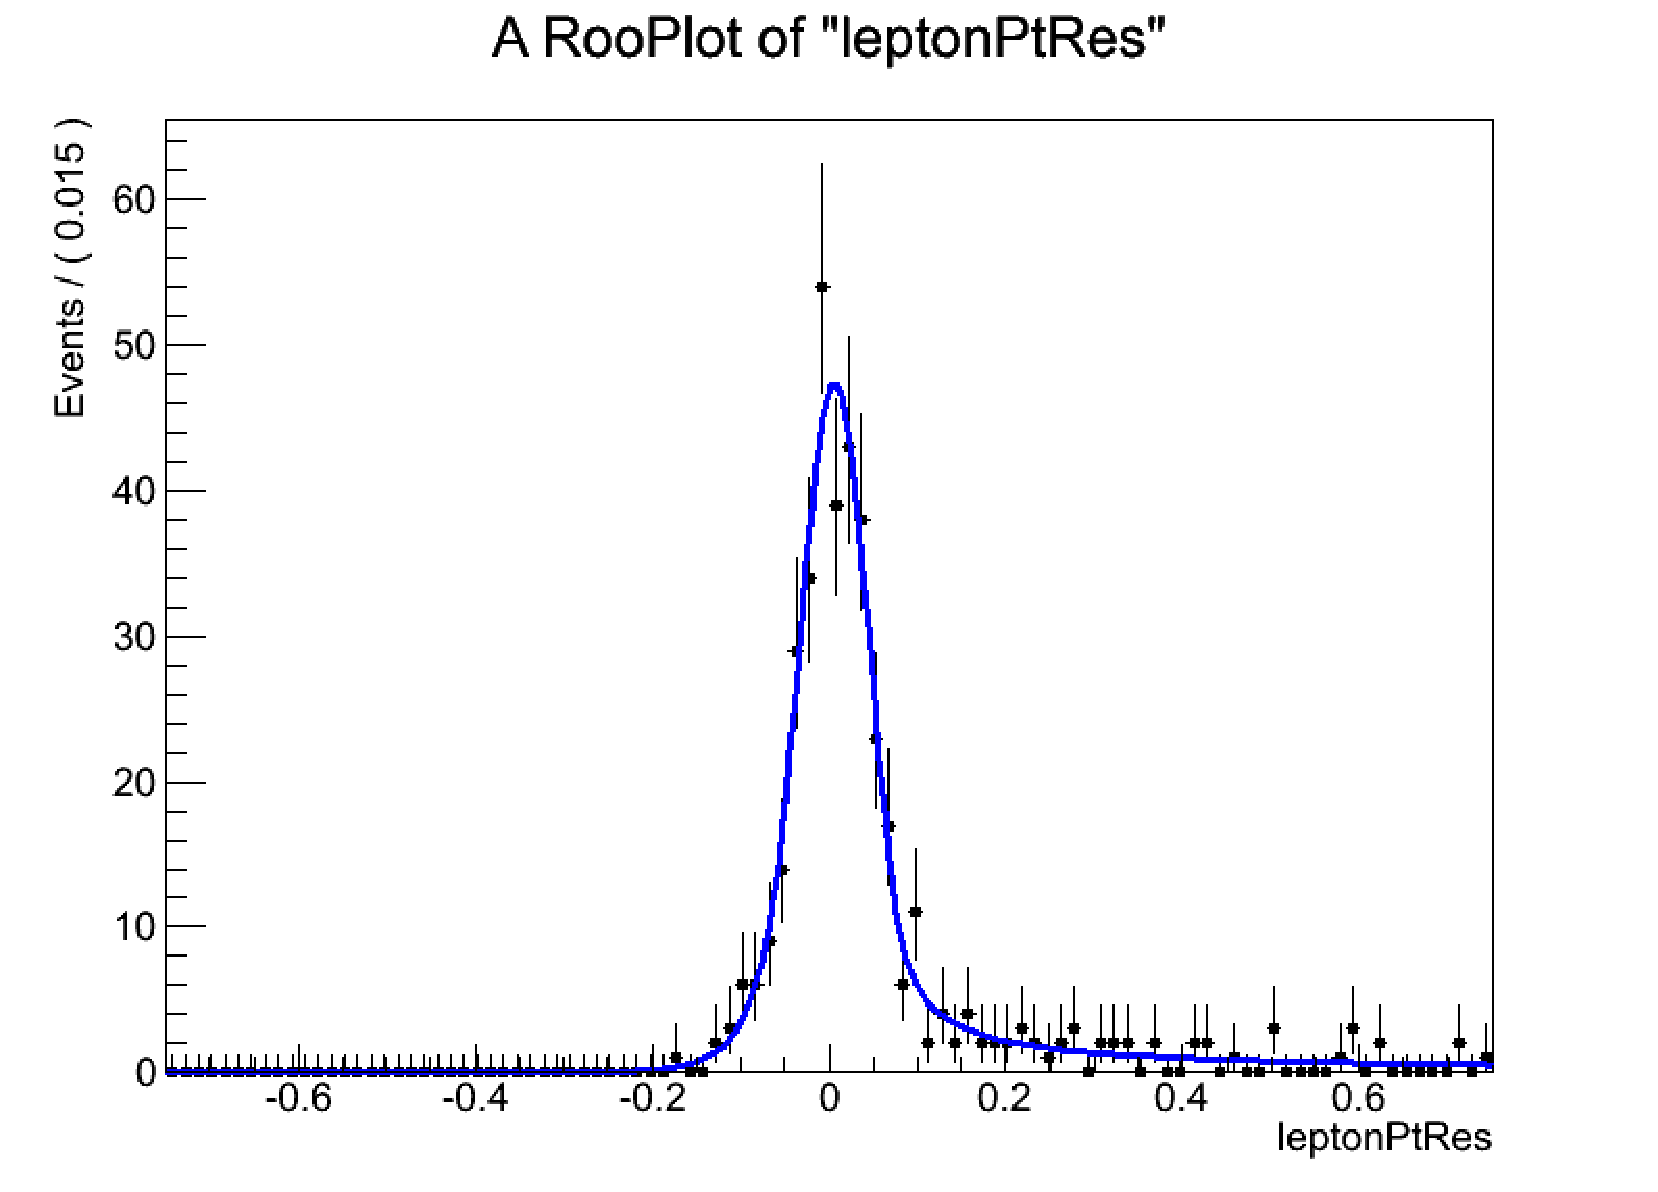
\includegraphics[width=0.245\textwidth]{figures/LeptonPtResolution_Electrons_PtBin2_EtaBin8.pdf}}
    \caption{ Energy response histogram and fitted response function for barrel electrons with $p_{T}$ between 
      $7$~\GeV and $8$~\GeV 
    }
    \label{fig:ElectronResponse_PtBin2_Barrel}
  \end{center}
\end{figure}

\begin{figure}[htb!]
  \begin{center}
    \subfigure[$1.566 \le |\eta| < 1.8$]{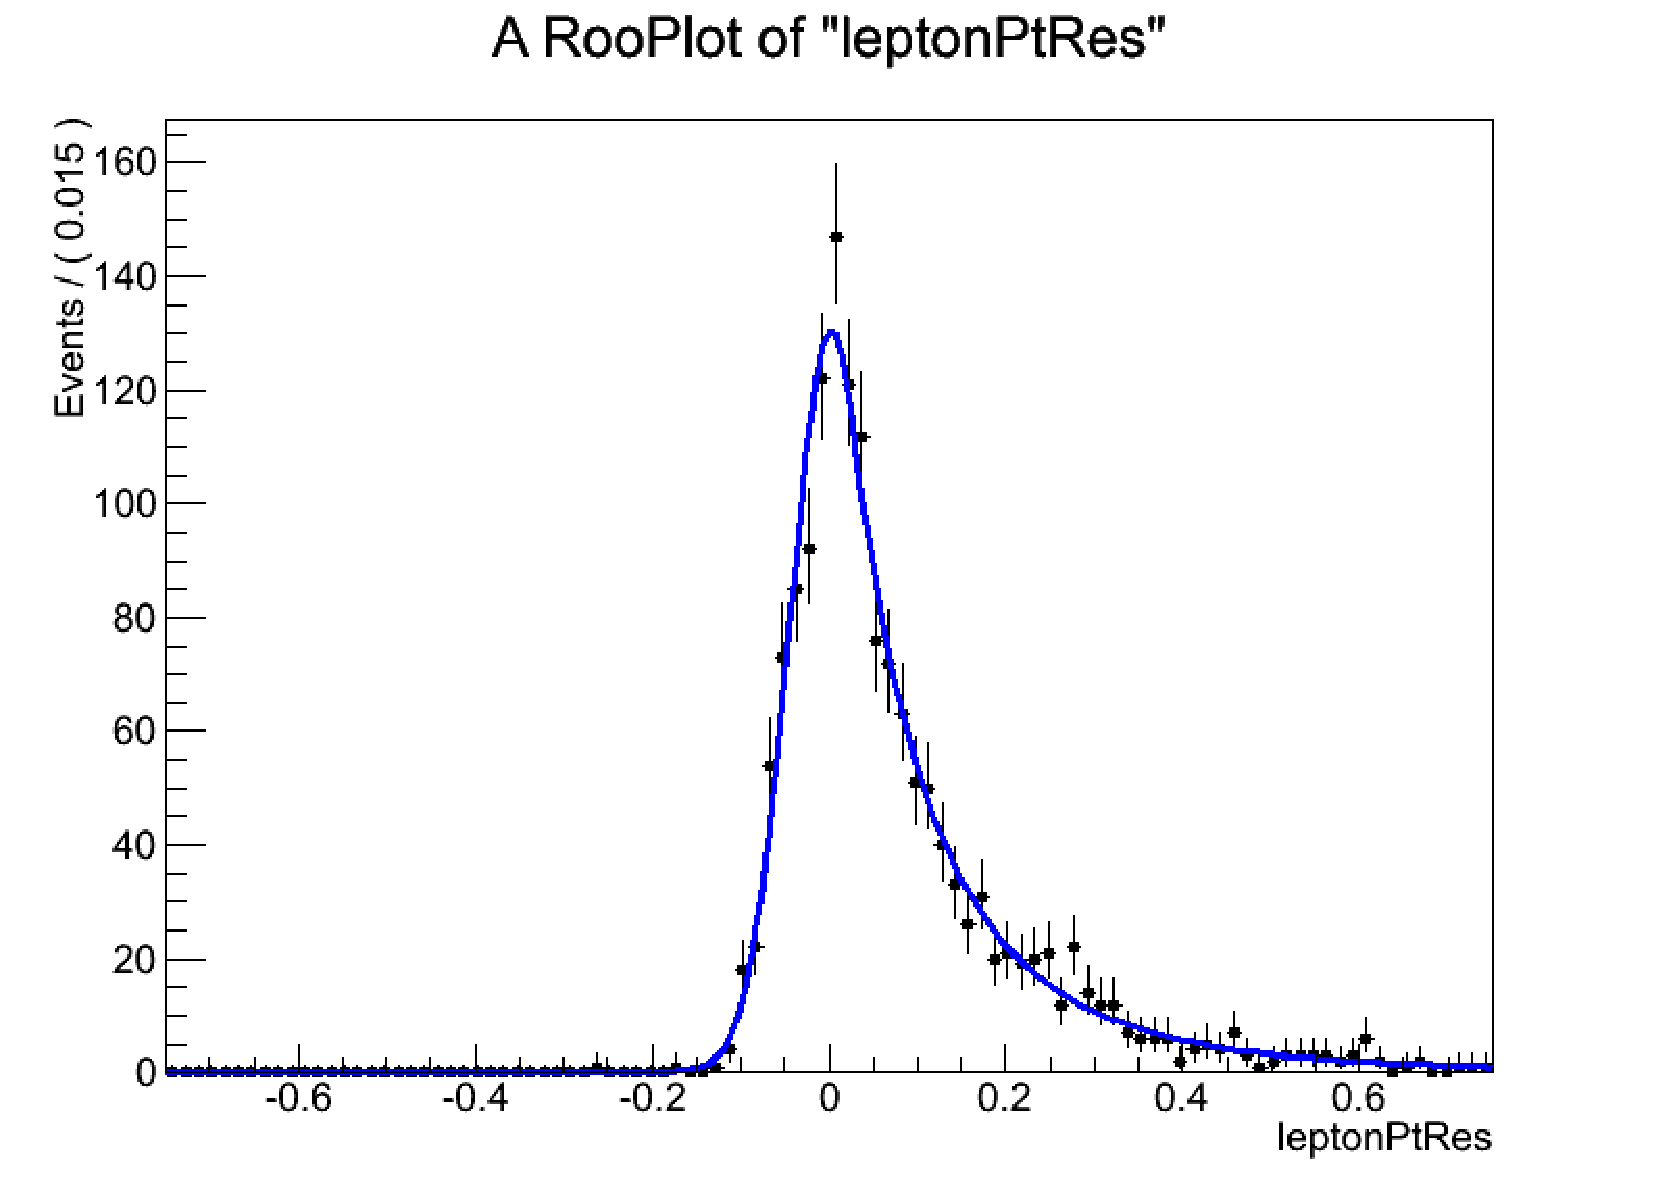
\includegraphics[width=0.245\textwidth]{figures/LeptonPtResolution_Electrons_PtBin2_EtaBin9.pdf}}
    \subfigure[$1.8 \le |\eta| < 2.0$]{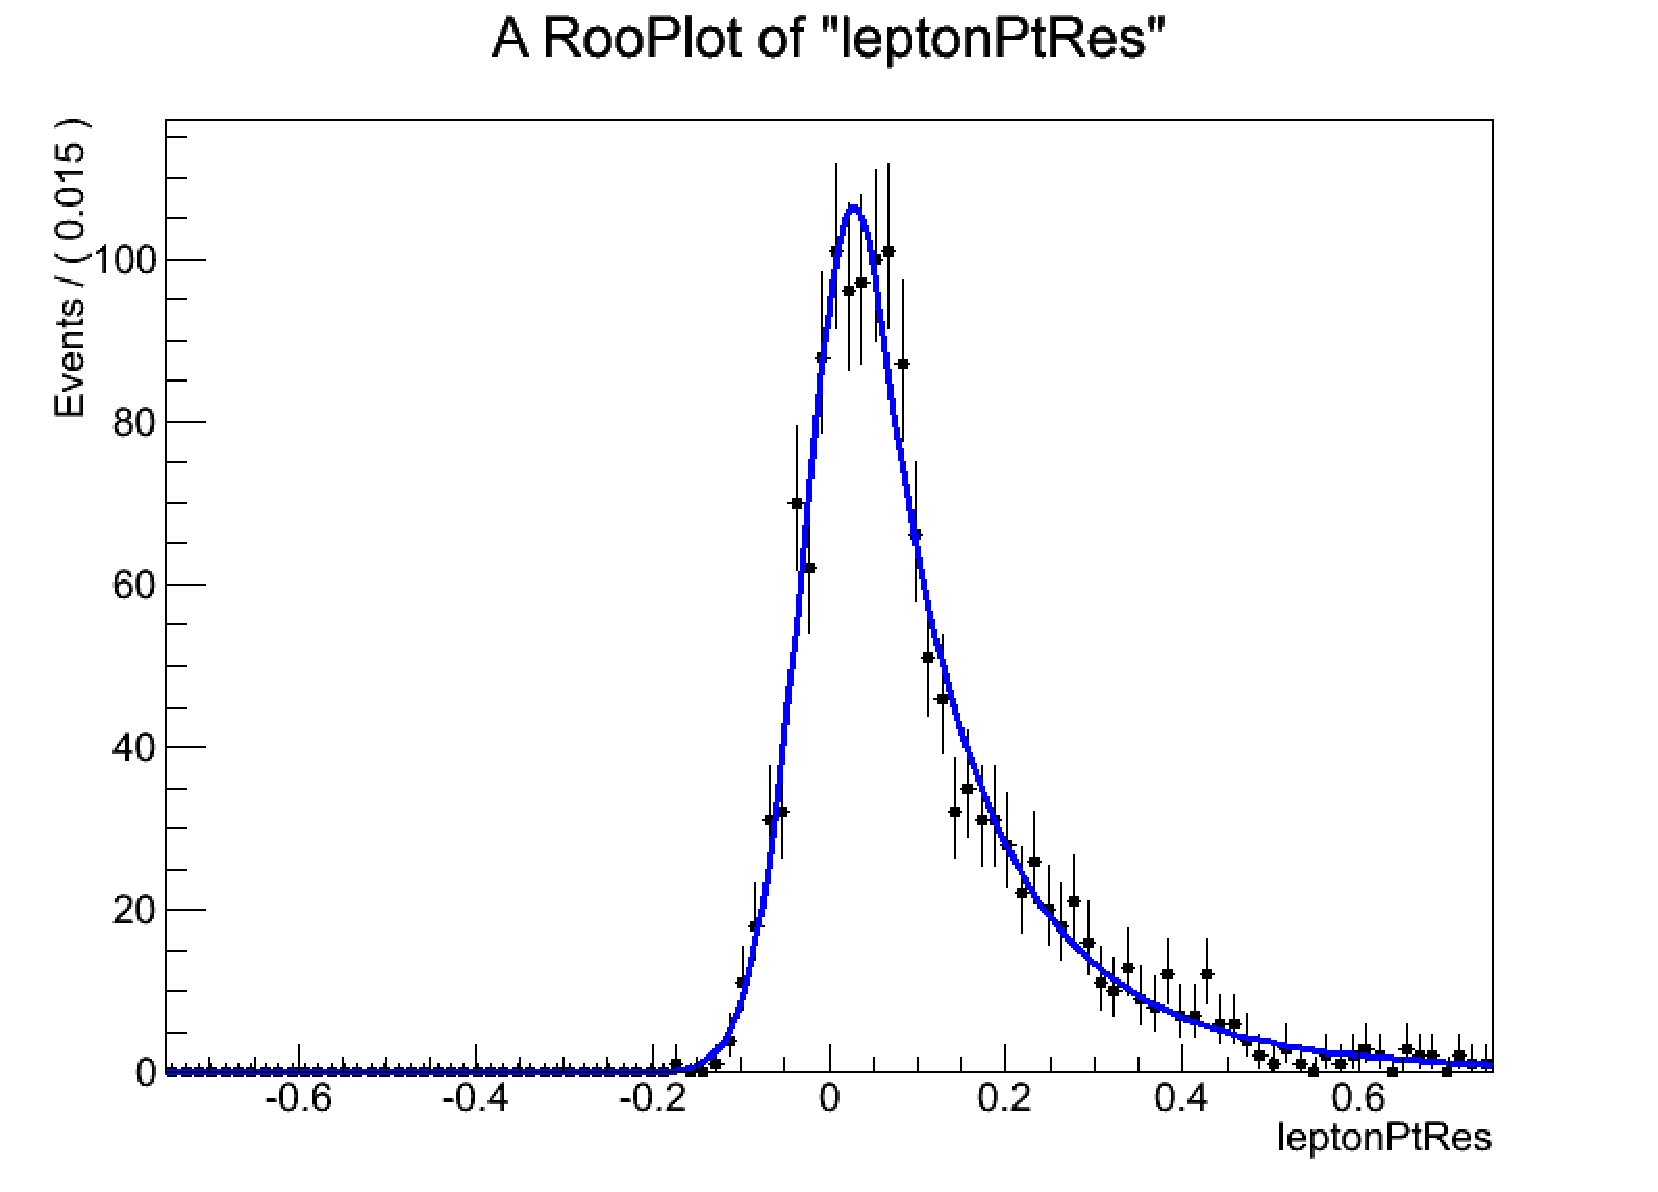
\includegraphics[width=0.245\textwidth]{figures/LeptonPtResolution_Electrons_PtBin2_EtaBin10.pdf}}
    \subfigure[$2.0 \le |\eta| < 2.1$]{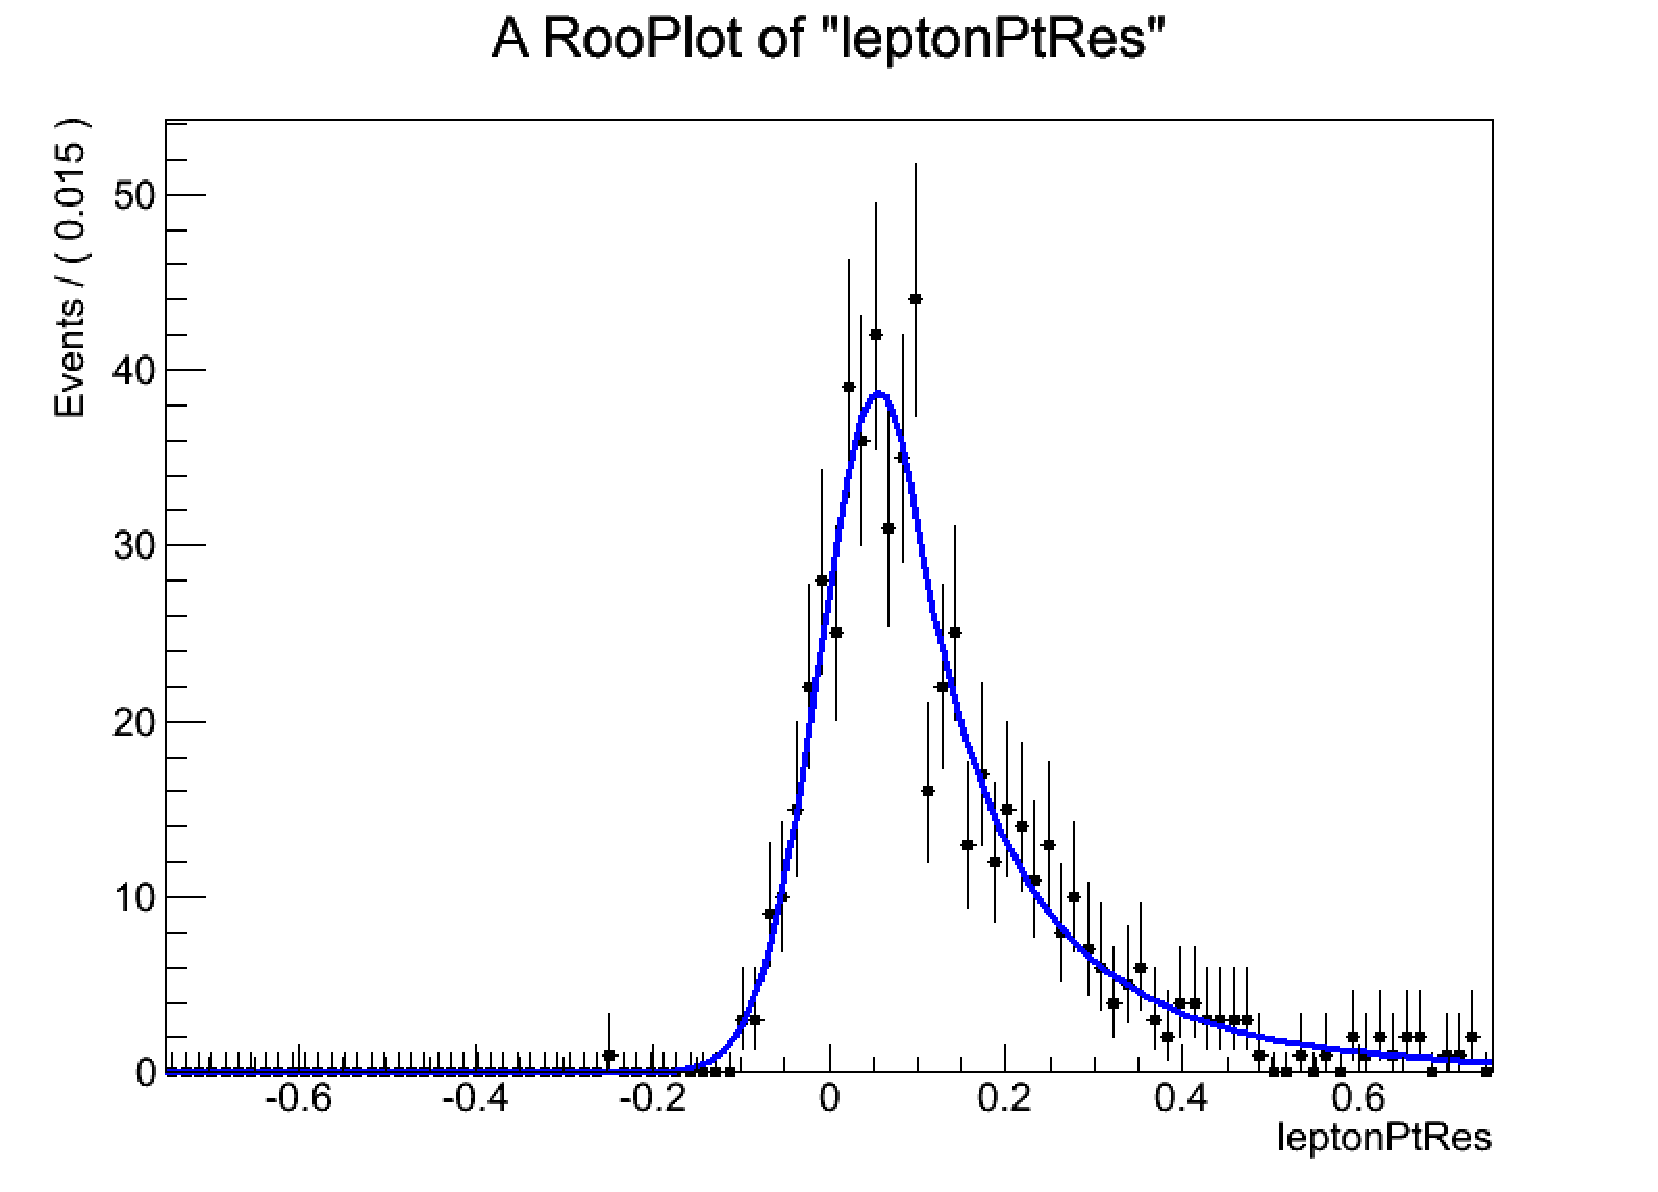
\includegraphics[width=0.245\textwidth]{figures/LeptonPtResolution_Electrons_PtBin2_EtaBin11.pdf}}
    \subfigure[$2.1 \le |\eta| < 2.2$]{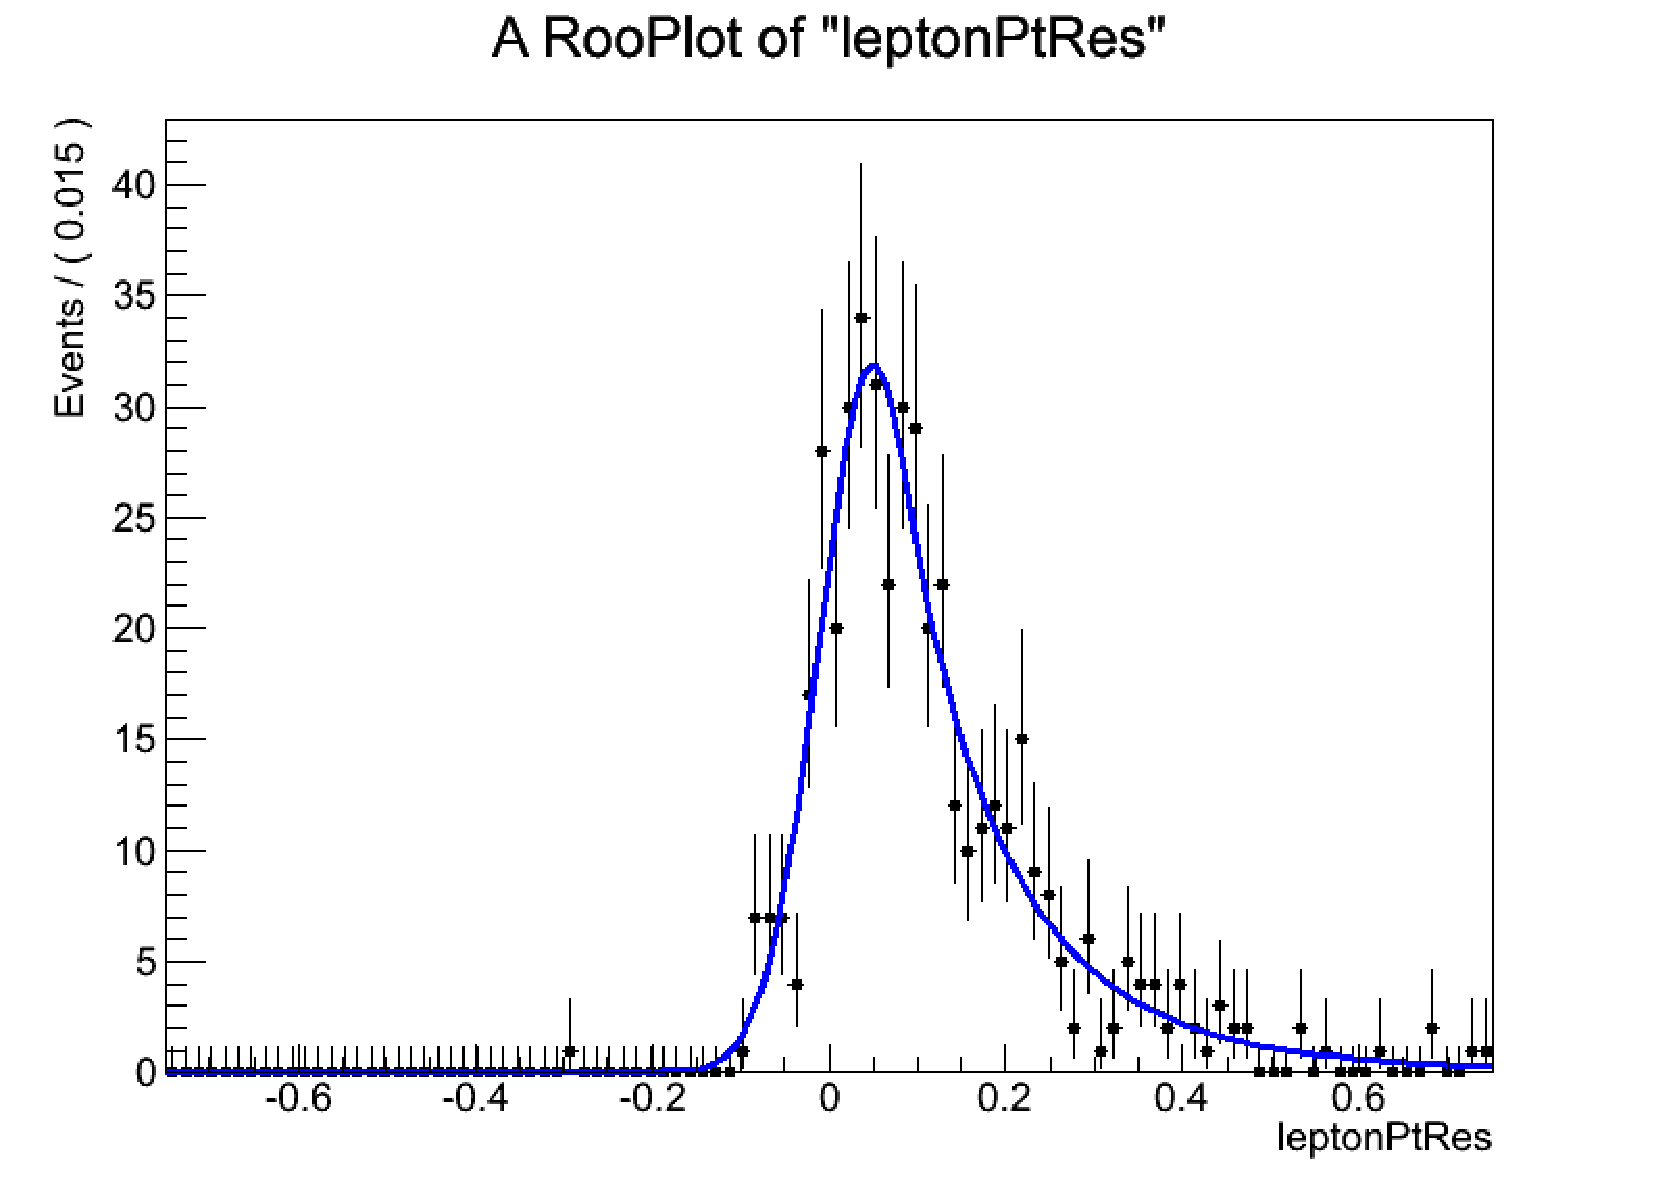
\includegraphics[width=0.245\textwidth]{figures/LeptonPtResolution_Electrons_PtBin2_EtaBin12.pdf}}
    \subfigure[$2.2 \le |\eta| < 2.3$]{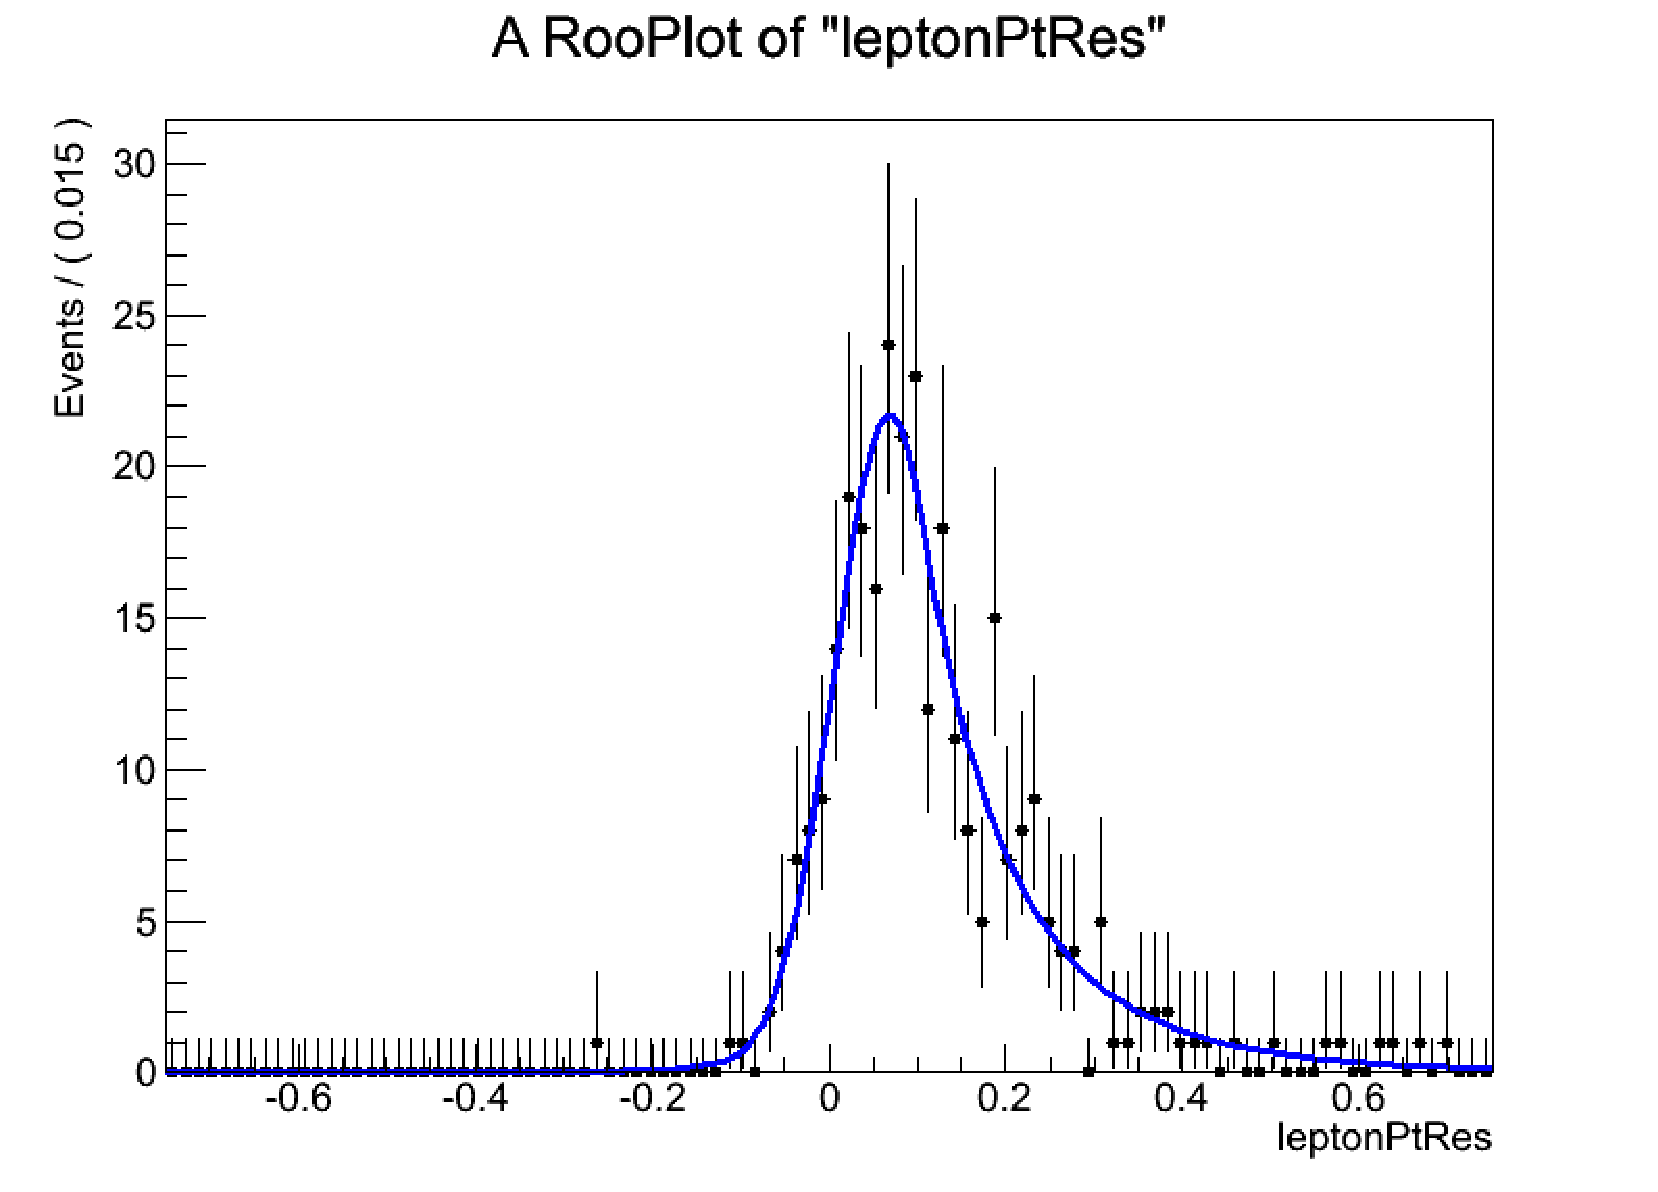
\includegraphics[width=0.245\textwidth]{figures/LeptonPtResolution_Electrons_PtBin2_EtaBin13.pdf}}
    \subfigure[$2.3 \le |\eta| < 2.4$]{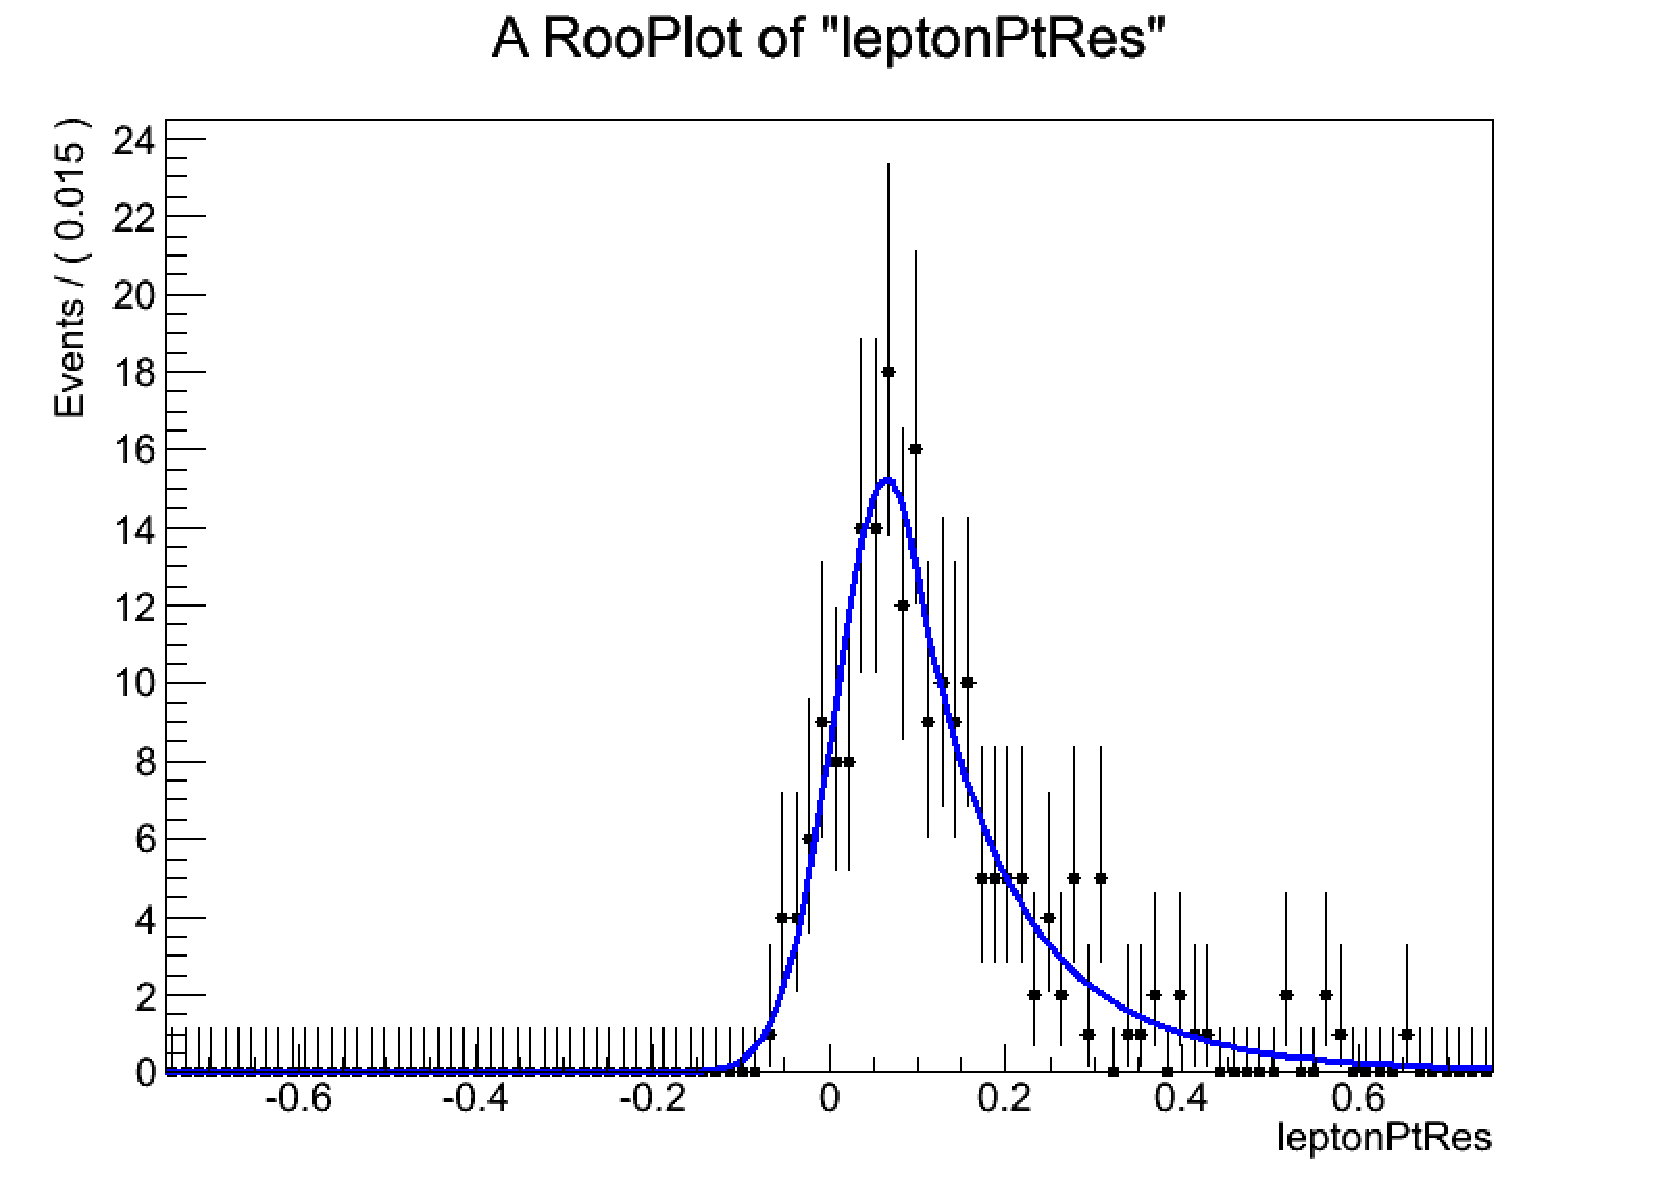
\includegraphics[width=0.245\textwidth]{figures/LeptonPtResolution_Electrons_PtBin2_EtaBin14.pdf}}
    \subfigure[$2.4 \le |\eta| < 2.5$]{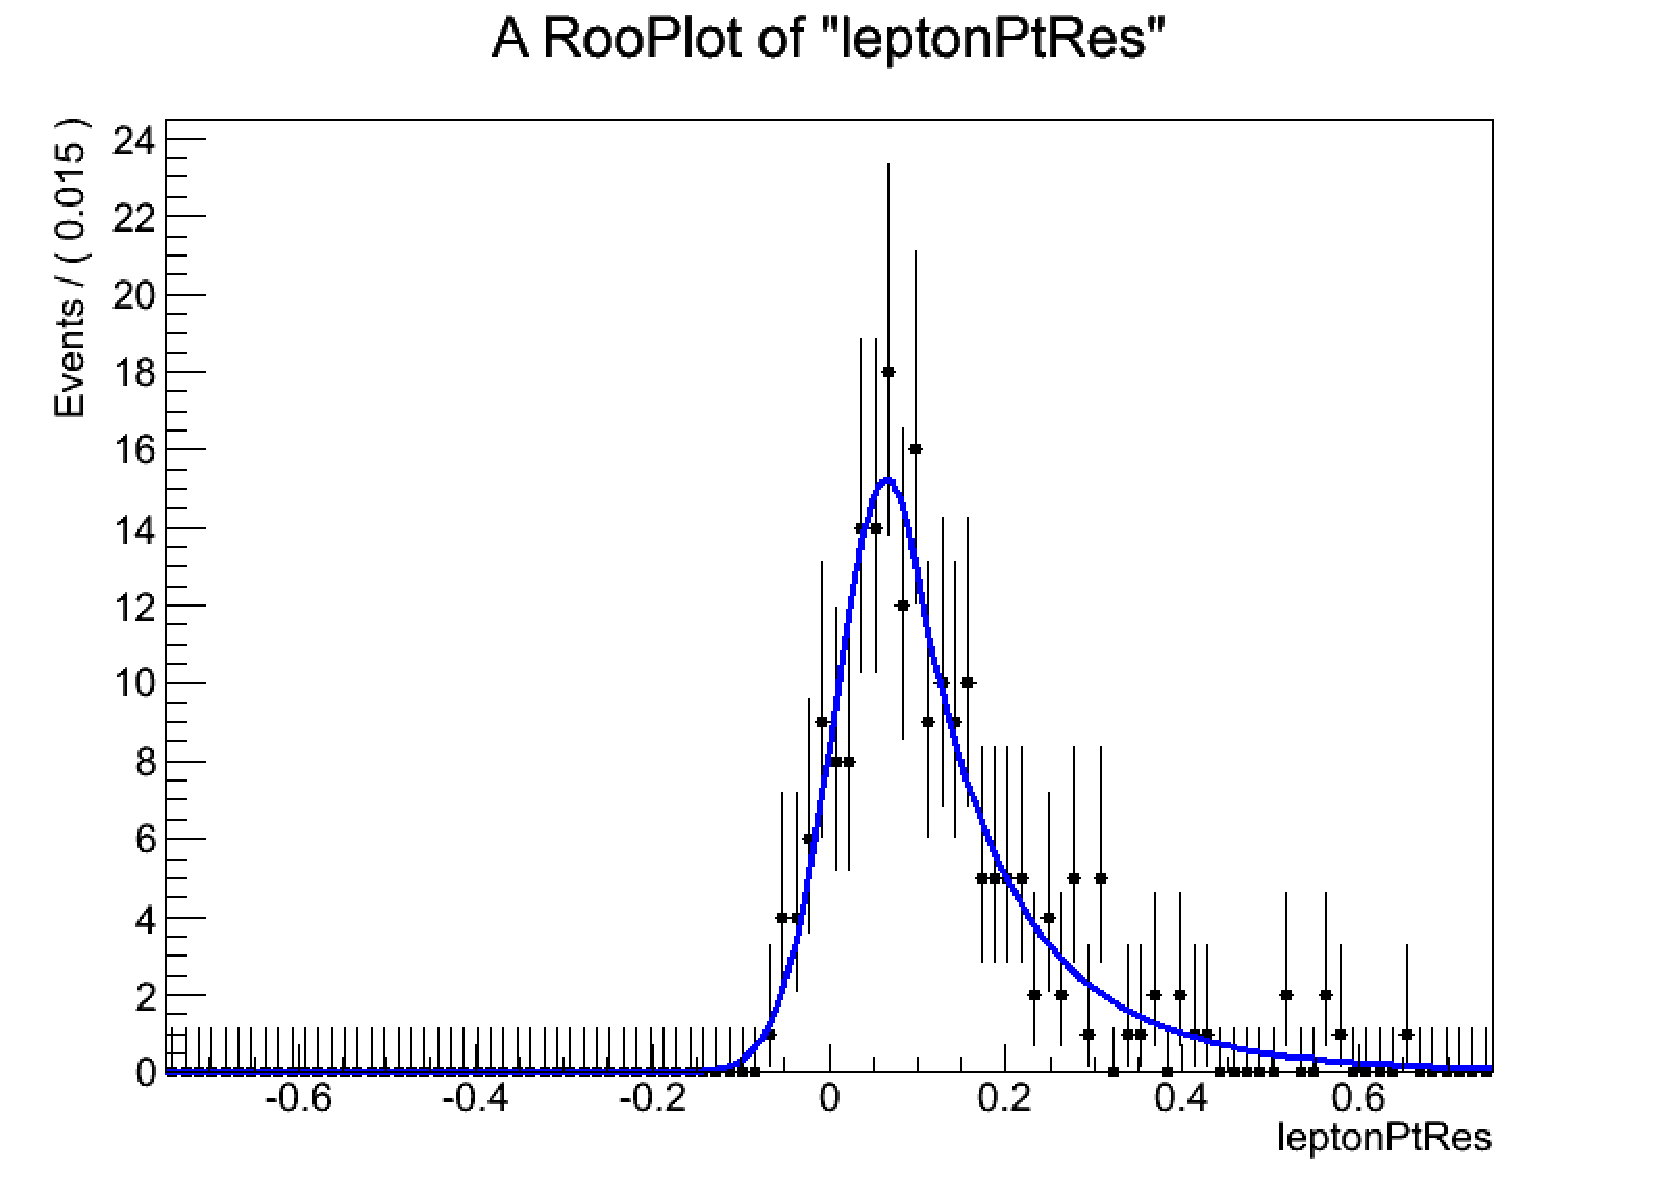
\includegraphics[width=0.245\textwidth]{figures/LeptonPtResolution_Electrons_PtBin2_EtaBin14.pdf}}
    \caption{ Energy response histogram and fitted response function for endcap electrons with $p_{T}$ between 
      $7$~\GeV and $8$~\GeV 
    }
    \label{fig:ElectronResponse_PtBin2_Endcap}
  \end{center}
\end{figure}


\begin{figure}[htb!]
  \begin{center}
    \subfigure[$|\eta| < 0.2$]{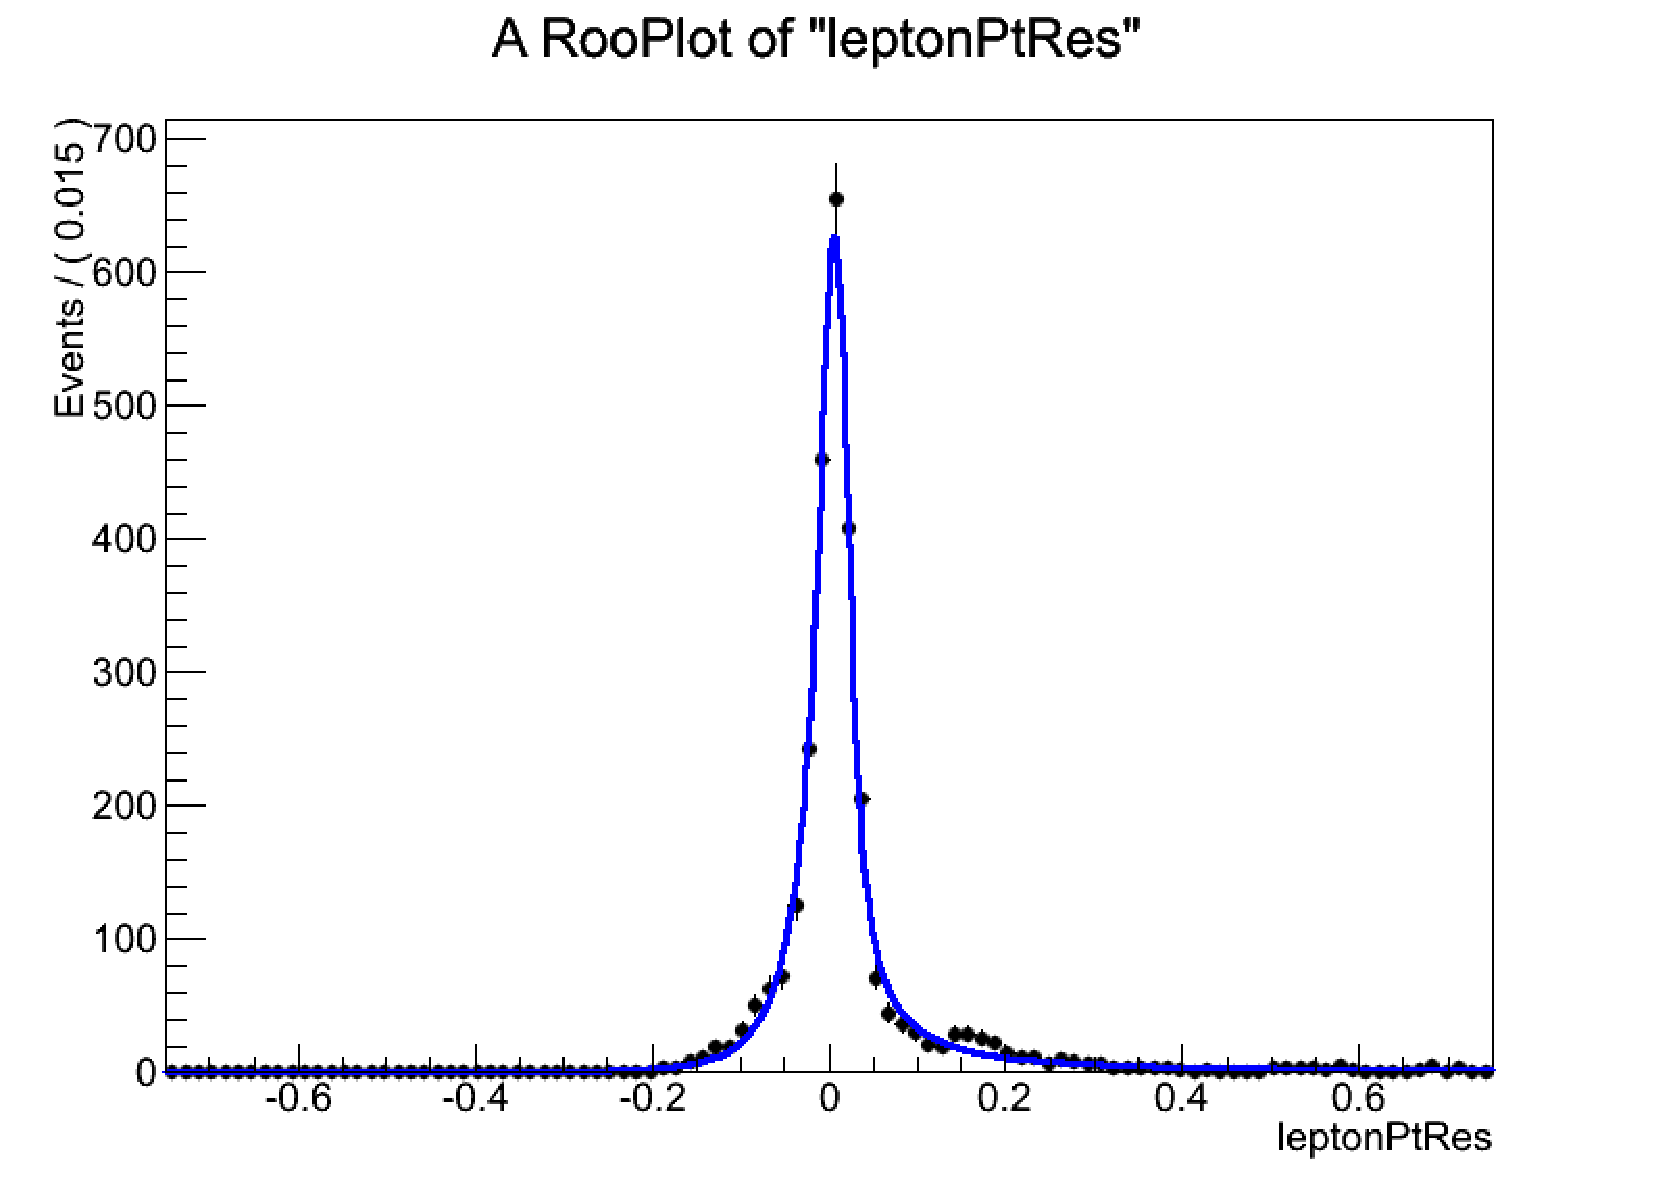
\includegraphics[width=0.245\textwidth]{figures/LeptonPtResolution_Electrons_PtBin3_EtaBin1.pdf}}
    \subfigure[$0.2 \le |\eta| < 0.4$]{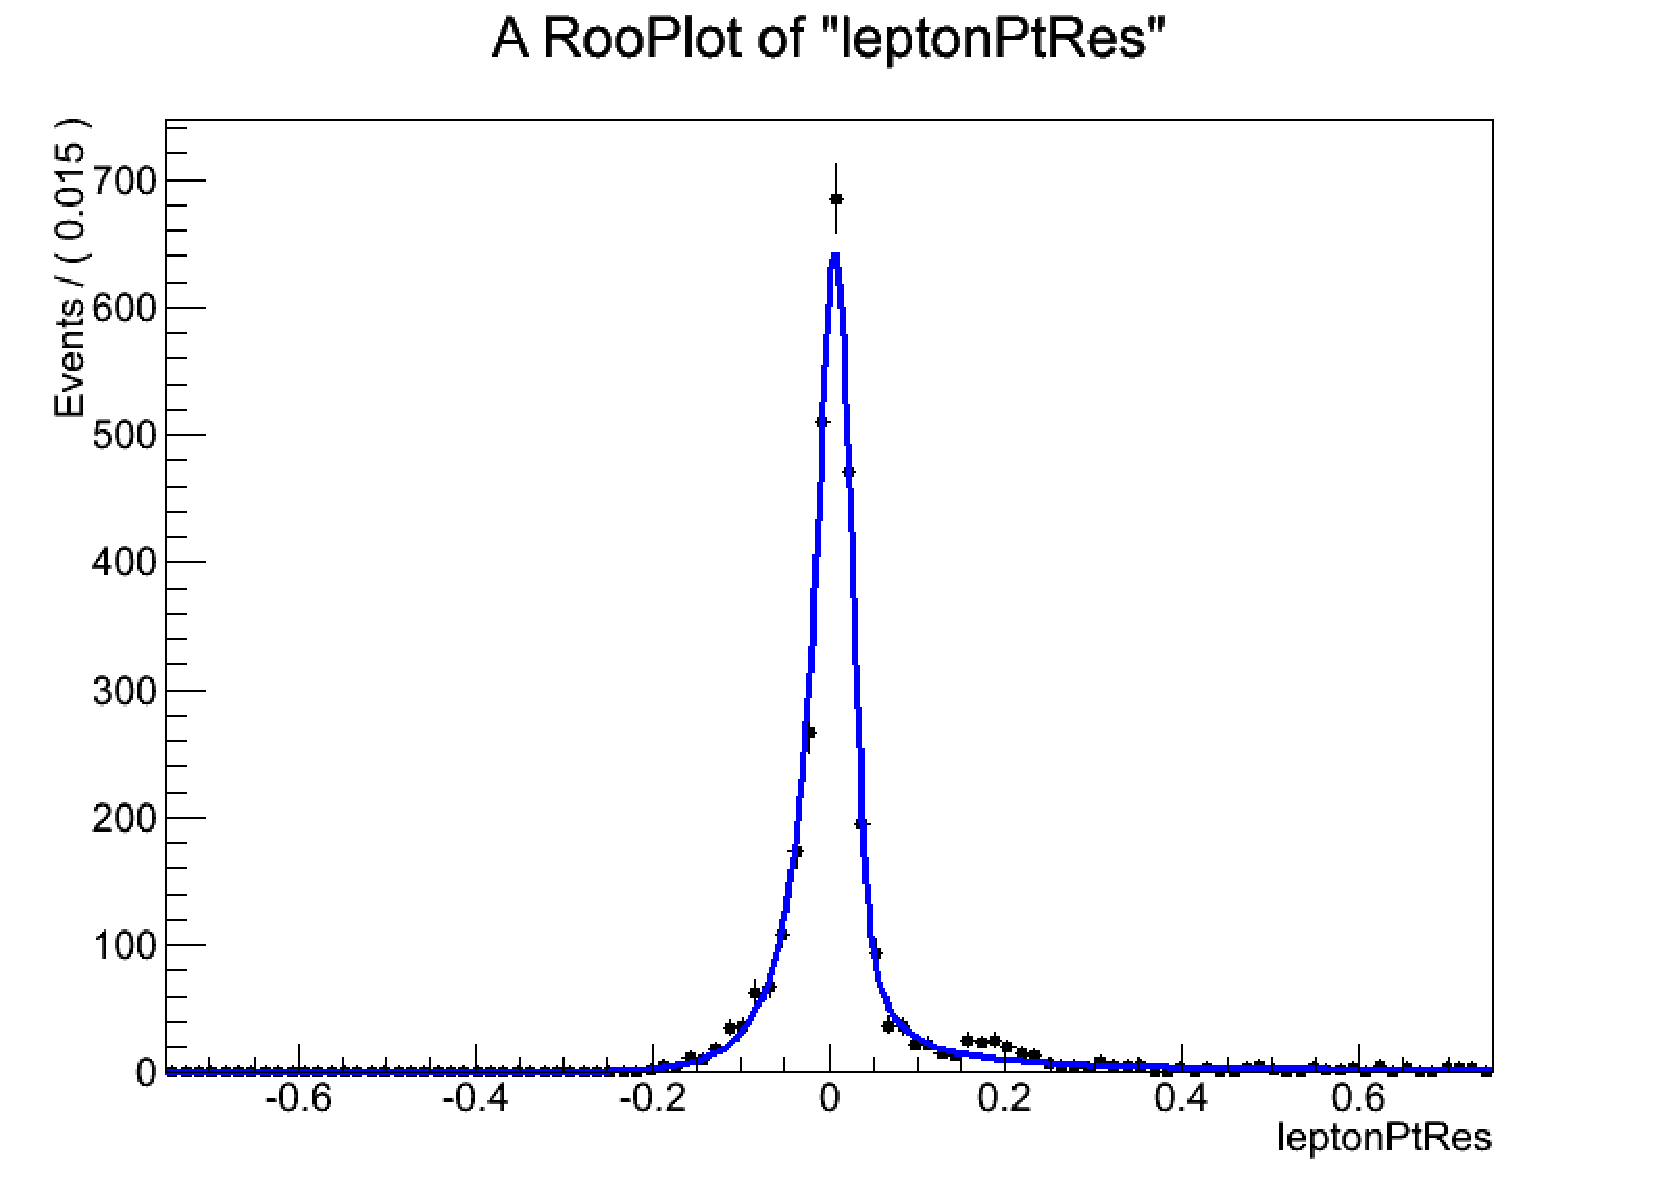
\includegraphics[width=0.245\textwidth]{figures/LeptonPtResolution_Electrons_PtBin3_EtaBin2.pdf}}
    \subfigure[$0.4 \le |\eta| < 0.6$]{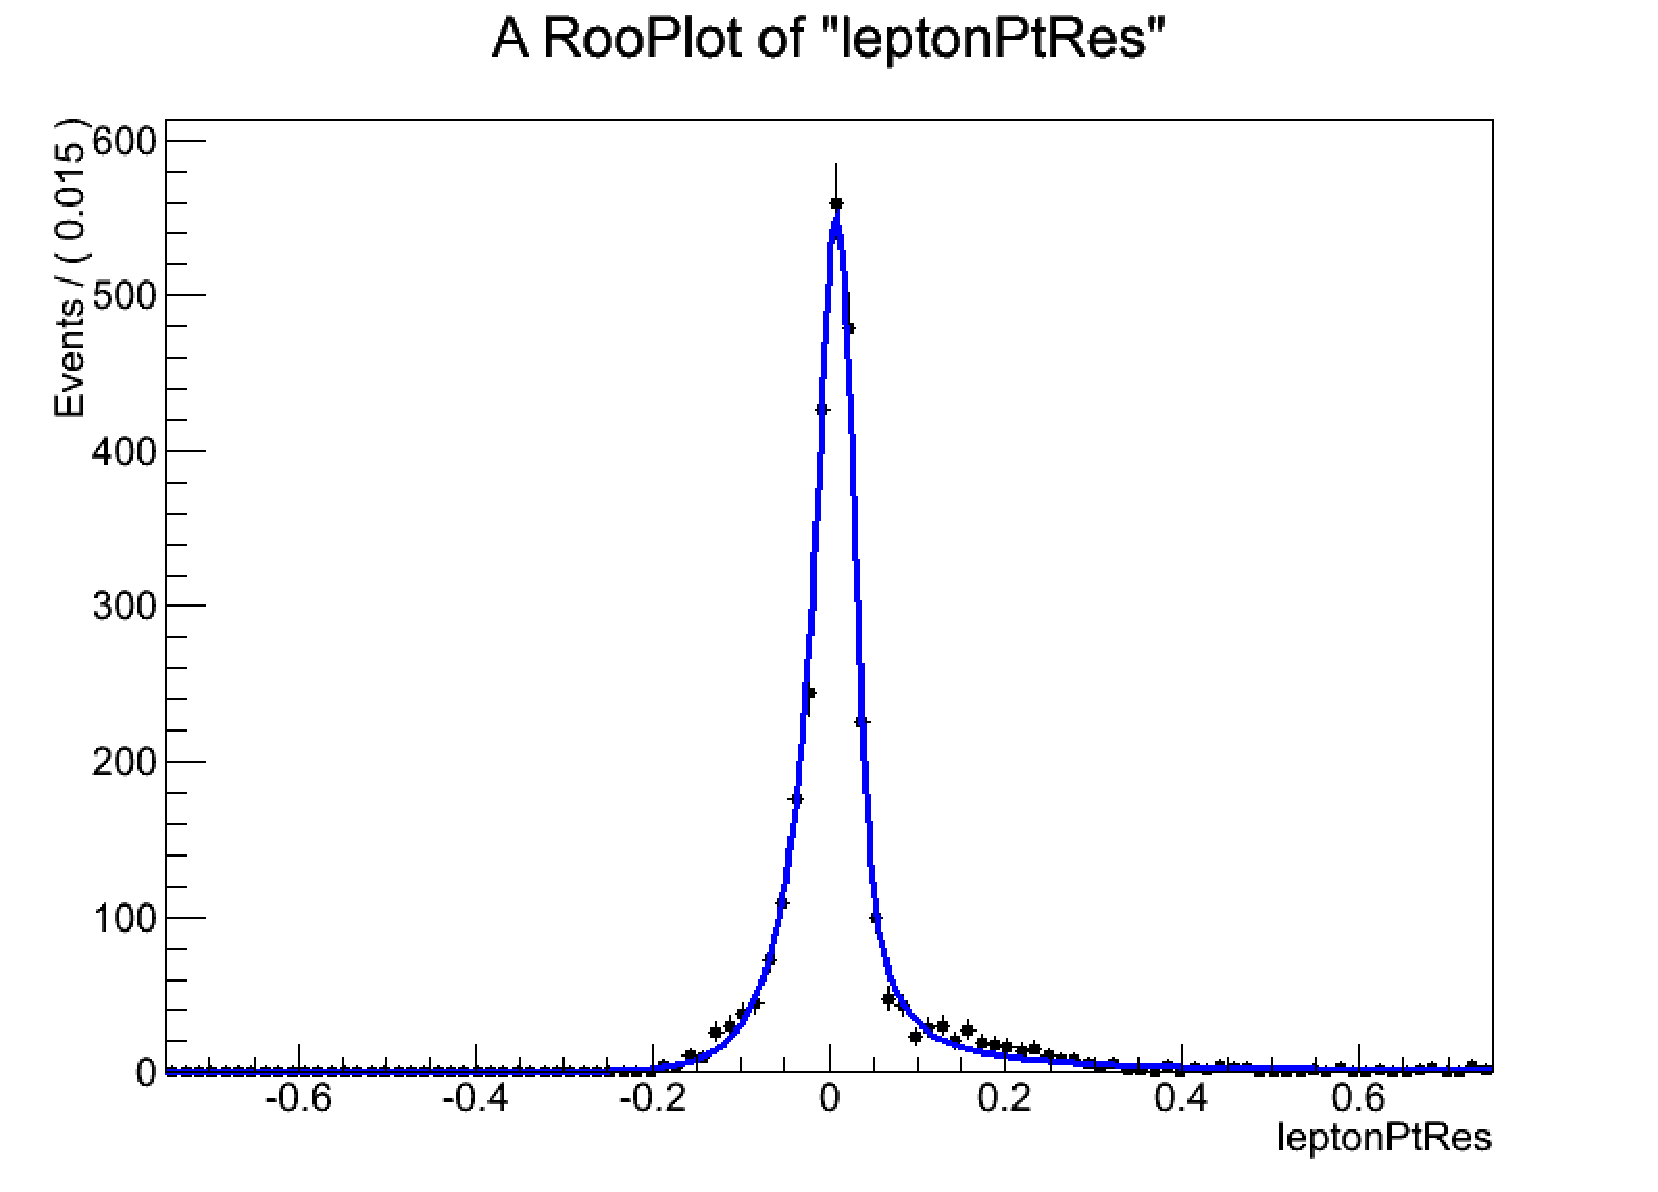
\includegraphics[width=0.245\textwidth]{figures/LeptonPtResolution_Electrons_PtBin3_EtaBin3.pdf}}
    \subfigure[$0.6 \le |\eta| < 0.8$]{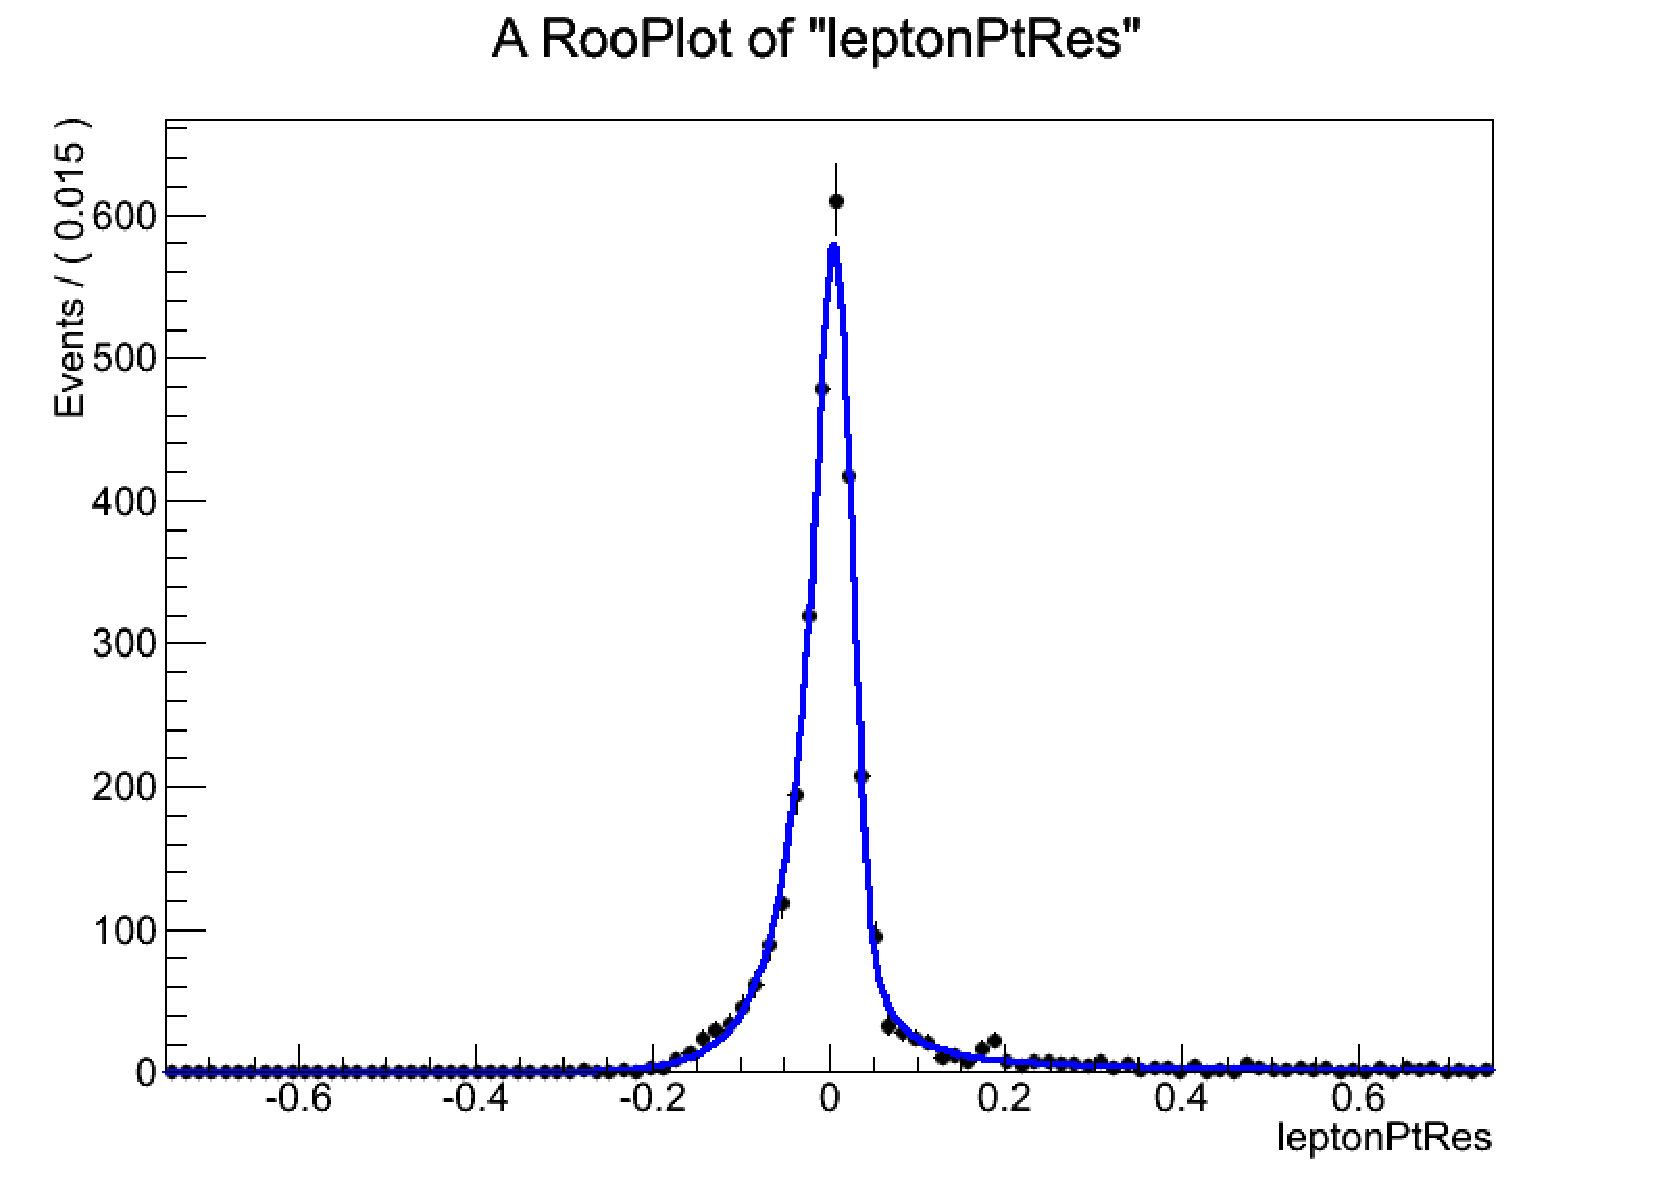
\includegraphics[width=0.245\textwidth]{figures/LeptonPtResolution_Electrons_PtBin3_EtaBin4.pdf}}
    \subfigure[$0.8 \le |\eta| < 1.0$]{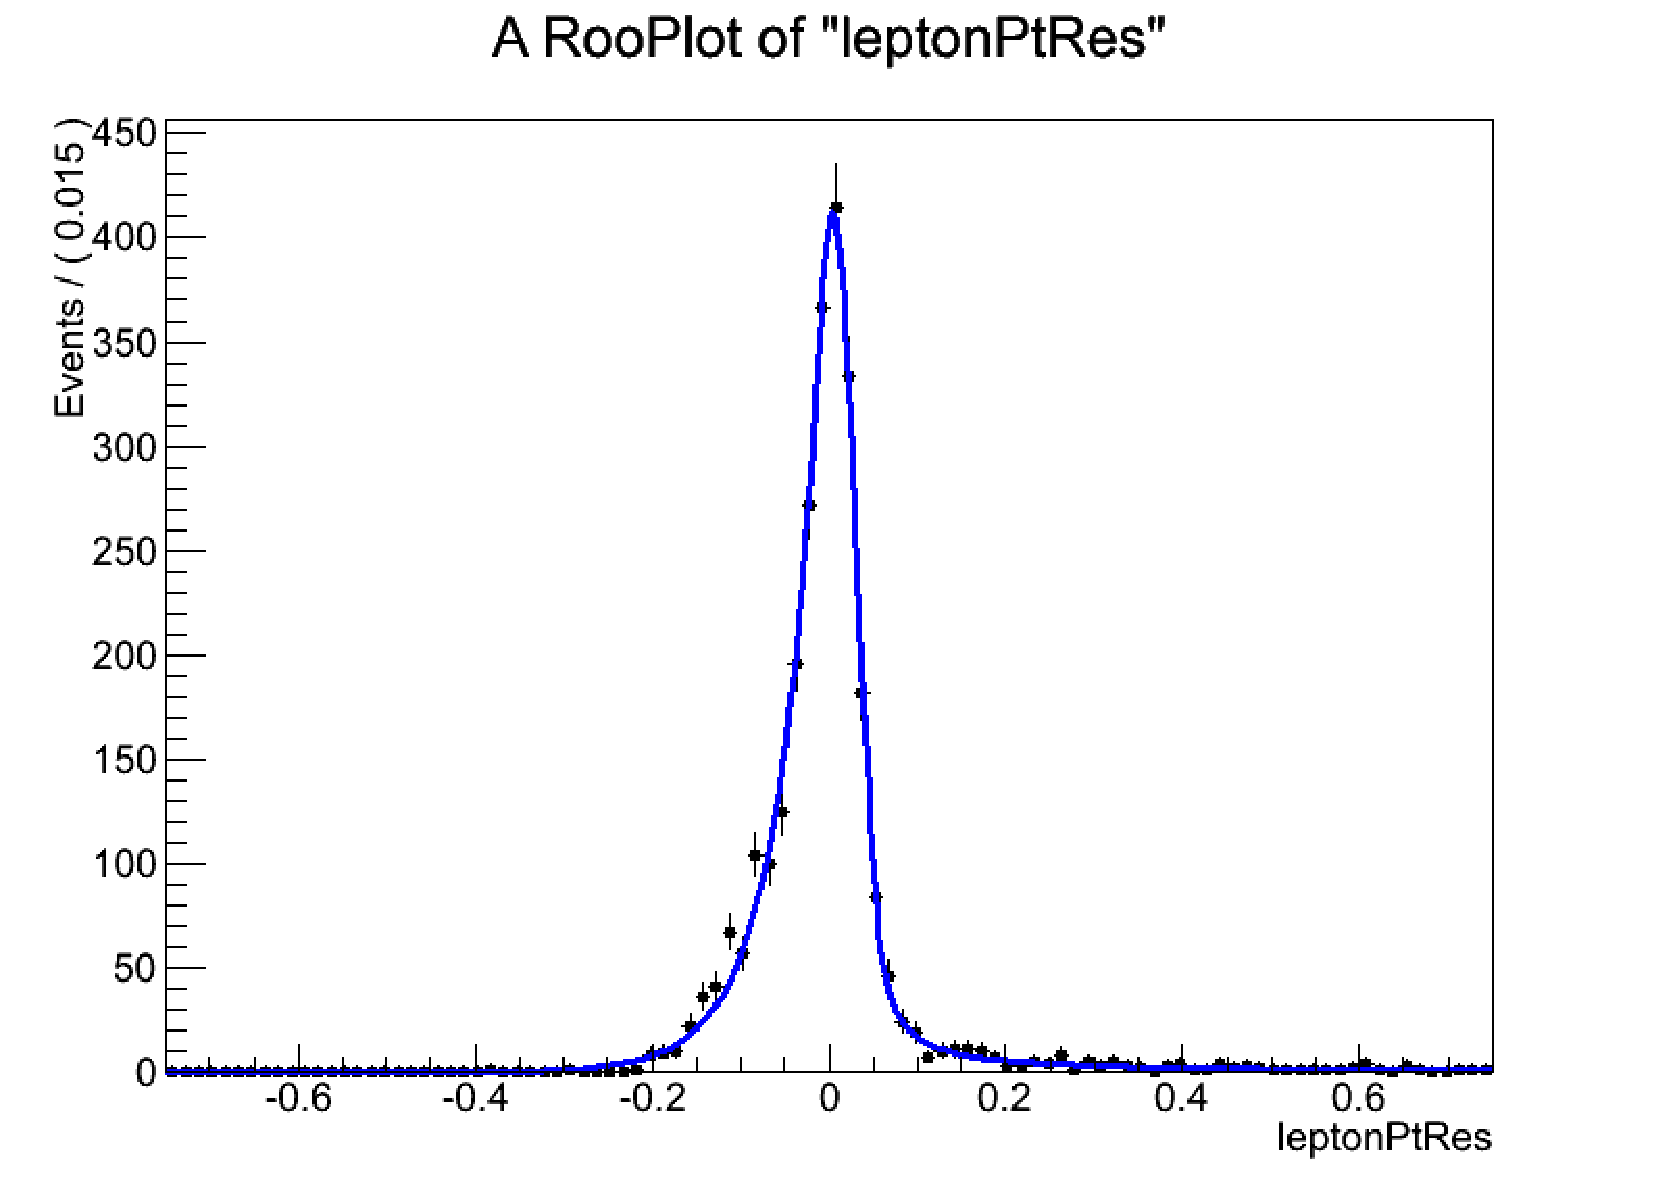
\includegraphics[width=0.245\textwidth]{figures/LeptonPtResolution_Electrons_PtBin3_EtaBin5.pdf}}
    \subfigure[$1.0 \le |\eta| < 1.2$]{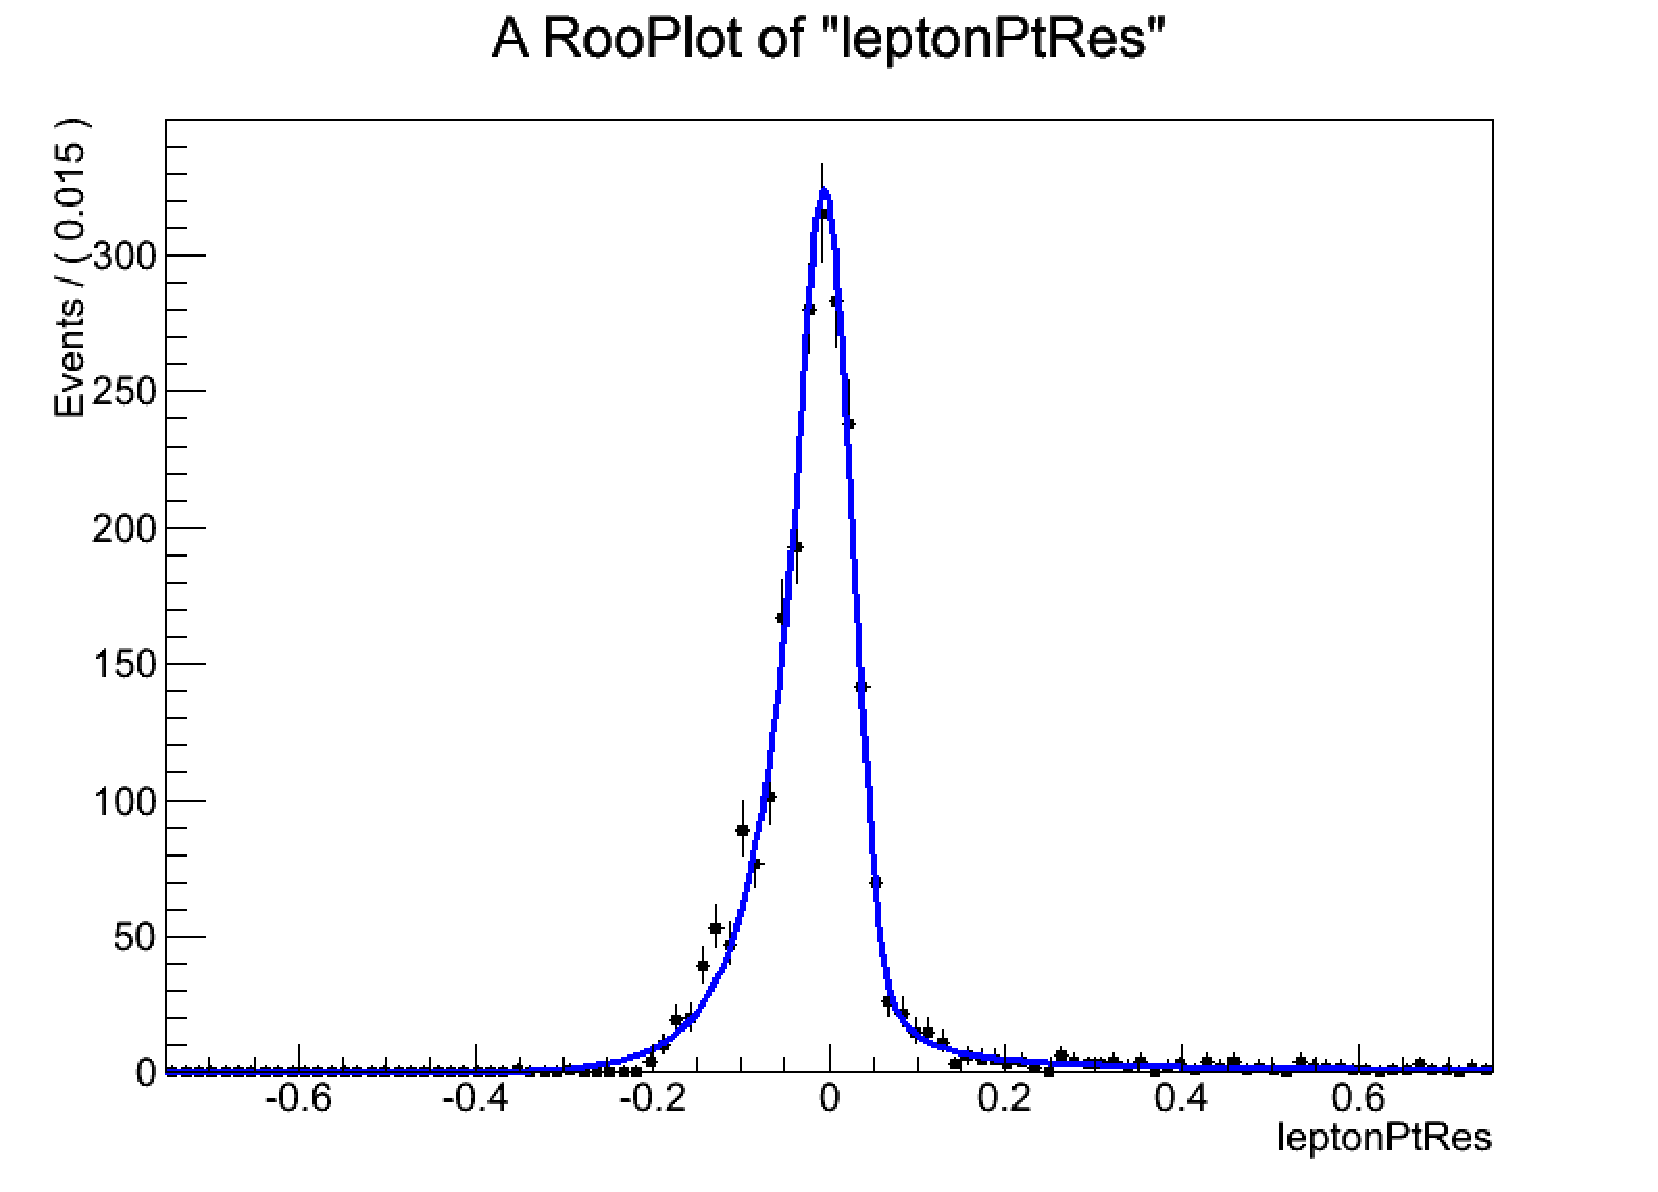
\includegraphics[width=0.245\textwidth]{figures/LeptonPtResolution_Electrons_PtBin3_EtaBin6.pdf}}
    \subfigure[$1.2 \le |\eta| < 1.4442$]{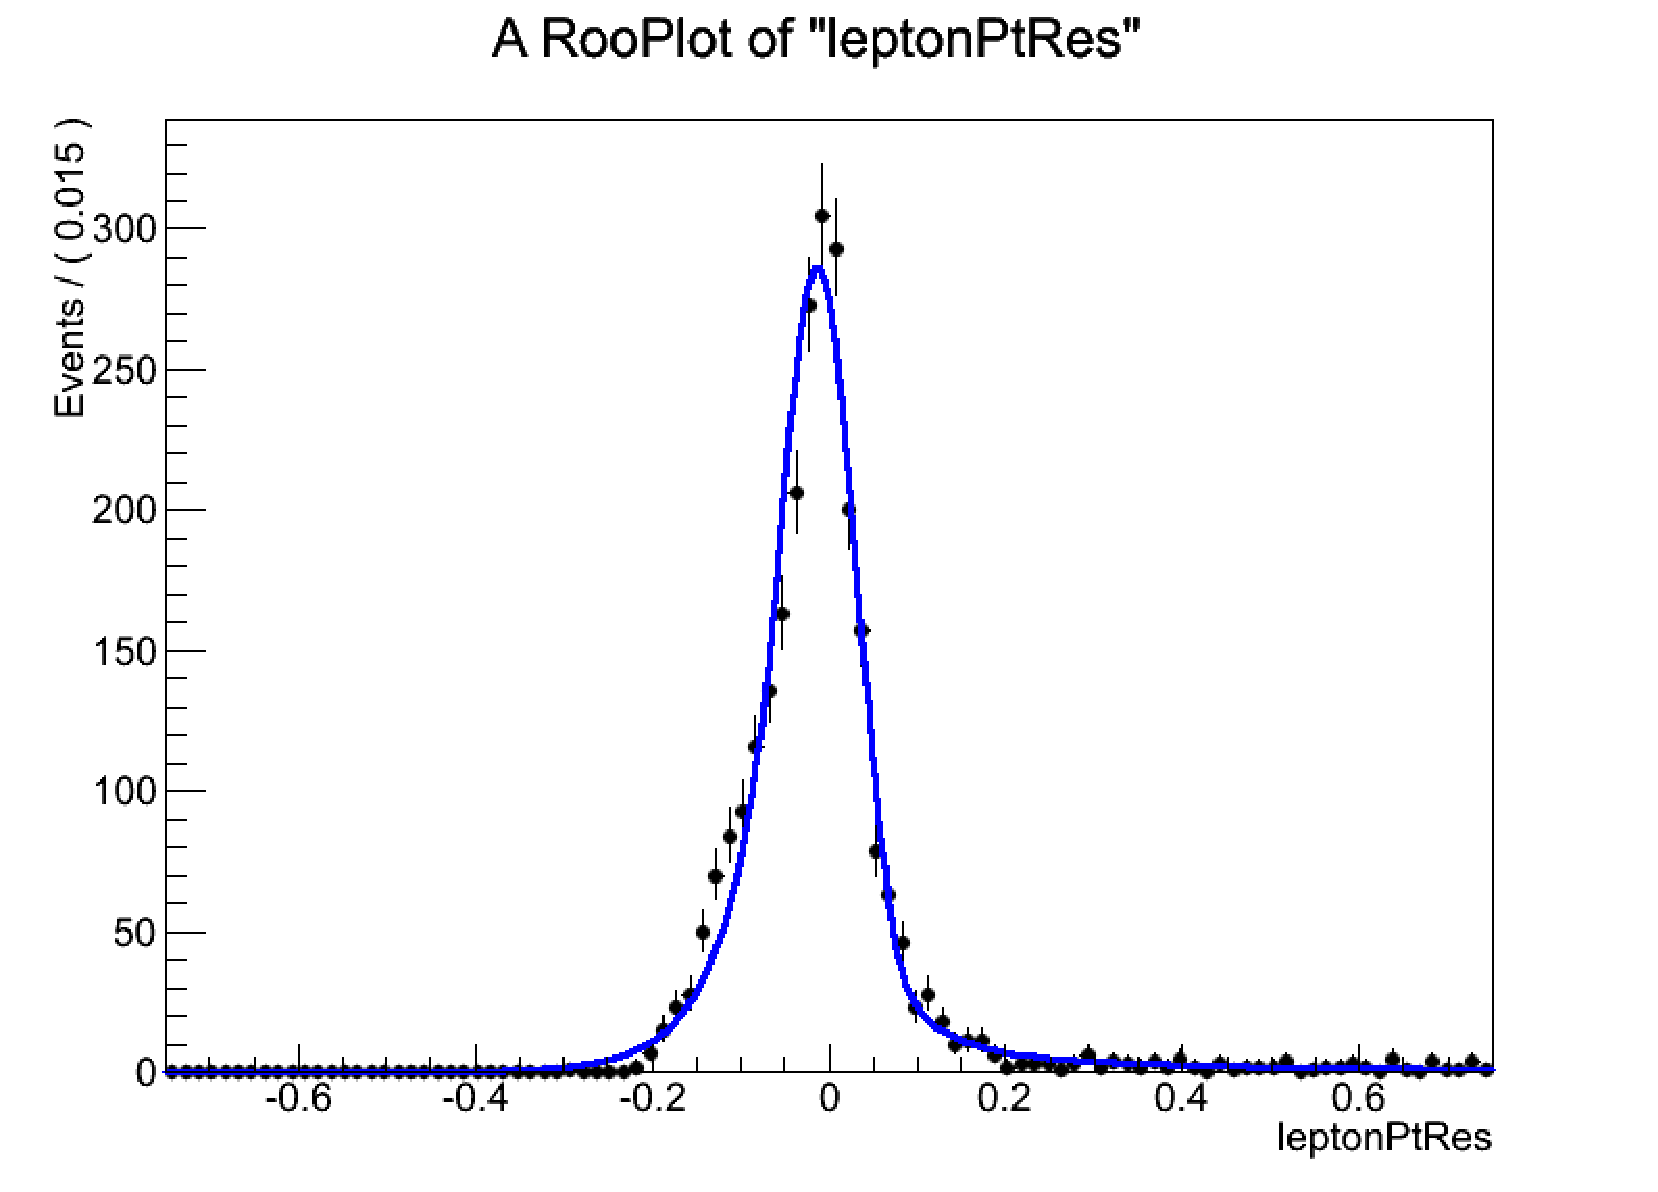
\includegraphics[width=0.245\textwidth]{figures/LeptonPtResolution_Electrons_PtBin3_EtaBin7.pdf}}
    \subfigure[$1.4 \le |\eta| < 1.566$]{\includegraphics[width=0.245\textwidth]{figures/LeptonPtResolution_Electrons_PtBin3_EtaBin8.pdf}}
    \caption{ Energy response histogram and fitted response function for barrel electrons with $p_{T}$ between 
      $8$~\GeV and $9$~\GeV 
    }
    \label{fig:ElectronResponse_PtBin3_Barrel}
  \end{center}
\end{figure}

\begin{figure}[htb!]
  \begin{center}
    \subfigure[$1.566 \le |\eta| < 1.8$]{\includegraphics[width=0.245\textwidth]{figures/LeptonPtResolution_Electrons_PtBin3_EtaBin9.pdf}}
    \subfigure[$1.8 \le |\eta| < 2.0$]{\includegraphics[width=0.245\textwidth]{figures/LeptonPtResolution_Electrons_PtBin3_EtaBin10.pdf}}
    \subfigure[$2.0 \le |\eta| < 2.1$]{\includegraphics[width=0.245\textwidth]{figures/LeptonPtResolution_Electrons_PtBin3_EtaBin11.pdf}}
    \subfigure[$2.1 \le |\eta| < 2.2$]{\includegraphics[width=0.245\textwidth]{figures/LeptonPtResolution_Electrons_PtBin3_EtaBin12.pdf}}
    \subfigure[$2.2 \le |\eta| < 2.3$]{\includegraphics[width=0.245\textwidth]{figures/LeptonPtResolution_Electrons_PtBin3_EtaBin13.pdf}}
    \subfigure[$2.3 \le |\eta| < 2.4$]{\includegraphics[width=0.245\textwidth]{figures/LeptonPtResolution_Electrons_PtBin3_EtaBin14.pdf}}
    \subfigure[$2.4 \le |\eta| < 2.5$]{\includegraphics[width=0.245\textwidth]{figures/LeptonPtResolution_Electrons_PtBin3_EtaBin14.pdf}}
    \caption{ Energy response histogram and fitted response function for endcap electrons with $p_{T}$ between 
      $8$~\GeV and $9$~\GeV 
    }
    \label{fig:ElectronResponse_PtBin3_Endcap}
  \end{center}
\end{figure}


\begin{figure}[htb!]
  \begin{center}
    \subfigure[$|\eta| < 0.2$]{\includegraphics[width=0.245\textwidth]{figures/LeptonPtResolution_Electrons_PtBin4_EtaBin1.pdf}}
    \subfigure[$0.2 \le |\eta| < 0.4$]{\includegraphics[width=0.245\textwidth]{figures/LeptonPtResolution_Electrons_PtBin4_EtaBin2.pdf}}
    \subfigure[$0.4 \le |\eta| < 0.6$]{\includegraphics[width=0.245\textwidth]{figures/LeptonPtResolution_Electrons_PtBin4_EtaBin3.pdf}}
    \subfigure[$0.6 \le |\eta| < 0.8$]{\includegraphics[width=0.245\textwidth]{figures/LeptonPtResolution_Electrons_PtBin4_EtaBin4.pdf}}
    \subfigure[$0.8 \le |\eta| < 1.0$]{\includegraphics[width=0.245\textwidth]{figures/LeptonPtResolution_Electrons_PtBin4_EtaBin5.pdf}}
    \subfigure[$1.0 \le |\eta| < 1.2$]{\includegraphics[width=0.245\textwidth]{figures/LeptonPtResolution_Electrons_PtBin4_EtaBin6.pdf}}
    \subfigure[$1.2 \le |\eta| < 1.4442$]{\includegraphics[width=0.245\textwidth]{figures/LeptonPtResolution_Electrons_PtBin4_EtaBin7.pdf}}
    \subfigure[$1.4 \le |\eta| < 1.566$]{\includegraphics[width=0.245\textwidth]{figures/LeptonPtResolution_Electrons_PtBin4_EtaBin8.pdf}}
    \caption{ Energy response histogram and fitted response function for barrel electrons with $p_{T}$ between 
      $9$~\GeV and $10$~\GeV 
    }
    \label{fig:ElectronResponse_PtBin4_Barrel}
  \end{center}
\end{figure}

\begin{figure}[htb!]
  \begin{center}
    \subfigure[$1.566 \le |\eta| < 1.8$]{\includegraphics[width=0.245\textwidth]{figures/LeptonPtResolution_Electrons_PtBin4_EtaBin9.pdf}}
    \subfigure[$1.8 \le |\eta| < 2.0$]{\includegraphics[width=0.245\textwidth]{figures/LeptonPtResolution_Electrons_PtBin4_EtaBin10.pdf}}
    \subfigure[$2.0 \le |\eta| < 2.1$]{\includegraphics[width=0.245\textwidth]{figures/LeptonPtResolution_Electrons_PtBin4_EtaBin11.pdf}}
    \subfigure[$2.1 \le |\eta| < 2.2$]{\includegraphics[width=0.245\textwidth]{figures/LeptonPtResolution_Electrons_PtBin4_EtaBin12.pdf}}
    \subfigure[$2.2 \le |\eta| < 2.3$]{\includegraphics[width=0.245\textwidth]{figures/LeptonPtResolution_Electrons_PtBin4_EtaBin13.pdf}}
    \subfigure[$2.3 \le |\eta| < 2.4$]{\includegraphics[width=0.245\textwidth]{figures/LeptonPtResolution_Electrons_PtBin4_EtaBin14.pdf}}
    \subfigure[$2.4 \le |\eta| < 2.5$]{\includegraphics[width=0.245\textwidth]{figures/LeptonPtResolution_Electrons_PtBin4_EtaBin14.pdf}}
    \caption{ Energy response histogram and fitted response function for endcap electrons with $p_{T}$ between 
      $9$~\GeV and $10$~\GeV 
    }
    \label{fig:ElectronResponse_PtBin4_Endcap}
  \end{center}
\end{figure}


\begin{figure}[htb!]
  \begin{center}
    \subfigure[$|\eta| < 0.2$]{\includegraphics[width=0.245\textwidth]{figures/LeptonPtResolution_Electrons_PtBin5_EtaBin1.pdf}}
    \subfigure[$0.2 \le |\eta| < 0.4$]{\includegraphics[width=0.245\textwidth]{figures/LeptonPtResolution_Electrons_PtBin5_EtaBin2.pdf}}
    \subfigure[$0.4 \le |\eta| < 0.6$]{\includegraphics[width=0.245\textwidth]{figures/LeptonPtResolution_Electrons_PtBin5_EtaBin3.pdf}}
    \subfigure[$0.6 \le |\eta| < 0.8$]{\includegraphics[width=0.245\textwidth]{figures/LeptonPtResolution_Electrons_PtBin5_EtaBin4.pdf}}
    \subfigure[$0.8 \le |\eta| < 1.0$]{\includegraphics[width=0.245\textwidth]{figures/LeptonPtResolution_Electrons_PtBin5_EtaBin5.pdf}}
    \subfigure[$1.0 \le |\eta| < 1.2$]{\includegraphics[width=0.245\textwidth]{figures/LeptonPtResolution_Electrons_PtBin5_EtaBin6.pdf}}
    \subfigure[$1.2 \le |\eta| < 1.4442$]{\includegraphics[width=0.245\textwidth]{figures/LeptonPtResolution_Electrons_PtBin5_EtaBin7.pdf}}
    \subfigure[$1.4 \le |\eta| < 1.566$]{\includegraphics[width=0.245\textwidth]{figures/LeptonPtResolution_Electrons_PtBin5_EtaBin8.pdf}}
    \caption{ Energy response histogram and fitted response function for barrel electrons with $p_{T}$ between 
      $10$~\GeV and $12$~\GeV 
    }
    \label{fig:ElectronResponse_PtBin5_Barrel}
  \end{center}
\end{figure}

\begin{figure}[htb!]
  \begin{center}
    \subfigure[$1.566 \le |\eta| < 1.8$]{\includegraphics[width=0.245\textwidth]{figures/LeptonPtResolution_Electrons_PtBin5_EtaBin9.pdf}}
    \subfigure[$1.8 \le |\eta| < 2.0$]{\includegraphics[width=0.245\textwidth]{figures/LeptonPtResolution_Electrons_PtBin5_EtaBin10.pdf}}
    \subfigure[$2.0 \le |\eta| < 2.1$]{\includegraphics[width=0.245\textwidth]{figures/LeptonPtResolution_Electrons_PtBin5_EtaBin11.pdf}}
    \subfigure[$2.1 \le |\eta| < 2.2$]{\includegraphics[width=0.245\textwidth]{figures/LeptonPtResolution_Electrons_PtBin5_EtaBin12.pdf}}
    \subfigure[$2.2 \le |\eta| < 2.3$]{\includegraphics[width=0.245\textwidth]{figures/LeptonPtResolution_Electrons_PtBin5_EtaBin13.pdf}}
    \subfigure[$2.3 \le |\eta| < 2.4$]{\includegraphics[width=0.245\textwidth]{figures/LeptonPtResolution_Electrons_PtBin5_EtaBin14.pdf}}
    \subfigure[$2.4 \le |\eta| < 2.5$]{\includegraphics[width=0.245\textwidth]{figures/LeptonPtResolution_Electrons_PtBin5_EtaBin14.pdf}}
    \caption{ Energy response histogram and fitted response function for endcap electrons with $p_{T}$ between 
      $10$~\GeV and $12$~\GeV 
    }
    \label{fig:ElectronResponse_PtBin5_Endcap}
  \end{center}
\end{figure}


\begin{figure}[htb!]
  \begin{center}
    \subfigure[$|\eta| < 0.2$]{\includegraphics[width=0.245\textwidth]{figures/LeptonPtResolution_Electrons_PtBin6_EtaBin1.pdf}}
    \subfigure[$0.2 \le |\eta| < 0.4$]{\includegraphics[width=0.245\textwidth]{figures/LeptonPtResolution_Electrons_PtBin6_EtaBin2.pdf}}
    \subfigure[$0.4 \le |\eta| < 0.6$]{\includegraphics[width=0.245\textwidth]{figures/LeptonPtResolution_Electrons_PtBin6_EtaBin3.pdf}}
    \subfigure[$0.6 \le |\eta| < 0.8$]{\includegraphics[width=0.245\textwidth]{figures/LeptonPtResolution_Electrons_PtBin6_EtaBin4.pdf}}
    \subfigure[$0.8 \le |\eta| < 1.0$]{\includegraphics[width=0.245\textwidth]{figures/LeptonPtResolution_Electrons_PtBin6_EtaBin5.pdf}}
    \subfigure[$1.0 \le |\eta| < 1.2$]{\includegraphics[width=0.245\textwidth]{figures/LeptonPtResolution_Electrons_PtBin6_EtaBin6.pdf}}
    \subfigure[$1.2 \le |\eta| < 1.4442$]{\includegraphics[width=0.245\textwidth]{figures/LeptonPtResolution_Electrons_PtBin6_EtaBin7.pdf}}
    \subfigure[$1.4 \le |\eta| < 1.566$]{\includegraphics[width=0.245\textwidth]{figures/LeptonPtResolution_Electrons_PtBin6_EtaBin8.pdf}}
    \caption{ Energy response histogram and fitted response function for barrel electrons with $p_{T}$ between 
      $12$~\GeV and $14$~\GeV 
    }
    \label{fig:ElectronResponse_PtBin6_Barrel}
  \end{center}
\end{figure}

\begin{figure}[htb!]
  \begin{center}
    \subfigure[$1.566 \le |\eta| < 1.8$]{\includegraphics[width=0.245\textwidth]{figures/LeptonPtResolution_Electrons_PtBin6_EtaBin9.pdf}}
    \subfigure[$1.8 \le |\eta| < 2.0$]{\includegraphics[width=0.245\textwidth]{figures/LeptonPtResolution_Electrons_PtBin6_EtaBin10.pdf}}
    \subfigure[$2.0 \le |\eta| < 2.1$]{\includegraphics[width=0.245\textwidth]{figures/LeptonPtResolution_Electrons_PtBin6_EtaBin11.pdf}}
    \subfigure[$2.1 \le |\eta| < 2.2$]{\includegraphics[width=0.245\textwidth]{figures/LeptonPtResolution_Electrons_PtBin6_EtaBin12.pdf}}
    \subfigure[$2.2 \le |\eta| < 2.3$]{\includegraphics[width=0.245\textwidth]{figures/LeptonPtResolution_Electrons_PtBin6_EtaBin13.pdf}}
    \subfigure[$2.3 \le |\eta| < 2.4$]{\includegraphics[width=0.245\textwidth]{figures/LeptonPtResolution_Electrons_PtBin6_EtaBin14.pdf}}
    \subfigure[$2.4 \le |\eta| < 2.5$]{\includegraphics[width=0.245\textwidth]{figures/LeptonPtResolution_Electrons_PtBin6_EtaBin14.pdf}}
    \caption{ Energy response histogram and fitted response function for endcap electrons with $p_{T}$ between 
      $12$~\GeV and $14$~\GeV 
    }
    \label{fig:ElectronResponse_PtBin6_Endcap}
  \end{center}
\end{figure}


\begin{figure}[htb!]
  \begin{center}
    \subfigure[$|\eta| < 0.2$]{\includegraphics[width=0.245\textwidth]{figures/LeptonPtResolution_Electrons_PtBin7_EtaBin1.pdf}}
    \subfigure[$0.2 \le |\eta| < 0.4$]{\includegraphics[width=0.245\textwidth]{figures/LeptonPtResolution_Electrons_PtBin7_EtaBin2.pdf}}
    \subfigure[$0.4 \le |\eta| < 0.6$]{\includegraphics[width=0.245\textwidth]{figures/LeptonPtResolution_Electrons_PtBin7_EtaBin3.pdf}}
    \subfigure[$0.6 \le |\eta| < 0.8$]{\includegraphics[width=0.245\textwidth]{figures/LeptonPtResolution_Electrons_PtBin7_EtaBin4.pdf}}
    \subfigure[$0.8 \le |\eta| < 1.0$]{\includegraphics[width=0.245\textwidth]{figures/LeptonPtResolution_Electrons_PtBin7_EtaBin5.pdf}}
    \subfigure[$1.0 \le |\eta| < 1.2$]{\includegraphics[width=0.245\textwidth]{figures/LeptonPtResolution_Electrons_PtBin7_EtaBin6.pdf}}
    \subfigure[$1.2 \le |\eta| < 1.4442$]{\includegraphics[width=0.245\textwidth]{figures/LeptonPtResolution_Electrons_PtBin7_EtaBin7.pdf}}
    \subfigure[$1.4 \le |\eta| < 1.566$]{\includegraphics[width=0.245\textwidth]{figures/LeptonPtResolution_Electrons_PtBin7_EtaBin8.pdf}}
    \caption{ Energy response histogram and fitted response function for barrel electrons with $p_{T}$ between 
      $14$~\GeV and $16$~\GeV 
    }
    \label{fig:ElectronResponse_PtBin7_Barrel}
  \end{center}
\end{figure}

\begin{figure}[htb!]
  \begin{center}
    \subfigure[$1.566 \le |\eta| < 1.8$]{\includegraphics[width=0.245\textwidth]{figures/LeptonPtResolution_Electrons_PtBin7_EtaBin9.pdf}}
    \subfigure[$1.8 \le |\eta| < 2.0$]{\includegraphics[width=0.245\textwidth]{figures/LeptonPtResolution_Electrons_PtBin7_EtaBin10.pdf}}
    \subfigure[$2.0 \le |\eta| < 2.1$]{\includegraphics[width=0.245\textwidth]{figures/LeptonPtResolution_Electrons_PtBin7_EtaBin11.pdf}}
    \subfigure[$2.1 \le |\eta| < 2.2$]{\includegraphics[width=0.245\textwidth]{figures/LeptonPtResolution_Electrons_PtBin7_EtaBin12.pdf}}
    \subfigure[$2.2 \le |\eta| < 2.3$]{\includegraphics[width=0.245\textwidth]{figures/LeptonPtResolution_Electrons_PtBin7_EtaBin13.pdf}}
    \subfigure[$2.3 \le |\eta| < 2.4$]{\includegraphics[width=0.245\textwidth]{figures/LeptonPtResolution_Electrons_PtBin7_EtaBin14.pdf}}
    \subfigure[$2.4 \le |\eta| < 2.5$]{\includegraphics[width=0.245\textwidth]{figures/LeptonPtResolution_Electrons_PtBin7_EtaBin14.pdf}}
    \caption{ Energy response histogram and fitted response function for endcap electrons with $p_{T}$ between 
      $14$~\GeV and $16$~\GeV 
    }
    \label{fig:ElectronResponse_PtBin7_Endcap}
  \end{center}
\end{figure}


\begin{figure}[htb!]
  \begin{center}
    \subfigure[$|\eta| < 0.2$]{\includegraphics[width=0.245\textwidth]{figures/LeptonPtResolution_Electrons_PtBin8_EtaBin1.pdf}}
    \subfigure[$0.2 \le |\eta| < 0.4$]{\includegraphics[width=0.245\textwidth]{figures/LeptonPtResolution_Electrons_PtBin8_EtaBin2.pdf}}
    \subfigure[$0.4 \le |\eta| < 0.6$]{\includegraphics[width=0.245\textwidth]{figures/LeptonPtResolution_Electrons_PtBin8_EtaBin3.pdf}}
    \subfigure[$0.6 \le |\eta| < 0.8$]{\includegraphics[width=0.245\textwidth]{figures/LeptonPtResolution_Electrons_PtBin8_EtaBin4.pdf}}
    \subfigure[$0.8 \le |\eta| < 1.0$]{\includegraphics[width=0.245\textwidth]{figures/LeptonPtResolution_Electrons_PtBin8_EtaBin5.pdf}}
    \subfigure[$1.0 \le |\eta| < 1.2$]{\includegraphics[width=0.245\textwidth]{figures/LeptonPtResolution_Electrons_PtBin8_EtaBin6.pdf}}
    \subfigure[$1.2 \le |\eta| < 1.4442$]{\includegraphics[width=0.245\textwidth]{figures/LeptonPtResolution_Electrons_PtBin8_EtaBin7.pdf}}
    \subfigure[$1.4 \le |\eta| < 1.566$]{\includegraphics[width=0.245\textwidth]{figures/LeptonPtResolution_Electrons_PtBin8_EtaBin8.pdf}}
    \caption{ Energy response histogram and fitted response function for barrel electrons with $p_{T}$ between 
      $16$~\GeV and $18$~\GeV 
    }
    \label{fig:ElectronResponse_PtBin8_Barrel}
  \end{center}
\end{figure}

\begin{figure}[htb!]
  \begin{center}
    \subfigure[$1.566 \le |\eta| < 1.8$]{\includegraphics[width=0.245\textwidth]{figures/LeptonPtResolution_Electrons_PtBin8_EtaBin9.pdf}}
    \subfigure[$1.8 \le |\eta| < 2.0$]{\includegraphics[width=0.245\textwidth]{figures/LeptonPtResolution_Electrons_PtBin8_EtaBin10.pdf}}
    \subfigure[$2.0 \le |\eta| < 2.1$]{\includegraphics[width=0.245\textwidth]{figures/LeptonPtResolution_Electrons_PtBin8_EtaBin11.pdf}}
    \subfigure[$2.1 \le |\eta| < 2.2$]{\includegraphics[width=0.245\textwidth]{figures/LeptonPtResolution_Electrons_PtBin8_EtaBin12.pdf}}
    \subfigure[$2.2 \le |\eta| < 2.3$]{\includegraphics[width=0.245\textwidth]{figures/LeptonPtResolution_Electrons_PtBin8_EtaBin13.pdf}}
    \subfigure[$2.3 \le |\eta| < 2.4$]{\includegraphics[width=0.245\textwidth]{figures/LeptonPtResolution_Electrons_PtBin8_EtaBin14.pdf}}
    \subfigure[$2.4 \le |\eta| < 2.5$]{\includegraphics[width=0.245\textwidth]{figures/LeptonPtResolution_Electrons_PtBin8_EtaBin14.pdf}}
    \caption{ Energy response histogram and fitted response function for endcap electrons with $p_{T}$ between 
      $16$~\GeV and $18$~\GeV 
    }
    \label{fig:ElectronResponse_PtBin8_Endcap}
  \end{center}
\end{figure}


\begin{figure}[htb!]
  \begin{center}
    \subfigure[$|\eta| < 0.2$]{\includegraphics[width=0.245\textwidth]{figures/LeptonPtResolution_Electrons_PtBin9_EtaBin1.pdf}}
    \subfigure[$0.2 \le |\eta| < 0.4$]{\includegraphics[width=0.245\textwidth]{figures/LeptonPtResolution_Electrons_PtBin9_EtaBin2.pdf}}
    \subfigure[$0.4 \le |\eta| < 0.6$]{\includegraphics[width=0.245\textwidth]{figures/LeptonPtResolution_Electrons_PtBin9_EtaBin3.pdf}}
    \subfigure[$0.6 \le |\eta| < 0.8$]{\includegraphics[width=0.245\textwidth]{figures/LeptonPtResolution_Electrons_PtBin9_EtaBin4.pdf}}
    \subfigure[$0.8 \le |\eta| < 1.0$]{\includegraphics[width=0.245\textwidth]{figures/LeptonPtResolution_Electrons_PtBin9_EtaBin5.pdf}}
    \subfigure[$1.0 \le |\eta| < 1.2$]{\includegraphics[width=0.245\textwidth]{figures/LeptonPtResolution_Electrons_PtBin9_EtaBin6.pdf}}
    \subfigure[$1.2 \le |\eta| < 1.4442$]{\includegraphics[width=0.245\textwidth]{figures/LeptonPtResolution_Electrons_PtBin9_EtaBin7.pdf}}
    \subfigure[$1.4 \le |\eta| < 1.566$]{\includegraphics[width=0.245\textwidth]{figures/LeptonPtResolution_Electrons_PtBin9_EtaBin8.pdf}}
    \caption{ Energy response histogram and fitted response function for barrel electrons with $p_{T}$ between 
      $18$~\GeV and $20$~\GeV 
    }
    \label{fig:ElectronResponse_PtBin9_Barrel}
  \end{center}
\end{figure}

\begin{figure}[htb!]
  \begin{center}
    \subfigure[$1.566 \le |\eta| < 1.8$]{\includegraphics[width=0.245\textwidth]{figures/LeptonPtResolution_Electrons_PtBin9_EtaBin9.pdf}}
    \subfigure[$1.8 \le |\eta| < 2.0$]{\includegraphics[width=0.245\textwidth]{figures/LeptonPtResolution_Electrons_PtBin9_EtaBin10.pdf}}
    \subfigure[$2.0 \le |\eta| < 2.1$]{\includegraphics[width=0.245\textwidth]{figures/LeptonPtResolution_Electrons_PtBin9_EtaBin11.pdf}}
    \subfigure[$2.1 \le |\eta| < 2.2$]{\includegraphics[width=0.245\textwidth]{figures/LeptonPtResolution_Electrons_PtBin9_EtaBin12.pdf}}
    \subfigure[$2.2 \le |\eta| < 2.3$]{\includegraphics[width=0.245\textwidth]{figures/LeptonPtResolution_Electrons_PtBin9_EtaBin13.pdf}}
    \subfigure[$2.3 \le |\eta| < 2.4$]{\includegraphics[width=0.245\textwidth]{figures/LeptonPtResolution_Electrons_PtBin9_EtaBin14.pdf}}
    \subfigure[$2.4 \le |\eta| < 2.5$]{\includegraphics[width=0.245\textwidth]{figures/LeptonPtResolution_Electrons_PtBin9_EtaBin14.pdf}}
    \caption{ Energy response histogram and fitted response function for endcap electrons with $p_{T}$ between 
      $18$~\GeV and $20$~\GeV 
    }
    \label{fig:ElectronResponse_PtBin9_Endcap}
  \end{center}
\end{figure}


\begin{figure}[htb!]
  \begin{center}
    \subfigure[$|\eta| < 0.2$]{\includegraphics[width=0.245\textwidth]{figures/LeptonPtResolution_Electrons_PtBin10_EtaBin1.pdf}}
    \subfigure[$0.2 \le |\eta| < 0.4$]{\includegraphics[width=0.245\textwidth]{figures/LeptonPtResolution_Electrons_PtBin10_EtaBin2.pdf}}
    \subfigure[$0.4 \le |\eta| < 0.6$]{\includegraphics[width=0.245\textwidth]{figures/LeptonPtResolution_Electrons_PtBin10_EtaBin3.pdf}}
    \subfigure[$0.6 \le |\eta| < 0.8$]{\includegraphics[width=0.245\textwidth]{figures/LeptonPtResolution_Electrons_PtBin10_EtaBin4.pdf}}
    \subfigure[$0.8 \le |\eta| < 1.0$]{\includegraphics[width=0.245\textwidth]{figures/LeptonPtResolution_Electrons_PtBin10_EtaBin5.pdf}}
    \subfigure[$1.0 \le |\eta| < 1.2$]{\includegraphics[width=0.245\textwidth]{figures/LeptonPtResolution_Electrons_PtBin10_EtaBin6.pdf}}
    \subfigure[$1.2 \le |\eta| < 1.4442$]{\includegraphics[width=0.245\textwidth]{figures/LeptonPtResolution_Electrons_PtBin10_EtaBin7.pdf}}
    \subfigure[$1.4 \le |\eta| < 1.566$]{\includegraphics[width=0.245\textwidth]{figures/LeptonPtResolution_Electrons_PtBin10_EtaBin8.pdf}}
    \caption{ Energy response histogram and fitted response function for barrel electrons with $p_{T}$ between 
      $20$~\GeV and $25$~\GeV 
    }
    \label{fig:ElectronResponse_PtBin10_Barrel}
  \end{center}
\end{figure}

\clearpage

\begin{figure}[htb!]
  \begin{center}
    \subfigure[$1.566 \le |\eta| < 1.8$]{\includegraphics[width=0.245\textwidth]{figures/LeptonPtResolution_Electrons_PtBin10_EtaBin9.pdf}}
    \subfigure[$1.8 \le |\eta| < 2.0$]{\includegraphics[width=0.245\textwidth]{figures/LeptonPtResolution_Electrons_PtBin10_EtaBin10.pdf}}
    \subfigure[$2.0 \le |\eta| < 2.1$]{\includegraphics[width=0.245\textwidth]{figures/LeptonPtResolution_Electrons_PtBin10_EtaBin11.pdf}}
    \subfigure[$2.1 \le |\eta| < 2.2$]{\includegraphics[width=0.245\textwidth]{figures/LeptonPtResolution_Electrons_PtBin10_EtaBin12.pdf}}
    \subfigure[$2.2 \le |\eta| < 2.3$]{\includegraphics[width=0.245\textwidth]{figures/LeptonPtResolution_Electrons_PtBin10_EtaBin13.pdf}}
    \subfigure[$2.3 \le |\eta| < 2.4$]{\includegraphics[width=0.245\textwidth]{figures/LeptonPtResolution_Electrons_PtBin10_EtaBin14.pdf}}
    \subfigure[$2.4 \le |\eta| < 2.5$]{\includegraphics[width=0.245\textwidth]{figures/LeptonPtResolution_Electrons_PtBin10_EtaBin14.pdf}}
    \caption{ Energy response histogram and fitted response function for endcap electrons with $p_{T}$ between 
      $20$~\GeV and $25$~\GeV 
    }
    \label{fig:ElectronResponse_PtBin10_Endcap}
  \end{center}
\end{figure}


\begin{figure}[htb!]
  \begin{center}
    \subfigure[$|\eta| < 0.2$]{\includegraphics[width=0.245\textwidth]{figures/LeptonPtResolution_Electrons_PtBin11_EtaBin1.pdf}}
    \subfigure[$0.2 \le |\eta| < 0.4$]{\includegraphics[width=0.245\textwidth]{figures/LeptonPtResolution_Electrons_PtBin11_EtaBin2.pdf}}
    \subfigure[$0.4 \le |\eta| < 0.6$]{\includegraphics[width=0.245\textwidth]{figures/LeptonPtResolution_Electrons_PtBin11_EtaBin3.pdf}}
    \subfigure[$0.6 \le |\eta| < 0.8$]{\includegraphics[width=0.245\textwidth]{figures/LeptonPtResolution_Electrons_PtBin11_EtaBin4.pdf}}
    \subfigure[$0.8 \le |\eta| < 1.0$]{\includegraphics[width=0.245\textwidth]{figures/LeptonPtResolution_Electrons_PtBin11_EtaBin5.pdf}}
    \subfigure[$1.0 \le |\eta| < 1.2$]{\includegraphics[width=0.245\textwidth]{figures/LeptonPtResolution_Electrons_PtBin11_EtaBin6.pdf}}
    \subfigure[$1.2 \le |\eta| < 1.4442$]{\includegraphics[width=0.245\textwidth]{figures/LeptonPtResolution_Electrons_PtBin11_EtaBin7.pdf}}
    \subfigure[$1.4 \le |\eta| < 1.566$]{\includegraphics[width=0.245\textwidth]{figures/LeptonPtResolution_Electrons_PtBin11_EtaBin8.pdf}}
    \caption{ Energy response histogram and fitted response function for barrel electrons with $p_{T}$ between 
      $25$~\GeV and $30$~\GeV 
    }
    \label{fig:ElectronResponse_PtBin11_Barrel}
  \end{center}
\end{figure}

\begin{figure}[htb!]
  \begin{center}
    \subfigure[$1.566 \le |\eta| < 1.8$]{\includegraphics[width=0.245\textwidth]{figures/LeptonPtResolution_Electrons_PtBin11_EtaBin9.pdf}}
    \subfigure[$1.8 \le |\eta| < 2.0$]{\includegraphics[width=0.245\textwidth]{figures/LeptonPtResolution_Electrons_PtBin11_EtaBin10.pdf}}
    \subfigure[$2.0 \le |\eta| < 2.1$]{\includegraphics[width=0.245\textwidth]{figures/LeptonPtResolution_Electrons_PtBin11_EtaBin11.pdf}}
    \subfigure[$2.1 \le |\eta| < 2.2$]{\includegraphics[width=0.245\textwidth]{figures/LeptonPtResolution_Electrons_PtBin11_EtaBin12.pdf}}
    \subfigure[$2.2 \le |\eta| < 2.3$]{\includegraphics[width=0.245\textwidth]{figures/LeptonPtResolution_Electrons_PtBin11_EtaBin13.pdf}}
    \subfigure[$2.3 \le |\eta| < 2.4$]{\includegraphics[width=0.245\textwidth]{figures/LeptonPtResolution_Electrons_PtBin11_EtaBin14.pdf}}
    \subfigure[$2.4 \le |\eta| < 2.5$]{\includegraphics[width=0.245\textwidth]{figures/LeptonPtResolution_Electrons_PtBin11_EtaBin14.pdf}}
    \caption{ Energy response histogram and fitted response function for endcap electrons with $p_{T}$ between 
      $25$~\GeV and $30$~\GeV 
    }
    \label{fig:ElectronResponse_PtBin11_Endcap}
  \end{center}
\end{figure}


\begin{figure}[htb!]
  \begin{center}
    \subfigure[$|\eta| < 0.2$]{\includegraphics[width=0.245\textwidth]{figures/LeptonPtResolution_Electrons_PtBin12_EtaBin1.pdf}}
    \subfigure[$0.2 \le |\eta| < 0.4$]{\includegraphics[width=0.245\textwidth]{figures/LeptonPtResolution_Electrons_PtBin12_EtaBin2.pdf}}
    \subfigure[$0.4 \le |\eta| < 0.6$]{\includegraphics[width=0.245\textwidth]{figures/LeptonPtResolution_Electrons_PtBin12_EtaBin3.pdf}}
    \subfigure[$0.6 \le |\eta| < 0.8$]{\includegraphics[width=0.245\textwidth]{figures/LeptonPtResolution_Electrons_PtBin12_EtaBin4.pdf}}
    \subfigure[$0.8 \le |\eta| < 1.0$]{\includegraphics[width=0.245\textwidth]{figures/LeptonPtResolution_Electrons_PtBin12_EtaBin5.pdf}}
    \subfigure[$1.0 \le |\eta| < 1.2$]{\includegraphics[width=0.245\textwidth]{figures/LeptonPtResolution_Electrons_PtBin12_EtaBin6.pdf}}
    \subfigure[$1.2 \le |\eta| < 1.4442$]{\includegraphics[width=0.245\textwidth]{figures/LeptonPtResolution_Electrons_PtBin12_EtaBin7.pdf}}
    \subfigure[$1.4 \le |\eta| < 1.566$]{\includegraphics[width=0.245\textwidth]{figures/LeptonPtResolution_Electrons_PtBin12_EtaBin8.pdf}}
    \caption{ Energy response histogram and fitted response function for barrel electrons with $p_{T}$ between 
      $30$~\GeV and $35$~\GeV 
    }
    \label{fig:ElectronResponse_PtBin12_Barrel}
  \end{center}
\end{figure}

\begin{figure}[htb!]
  \begin{center}
    \subfigure[$1.566 \le |\eta| < 1.8$]{\includegraphics[width=0.245\textwidth]{figures/LeptonPtResolution_Electrons_PtBin12_EtaBin9.pdf}}
    \subfigure[$1.8 \le |\eta| < 2.0$]{\includegraphics[width=0.245\textwidth]{figures/LeptonPtResolution_Electrons_PtBin12_EtaBin10.pdf}}
    \subfigure[$2.0 \le |\eta| < 2.1$]{\includegraphics[width=0.245\textwidth]{figures/LeptonPtResolution_Electrons_PtBin12_EtaBin11.pdf}}
    \subfigure[$2.1 \le |\eta| < 2.2$]{\includegraphics[width=0.245\textwidth]{figures/LeptonPtResolution_Electrons_PtBin12_EtaBin12.pdf}}
    \subfigure[$2.2 \le |\eta| < 2.3$]{\includegraphics[width=0.245\textwidth]{figures/LeptonPtResolution_Electrons_PtBin12_EtaBin13.pdf}}
    \subfigure[$2.3 \le |\eta| < 2.4$]{\includegraphics[width=0.245\textwidth]{figures/LeptonPtResolution_Electrons_PtBin12_EtaBin14.pdf}}
    \subfigure[$2.4 \le |\eta| < 2.5$]{\includegraphics[width=0.245\textwidth]{figures/LeptonPtResolution_Electrons_PtBin12_EtaBin14.pdf}}
    \caption{ Energy response histogram and fitted response function for endcap electrons with $p_{T}$ between 
      $30$~\GeV and $35$~\GeV 
    }
    \label{fig:ElectronResponse_PtBin12_Endcap}
  \end{center}
\end{figure}


\begin{figure}[htb!]
  \begin{center}
    \subfigure[$|\eta| < 0.2$]{\includegraphics[width=0.245\textwidth]{figures/LeptonPtResolution_Electrons_PtBin13_EtaBin1.pdf}}
    \subfigure[$0.2 \le |\eta| < 0.4$]{\includegraphics[width=0.245\textwidth]{figures/LeptonPtResolution_Electrons_PtBin13_EtaBin2.pdf}}
    \subfigure[$0.4 \le |\eta| < 0.6$]{\includegraphics[width=0.245\textwidth]{figures/LeptonPtResolution_Electrons_PtBin13_EtaBin3.pdf}}
    \subfigure[$0.6 \le |\eta| < 0.8$]{\includegraphics[width=0.245\textwidth]{figures/LeptonPtResolution_Electrons_PtBin13_EtaBin4.pdf}}
    \subfigure[$0.8 \le |\eta| < 1.0$]{\includegraphics[width=0.245\textwidth]{figures/LeptonPtResolution_Electrons_PtBin13_EtaBin5.pdf}}
    \subfigure[$1.0 \le |\eta| < 1.2$]{\includegraphics[width=0.245\textwidth]{figures/LeptonPtResolution_Electrons_PtBin13_EtaBin6.pdf}}
    \subfigure[$1.2 \le |\eta| < 1.4442$]{\includegraphics[width=0.245\textwidth]{figures/LeptonPtResolution_Electrons_PtBin13_EtaBin7.pdf}}
    \subfigure[$1.4 \le |\eta| < 1.566$]{\includegraphics[width=0.245\textwidth]{figures/LeptonPtResolution_Electrons_PtBin13_EtaBin8.pdf}}
    \caption{ Energy response histogram and fitted response function for barrel electrons with $p_{T}$ between 
      $35$~\GeV and $40$~\GeV 
    }
    \label{fig:ElectronResponse_PtBin13_Barrel}
  \end{center}
\end{figure}

\begin{figure}[htb!]
  \begin{center}
    \subfigure[$1.566 \le |\eta| < 1.8$]{\includegraphics[width=0.245\textwidth]{figures/LeptonPtResolution_Electrons_PtBin13_EtaBin9.pdf}}
    \subfigure[$1.8 \le |\eta| < 2.0$]{\includegraphics[width=0.245\textwidth]{figures/LeptonPtResolution_Electrons_PtBin13_EtaBin10.pdf}}
    \subfigure[$2.0 \le |\eta| < 2.1$]{\includegraphics[width=0.245\textwidth]{figures/LeptonPtResolution_Electrons_PtBin13_EtaBin11.pdf}}
    \subfigure[$2.1 \le |\eta| < 2.2$]{\includegraphics[width=0.245\textwidth]{figures/LeptonPtResolution_Electrons_PtBin13_EtaBin12.pdf}}
    \subfigure[$2.2 \le |\eta| < 2.3$]{\includegraphics[width=0.245\textwidth]{figures/LeptonPtResolution_Electrons_PtBin13_EtaBin13.pdf}}
    \subfigure[$2.3 \le |\eta| < 2.4$]{\includegraphics[width=0.245\textwidth]{figures/LeptonPtResolution_Electrons_PtBin13_EtaBin14.pdf}}
    \subfigure[$2.4 \le |\eta| < 2.5$]{\includegraphics[width=0.245\textwidth]{figures/LeptonPtResolution_Electrons_PtBin13_EtaBin14.pdf}}
    \caption{ Energy response histogram and fitted response function for endcap electrons with $p_{T}$ between 
      $35$~\GeV and $40$~\GeV 
    }
    \label{fig:ElectronResponse_PtBin13_Endcap}
  \end{center}
\end{figure}


\begin{figure}[htb!]
  \begin{center}
    \subfigure[$|\eta| < 0.2$]{\includegraphics[width=0.245\textwidth]{figures/LeptonPtResolution_Electrons_PtBin14_EtaBin1.pdf}}
    \subfigure[$0.2 \le |\eta| < 0.4$]{\includegraphics[width=0.245\textwidth]{figures/LeptonPtResolution_Electrons_PtBin14_EtaBin2.pdf}}
    \subfigure[$0.4 \le |\eta| < 0.6$]{\includegraphics[width=0.245\textwidth]{figures/LeptonPtResolution_Electrons_PtBin14_EtaBin3.pdf}}
    \subfigure[$0.6 \le |\eta| < 0.8$]{\includegraphics[width=0.245\textwidth]{figures/LeptonPtResolution_Electrons_PtBin14_EtaBin4.pdf}}
    \subfigure[$0.8 \le |\eta| < 1.0$]{\includegraphics[width=0.245\textwidth]{figures/LeptonPtResolution_Electrons_PtBin14_EtaBin5.pdf}}
    \subfigure[$1.0 \le |\eta| < 1.2$]{\includegraphics[width=0.245\textwidth]{figures/LeptonPtResolution_Electrons_PtBin14_EtaBin6.pdf}}
    \subfigure[$1.2 \le |\eta| < 1.4442$]{\includegraphics[width=0.245\textwidth]{figures/LeptonPtResolution_Electrons_PtBin14_EtaBin7.pdf}}
    \subfigure[$1.4 \le |\eta| < 1.566$]{\includegraphics[width=0.245\textwidth]{figures/LeptonPtResolution_Electrons_PtBin14_EtaBin8.pdf}}
    \caption{ Energy response histogram and fitted response function for barrel electrons with $p_{T}$ between 
      $40$~\GeV and $50$~\GeV 
    }
    \label{fig:ElectronResponse_PtBin14_Barrel}
  \end{center}
\end{figure}

\begin{figure}[htb!]
  \begin{center}
    \subfigure[$1.566 \le |\eta| < 1.8$]{\includegraphics[width=0.245\textwidth]{figures/LeptonPtResolution_Electrons_PtBin14_EtaBin9.pdf}}
    \subfigure[$1.8 \le |\eta| < 2.0$]{\includegraphics[width=0.245\textwidth]{figures/LeptonPtResolution_Electrons_PtBin14_EtaBin10.pdf}}
    \subfigure[$2.0 \le |\eta| < 2.1$]{\includegraphics[width=0.245\textwidth]{figures/LeptonPtResolution_Electrons_PtBin14_EtaBin11.pdf}}
    \subfigure[$2.1 \le |\eta| < 2.2$]{\includegraphics[width=0.245\textwidth]{figures/LeptonPtResolution_Electrons_PtBin14_EtaBin12.pdf}}
    \subfigure[$2.2 \le |\eta| < 2.3$]{\includegraphics[width=0.245\textwidth]{figures/LeptonPtResolution_Electrons_PtBin14_EtaBin13.pdf}}
    \subfigure[$2.3 \le |\eta| < 2.4$]{\includegraphics[width=0.245\textwidth]{figures/LeptonPtResolution_Electrons_PtBin14_EtaBin14.pdf}}
    \subfigure[$2.4 \le |\eta| < 2.5$]{\includegraphics[width=0.245\textwidth]{figures/LeptonPtResolution_Electrons_PtBin14_EtaBin14.pdf}}
    \caption{ Energy response histogram and fitted response function for endcap electrons with $p_{T}$ between 
      $40$~\GeV and $50$~\GeV 
    }
    \label{fig:ElectronResponse_PtBin14_Endcap}
  \end{center}
\end{figure}


\begin{figure}[htb!]
  \begin{center}
    \subfigure[$|\eta| < 0.2$]{\includegraphics[width=0.245\textwidth]{figures/LeptonPtResolution_Electrons_PtBin15_EtaBin1.pdf}}
    \subfigure[$0.2 \le |\eta| < 0.4$]{\includegraphics[width=0.245\textwidth]{figures/LeptonPtResolution_Electrons_PtBin15_EtaBin2.pdf}}
    \subfigure[$0.4 \le |\eta| < 0.6$]{\includegraphics[width=0.245\textwidth]{figures/LeptonPtResolution_Electrons_PtBin15_EtaBin3.pdf}}
    \subfigure[$0.6 \le |\eta| < 0.8$]{\includegraphics[width=0.245\textwidth]{figures/LeptonPtResolution_Electrons_PtBin15_EtaBin4.pdf}}
    \subfigure[$0.8 \le |\eta| < 1.0$]{\includegraphics[width=0.245\textwidth]{figures/LeptonPtResolution_Electrons_PtBin15_EtaBin5.pdf}}
    \subfigure[$1.0 \le |\eta| < 1.2$]{\includegraphics[width=0.245\textwidth]{figures/LeptonPtResolution_Electrons_PtBin15_EtaBin6.pdf}}
    \subfigure[$1.2 \le |\eta| < 1.4442$]{\includegraphics[width=0.245\textwidth]{figures/LeptonPtResolution_Electrons_PtBin15_EtaBin7.pdf}}
    \subfigure[$1.4 \le |\eta| < 1.566$]{\includegraphics[width=0.245\textwidth]{figures/LeptonPtResolution_Electrons_PtBin15_EtaBin8.pdf}}
    \caption{ Energy response histogram and fitted response function for barrel electrons with $p_{T}$ greater than 
      $50$~\GeV
    }
    \label{fig:ElectronResponse_PtBin15_Barrel}
  \end{center}
\end{figure}

\begin{figure}[htb!]
  \begin{center}
    \subfigure[$1.566 \le |\eta| < 1.8$]{\includegraphics[width=0.245\textwidth]{figures/LeptonPtResolution_Electrons_PtBin15_EtaBin9.pdf}}
    \subfigure[$1.8 \le |\eta| < 2.0$]{\includegraphics[width=0.245\textwidth]{figures/LeptonPtResolution_Electrons_PtBin15_EtaBin10.pdf}}
    \subfigure[$2.0 \le |\eta| < 2.1$]{\includegraphics[width=0.245\textwidth]{figures/LeptonPtResolution_Electrons_PtBin15_EtaBin11.pdf}}
    \subfigure[$2.1 \le |\eta| < 2.2$]{\includegraphics[width=0.245\textwidth]{figures/LeptonPtResolution_Electrons_PtBin15_EtaBin12.pdf}}
    \subfigure[$2.2 \le |\eta| < 2.3$]{\includegraphics[width=0.245\textwidth]{figures/LeptonPtResolution_Electrons_PtBin15_EtaBin13.pdf}}
    \subfigure[$2.3 \le |\eta| < 2.4$]{\includegraphics[width=0.245\textwidth]{figures/LeptonPtResolution_Electrons_PtBin15_EtaBin14.pdf}}
    \subfigure[$2.4 \le |\eta| < 2.5$]{\includegraphics[width=0.245\textwidth]{figures/LeptonPtResolution_Electrons_PtBin15_EtaBin14.pdf}}
    \caption{ Energy response histogram and fitted response function for endcap electrons with $p_{T}$ greater than
      $50$~\GeV 
    }
    \label{fig:ElectronResponse_PtBin15_Endcap}
  \end{center}
\end{figure}


\section{Muon Response Functions}
\label{sec:MuonResponseFunctions}

\begin{figure}[htb!]
  \begin{center}
    \subfigure[$|\eta| < 0.2$]{\includegraphics[width=0.245\textwidth]{figures/LeptonPtResolution_Muons_PtBin1_EtaBin1.pdf}}
    \subfigure[$0.2 \le |\eta| < 0.4$]{\includegraphics[width=0.245\textwidth]{figures/LeptonPtResolution_Muons_PtBin1_EtaBin2.pdf}}
    \subfigure[$0.4 \le |\eta| < 0.6$]{\includegraphics[width=0.245\textwidth]{figures/LeptonPtResolution_Muons_PtBin1_EtaBin3.pdf}}
    \subfigure[$0.6 \le |\eta| < 0.8$]{\includegraphics[width=0.245\textwidth]{figures/LeptonPtResolution_Muons_PtBin1_EtaBin4.pdf}}
    \subfigure[$0.8 \le |\eta| < 1.0$]{\includegraphics[width=0.245\textwidth]{figures/LeptonPtResolution_Muons_PtBin1_EtaBin5.pdf}}
    \subfigure[$1.0 \le |\eta| < 1.2$]{\includegraphics[width=0.245\textwidth]{figures/LeptonPtResolution_Muons_PtBin1_EtaBin6.pdf}}
    \subfigure[$1.2 \le |\eta| < 1.4442$]{\includegraphics[width=0.245\textwidth]{figures/LeptonPtResolution_Muons_PtBin1_EtaBin7.pdf}}
    \subfigure[$1.4 \le |\eta| < 1.566$]{\includegraphics[width=0.245\textwidth]{figures/LeptonPtResolution_Muons_PtBin1_EtaBin8.pdf}}
    \caption{ Energy response histogram and fitted response function for barrel muons with $p_{T}$ between 
      $5$~\GeV and $7$~\GeV 
    }
    \label{fig:MuonResponse_PtBin1_Barrel}
  \end{center}
\end{figure}

\begin{figure}[htb!]
  \begin{center}
    \subfigure[$1.566 \le |\eta| < 1.8$]{\includegraphics[width=0.245\textwidth]{figures/LeptonPtResolution_Muons_PtBin1_EtaBin9.pdf}}
    \subfigure[$1.8 \le |\eta| < 2.0$]{\includegraphics[width=0.245\textwidth]{figures/LeptonPtResolution_Muons_PtBin1_EtaBin10.pdf}}
    \subfigure[$2.0 \le |\eta| < 2.1$]{\includegraphics[width=0.245\textwidth]{figures/LeptonPtResolution_Muons_PtBin1_EtaBin11.pdf}}
    \subfigure[$2.1 \le |\eta| < 2.2$]{\includegraphics[width=0.245\textwidth]{figures/LeptonPtResolution_Muons_PtBin1_EtaBin12.pdf}}
    \subfigure[$2.2 \le |\eta| < 2.3$]{\includegraphics[width=0.245\textwidth]{figures/LeptonPtResolution_Muons_PtBin1_EtaBin13.pdf}}
    \subfigure[$2.3 \le |\eta| < 2.4$]{\includegraphics[width=0.245\textwidth]{figures/LeptonPtResolution_Muons_PtBin1_EtaBin14.pdf}}
    \caption{ Energy response histogram and fitted response function for endcap muons with $p_{T}$ between 
      $5$~\GeV and $7$~\GeV 
    }
    \label{fig:MuonResponse_PtBin1_Endcap}
  \end{center}
\end{figure}


\begin{figure}[htb!]
  \begin{center}
    \subfigure[$|\eta| < 0.2$]{\includegraphics[width=0.245\textwidth]{figures/LeptonPtResolution_Muons_PtBin2_EtaBin1.pdf}}
    \subfigure[$0.2 \le |\eta| < 0.4$]{\includegraphics[width=0.245\textwidth]{figures/LeptonPtResolution_Muons_PtBin2_EtaBin2.pdf}}
    \subfigure[$0.4 \le |\eta| < 0.6$]{\includegraphics[width=0.245\textwidth]{figures/LeptonPtResolution_Muons_PtBin2_EtaBin3.pdf}}
    \subfigure[$0.6 \le |\eta| < 0.8$]{\includegraphics[width=0.245\textwidth]{figures/LeptonPtResolution_Muons_PtBin2_EtaBin4.pdf}}
    \subfigure[$0.8 \le |\eta| < 1.0$]{\includegraphics[width=0.245\textwidth]{figures/LeptonPtResolution_Muons_PtBin2_EtaBin5.pdf}}
    \subfigure[$1.0 \le |\eta| < 1.2$]{\includegraphics[width=0.245\textwidth]{figures/LeptonPtResolution_Muons_PtBin2_EtaBin6.pdf}}
    \subfigure[$1.2 \le |\eta| < 1.4442$]{\includegraphics[width=0.245\textwidth]{figures/LeptonPtResolution_Muons_PtBin2_EtaBin7.pdf}}
    \subfigure[$1.4 \le |\eta| < 1.566$]{\includegraphics[width=0.245\textwidth]{figures/LeptonPtResolution_Muons_PtBin2_EtaBin8.pdf}}
    \caption{ Energy response histogram and fitted response function for barrel muons with $p_{T}$ between 
      $7$~\GeV and $8$~\GeV 
    }
    \label{fig:MuonResponse_PtBin2_Barrel}
  \end{center}
\end{figure}

\begin{figure}[htb!]
  \begin{center}
    \subfigure[$1.566 \le |\eta| < 1.8$]{\includegraphics[width=0.245\textwidth]{figures/LeptonPtResolution_Muons_PtBin2_EtaBin9.pdf}}
    \subfigure[$1.8 \le |\eta| < 2.0$]{\includegraphics[width=0.245\textwidth]{figures/LeptonPtResolution_Muons_PtBin2_EtaBin10.pdf}}
    \subfigure[$2.0 \le |\eta| < 2.1$]{\includegraphics[width=0.245\textwidth]{figures/LeptonPtResolution_Muons_PtBin2_EtaBin11.pdf}}
    \subfigure[$2.1 \le |\eta| < 2.2$]{\includegraphics[width=0.245\textwidth]{figures/LeptonPtResolution_Muons_PtBin2_EtaBin12.pdf}}
    \subfigure[$2.2 \le |\eta| < 2.3$]{\includegraphics[width=0.245\textwidth]{figures/LeptonPtResolution_Muons_PtBin2_EtaBin13.pdf}}
    \subfigure[$2.3 \le |\eta| < 2.4$]{\includegraphics[width=0.245\textwidth]{figures/LeptonPtResolution_Muons_PtBin2_EtaBin14.pdf}}
    \caption{ Energy response histogram and fitted response function for endcap muons with $p_{T}$ between 
      $7$~\GeV and $8$~\GeV 
    }
    \label{fig:MuonResponse_PtBin2_Endcap}
  \end{center}
\end{figure}


\begin{figure}[htb!]
  \begin{center}
    \subfigure[$|\eta| < 0.2$]{\includegraphics[width=0.245\textwidth]{figures/LeptonPtResolution_Muons_PtBin3_EtaBin1.pdf}}
    \subfigure[$0.2 \le |\eta| < 0.4$]{\includegraphics[width=0.245\textwidth]{figures/LeptonPtResolution_Muons_PtBin3_EtaBin2.pdf}}
    \subfigure[$0.4 \le |\eta| < 0.6$]{\includegraphics[width=0.245\textwidth]{figures/LeptonPtResolution_Muons_PtBin3_EtaBin3.pdf}}
    \subfigure[$0.6 \le |\eta| < 0.8$]{\includegraphics[width=0.245\textwidth]{figures/LeptonPtResolution_Muons_PtBin3_EtaBin4.pdf}}
    \subfigure[$0.8 \le |\eta| < 1.0$]{\includegraphics[width=0.245\textwidth]{figures/LeptonPtResolution_Muons_PtBin3_EtaBin5.pdf}}
    \subfigure[$1.0 \le |\eta| < 1.2$]{\includegraphics[width=0.245\textwidth]{figures/LeptonPtResolution_Muons_PtBin3_EtaBin6.pdf}}
    \subfigure[$1.2 \le |\eta| < 1.4442$]{\includegraphics[width=0.245\textwidth]{figures/LeptonPtResolution_Muons_PtBin3_EtaBin7.pdf}}
    \subfigure[$1.4 \le |\eta| < 1.566$]{\includegraphics[width=0.245\textwidth]{figures/LeptonPtResolution_Muons_PtBin3_EtaBin8.pdf}}
    \caption{ Energy response histogram and fitted response function for barrel muons with $p_{T}$ between 
      $8$~\GeV and $9$~\GeV 
    }
    \label{fig:MuonResponse_PtBin3_Barrel}
  \end{center}
\end{figure}

\begin{figure}[htb!]
  \begin{center}
    \subfigure[$1.566 \le |\eta| < 1.8$]{\includegraphics[width=0.245\textwidth]{figures/LeptonPtResolution_Muons_PtBin3_EtaBin9.pdf}}
    \subfigure[$1.8 \le |\eta| < 2.0$]{\includegraphics[width=0.245\textwidth]{figures/LeptonPtResolution_Muons_PtBin3_EtaBin10.pdf}}
    \subfigure[$2.0 \le |\eta| < 2.1$]{\includegraphics[width=0.245\textwidth]{figures/LeptonPtResolution_Muons_PtBin3_EtaBin11.pdf}}
    \subfigure[$2.1 \le |\eta| < 2.2$]{\includegraphics[width=0.245\textwidth]{figures/LeptonPtResolution_Muons_PtBin3_EtaBin12.pdf}}
    \subfigure[$2.2 \le |\eta| < 2.3$]{\includegraphics[width=0.245\textwidth]{figures/LeptonPtResolution_Muons_PtBin3_EtaBin13.pdf}}
    \subfigure[$2.3 \le |\eta| < 2.4$]{\includegraphics[width=0.245\textwidth]{figures/LeptonPtResolution_Muons_PtBin3_EtaBin14.pdf}}
    \caption{ Energy response histogram and fitted response function for endcap muons with $p_{T}$ between 
      $8$~\GeV and $9$~\GeV 
    }
    \label{fig:MuonResponse_PtBin3_Endcap}
  \end{center}
\end{figure}


\begin{figure}[htb!]
  \begin{center}
    \subfigure[$|\eta| < 0.2$]{\includegraphics[width=0.245\textwidth]{figures/LeptonPtResolution_Muons_PtBin4_EtaBin1.pdf}}
    \subfigure[$0.2 \le |\eta| < 0.4$]{\includegraphics[width=0.245\textwidth]{figures/LeptonPtResolution_Muons_PtBin4_EtaBin2.pdf}}
    \subfigure[$0.4 \le |\eta| < 0.6$]{\includegraphics[width=0.245\textwidth]{figures/LeptonPtResolution_Muons_PtBin4_EtaBin3.pdf}}
    \subfigure[$0.6 \le |\eta| < 0.8$]{\includegraphics[width=0.245\textwidth]{figures/LeptonPtResolution_Muons_PtBin4_EtaBin4.pdf}}
    \subfigure[$0.8 \le |\eta| < 1.0$]{\includegraphics[width=0.245\textwidth]{figures/LeptonPtResolution_Muons_PtBin4_EtaBin5.pdf}}
    \subfigure[$1.0 \le |\eta| < 1.2$]{\includegraphics[width=0.245\textwidth]{figures/LeptonPtResolution_Muons_PtBin4_EtaBin6.pdf}}
    \subfigure[$1.2 \le |\eta| < 1.4442$]{\includegraphics[width=0.245\textwidth]{figures/LeptonPtResolution_Muons_PtBin4_EtaBin7.pdf}}
    \subfigure[$1.4 \le |\eta| < 1.566$]{\includegraphics[width=0.245\textwidth]{figures/LeptonPtResolution_Muons_PtBin4_EtaBin8.pdf}}
    \caption{ Energy response histogram and fitted response function for barrel muons with $p_{T}$ between 
      $9$~\GeV and $10$~\GeV 
    }
    \label{fig:MuonResponse_PtBin4_Barrel}
  \end{center}
\end{figure}

\clearpage

\begin{figure}[htb!]
  \begin{center}
    \subfigure[$1.566 \le |\eta| < 1.8$]{\includegraphics[width=0.245\textwidth]{figures/LeptonPtResolution_Muons_PtBin4_EtaBin9.pdf}}
    \subfigure[$1.8 \le |\eta| < 2.0$]{\includegraphics[width=0.245\textwidth]{figures/LeptonPtResolution_Muons_PtBin4_EtaBin10.pdf}}
    \subfigure[$2.0 \le |\eta| < 2.1$]{\includegraphics[width=0.245\textwidth]{figures/LeptonPtResolution_Muons_PtBin4_EtaBin11.pdf}}
    \subfigure[$2.1 \le |\eta| < 2.2$]{\includegraphics[width=0.245\textwidth]{figures/LeptonPtResolution_Muons_PtBin4_EtaBin12.pdf}}
    \subfigure[$2.2 \le |\eta| < 2.3$]{\includegraphics[width=0.245\textwidth]{figures/LeptonPtResolution_Muons_PtBin4_EtaBin13.pdf}}
    \subfigure[$2.3 \le |\eta| < 2.4$]{\includegraphics[width=0.245\textwidth]{figures/LeptonPtResolution_Muons_PtBin4_EtaBin14.pdf}}
    \caption{ Energy response histogram and fitted response function for endcap muons with $p_{T}$ between 
      $9$~\GeV and $10$~\GeV 
    }
    \label{fig:MuonResponse_PtBin4_Endcap}
  \end{center}
\end{figure}


\begin{figure}[htb!]
  \begin{center}
    \subfigure[$|\eta| < 0.2$]{\includegraphics[width=0.245\textwidth]{figures/LeptonPtResolution_Muons_PtBin5_EtaBin1.pdf}}
    \subfigure[$0.2 \le |\eta| < 0.4$]{\includegraphics[width=0.245\textwidth]{figures/LeptonPtResolution_Muons_PtBin5_EtaBin2.pdf}}
    \subfigure[$0.4 \le |\eta| < 0.6$]{\includegraphics[width=0.245\textwidth]{figures/LeptonPtResolution_Muons_PtBin5_EtaBin3.pdf}}
    \subfigure[$0.6 \le |\eta| < 0.8$]{\includegraphics[width=0.245\textwidth]{figures/LeptonPtResolution_Muons_PtBin5_EtaBin4.pdf}}
    \subfigure[$0.8 \le |\eta| < 1.0$]{\includegraphics[width=0.245\textwidth]{figures/LeptonPtResolution_Muons_PtBin5_EtaBin5.pdf}}
    \subfigure[$1.0 \le |\eta| < 1.2$]{\includegraphics[width=0.245\textwidth]{figures/LeptonPtResolution_Muons_PtBin5_EtaBin6.pdf}}
    \subfigure[$1.2 \le |\eta| < 1.4442$]{\includegraphics[width=0.245\textwidth]{figures/LeptonPtResolution_Muons_PtBin5_EtaBin7.pdf}}
    \subfigure[$1.4 \le |\eta| < 1.566$]{\includegraphics[width=0.245\textwidth]{figures/LeptonPtResolution_Muons_PtBin5_EtaBin8.pdf}}
    \caption{ Energy response histogram and fitted response function for barrel muons with $p_{T}$ between 
      $10$~\GeV and $12$~\GeV 
    }
    \label{fig:MuonResponse_PtBin5_Barrel}
  \end{center}
\end{figure}

\begin{figure}[htb!]
  \begin{center}
    \subfigure[$1.566 \le |\eta| < 1.8$]{\includegraphics[width=0.245\textwidth]{figures/LeptonPtResolution_Muons_PtBin5_EtaBin9.pdf}}
    \subfigure[$1.8 \le |\eta| < 2.0$]{\includegraphics[width=0.245\textwidth]{figures/LeptonPtResolution_Muons_PtBin5_EtaBin10.pdf}}
    \subfigure[$2.0 \le |\eta| < 2.1$]{\includegraphics[width=0.245\textwidth]{figures/LeptonPtResolution_Muons_PtBin5_EtaBin11.pdf}}
    \subfigure[$2.1 \le |\eta| < 2.2$]{\includegraphics[width=0.245\textwidth]{figures/LeptonPtResolution_Muons_PtBin5_EtaBin12.pdf}}
    \subfigure[$2.2 \le |\eta| < 2.3$]{\includegraphics[width=0.245\textwidth]{figures/LeptonPtResolution_Muons_PtBin5_EtaBin13.pdf}}
    \subfigure[$2.3 \le |\eta| < 2.4$]{\includegraphics[width=0.245\textwidth]{figures/LeptonPtResolution_Muons_PtBin5_EtaBin14.pdf}}
    \caption{ Energy response histogram and fitted response function for endcap muons with $p_{T}$ between 
      $10$~\GeV and $12$~\GeV 
    }
    \label{fig:MuonResponse_PtBin5_Endcap}
  \end{center}
\end{figure}


\begin{figure}[htb!]
  \begin{center}
    \subfigure[$|\eta| < 0.2$]{\includegraphics[width=0.245\textwidth]{figures/LeptonPtResolution_Muons_PtBin6_EtaBin1.pdf}}
    \subfigure[$0.2 \le |\eta| < 0.4$]{\includegraphics[width=0.245\textwidth]{figures/LeptonPtResolution_Muons_PtBin6_EtaBin2.pdf}}
    \subfigure[$0.4 \le |\eta| < 0.6$]{\includegraphics[width=0.245\textwidth]{figures/LeptonPtResolution_Muons_PtBin6_EtaBin3.pdf}}
    \subfigure[$0.6 \le |\eta| < 0.8$]{\includegraphics[width=0.245\textwidth]{figures/LeptonPtResolution_Muons_PtBin6_EtaBin4.pdf}}
    \subfigure[$0.8 \le |\eta| < 1.0$]{\includegraphics[width=0.245\textwidth]{figures/LeptonPtResolution_Muons_PtBin6_EtaBin5.pdf}}
    \subfigure[$1.0 \le |\eta| < 1.2$]{\includegraphics[width=0.245\textwidth]{figures/LeptonPtResolution_Muons_PtBin6_EtaBin6.pdf}}
    \subfigure[$1.2 \le |\eta| < 1.4442$]{\includegraphics[width=0.245\textwidth]{figures/LeptonPtResolution_Muons_PtBin6_EtaBin7.pdf}}
    \subfigure[$1.4 \le |\eta| < 1.566$]{\includegraphics[width=0.245\textwidth]{figures/LeptonPtResolution_Muons_PtBin6_EtaBin8.pdf}}
    \caption{ Energy response histogram and fitted response function for barrel muons with $p_{T}$ between 
      $12$~\GeV and $14$~\GeV 
    }
    \label{fig:MuonResponse_PtBin6_Barrel}
  \end{center}
\end{figure}

\begin{figure}[htb!]
  \begin{center}
    \subfigure[$1.566 \le |\eta| < 1.8$]{\includegraphics[width=0.245\textwidth]{figures/LeptonPtResolution_Muons_PtBin6_EtaBin9.pdf}}
    \subfigure[$1.8 \le |\eta| < 2.0$]{\includegraphics[width=0.245\textwidth]{figures/LeptonPtResolution_Muons_PtBin6_EtaBin10.pdf}}
    \subfigure[$2.0 \le |\eta| < 2.1$]{\includegraphics[width=0.245\textwidth]{figures/LeptonPtResolution_Muons_PtBin6_EtaBin11.pdf}}
    \subfigure[$2.1 \le |\eta| < 2.2$]{\includegraphics[width=0.245\textwidth]{figures/LeptonPtResolution_Muons_PtBin6_EtaBin12.pdf}}
    \subfigure[$2.2 \le |\eta| < 2.3$]{\includegraphics[width=0.245\textwidth]{figures/LeptonPtResolution_Muons_PtBin6_EtaBin13.pdf}}
    \subfigure[$2.3 \le |\eta| < 2.4$]{\includegraphics[width=0.245\textwidth]{figures/LeptonPtResolution_Muons_PtBin6_EtaBin14.pdf}}
    \caption{ Energy response histogram and fitted response function for endcap muons with $p_{T}$ between 
      $12$~\GeV and $14$~\GeV 
    }
    \label{fig:MuonResponse_PtBin6_Endcap}
  \end{center}
\end{figure}


\begin{figure}[htb!]
  \begin{center}
    \subfigure[$|\eta| < 0.2$]{\includegraphics[width=0.245\textwidth]{figures/LeptonPtResolution_Muons_PtBin7_EtaBin1.pdf}}
    \subfigure[$0.2 \le |\eta| < 0.4$]{\includegraphics[width=0.245\textwidth]{figures/LeptonPtResolution_Muons_PtBin7_EtaBin2.pdf}}
    \subfigure[$0.4 \le |\eta| < 0.6$]{\includegraphics[width=0.245\textwidth]{figures/LeptonPtResolution_Muons_PtBin7_EtaBin3.pdf}}
    \subfigure[$0.6 \le |\eta| < 0.8$]{\includegraphics[width=0.245\textwidth]{figures/LeptonPtResolution_Muons_PtBin7_EtaBin4.pdf}}
    \subfigure[$0.8 \le |\eta| < 1.0$]{\includegraphics[width=0.245\textwidth]{figures/LeptonPtResolution_Muons_PtBin7_EtaBin5.pdf}}
    \subfigure[$1.0 \le |\eta| < 1.2$]{\includegraphics[width=0.245\textwidth]{figures/LeptonPtResolution_Muons_PtBin7_EtaBin6.pdf}}
    \subfigure[$1.2 \le |\eta| < 1.4442$]{\includegraphics[width=0.245\textwidth]{figures/LeptonPtResolution_Muons_PtBin7_EtaBin7.pdf}}
    \subfigure[$1.4 \le |\eta| < 1.566$]{\includegraphics[width=0.245\textwidth]{figures/LeptonPtResolution_Muons_PtBin7_EtaBin8.pdf}}
    \caption{ Energy response histogram and fitted response function for barrel muons with $p_{T}$ between 
      $14$~\GeV and $16$~\GeV 
    }
    \label{fig:MuonResponse_PtBin7_Barrel}
  \end{center}
\end{figure}

\begin{figure}[htb!]
  \begin{center}
    \subfigure[$1.566 \le |\eta| < 1.8$]{\includegraphics[width=0.245\textwidth]{figures/LeptonPtResolution_Muons_PtBin7_EtaBin9.pdf}}
    \subfigure[$1.8 \le |\eta| < 2.0$]{\includegraphics[width=0.245\textwidth]{figures/LeptonPtResolution_Muons_PtBin7_EtaBin10.pdf}}
    \subfigure[$2.0 \le |\eta| < 2.1$]{\includegraphics[width=0.245\textwidth]{figures/LeptonPtResolution_Muons_PtBin7_EtaBin11.pdf}}
    \subfigure[$2.1 \le |\eta| < 2.2$]{\includegraphics[width=0.245\textwidth]{figures/LeptonPtResolution_Muons_PtBin7_EtaBin12.pdf}}
    \subfigure[$2.2 \le |\eta| < 2.3$]{\includegraphics[width=0.245\textwidth]{figures/LeptonPtResolution_Muons_PtBin7_EtaBin13.pdf}}
    \subfigure[$2.3 \le |\eta| < 2.4$]{\includegraphics[width=0.245\textwidth]{figures/LeptonPtResolution_Muons_PtBin7_EtaBin14.pdf}}
    \caption{ Energy response histogram and fitted response function for endcap muons with $p_{T}$ between 
      $14$~\GeV and $16$~\GeV 
    }
    \label{fig:MuonResponse_PtBin7_Endcap}
  \end{center}
\end{figure}


\begin{figure}[htb!]
  \begin{center}
    \subfigure[$|\eta| < 0.2$]{\includegraphics[width=0.245\textwidth]{figures/LeptonPtResolution_Muons_PtBin8_EtaBin1.pdf}}
    \subfigure[$0.2 \le |\eta| < 0.4$]{\includegraphics[width=0.245\textwidth]{figures/LeptonPtResolution_Muons_PtBin8_EtaBin2.pdf}}
    \subfigure[$0.4 \le |\eta| < 0.6$]{\includegraphics[width=0.245\textwidth]{figures/LeptonPtResolution_Muons_PtBin8_EtaBin3.pdf}}
    \subfigure[$0.6 \le |\eta| < 0.8$]{\includegraphics[width=0.245\textwidth]{figures/LeptonPtResolution_Muons_PtBin8_EtaBin4.pdf}}
    \subfigure[$0.8 \le |\eta| < 1.0$]{\includegraphics[width=0.245\textwidth]{figures/LeptonPtResolution_Muons_PtBin8_EtaBin5.pdf}}
    \subfigure[$1.0 \le |\eta| < 1.2$]{\includegraphics[width=0.245\textwidth]{figures/LeptonPtResolution_Muons_PtBin8_EtaBin6.pdf}}
    \subfigure[$1.2 \le |\eta| < 1.4442$]{\includegraphics[width=0.245\textwidth]{figures/LeptonPtResolution_Muons_PtBin8_EtaBin7.pdf}}
    \subfigure[$1.4 \le |\eta| < 1.566$]{\includegraphics[width=0.245\textwidth]{figures/LeptonPtResolution_Muons_PtBin8_EtaBin8.pdf}}
    \caption{ Energy response histogram and fitted response function for barrel muons with $p_{T}$ between 
      $16$~\GeV and $18$~\GeV 
    }
    \label{fig:MuonResponse_PtBin8_Barrel}
  \end{center}
\end{figure}

\begin{figure}[htb!]
  \begin{center}
    \subfigure[$1.566 \le |\eta| < 1.8$]{\includegraphics[width=0.245\textwidth]{figures/LeptonPtResolution_Muons_PtBin8_EtaBin9.pdf}}
    \subfigure[$1.8 \le |\eta| < 2.0$]{\includegraphics[width=0.245\textwidth]{figures/LeptonPtResolution_Muons_PtBin8_EtaBin10.pdf}}
    \subfigure[$2.0 \le |\eta| < 2.1$]{\includegraphics[width=0.245\textwidth]{figures/LeptonPtResolution_Muons_PtBin8_EtaBin11.pdf}}
    \subfigure[$2.1 \le |\eta| < 2.2$]{\includegraphics[width=0.245\textwidth]{figures/LeptonPtResolution_Muons_PtBin8_EtaBin12.pdf}}
    \subfigure[$2.2 \le |\eta| < 2.3$]{\includegraphics[width=0.245\textwidth]{figures/LeptonPtResolution_Muons_PtBin8_EtaBin13.pdf}}
    \subfigure[$2.3 \le |\eta| < 2.4$]{\includegraphics[width=0.245\textwidth]{figures/LeptonPtResolution_Muons_PtBin8_EtaBin14.pdf}}
    \caption{ Energy response histogram and fitted response function for endcap muons with $p_{T}$ between 
      $16$~\GeV and $18$~\GeV 
    }
    \label{fig:MuonResponse_PtBin8_Endcap}
  \end{center}
\end{figure}


\begin{figure}[htb!]
  \begin{center}
    \subfigure[$|\eta| < 0.2$]{\includegraphics[width=0.245\textwidth]{figures/LeptonPtResolution_Muons_PtBin9_EtaBin1.pdf}}
    \subfigure[$0.2 \le |\eta| < 0.4$]{\includegraphics[width=0.245\textwidth]{figures/LeptonPtResolution_Muons_PtBin9_EtaBin2.pdf}}
    \subfigure[$0.4 \le |\eta| < 0.6$]{\includegraphics[width=0.245\textwidth]{figures/LeptonPtResolution_Muons_PtBin9_EtaBin3.pdf}}
    \subfigure[$0.6 \le |\eta| < 0.8$]{\includegraphics[width=0.245\textwidth]{figures/LeptonPtResolution_Muons_PtBin9_EtaBin4.pdf}}
    \subfigure[$0.8 \le |\eta| < 1.0$]{\includegraphics[width=0.245\textwidth]{figures/LeptonPtResolution_Muons_PtBin9_EtaBin5.pdf}}
    \subfigure[$1.0 \le |\eta| < 1.2$]{\includegraphics[width=0.245\textwidth]{figures/LeptonPtResolution_Muons_PtBin9_EtaBin6.pdf}}
    \subfigure[$1.2 \le |\eta| < 1.4442$]{\includegraphics[width=0.245\textwidth]{figures/LeptonPtResolution_Muons_PtBin9_EtaBin7.pdf}}
    \subfigure[$1.4 \le |\eta| < 1.566$]{\includegraphics[width=0.245\textwidth]{figures/LeptonPtResolution_Muons_PtBin9_EtaBin8.pdf}}
    \caption{ Energy response histogram and fitted response function for barrel muons with $p_{T}$ between 
      $18$~\GeV and $20$~\GeV 
    }
    \label{fig:MuonResponse_PtBin9_Barrel}
  \end{center}
\end{figure}

\begin{figure}[htb!]
  \begin{center}
    \subfigure[$1.566 \le |\eta| < 1.8$]{\includegraphics[width=0.245\textwidth]{figures/LeptonPtResolution_Muons_PtBin9_EtaBin9.pdf}}
    \subfigure[$1.8 \le |\eta| < 2.0$]{\includegraphics[width=0.245\textwidth]{figures/LeptonPtResolution_Muons_PtBin9_EtaBin10.pdf}}
    \subfigure[$2.0 \le |\eta| < 2.1$]{\includegraphics[width=0.245\textwidth]{figures/LeptonPtResolution_Muons_PtBin9_EtaBin11.pdf}}
    \subfigure[$2.1 \le |\eta| < 2.2$]{\includegraphics[width=0.245\textwidth]{figures/LeptonPtResolution_Muons_PtBin9_EtaBin12.pdf}}
    \subfigure[$2.2 \le |\eta| < 2.3$]{\includegraphics[width=0.245\textwidth]{figures/LeptonPtResolution_Muons_PtBin9_EtaBin13.pdf}}
    \subfigure[$2.3 \le |\eta| < 2.4$]{\includegraphics[width=0.245\textwidth]{figures/LeptonPtResolution_Muons_PtBin9_EtaBin14.pdf}}
    \caption{ Energy response histogram and fitted response function for endcap muons with $p_{T}$ between 
      $18$~\GeV and $20$~\GeV 
    }
    \label{fig:MuonResponse_PtBin9_Endcap}
  \end{center}
\end{figure}


\begin{figure}[htb!]
  \begin{center}
    \subfigure[$|\eta| < 0.2$]{\includegraphics[width=0.245\textwidth]{figures/LeptonPtResolution_Muons_PtBin10_EtaBin1.pdf}}
    \subfigure[$0.2 \le |\eta| < 0.4$]{\includegraphics[width=0.245\textwidth]{figures/LeptonPtResolution_Muons_PtBin10_EtaBin2.pdf}}
    \subfigure[$0.4 \le |\eta| < 0.6$]{\includegraphics[width=0.245\textwidth]{figures/LeptonPtResolution_Muons_PtBin10_EtaBin3.pdf}}
    \subfigure[$0.6 \le |\eta| < 0.8$]{\includegraphics[width=0.245\textwidth]{figures/LeptonPtResolution_Muons_PtBin10_EtaBin4.pdf}}
    \subfigure[$0.8 \le |\eta| < 1.0$]{\includegraphics[width=0.245\textwidth]{figures/LeptonPtResolution_Muons_PtBin10_EtaBin5.pdf}}
    \subfigure[$1.0 \le |\eta| < 1.2$]{\includegraphics[width=0.245\textwidth]{figures/LeptonPtResolution_Muons_PtBin10_EtaBin6.pdf}}
    \subfigure[$1.2 \le |\eta| < 1.4442$]{\includegraphics[width=0.245\textwidth]{figures/LeptonPtResolution_Muons_PtBin10_EtaBin7.pdf}}
    \subfigure[$1.4 \le |\eta| < 1.566$]{\includegraphics[width=0.245\textwidth]{figures/LeptonPtResolution_Muons_PtBin10_EtaBin8.pdf}}
    \caption{ Energy response histogram and fitted response function for barrel muons with $p_{T}$ between 
      $20$~\GeV and $25$~\GeV 
    }
    \label{fig:MuonResponse_PtBin10_Barrel}
  \end{center}
\end{figure}

 
\begin{figure}[htb!]
  \begin{center}
    \subfigure[$1.566 \le |\eta| < 1.8$]{\includegraphics[width=0.245\textwidth]{figures/LeptonPtResolution_Muons_PtBin10_EtaBin9.pdf}}
    \subfigure[$1.8 \le |\eta| < 2.0$]{\includegraphics[width=0.245\textwidth]{figures/LeptonPtResolution_Muons_PtBin10_EtaBin10.pdf}}
    \subfigure[$2.0 \le |\eta| < 2.1$]{\includegraphics[width=0.245\textwidth]{figures/LeptonPtResolution_Muons_PtBin10_EtaBin11.pdf}}
    \subfigure[$2.1 \le |\eta| < 2.2$]{\includegraphics[width=0.245\textwidth]{figures/LeptonPtResolution_Muons_PtBin10_EtaBin12.pdf}}
    \subfigure[$2.2 \le |\eta| < 2.3$]{\includegraphics[width=0.245\textwidth]{figures/LeptonPtResolution_Muons_PtBin10_EtaBin13.pdf}}
    \subfigure[$2.3 \le |\eta| < 2.4$]{\includegraphics[width=0.245\textwidth]{figures/LeptonPtResolution_Muons_PtBin10_EtaBin14.pdf}}
    \caption{ Energy response histogram and fitted response function for endcap muons with $p_{T}$ between 
      $20$~\GeV and $25$~\GeV 
    }
    \label{fig:MuonResponse_PtBin10_Endcap}
  \end{center}
\end{figure}


\begin{figure}[htb!]
  \begin{center}
    \subfigure[$|\eta| < 0.2$]{\includegraphics[width=0.245\textwidth]{figures/LeptonPtResolution_Muons_PtBin11_EtaBin1.pdf}}
    \subfigure[$0.2 \le |\eta| < 0.4$]{\includegraphics[width=0.245\textwidth]{figures/LeptonPtResolution_Muons_PtBin11_EtaBin2.pdf}}
    \subfigure[$0.4 \le |\eta| < 0.6$]{\includegraphics[width=0.245\textwidth]{figures/LeptonPtResolution_Muons_PtBin11_EtaBin3.pdf}}
    \subfigure[$0.6 \le |\eta| < 0.8$]{\includegraphics[width=0.245\textwidth]{figures/LeptonPtResolution_Muons_PtBin11_EtaBin4.pdf}}
    \subfigure[$0.8 \le |\eta| < 1.0$]{\includegraphics[width=0.245\textwidth]{figures/LeptonPtResolution_Muons_PtBin11_EtaBin5.pdf}}
    \subfigure[$1.0 \le |\eta| < 1.2$]{\includegraphics[width=0.245\textwidth]{figures/LeptonPtResolution_Muons_PtBin11_EtaBin6.pdf}}
    \subfigure[$1.2 \le |\eta| < 1.4442$]{\includegraphics[width=0.245\textwidth]{figures/LeptonPtResolution_Muons_PtBin11_EtaBin7.pdf}}
    \subfigure[$1.4 \le |\eta| < 1.566$]{\includegraphics[width=0.245\textwidth]{figures/LeptonPtResolution_Muons_PtBin11_EtaBin8.pdf}}
    \caption{ Energy response histogram and fitted response function for barrel muons with $p_{T}$ between 
      $25$~\GeV and $30$~\GeV 
    }
    \label{fig:MuonResponse_PtBin11_Barrel}
  \end{center}
\end{figure}

\begin{figure}[htb!]
  \begin{center}
    \subfigure[$1.566 \le |\eta| < 1.8$]{\includegraphics[width=0.245\textwidth]{figures/LeptonPtResolution_Muons_PtBin11_EtaBin9.pdf}}
    \subfigure[$1.8 \le |\eta| < 2.0$]{\includegraphics[width=0.245\textwidth]{figures/LeptonPtResolution_Muons_PtBin11_EtaBin10.pdf}}
    \subfigure[$2.0 \le |\eta| < 2.1$]{\includegraphics[width=0.245\textwidth]{figures/LeptonPtResolution_Muons_PtBin11_EtaBin11.pdf}}
    \subfigure[$2.1 \le |\eta| < 2.2$]{\includegraphics[width=0.245\textwidth]{figures/LeptonPtResolution_Muons_PtBin11_EtaBin12.pdf}}
    \subfigure[$2.2 \le |\eta| < 2.3$]{\includegraphics[width=0.245\textwidth]{figures/LeptonPtResolution_Muons_PtBin11_EtaBin13.pdf}}
    \subfigure[$2.3 \le |\eta| < 2.4$]{\includegraphics[width=0.245\textwidth]{figures/LeptonPtResolution_Muons_PtBin11_EtaBin14.pdf}}
    \caption{ Energy response histogram and fitted response function for endcap muons with $p_{T}$ between 
      $25$~\GeV and $30$~\GeV 
    }
    \label{fig:MuonResponse_PtBin11_Endcap}
  \end{center}
\end{figure}


\begin{figure}[htb!]
  \begin{center}
    \subfigure[$|\eta| < 0.2$]{\includegraphics[width=0.245\textwidth]{figures/LeptonPtResolution_Muons_PtBin12_EtaBin1.pdf}}
    \subfigure[$0.2 \le |\eta| < 0.4$]{\includegraphics[width=0.245\textwidth]{figures/LeptonPtResolution_Muons_PtBin12_EtaBin2.pdf}}
    \subfigure[$0.4 \le |\eta| < 0.6$]{\includegraphics[width=0.245\textwidth]{figures/LeptonPtResolution_Muons_PtBin12_EtaBin3.pdf}}
    \subfigure[$0.6 \le |\eta| < 0.8$]{\includegraphics[width=0.245\textwidth]{figures/LeptonPtResolution_Muons_PtBin12_EtaBin4.pdf}}
    \subfigure[$0.8 \le |\eta| < 1.0$]{\includegraphics[width=0.245\textwidth]{figures/LeptonPtResolution_Muons_PtBin12_EtaBin5.pdf}}
    \subfigure[$1.0 \le |\eta| < 1.2$]{\includegraphics[width=0.245\textwidth]{figures/LeptonPtResolution_Muons_PtBin12_EtaBin6.pdf}}
    \subfigure[$1.2 \le |\eta| < 1.4442$]{\includegraphics[width=0.245\textwidth]{figures/LeptonPtResolution_Muons_PtBin12_EtaBin7.pdf}}
    \subfigure[$1.4 \le |\eta| < 1.566$]{\includegraphics[width=0.245\textwidth]{figures/LeptonPtResolution_Muons_PtBin12_EtaBin8.pdf}}
    \caption{ Energy response histogram and fitted response function for barrel muons with $p_{T}$ between 
      $30$~\GeV and $35$~\GeV 
    }
    \label{fig:MuonResponse_PtBin12_Barrel}
  \end{center}
\end{figure}

\begin{figure}[htb!]
  \begin{center}
    \subfigure[$1.566 \le |\eta| < 1.8$]{\includegraphics[width=0.245\textwidth]{figures/LeptonPtResolution_Muons_PtBin12_EtaBin9.pdf}}
    \subfigure[$1.8 \le |\eta| < 2.0$]{\includegraphics[width=0.245\textwidth]{figures/LeptonPtResolution_Muons_PtBin12_EtaBin10.pdf}}
    \subfigure[$2.0 \le |\eta| < 2.1$]{\includegraphics[width=0.245\textwidth]{figures/LeptonPtResolution_Muons_PtBin12_EtaBin11.pdf}}
    \subfigure[$2.1 \le |\eta| < 2.2$]{\includegraphics[width=0.245\textwidth]{figures/LeptonPtResolution_Muons_PtBin12_EtaBin12.pdf}}
    \subfigure[$2.2 \le |\eta| < 2.3$]{\includegraphics[width=0.245\textwidth]{figures/LeptonPtResolution_Muons_PtBin12_EtaBin13.pdf}}
    \subfigure[$2.3 \le |\eta| < 2.4$]{\includegraphics[width=0.245\textwidth]{figures/LeptonPtResolution_Muons_PtBin12_EtaBin14.pdf}}
    \caption{ Energy response histogram and fitted response function for endcap muons with $p_{T}$ between 
      $30$~\GeV and $35$~\GeV 
    }
    \label{fig:MuonResponse_PtBin12_Endcap}
  \end{center}
\end{figure}


\begin{figure}[htb!]
  \begin{center}
    \subfigure[$|\eta| < 0.2$]{\includegraphics[width=0.245\textwidth]{figures/LeptonPtResolution_Muons_PtBin13_EtaBin1.pdf}}
    \subfigure[$0.2 \le |\eta| < 0.4$]{\includegraphics[width=0.245\textwidth]{figures/LeptonPtResolution_Muons_PtBin13_EtaBin2.pdf}}
    \subfigure[$0.4 \le |\eta| < 0.6$]{\includegraphics[width=0.245\textwidth]{figures/LeptonPtResolution_Muons_PtBin13_EtaBin3.pdf}}
    \subfigure[$0.6 \le |\eta| < 0.8$]{\includegraphics[width=0.245\textwidth]{figures/LeptonPtResolution_Muons_PtBin13_EtaBin4.pdf}}
    \subfigure[$0.8 \le |\eta| < 1.0$]{\includegraphics[width=0.245\textwidth]{figures/LeptonPtResolution_Muons_PtBin13_EtaBin5.pdf}}
    \subfigure[$1.0 \le |\eta| < 1.2$]{\includegraphics[width=0.245\textwidth]{figures/LeptonPtResolution_Muons_PtBin13_EtaBin6.pdf}}
    \subfigure[$1.2 \le |\eta| < 1.4442$]{\includegraphics[width=0.245\textwidth]{figures/LeptonPtResolution_Muons_PtBin13_EtaBin7.pdf}}
    \subfigure[$1.4 \le |\eta| < 1.566$]{\includegraphics[width=0.245\textwidth]{figures/LeptonPtResolution_Muons_PtBin13_EtaBin8.pdf}}
    \caption{ Energy response histogram and fitted response function for barrel muons with $p_{T}$ between 
      $35$~\GeV and $40$~\GeV 
    }
    \label{fig:MuonResponse_PtBin13_Barrel}
  \end{center}
\end{figure}

\clearpage 

\begin{figure}[htb!]
  \begin{center}
    \subfigure[$1.566 \le |\eta| < 1.8$]{\includegraphics[width=0.245\textwidth]{figures/LeptonPtResolution_Muons_PtBin13_EtaBin9.pdf}}
    \subfigure[$1.8 \le |\eta| < 2.0$]{\includegraphics[width=0.245\textwidth]{figures/LeptonPtResolution_Muons_PtBin13_EtaBin10.pdf}}
    \subfigure[$2.0 \le |\eta| < 2.1$]{\includegraphics[width=0.245\textwidth]{figures/LeptonPtResolution_Muons_PtBin13_EtaBin11.pdf}}
    \subfigure[$2.1 \le |\eta| < 2.2$]{\includegraphics[width=0.245\textwidth]{figures/LeptonPtResolution_Muons_PtBin13_EtaBin12.pdf}}
    \subfigure[$2.2 \le |\eta| < 2.3$]{\includegraphics[width=0.245\textwidth]{figures/LeptonPtResolution_Muons_PtBin13_EtaBin13.pdf}}
    \subfigure[$2.3 \le |\eta| < 2.4$]{\includegraphics[width=0.245\textwidth]{figures/LeptonPtResolution_Muons_PtBin13_EtaBin14.pdf}}
    \caption{ Energy response histogram and fitted response function for endcap muons with $p_{T}$ between 
      $35$~\GeV and $40$~\GeV 
    }
    \label{fig:MuonResponse_PtBin13_Endcap}
  \end{center}
\end{figure}


\begin{figure}[htb!]
  \begin{center}
    \subfigure[$|\eta| < 0.2$]{\includegraphics[width=0.245\textwidth]{figures/LeptonPtResolution_Muons_PtBin14_EtaBin1.pdf}}
    \subfigure[$0.2 \le |\eta| < 0.4$]{\includegraphics[width=0.245\textwidth]{figures/LeptonPtResolution_Muons_PtBin14_EtaBin2.pdf}}
    \subfigure[$0.4 \le |\eta| < 0.6$]{\includegraphics[width=0.245\textwidth]{figures/LeptonPtResolution_Muons_PtBin14_EtaBin3.pdf}}
    \subfigure[$0.6 \le |\eta| < 0.8$]{\includegraphics[width=0.245\textwidth]{figures/LeptonPtResolution_Muons_PtBin14_EtaBin4.pdf}}
    \subfigure[$0.8 \le |\eta| < 1.0$]{\includegraphics[width=0.245\textwidth]{figures/LeptonPtResolution_Muons_PtBin14_EtaBin5.pdf}}
    \subfigure[$1.0 \le |\eta| < 1.2$]{\includegraphics[width=0.245\textwidth]{figures/LeptonPtResolution_Muons_PtBin14_EtaBin6.pdf}}
    \subfigure[$1.2 \le |\eta| < 1.4442$]{\includegraphics[width=0.245\textwidth]{figures/LeptonPtResolution_Muons_PtBin14_EtaBin7.pdf}}
    \subfigure[$1.4 \le |\eta| < 1.566$]{\includegraphics[width=0.245\textwidth]{figures/LeptonPtResolution_Muons_PtBin14_EtaBin8.pdf}}
    \caption{ Energy response histogram and fitted response function for barrel muons with $p_{T}$ between 
      $40$~\GeV and $50$~\GeV 
    }
    \label{fig:MuonResponse_PtBin14_Barrel}
  \end{center}
\end{figure}

\begin{figure}[htb!]
  \begin{center}
    \subfigure[$1.566 \le |\eta| < 1.8$]{\includegraphics[width=0.245\textwidth]{figures/LeptonPtResolution_Muons_PtBin14_EtaBin9.pdf}}
    \subfigure[$1.8 \le |\eta| < 2.0$]{\includegraphics[width=0.245\textwidth]{figures/LeptonPtResolution_Muons_PtBin14_EtaBin10.pdf}}
    \subfigure[$2.0 \le |\eta| < 2.1$]{\includegraphics[width=0.245\textwidth]{figures/LeptonPtResolution_Muons_PtBin14_EtaBin11.pdf}}
    \subfigure[$2.1 \le |\eta| < 2.2$]{\includegraphics[width=0.245\textwidth]{figures/LeptonPtResolution_Muons_PtBin14_EtaBin12.pdf}}
    \subfigure[$2.2 \le |\eta| < 2.3$]{\includegraphics[width=0.245\textwidth]{figures/LeptonPtResolution_Muons_PtBin14_EtaBin13.pdf}}
    \subfigure[$2.3 \le |\eta| < 2.4$]{\includegraphics[width=0.245\textwidth]{figures/LeptonPtResolution_Muons_PtBin14_EtaBin14.pdf}}
    \caption{ Energy response histogram and fitted response function for endcap muons with $p_{T}$ between 
      $40$~\GeV and $50$~\GeV 
    }
    \label{fig:MuonResponse_PtBin14_Endcap}
  \end{center}
\end{figure}


\begin{figure}[htb!]
  \begin{center}
    \subfigure[$|\eta| < 0.2$]{\includegraphics[width=0.245\textwidth]{figures/LeptonPtResolution_Muons_PtBin15_EtaBin1.pdf}}
    \subfigure[$0.2 \le |\eta| < 0.4$]{\includegraphics[width=0.245\textwidth]{figures/LeptonPtResolution_Muons_PtBin15_EtaBin2.pdf}}
    \subfigure[$0.4 \le |\eta| < 0.6$]{\includegraphics[width=0.245\textwidth]{figures/LeptonPtResolution_Muons_PtBin15_EtaBin3.pdf}}
    \subfigure[$0.6 \le |\eta| < 0.8$]{\includegraphics[width=0.245\textwidth]{figures/LeptonPtResolution_Muons_PtBin15_EtaBin4.pdf}}
    \subfigure[$0.8 \le |\eta| < 1.0$]{\includegraphics[width=0.245\textwidth]{figures/LeptonPtResolution_Muons_PtBin15_EtaBin5.pdf}}
    \subfigure[$1.0 \le |\eta| < 1.2$]{\includegraphics[width=0.245\textwidth]{figures/LeptonPtResolution_Muons_PtBin15_EtaBin6.pdf}}
    \subfigure[$1.2 \le |\eta| < 1.4442$]{\includegraphics[width=0.245\textwidth]{figures/LeptonPtResolution_Muons_PtBin15_EtaBin7.pdf}}
    \subfigure[$1.4 \le |\eta| < 1.566$]{\includegraphics[width=0.245\textwidth]{figures/LeptonPtResolution_Muons_PtBin15_EtaBin8.pdf}}
    \caption{ Energy response histogram and fitted response function for barrel muons with $p_{T}$ greater than 
      $50$~\GeV
    }
    \label{fig:MuonResponse_PtBin15_Barrel}
  \end{center}
\end{figure}

\begin{figure}[htb!]
  \begin{center}
    \subfigure[$1.566 \le |\eta| < 1.8$]{\includegraphics[width=0.245\textwidth]{figures/LeptonPtResolution_Muons_PtBin15_EtaBin9.pdf}}
    \subfigure[$1.8 \le |\eta| < 2.0$]{\includegraphics[width=0.245\textwidth]{figures/LeptonPtResolution_Muons_PtBin15_EtaBin10.pdf}}
    \subfigure[$2.0 \le |\eta| < 2.1$]{\includegraphics[width=0.245\textwidth]{figures/LeptonPtResolution_Muons_PtBin15_EtaBin11.pdf}}
    \subfigure[$2.1 \le |\eta| < 2.2$]{\includegraphics[width=0.245\textwidth]{figures/LeptonPtResolution_Muons_PtBin15_EtaBin12.pdf}}
    \subfigure[$2.2 \le |\eta| < 2.3$]{\includegraphics[width=0.245\textwidth]{figures/LeptonPtResolution_Muons_PtBin15_EtaBin13.pdf}}
    \subfigure[$2.3 \le |\eta| < 2.4$]{\includegraphics[width=0.245\textwidth]{figures/LeptonPtResolution_Muons_PtBin15_EtaBin14.pdf}}
    \caption{ Energy response histogram and fitted response function for endcap muons with $p_{T}$ greater than
      $50$~\GeV 
    }
    \label{fig:MuonResponse_PtBin15_Endcap}
  \end{center}
\end{figure}


\end{document}

